%%% General settings

% \def\Fileversion$#1: #2 ${\gdef\fileversion{#2}}
\def\Filedate$#1: #2-#3-#4 #5 ${\gdef\filedate{#2/#3/#4}}
\Fileversion$Revision: 466930 $
\Filedate$Date: 2018-06-30 19:31:24 +0200 (Sa, 30 Jun 2018) $
%%%%%%%%%%%%%%%%%%%%%%%%%%%%%%%%%%%%%%%%%%%%%%%%%%%%%%%%%%%%%%%%%%%%
%
%  CMS Common definitions style file
%
%  N.B. use of \newcommand rather than \newcommand means
%       that a definition is ignored if already specified
%
%                                              L. Taylor 18 Feb 2005
%%%%%%%%%%%%%%%%%%%%%%%%%%%%%%%%%%%%%%%%%%%%%%%%%%%%%%%%%%%%%%%%%%%%
\NeedsTeXFormat{LaTeX2e}
\ProvidesPackage{ptdr-definitions}[\filedate\space CMS Additional Macro Definitions (\fileversion)]
\RequirePackage{xspace}
\RequirePackage{amsmath}

% Some shorthand
% turn off italics
\newcommand {\etal}{\mbox{et al.}\xspace} %et al. - no preceding comma
\newcommand {\ie}{\mbox{i.e.}\xspace}     %i.e.
\newcommand {\eg}{\mbox{e.g.}\xspace}     %e.g.
\newcommand {\etc}{\mbox{etc.}\xspace}     %etc.
\newcommand {\vs}{\mbox{\sl vs.}\xspace}      %vs.
\newcommand {\mdash}{\ensuremath{\mathrm{-}}} % for use within formulas
\providecommand {\NA}{\ensuremath{\text{---}}}    % for Not applicable (or available). Needs to be renewcommanded for APS to \cdots

% some terms whose definition we may change
\newcommand {\Lone}{Level-1\xspace} % Level-1 or L1 ?
\newcommand {\Ltwo}{Level-2\xspace}
\newcommand {\Lthree}{Level-3\xspace}

% Some software programs (alphabetized)
\newcommand{\ACERMC} {\textsc{AcerMC}\xspace}
\newcommand{\ALPGEN} {{\textsc{alpgen}}\xspace}
\newcommand{\BLACKHAT} {{\textsc{BlackHat}}\xspace}
\newcommand{\CALCHEP} {{\textsc{CalcHEP}}\xspace}
\newcommand{\CHARYBDIS} {{\textsc{charybdis}}\xspace}
\newcommand{\CMKIN} {\textsc{cmkin}\xspace}
\newcommand{\CMSIM} {{\textsc{cmsim}}\xspace}
\newcommand{\CMSSW} {{\textsc{cmssw}}\xspace}
\newcommand{\COBRA} {{\textsc{cobra}}\xspace}
\newcommand{\COCOA} {{\textsc{cocoa}}\xspace}
\newcommand{\COMPHEP} {\textsc{CompHEP}\xspace}
\newcommand{\EVTGEN} {{\textsc{evtgen}}\xspace}
\newcommand{\FAMOS} {{\textsc{famos}}\xspace}
\newcommand{\FASTJET} {{\textsc{FastJet}}\xspace}
\newcommand{\FEWZ} {{\textsc{fewz}}\xspace}
\newcommand{\GARCON} {\textsc{garcon}\xspace}
\newcommand{\GARFIELD} {{\textsc{garfield}}\xspace}
\newcommand{\GEANE} {{\textsc{geane}}\xspace}
\newcommand{\GEANTfour} {{\textsc{Geant4}}\xspace}
\newcommand{\GEANTthree} {{\textsc{geant3}}\xspace}
\newcommand{\GEANT} {{\textsc{geant}}\xspace}
\newcommand{\HDECAY} {\textsc{hdecay}\xspace}
\newcommand{\HERWIG} {{\textsc{herwig}}\xspace}
\newcommand{\HERWIGpp} {{\textsc{herwig++}}\xspace}
\newcommand{\POWHEG} {{\textsc{powheg}}\xspace}
\newcommand{\HIGLU} {{\textsc{higlu}}\xspace}
\newcommand{\HIJING} {{\textsc{hijing}}\xspace}
\newcommand{\HYDJET} {{\textsc{hydjet}}\xspace}
\newcommand{\IGUANA} {\textsc{iguana}\xspace}
\newcommand{\ISAJET} {{\textsc{isajet}}\xspace}
\newcommand{\ISAPYTHIA} {{\textsc{isapythia}}\xspace}
\newcommand{\ISASUGRA} {{\textsc{isasugra}}\xspace}
\newcommand{\ISASUSY} {{\textsc{isasusy}}\xspace}
\newcommand{\ISAWIG} {{\textsc{isawig}}\xspace}
\newcommand{\MADGRAPH} {\textsc{MadGraph}\xspace}
\newcommand{\MCATNLO} {\textsc{mc@nlo}\xspace}
\newcommand{\MCFM} {\textsc{mcfm}\xspace}
\newcommand{\MILLEPEDE} {{\textsc{millepede}}\xspace}
\newcommand{\ORCA} {{\textsc{orca}}\xspace}
\newcommand{\OSCAR} {{\textsc{oscar}}\xspace}
\newcommand{\PHOTOS} {\textsc{photos}\xspace}
\newcommand{\PROSPINO} {\textsc{prospino}\xspace}
\newcommand{\PYTHIA} {{\textsc{pythia}}\xspace}
\newcommand{\SHERPA} {{\textsc{sherpa}}\xspace}
\newcommand{\TAUOLA} {\textsc{tauola}\xspace}
\newcommand{\TOPREX} {\textsc{TopReX}\xspace}
\newcommand{\XDAQ} {{\textsc{xdaq}}\xspace}
\newcommand{\MGvATNLO}{\MADGRAPH{}5\_a\MCATNLO}


%  Experiments
\newcommand {\DZERO}{D0\xspace}     %etc.


% Measurements and units...

\newcommand{\de}{\ensuremath{^\circ}}
\newcommand{\ten}[1]{\ensuremath{\times \text{10}^\text{#1}}}
\newcommand{\unit}[1]{\ensuremath{\text{\,#1}}\xspace}
\newcommand{\mum}{\ensuremath{\,\mu\text{m}}\xspace}
\newcommand{\micron}{\ensuremath{\,\mu\text{m}}\xspace}
\newcommand{\cm}{\ensuremath{\,\text{cm}}\xspace}
\newcommand{\m}{\ensuremath{\,\text{m}}\xspace}
\newcommand{\mm}{\ensuremath{\,\text{mm}}\xspace}
\newcommand{\km}{\ensuremath{\,\text{km}}\xspace}
\newcommand{\mus}{\ensuremath{\,\mu\text{s}}\xspace}
\newcommand{\keV}{\ensuremath{\,\text{ke\hspace{-.08em}V}}\xspace}
\newcommand{\MeV}{\ensuremath{\,\text{Me\hspace{-.08em}V}}\xspace}
\newcommand{\MeVns}{\ensuremath{\text{Me\hspace{-.08em}V}}\xspace} % no leading thinspace
\newcommand{\GeV}{\ensuremath{\,\text{Ge\hspace{-.08em}V}}\xspace}
% \newcommand{\e}{\ensuremath{\,\text{e\xspace}
\newcommand{\GeVns}{\ensuremath{\text{Ge\hspace{-.08em}V}}\xspace} % no leading thinspace
\newcommand{\gev}{\GeV}
\newcommand{\TeV}{\ensuremath{\,\text{Te\hspace{-.08em}V}}\xspace}
\newcommand{\TeVns}{\ensuremath{\text{Te\hspace{-.08em}V}}\xspace} % no leading thinspace
\newcommand{\PeV}{\ensuremath{\,\text{Pe\hspace{-.08em}V}}\xspace}
\newcommand{\keVc}{\ensuremath{{\,\text{ke\hspace{-.08em}V\hspace{-0.16em}/\hspace{-0.08em}}c}}\xspace}
\newcommand{\MeVc}{\ensuremath{{\,\text{Me\hspace{-.08em}V\hspace{-0.16em}/\hspace{-0.08em}}c}}\xspace}
\newcommand{\GeVc}{\ensuremath{{\,\text{Ge\hspace{-.08em}V\hspace{-0.16em}/\hspace{-0.08em}}c}}\xspace}
\newcommand{\GeVcns}{\ensuremath{{\text{Ge\hspace{-.08em}V\hspace{-0.16em}/\hspace{-0.08em}}c}}\xspace} % no leading thinspace
\newcommand{\TeVc}{\ensuremath{{\,\text{Te\hspace{-.08em}V\hspace{-0.16em}/\hspace{-0.08em}}c}}\xspace}
\newcommand{\keVcc}{\ensuremath{{\,\text{ke\hspace{-.08em}V\hspace{-0.16em}/\hspace{-0.08em}}c^\text{2}}}\xspace}
\newcommand{\MeVcc}{\ensuremath{{\,\text{Me\hspace{-.08em}V\hspace{-0.16em}/\hspace{-0.08em}}c^\text{2}}}\xspace}
\newcommand{\GeVcc}{\ensuremath{{\,\text{Ge\hspace{-.08em}V\hspace{-0.16em}/\hspace{-0.08em}}c^\text{2}}}\xspace}
\newcommand{\GeVccns}{\ensuremath{{\text{Ge\hspace{-.08em}V\hspace{-0.16em}/\hspace{-0.08em}}c^\text{2}}}\xspace} % no leading thinspace
\newcommand{\TeVcc}{\ensuremath{{\,\text{Te\hspace{-.08em}V\hspace{-0.16em}/\hspace{-0.08em}}c^\text{2}}}\xspace}

\newcommand{\pbinv} {\mbox{\ensuremath{\,\text{pb}^\text{$-$1}}}\xspace}
\newcommand{\binv} {\mbox{\ensuremath{\,\text{b}^\text{$-$1}}}\xspace}
\newcommand{\fbinv} {\mbox{\ensuremath{\,\text{fb}^\text{$-$1}}}\xspace}
\newcommand{\nbinv} {\mbox{\ensuremath{\,\text{nb}^\text{$-$1}}}\xspace}
\newcommand{\mubinv} {\ensuremath{\,\mu\mathrm{b}^{-1}}\xspace}
\newcommand{\mbinv} {\ensuremath{\,\mathrm{mb}^{-1}}\xspace}
\newcommand{\percms}{\ensuremath{\,\text{cm}^\text{$-$2}\,\text{s}^\text{$-$1}}\xspace}
\newcommand{\lumi}{\ensuremath{\mathcal{L}}\xspace}
\newcommand{\Lumi}{\ensuremath{\mathcal{L}}\xspace}%both upper and lower
%
% Need a convention here:
\newcommand{\LvLow}  {\ensuremath{\mathcal{L}=\text{10}^\text{32}\,\text{cm}^\text{$-$2}\,\text{s}^\text{$-$1}}\xspace}
\newcommand{\LLow}   {\ensuremath{\mathcal{L}=\text{10}^\text{33}\,\text{cm}^\text{$-$2}\,\text{s}^\text{$-$1}}\xspace}
\newcommand{\lowlumi}{\ensuremath{\mathcal{L}=\text{2}\times \text{10}^\text{33}\,\text{cm}^\text{$-$2}\,\text{s}^\text{$-$1}}\xspace}
\newcommand{\LMed}   {\ensuremath{\mathcal{L}=\text{2}\times \text{10}^\text{33}\,\text{cm}^\text{$-$2}\,\text{s}^\text{$-$1}}\xspace}
\newcommand{\LHigh}  {\ensuremath{\mathcal{L}=\text{10}^\text{34}\,\text{cm}^\text{$-$2}\,\text{s}^\text{$-$1}}\xspace}
\newcommand{\hilumi} {\ensuremath{\mathcal{L}=\text{10}^\text{34}\,\text{cm}^\text{$-$2}\,\text{s}^\text{$-$1}}\xspace}

% Physics symbols ...

\newcommand{\PT}{\ensuremath{p_{\mathrm{T}}}\xspace}
\newcommand{\pt}{\ensuremath{p_{\mathrm{T}}}\xspace}
\newcommand{\ET}{\ensuremath{E_{\mathrm{T}}}\xspace}
\newcommand{\HT}{\ensuremath{H_{\mathrm{T}}}\xspace}
\newcommand{\mT}{\ensuremath{m_{\mathrm{T}}}\xspace}
\newcommand{\mTii}{\ensuremath{m_{\mathrm{T2}}}\xspace}
\newcommand{\et}{\ensuremath{E_{\mathrm{T}}}\xspace}
\newcommand{\Em}{\ensuremath{E\hspace{-0.6em}/}\xspace}
\newcommand{\Pm}{\ensuremath{p\hspace{-0.5em}/}\xspace}
\newcommand{\PTm}{\ensuremath{{p}_\mathrm{T}\hspace{-1.02em}/\kern 0.5em}\xspace}
\newcommand{\PTslash}{\PTm}
\newcommand{\ETm}{\ensuremath{E_{\mathrm{T}}^{\text{miss}}}\xspace}
\newcommand{\MET}{\ETm}
\newcommand{\ETmiss}{\ETm}
\newcommand{\ptmiss}{\ensuremath{\pt^\text{miss}}\xspace}
\newcommand{\ETslash}{\ensuremath{E_{\mathrm{T}}\hspace{-1.1em}/\kern0.45em}\xspace}
\newcommand{\VEtmiss}{\ensuremath{{\vec E}_{\mathrm{T}}^{\text{miss}}}\xspace}
\newcommand{\ptvec}{\ensuremath{{\vec p}_{\mathrm{T}}}\xspace}
\newcommand{\ptvecmiss}{\ensuremath{{\vec p}_{\mathrm{T}}^{\kern1pt\text{miss}}}\xspace}
\newcommand{\tauh}{\ensuremath{\PGt_\mathrm{h}}\xspace}
\newcommand{\sqrtsNN}{\ensuremath{\sqrt{\smash[b]{s_{_{\mathrm{NN}}}}}}\xspace}
\newcommand{\mht}{\ensuremath{H_{\mathrm{T}}^{\text{miss}}}\xspace}
\newcommand{\htvecmiss}{\ensuremath{\vec{H}_{\text{T}}^{\text{miss}}}\xspace}

% roman face derivative
\newcommand{\dd}[2]{\ensuremath{\frac{\cmsSymbolFace{d} #1}{\cmsSymbolFace{d} #2}}}
\newcommand{\ddinline}[2]{\ensuremath{\cmsSymbolFace{d} #1/\cmsSymbolFace{d} #2}}
\newcommand{\rd}{\ensuremath{\cmsSymbolFace{d}}}
\newcommand{\re}{\ensuremath{\cmsSymbolFace{e}}}
% absolute value
\newcommand{\abs}[1]{\ensuremath{\lvert #1 \rvert}}
% misc
\newcommand{\CL}{\ensuremath{\text{CL}}\xspace}
\newcommand{\CLs}{\ensuremath{\text{CL}_\text{s}}\xspace}
\newcommand{\CLsb}{\ensuremath{\text{CL}_\text{s+b}}\xspace}



\ifthenelse{\boolean{cms@italic}}{\newcommand{\cmsSymbolFace}[1]{#1}}{\newcommand{\cmsSymbolFace}[1]{\mathrm{#1}}}

% Particle names which track the italic/non-italic face convention
\newcommand{\zp}{\ensuremath{{\cmsSymbolFace{Z}^\prime}}\xspace} % plain Z'
\newcommand{\JPsi}{\ensuremath{{\cmsSymbolFace{J}\hspace{-.08em}/\hspace{-.14em}\psi}}\xspace} % J/Psi (no mass)
\newcommand{\Z}{\ensuremath{\cmsSymbolFace{Z}}\xspace} % plain Z (no superscript 0)
\newcommand{\ttbar}{\ensuremath{{\cmsSymbolFace{t}\overline{\cmsSymbolFace{t}}}}\xspace} % t-tbar

% Extensions for missing names in PENNAMES % note no xspace, to match syntax in PENNAMES
\newcommand{\cPgn}{\ensuremath{\nu}} % generic neutrino
\providecommand{\Pgn}{\ensuremath{\nu}} % generic neutrino
\newcommand{\cPagn}{\ensuremath{\overline{\nu}}} % generic neutrino
\providecommand{\Pagn}{\ensuremath{\overline{\nu}}} % generic anti-neutrino
\newcommand{\cPgg}{\ensuremath{\gamma}} % gamma
\newcommand{\cPJgy}{\ensuremath{\cmsSymbolFace{J}\hspace{-.08em}/\hspace{-.14em}\psi}} % J/Psi (no mass)
\newcommand{\cPZ}{\ensuremath{\cmsSymbolFace{Z}}} % plain Z (no superscript 0)
\newcommand{\cPZpr}{\ensuremath{\cmsSymbolFace{Z}'}} % plain Z'
\newcommand{\cPqt}{\ensuremath{\cmsSymbolFace{t}}} % t for t quark
\newcommand{\cPqb}{\ensuremath{\cmsSymbolFace{b}}} % b for b quark
\newcommand{\cPqc}{\ensuremath{\cmsSymbolFace{c}}} % c for c quark
\newcommand{\cPqs}{\ensuremath{\cmsSymbolFace{s}}} % s for s quark
\newcommand{\cPqu}{\ensuremath{\cmsSymbolFace{u}}} % u for u quark
\newcommand{\cPqd}{\ensuremath{\cmsSymbolFace{d}}} % d for d quark
\newcommand{\cPq}{\ensuremath{\cmsSymbolFace{q}}} % generic quark
\newcommand{\cPg}{\ensuremath{\cmsSymbolFace{g}}} % generic gluon
\newcommand{\cPG}{\ensuremath{\cmsSymbolFace{G}}} % Graviton
\newcommand{\cPaqt}{\ensuremath{\overline{\cmsSymbolFace{t}}}} % t for t anti-quark
\newcommand{\cPaqb}{\ensuremath{\overline{\cmsSymbolFace{b}}}} % b for b anti-quark
\newcommand{\cPaqc}{\ensuremath{\overline{\cmsSymbolFace{c}}}} % c for c anti-quark
\newcommand{\cPaqs}{\ensuremath{\overline{\cmsSymbolFace{s}}}} % s for s anti-quark
\newcommand{\cPaqu}{\ensuremath{\overline{\cmsSymbolFace{u}}}} % u for u anti-quark
\newcommand{\cPaqd}{\ensuremath{\overline{\cmsSymbolFace{d}}}} % d for d anti-quark
\newcommand{\cPaq}{\ensuremath{\overline{\cmsSymbolFace{q}}}} % generic anti-quark
\newcommand{\cPKstz}{\ensuremath{\cmsSymbolFace{K}^{\ast0}}\xspace} %note has xspace
% future symbols from heppennames2
\providecommand{\PGp}{\ensuremath{\pi}\xspace} % pi
\providecommand{\PGpp}{\ensuremath{\pi^+}\xspace} % pi
\providecommand{\PGpm}{\ensuremath{\pi^-}\xspace} % pi
\providecommand{\PGpz}{\ensuremath{\pi^0}\xspace} % pi
\providecommand{\PGr}{\ensuremath{\rho}\xspace} % pi
\providecommand{\PDast}{\ensuremath{\cmsSymbolFace{D}^\ast}\xspace} % D star
\providecommand{\PH}{\ensuremath{\cmsSymbolFace{H}}\xspace} % plain Higgs
\providecommand{\Ph}{\ensuremath{\cmsSymbolFace{h}}\xspace} % SUSY Higgs
\providecommand{\Pa}{\ensuremath{\cmsSymbolFace{a}}\xspace}
\providecommand{\PSA}{\ensuremath{\cmsSymbolFace{A}}\xspace} %pseudoscalar A Higgs
\providecommand{\PJGy}{\ensuremath{\cmsSymbolFace{J}\hspace{-.08em}/\hspace{-.14em}\psi}\xspace} % J/Psi (no mass)
\providecommand{\PBzs}{\ensuremath{\cmsSymbolFace{B}^0_\cmsSymbolFace{s}}\xspace} % B^0_s
\providecommand{\Pg}{\ensuremath{\cmsSymbolFace{g}}\xspace} % generic gluon
\providecommand{\PSg}{\ensuremath{\widetilde{\cmsSymbolFace{g}}}\xspace} % gluino
\providecommand{\PSQ}{\ensuremath{\widetilde{\cmsSymbolFace{q}}}\xspace} % squark
\providecommand{\PSGm}{\ensuremath{\widetilde{\mu}}\xspace} % smuon
\providecommand{\PSe}{\ensuremath{\widetilde{\cmsSymbolFace{e}}}\xspace} % selectron
\providecommand{\PASQ}{\ensuremath{\overline{\widetilde{\cmsSymbolFace{q}}}}\xspace} % anti quark
\providecommand{\PXXA}{\ensuremath{\cmsSymbolFace{A}}\xspace} % axion
\providecommand{\PXXG}{\ensuremath{\cmsSymbolFace{G}}\xspace} % graviton
\providecommand{\PXXSG}{\ensuremath{\widetilde{\PXXG}}\xspace} % gravitino
\providecommand{\PSGcp}{\ensuremath{\widetilde{\chi}^+}\xspace} % lightest positive chargino
\providecommand{\PSGcm}{\ensuremath{\widetilde{\chi}^-}\xspace} % lightest negative chargino
\providecommand{\PSGc}{\ensuremath{\widetilde{\chi}}\xspace} % neutralino
\providecommand{\PSGcz}{\ensuremath{\widetilde{\chi}^0}\xspace} % neutralino with superscript 0
\providecommand{\PSGczDo}{\ensuremath{\widetilde{\chi}^{0}_{1}}\xspace} % neutralino
\providecommand{\PSGcmDo}{\ensuremath{\widetilde{\chi}^{-}_{1}}\xspace} % neutralino
\providecommand{\PSGczDt}{\ensuremath{\widetilde{\chi}^{0}_{2}}\xspace} % neutralino
\providecommand{\PSGcpm}{\ensuremath{\widetilde{\chi}^\pm}\xspace} % neutralino
\providecommand{\PSGcpmDo}{\ensuremath{\widetilde{\chi}^\pm_{1}}\xspace} % neutralino
\providecommand{\PSGcpDo}{\ensuremath{\widetilde{\chi}^{+}_{1}}\xspace} % neutralino
\providecommand{\Pl}{\ensuremath{\cmsSymbolFace{l}}\xspace} % non-ell lepton
\providecommand{\PAl}{\ensuremath{\overline{\cmsSymbolFace{l}}}\xspace} % non-ell anti-lepton
\providecommand{\PGnl}{\ensuremath{\nu_\cmsSymbolFace{l}}\xspace} % lepton neutrino
\providecommand{\PAGnl}{\ensuremath{\overline{\nu}_\cmsSymbolFace{l}}\xspace} % anti-lepton neutrino
\providecommand{\PQtpr}{\ensuremath{\cmsSymbolFace{t}^{\prime}}\xspace} % t'
\providecommand{\PAQtpr}{\ensuremath{\bar{\cmsSymbolFace{t}}^\prime}\xspace} % t'-bar; needs to be converted to overline-requires rework a la heppennames
\providecommand{\PQbpr}{\ensuremath{\cmsSymbolFace{b}^{\prime}}\xspace} % b'
\providecommand{\PAQbpr}{\ensuremath{\bar{\cmsSymbolFace{b}}^\prime}\xspace} % b'-bar; needs same as anti-t'
\providecommand{\PGg}{\ensuremath{\gamma}\xspace} % gamma
\providecommand{\PKzS}{\ensuremath{\cmsSymbolFace{K}^0_\cmsSymbolFace{S}}\xspace} % K short
\providecommand{\PBs}{\ensuremath{\cmsSymbolFace{B}_\cmsSymbolFace{s}}\xspace} % B sub s
\providecommand{\PSQu}{\ensuremath{\widetilde{\cmsSymbolFace{u}}}\xspace}
\providecommand{\PSQd}{\ensuremath{\widetilde{\cmsSymbolFace{d}}}\xspace}
\providecommand{\PSQc}{\ensuremath{\widetilde{\cmsSymbolFace{c}}}\xspace}
\providecommand{\PSQs}{\ensuremath{\widetilde{\cmsSymbolFace{s}}}\xspace}
\providecommand{\PSQt}{\ensuremath{\widetilde{\cmsSymbolFace{t}}}\xspace} % stop
\providecommand{\PSQb}{\ensuremath{\widetilde{\cmsSymbolFace{b}}}\xspace}
\providecommand{\PASQt}{\ensuremath{\overline{\widetilde{\cmsSymbolFace{t}}}}\xspace} % anti stop
\providecommand{\PASQb}{\ensuremath{\overline{\widetilde{\cmsSymbolFace{b}}}}\xspace} % anti sbottom
\providecommand{\PSGt}{\ensuremath{\widetilde{\tau}}\xspace} % stau
\providecommand{\PZ}{\ensuremath{\cmsSymbolFace{Z}}\xspace} % may have some confusion with the \xspace...
\providecommand{\PZpr}{\ensuremath{\cmsSymbolFace{Z}'}\xspace} % plain Z' using prime
% \renewcommand{\PWpr}{\ensuremath{\cmsSymbolFace{W}'}\xspace} % use prime like pennames2
\providecommand{\PWmp}{\ensuremath{\cmsSymbolFace{W}^\mp}\xspace}
\providecommand{\PWpm}{\ensuremath{\cmsSymbolFace{W}^\pm}\xspace}
\providecommand{\PDstp}{\ensuremath{\cmsSymbolFace{D}^{\ast+}}\xspace}
\providecommand{\PDstm}{\ensuremath{\cmsSymbolFace{D}^{\ast-}}\xspace}
\providecommand{\PGn}{\ensuremath{\nu}\xspace} % generic neutrino
\providecommand{\PAGn}{\ensuremath{\overline{\nu}}\xspace} % generic neutrino
\providecommand{\PSQtDo}{\ensuremath{\widetilde{\cmsSymbolFace{t}}_1}\xspace}
\providecommand{\PSQtDt}{\ensuremath{\widetilde{\cmsSymbolFace{t}}_2}\xspace}
\providecommand{\PQt}{\ensuremath{\cmsSymbolFace{t}}\xspace} % t
\providecommand{\PAQt}{\ensuremath{\overline{\cmsSymbolFace{t}}}\xspace} %
\providecommand{\PQb}{\ensuremath{\cmsSymbolFace{b}}\xspace} % b
\providecommand{\PAQb}{\ensuremath{\overline{\cmsSymbolFace{b}}}\xspace} %
\providecommand{\PGm}{\ensuremath{\mu}\xspace} % muon
\providecommand{\PGmm}{\ensuremath{\mu^-}\xspace} % muon
\providecommand{\PGmp}{\ensuremath{\mu^+}\xspace} % muon
\providecommand{\PGmpm}{\ensuremath{\mu^\pm}\xspace} % muon
\providecommand{\PGt}{\ensuremath{\tau}\xspace} % tau
\providecommand{\PAGt}{\ensuremath{\overline{\tau}}\xspace} % anti-tau
\providecommand{\PGpz}{\ensuremath{\pi^0}\xspace}
\providecommand{\PQq}{\ensuremath{\cmsSymbolFace{q}}\xspace} % quark (generic)
\providecommand{\PQd}{\ensuremath{\cmsSymbolFace{d}}\xspace} % down quark
\providecommand{\PQu}{\ensuremath{\cmsSymbolFace{u}}\xspace} % up quark
\providecommand{\PQs}{\ensuremath{\cmsSymbolFace{s}}\xspace} % top quark
\providecommand{\PQc}{\ensuremath{\cmsSymbolFace{c}}\xspace} % top quark
\providecommand{\PAQq}{\ensuremath{\overline{\cmsSymbolFace{q}}}\xspace} % quark (generic)
\providecommand{\PAQd}{\ensuremath{\overline{\cmsSymbolFace{d}}}\xspace} % down quark
\providecommand{\PAQu}{\ensuremath{\overline{\cmsSymbolFace{u}}}\xspace} % up quark
\providecommand{\PAQs}{\ensuremath{\overline{\cmsSymbolFace{s}}}\xspace} % top quark
\providecommand{\PAQc}{\ensuremath{\overline{\cmsSymbolFace{c}}}\xspace} % top quark
\providecommand{\PGne}{\ensuremath{\nu_\cmsSymbolFace{e}}\xspace} % electron neutrino
\providecommand{\PAGne}{\ensuremath{\overline{\nu}_\cmsSymbolFace{e}}\xspace} % anti-electron neutrino
\providecommand{\PGnGm}{\ensuremath{\nu_\PGm}\xspace} % muon neutrino
\providecommand{\PAGnGm}{\ensuremath{\overline{\nu}_\PGm}\xspace} % anti-muon neutrino
\providecommand{\PGnGt}{\ensuremath{\nu_\PGt}\xspace} % tau neutrino
\providecommand{\PAGnGt}{\ensuremath{\overline{\nu}_\PGt}\xspace} % anti-tau neutrino
\providecommand{\PAp}{\ensuremath{\overline{\cmsSymbolFace{p}}}\xspace} % anti-proton
\providecommand{\PAn}{\ensuremath{\overline{\cmsSymbolFace{n}}}\xspace} % anti-neutron
\providecommand{\PGc}{\ensuremath{\chi}\xspace} % chi (charm, but also SUSY)
\providecommand{\PGcc}{\ensuremath{\chi_{\PQc}}\xspace}
\providecommand{\PGcb}{\ensuremath{\chi_{\PQb}}\xspace}
\providecommand{\PDz}{\ensuremath{\cmsSymbolFace{D}^0}\xspace} % D0 meson
\providecommand{\PADz}{\ensuremath{\overline{\cmsSymbolFace{D}}^0}\xspace} % anti-D0 meson
\providecommand{\PAD}{\ensuremath{\overline{\cmsSymbolFace{D}}}\xspace} % anti-D meson
\providecommand{\PAK}{\ensuremath{\overline{\cmsSymbolFace{K}}}\xspace} % anti-K meson
\providecommand{\PAKz}{\ensuremath{\overline{\cmsSymbolFace{K}}^0}\xspace} % anti-K0 meson
\providecommand{\PABz}{\ensuremath{\overline{\cmsSymbolFace{B}}^0}\xspace} % anti-B0 meson
\providecommand{\PGLb}{\ensuremath{\Lambda_\cmsSymbolFace{b}}\xspace} % Lambda b

% our extensions for pennames2
\providecommand{\Pepm}{\ensuremath{\cmsSymbolFace{e}^\pm}\xspace}
\providecommand{\Pemp}{\ensuremath{\cmsSymbolFace{e}^\mp}\xspace}
\providecommand{\PGmpm}{\ensuremath{\mu^\pm}\xspace}
\providecommand{\PGmmp}{\ensuremath{\mu^\mp}\xspace} % not available in pennames2, AFAIK
% for APS style tables
\ifthenelse{\boolean{cms@external}}{%
 \newenvironment{scotch}[1]{\protect\centering\ruledtabular\tabular{#1}}{\endtabular\endruledtabular}
}{
 \newenvironment{scotch}[1]{\protect\centering\tabular{#1}\hline\hline}{\hline\endtabular}
}
% Other
\newcommand{\MD}{\ensuremath{{M_\mathrm{D}}}\xspace}% ED mass
\newcommand{\Mpl}{\ensuremath{{M_\mathrm{Pl}}}\xspace}% Planck mass
\newcommand{\Rinv} {\ensuremath{{R}^{-1}}\xspace}

% SM (still to be classified)

\newcommand{\AFB}{\ensuremath{A_\text{FB}}\xspace}
\newcommand{\wangle}{\ensuremath{\sin^{2}\theta_{\text{eff}}^\text{lept}(M^2_{\Z})}\xspace}
\newcommand{\stat}{\ensuremath{\,\text{(stat)}}\xspace}
\newcommand{\syst}{\ensuremath{\,\text{(syst)}}\xspace}
\newcommand{\thy}{\ensuremath{\,\text{(theo)}}\xspace}
\newcommand{\lum}{\ensuremath{\,\text{(lumi)}}\xspace}
\newcommand{\kt}{\ensuremath{k_{\mathrm{T}}}\xspace}

\newcommand{\BC}{\ensuremath{\cmsSymbolFace{B_{c}}}\xspace}
\newcommand{\bbarc}{\ensuremath{\PQb\PAQc}\xspace}
\newcommand{\bbbar}{\ensuremath{\PQb\PAQb}\xspace}
\newcommand{\ccbar}{\ensuremath{\PQc\PAQc}\xspace}
\newcommand{\qqbar}{\ensuremath{\PQq\PAQq}\xspace}
\newcommand{\bspsiphi}{\ensuremath{\cmsSymbolFace{B_s} \to \JPsi\, \phi}\xspace}
\newcommand{\EE}{\ensuremath{\Pep\Pem}\xspace}
\newcommand{\MM}{\ensuremath{\Pgmp\Pgmm}\xspace}
\newcommand{\TT}{\ensuremath{\Pgt^{+}\Pgt^{-}}\xspace}

%%%  E-gamma definitions
\newcommand{\HGG}{\ensuremath{\cmsSymbolFace{H}\to\gamma\gamma}}
\newcommand{\GAMJET}{\ensuremath{\gamma + \text{jet}}}
\newcommand{\PPTOJETS}{\ensuremath{\Pp\Pp\to\text{jets}}}
\newcommand{\PPTOGG}{\ensuremath{\Pp\Pp\to\gamma\gamma}}
\newcommand{\PPTOGAMJET}{\ensuremath{\Pp\Pp\to\gamma + \text{jet}}}
\newcommand{\MH}{\ensuremath{M_{\PH}}}
\newcommand{\RNINE}{\ensuremath{R_\mathrm{9}}}
\newcommand{\DR}{\ensuremath{\Delta R}}





%%%%%%
% From Albert
%

\newcommand{\ga}{\ensuremath{\gtrsim}}
\newcommand{\la}{\ensuremath{\lesssim}}
%
\newcommand{\swsq}{\ensuremath{\sin^2\theta_\cmsSymbolFace{W}}\xspace}
\newcommand{\cwsq}{\ensuremath{\cos^2\theta_\cmsSymbolFace{W}}\xspace}
\newcommand{\tanb}{\ensuremath{\tan\beta}\xspace}
\newcommand{\tanbsq}{\ensuremath{\tan^{2}\beta}\xspace}
\newcommand{\sidb}{\ensuremath{\sin 2\beta}\xspace}
\newcommand{\alpS}{\ensuremath{\alpha_S}\xspace}
\newcommand{\alpt}{\ensuremath{\tilde{\alpha}}\xspace}

\newcommand{\QL}{\ensuremath{\cmsSymbolFace{Q}_\cmsSymbolFace{L}}\xspace}
\newcommand{\sQ}{\ensuremath{\widetilde{\cmsSymbolFace{Q}}}\xspace}
\newcommand{\sQL}{\ensuremath{\widetilde{\cmsSymbolFace{Q}}_\cmsSymbolFace{L}}\xspace}
\newcommand{\ULC}{\ensuremath{\cmsSymbolFace{U}_\cmsSymbolFace{L}^\cmsSymbolFace{C}}\xspace}
\newcommand{\sUC}{\ensuremath{\widetilde{\cmsSymbolFace{U}}^\cmsSymbolFace{C}}\xspace}
\newcommand{\sULC}{\ensuremath{\widetilde{\cmsSymbolFace{U}}_\cmsSymbolFace{L}^\cmsSymbolFace{C}}\xspace}
\newcommand{\DLC}{\ensuremath{\cmsSymbolFace{D}_\cmsSymbolFace{L}^\cmsSymbolFace{C}}\xspace}
\newcommand{\sDC}{\ensuremath{\widetilde{\cmsSymbolFace{D}}^\cmsSymbolFace{C}}\xspace}
\newcommand{\sDLC}{\ensuremath{\widetilde{\cmsSymbolFace{D}}_\cmsSymbolFace{L}^\cmsSymbolFace{C}}\xspace}
\newcommand{\LL}{\ensuremath{\cmsSymbolFace{L}_\cmsSymbolFace{L}}\xspace}
\newcommand{\sL}{\ensuremath{\widetilde{\cmsSymbolFace{L}}}\xspace}
\newcommand{\sLL}{\ensuremath{\widetilde{\cmsSymbolFace{L}}_\cmsSymbolFace{L}}\xspace}
\newcommand{\ELC}{\ensuremath{\cmsSymbolFace{E}_\cmsSymbolFace{L}^\cmsSymbolFace{C}}\xspace}
\newcommand{\sEC}{\ensuremath{\widetilde{\cmsSymbolFace{E}}^\cmsSymbolFace{C}}\xspace}
\newcommand{\sELC}{\ensuremath{\widetilde{\cmsSymbolFace{E}}_\cmsSymbolFace{L}^\cmsSymbolFace{C}}\xspace}
\newcommand{\sEL}{\ensuremath{\widetilde{\cmsSymbolFace{E}}_\cmsSymbolFace{L}}\xspace}
\newcommand{\sER}{\ensuremath{\widetilde{\cmsSymbolFace{E}}_\cmsSymbolFace{R}}\xspace}
\newcommand{\sFer}{\ensuremath{\widetilde{\cmsSymbolFace{f}}}\xspace}
\newcommand{\sQua}{\ensuremath{\widetilde{\cmsSymbolFace{q}}}\xspace}
\newcommand{\sUp}{\ensuremath{\widetilde{\cmsSymbolFace{u}}}\xspace}
\newcommand{\suL}{\ensuremath{\widetilde{\cmsSymbolFace{u}}_\cmsSymbolFace{L}}\xspace}
\newcommand{\suR}{\ensuremath{\widetilde{\cmsSymbolFace{u}}_\cmsSymbolFace{R}}\xspace}
\newcommand{\sDw}{\ensuremath{\widetilde{\cmsSymbolFace{d}}}\xspace}
\newcommand{\sdL}{\ensuremath{\widetilde{\cmsSymbolFace{d}}_\cmsSymbolFace{L}}\xspace}
\newcommand{\sdR}{\ensuremath{\widetilde{\cmsSymbolFace{d}}_\cmsSymbolFace{R}}\xspace}
\newcommand{\sTop}{\ensuremath{\widetilde{\cmsSymbolFace{t}}}\xspace}
\newcommand{\stL}{\ensuremath{\widetilde{\cmsSymbolFace{t}}_\cmsSymbolFace{L}}\xspace}
\newcommand{\stR}{\ensuremath{\widetilde{\cmsSymbolFace{t}}_\cmsSymbolFace{R}}\xspace}
\newcommand{\stone}{\ensuremath{\widetilde{\cmsSymbolFace{t}}_1}\xspace}
\newcommand{\sttwo}{\ensuremath{\widetilde{\cmsSymbolFace{t}}_2}\xspace}
\newcommand{\sBot}{\ensuremath{\widetilde{\cmsSymbolFace{b}}}\xspace}
\newcommand{\sbL}{\ensuremath{\widetilde{\cmsSymbolFace{b}}_\cmsSymbolFace{L}}\xspace}
\newcommand{\sbR}{\ensuremath{\widetilde{\cmsSymbolFace{b}}_\cmsSymbolFace{R}}\xspace}
\newcommand{\sbone}{\ensuremath{\widetilde{\cmsSymbolFace{b}}_1}\xspace}
\newcommand{\sbtwo}{\ensuremath{\widetilde{\cmsSymbolFace{b}}_2}\xspace}
\newcommand{\sLep}{\ensuremath{\widetilde{\cmsSymbolFace{l}}}\xspace}
\newcommand{\sLepC}{\ensuremath{\widetilde{\cmsSymbolFace{l}}^\cmsSymbolFace{C}}\xspace}
\newcommand{\sEl}{\ensuremath{\widetilde{\cmsSymbolFace{e}}}\xspace}
\newcommand{\sElC}{\ensuremath{\widetilde{\cmsSymbolFace{e}}^\cmsSymbolFace{C}}\xspace}
\newcommand{\seL}{\ensuremath{\widetilde{\cmsSymbolFace{e}}_\cmsSymbolFace{L}}\xspace}
\newcommand{\seR}{\ensuremath{\widetilde{\cmsSymbolFace{e}}_\cmsSymbolFace{R}}\xspace}
\newcommand{\snL}{\ensuremath{\widetilde{\nu}_L}\xspace}
\newcommand{\sMu}{\ensuremath{\widetilde{\mu}}\xspace}
\newcommand{\sNu}{\ensuremath{\widetilde{\nu}}\xspace}
\newcommand{\sTau}{\ensuremath{\widetilde{\tau}}\xspace}
\newcommand{\Glu}{\ensuremath{\cmsSymbolFace{g}}\xspace}
\newcommand{\sGlu}{\ensuremath{\widetilde{\cmsSymbolFace{g}}}\xspace}
\newcommand{\Wpm}{\ensuremath{\cmsSymbolFace{W}^{\pm}}\xspace}
\newcommand{\sWpm}{\ensuremath{\widetilde{\cmsSymbolFace{W}}^{\pm}}\xspace}
\newcommand{\Wz}{\ensuremath{\cmsSymbolFace{W}^{0}}\xspace}
\newcommand{\sWz}{\ensuremath{\widetilde{\cmsSymbolFace{W}}^{0}}\xspace}
\newcommand{\sWino}{\ensuremath{\widetilde{\cmsSymbolFace{W}}}\xspace}
\newcommand{\Bz}{\ensuremath{\cmsSymbolFace{B}^{0}}\xspace}
\newcommand{\sBz}{\ensuremath{\widetilde{\cmsSymbolFace{B}}^{0}}\xspace}
\newcommand{\sBino}{\ensuremath{\widetilde{\cmsSymbolFace{B}}}\xspace}
\newcommand{\Zz}{\ensuremath{\cmsSymbolFace{Z}^{0}}\xspace}
\newcommand{\sZino}{\ensuremath{\widetilde{\cmsSymbolFace{Z}}^{0}}\xspace}
\newcommand{\sGam}{\ensuremath{\widetilde{\gamma}}\xspace}
\newcommand{\chiz}{\ensuremath{\widetilde{\chi}^{0}}\xspace}
\newcommand{\chip}{\ensuremath{\widetilde{\chi}^{+}}\xspace}
\newcommand{\chim}{\ensuremath{\widetilde{\chi}^{-}}\xspace}
\newcommand{\chipm}{\ensuremath{\widetilde{\chi}^{\pm}}\xspace}
\newcommand{\Hone}{\ensuremath{\cmsSymbolFace{H}_\cmsSymbolFace{d}}\xspace}
\newcommand{\sHone}{\ensuremath{\widetilde{\cmsSymbolFace{H}}_\cmsSymbolFace{d}}\xspace}
\newcommand{\Htwo}{\ensuremath{\cmsSymbolFace{H}_\cmsSymbolFace{u}}\xspace}
\newcommand{\sHtwo}{\ensuremath{\widetilde{\cmsSymbolFace{H}}_\cmsSymbolFace{u}}\xspace}
\newcommand{\sHig}{\ensuremath{\widetilde{\cmsSymbolFace{H}}}\xspace}
\newcommand{\sHa}{\ensuremath{\widetilde{\cmsSymbolFace{H}}_\cmsSymbolFace{a}}\xspace}
\newcommand{\sHb}{\ensuremath{\widetilde{\cmsSymbolFace{H}}_\cmsSymbolFace{b}}\xspace}
\newcommand{\sHpm}{\ensuremath{\widetilde{\cmsSymbolFace{H}}^{\pm}}\xspace}
\newcommand{\hz}{\ensuremath{\cmsSymbolFace{h}^{0}}\xspace}
\newcommand{\Hz}{\ensuremath{\cmsSymbolFace{H}^{0}}\xspace}
\newcommand{\Az}{\ensuremath{\cmsSymbolFace{A}^{0}}\xspace}
\newcommand{\Hpm}{\ensuremath{\cmsSymbolFace{H}^{\pm}}\xspace}
\newcommand{\sGra}{\ensuremath{\widetilde{\cmsSymbolFace{G}}}\xspace}
%
\newcommand{\mtil}{\ensuremath{\widetilde{m}}\xspace}
%
\newcommand{\rpv}{\ensuremath{\rlap{\kern.2em/}R}\xspace}
\newcommand{\LLE}{\ensuremath{LL\bar{E}}\xspace}
\newcommand{\LQD}{\ensuremath{LQ\bar{D}}\xspace}
\newcommand{\UDD}{\ensuremath{\overline{UDD}}\xspace}
\newcommand{\Lam}{\ensuremath{\lambda}\xspace}
\newcommand{\Lamp}{\ensuremath{\lambda'}\xspace}
\newcommand{\Lampp}{\ensuremath{\lambda''}\xspace}
%
\newcommand{\spinbd}[2]{\ensuremath{\bar{#1}_{\dot{#2}}}\xspace}

\endinput
 	% official CMS definitions
% units and symbols
% most of them are defined in ptdr-definitions.tex, the ones that are missing there are defined here
\newcommand{\pb}{\ensuremath{\,\text{pb}}\xspace}
\newcommand{\MV}{\ensuremath{\,\text{MV}}\xspace}
\newcommand{\MVm}{\ensuremath{\,\text{MV\hspace{-0.16em}/\hspace{-0.08em}m}}\xspace}
\newcommand{\MHz}{\ensuremath{\,\text{MHz}}\xspace}
\newcommand{\T}{\ensuremath{\,\text{T}}\xspace}
\newcommand{\mrad}{\ensuremath{\,\text{mrad}}\xspace}
\newcommand{\mt}{\ensuremath{m_{\mathrm{T}}}\xspace}
\newcommand{\metSlash}{\ensuremath{{\not\mathrel{E}}_\mathrm{T}}} % alternative version to \ETslash, w/o spacing problem

% period and comma after formulas with some extra spacing
\newcommand{\paf}{\ .}
\newcommand{\caf}{\ ,}
\newcommand{\waf}[1]{\ \text{#1}}

% references
\AtBeginDocument{ % hyperref redefines \ref at beginning of the document
	\let\oldref\ref
	%%% PubCom recommendations are given as comments
	%%% Currently, I do not follow PubCom recommendations
	\newcommand{\refChap}[1]{\hyperref[#1]{Chapter~\oldref*{#1}}}		% 'Chapter 3'
	\newcommand{\refSec} [1]{\hyperref[#1]{Section~\oldref*{#1}}}		% 'Section 3'
	\newcommand{\refApp} [1]{\hyperref[#1]{Appendix~\oldref*{#1}}}		% 'Appendix B'
	\newcommand{\refFig} [1]{\hyperref[#1]{Figure~\oldref*{#1}}}		% 'Fig. 3'; at beginning of sentence 'Figure 3'
	\newcommand{\refTab} [1]{\hyperref[#1]{Table~\oldref*{#1}}}			% 'Table 3'
	\newcommand{\refEq}  [1]{\hyperref[#1]{Equation~(\oldref*{#1})}}% 'Eq. (3)'; at beginning of sentence 'Equation (3)'
}

%% singlets and doublets (for SM table)
\newcommand{\doublet}[2]{$\begin{pmatrix} #1 \\ #2 \end{pmatrix}_{\mathrm{L}}$}
\newcommand{\lsinglet}[1]{$\begin{array}{c} #1_\mathrm{R}^\mathrm{-}\end{array}$}
\newcommand{\qsinglet}[2]{$\begin{array}{c} #1_\mathrm{R} \\ #2_\mathrm{R}\end{array}$}
\newcommand{\doubarrc}[2]{$\begin{array}{c} #1 \\ #2  \end{array}$}
\newcommand{\doubarrl}[2]{$\hspace{-2ex}\begin{array}{l} #1 \\ #2  \end{array}$}
\newcommand{\doubarrr}[2]{$\begin{array}{r} #1 \\ #2  \end{array}\hspace{-2ex}$}
\newcommand{\singarrl}[1]{$\hspace{-2ex}\begin{array}{l} #1  \end{array}$}
\newcommand{\singarrr}[1]{$\begin{array}{r} #1  \end{array}\hspace{-2ex}$}

% defined to be equal symbol :=
\newcommand*{\defeq}{\mathrel{\vcenter{\baselineskip0.5ex \lineskiplimit0pt
                     \hbox{\scriptsize.}\hbox{\scriptsize.}}}%
                     =}
										
% ########## Hyphenations ##########
% \hyphenation{ex-am-ple}
		% personal definitions

%%%%%%%%%%%%%%%  Title page %%%%%%%%%%%%%%%%%%%%%%%%
%\documentclass[11pt,twoside, openright, a4paper, pdftex, tdr]{new-cms-tdr}
\documentclass[12pt,twoside, openright, a4paper, pdftex, tdr,chapterprefix=false]{new-cms-tdr}
%\usepackage[left=29mm,right=25mm,top=25mm,bottom=14mm,includeheadfoot]{geometry}%includehead
\usepackage[left=3cm,right=3cm,top=3cm,bottom=3cm,includeheadfoot]{geometry}%includehead

%\usepackage{geometry} % see geometry.pdf on how to lay out the page. There's lots.
%\geometry{a4paper} % or letter or a5paper or ... etc
% \geometry{landscape} % rotated page geometry

\usepackage[latin1]{inputenc}

\usepackage{general/ptdr-definitions} 	% official CMS definitions


%%MEINE INCLUDES
\usepackage{subfigure}
\usepackage{amsmath}
\usepackage{graphics}
\usepackage{graphicx}
%\usepackage{caption}
%\usepackage{subcaption}
\usepackage{lmodern}
% \usepackage[ngerman]{babel}
\usepackage[english]{babel}
\usepackage{amssymb}
%\usepackage{hyperref}
%\usepackage{amssymb,amsmath,hyperref}
%\usepackage{svg}

\usepackage{siunitx}
%\newcommand{\pT}{\ensuremath{p_\perp}}
%\newcommand{\pT}{\ensuremath{p_T}}
%\newcommand{\Et}{\ensuremath{E_\perp}}
%\newcommand{\dpt}{\ensuremath{\delta \pT/\pT}}
%\newcommand{\dE}{\ensuremath{\delta E/E}}
%\newcommand{\nm}{\nano\meter}
%\newcommand{\kg}{\kilo\gram}
%\newcommand{\fb}{\femto\barn}
%\newcommand{\fbi}{\ensuremath{\fb^{-1}}}
%
%\newcommand{\pbi}{\ensuremath{\pb^{-1}}}
%\newcommand{\nb}{\nano\barn}
%\newcommand{\nbi}{\ensuremath{\nb^{-1}}}
%\def\Fileversion$#1: #2 ${\gdef\fileversion{#2}}
\def\Filedate$#1: #2-#3-#4 #5 ${\gdef\filedate{#2/#3/#4}}
\Fileversion$Revision: 466930 $
\Filedate$Date: 2018-06-30 19:31:24 +0200 (Sa, 30 Jun 2018) $
%%%%%%%%%%%%%%%%%%%%%%%%%%%%%%%%%%%%%%%%%%%%%%%%%%%%%%%%%%%%%%%%%%%%
%
%  CMS Common definitions style file
%
%  N.B. use of \newcommand rather than \newcommand means
%       that a definition is ignored if already specified
%
%                                              L. Taylor 18 Feb 2005
%%%%%%%%%%%%%%%%%%%%%%%%%%%%%%%%%%%%%%%%%%%%%%%%%%%%%%%%%%%%%%%%%%%%
\NeedsTeXFormat{LaTeX2e}
\ProvidesPackage{ptdr-definitions}[\filedate\space CMS Additional Macro Definitions (\fileversion)]
\RequirePackage{xspace}
\RequirePackage{amsmath}

% Some shorthand
% turn off italics
\newcommand {\etal}{\mbox{et al.}\xspace} %et al. - no preceding comma
\newcommand {\ie}{\mbox{i.e.}\xspace}     %i.e.
\newcommand {\eg}{\mbox{e.g.}\xspace}     %e.g.
\newcommand {\etc}{\mbox{etc.}\xspace}     %etc.
\newcommand {\vs}{\mbox{\sl vs.}\xspace}      %vs.
\newcommand {\mdash}{\ensuremath{\mathrm{-}}} % for use within formulas
\providecommand {\NA}{\ensuremath{\text{---}}}    % for Not applicable (or available). Needs to be renewcommanded for APS to \cdots

% some terms whose definition we may change
\newcommand {\Lone}{Level-1\xspace} % Level-1 or L1 ?
\newcommand {\Ltwo}{Level-2\xspace}
\newcommand {\Lthree}{Level-3\xspace}

% Some software programs (alphabetized)
\newcommand{\ACERMC} {\textsc{AcerMC}\xspace}
\newcommand{\ALPGEN} {{\textsc{alpgen}}\xspace}
\newcommand{\BLACKHAT} {{\textsc{BlackHat}}\xspace}
\newcommand{\CALCHEP} {{\textsc{CalcHEP}}\xspace}
\newcommand{\CHARYBDIS} {{\textsc{charybdis}}\xspace}
\newcommand{\CMKIN} {\textsc{cmkin}\xspace}
\newcommand{\CMSIM} {{\textsc{cmsim}}\xspace}
\newcommand{\CMSSW} {{\textsc{cmssw}}\xspace}
\newcommand{\COBRA} {{\textsc{cobra}}\xspace}
\newcommand{\COCOA} {{\textsc{cocoa}}\xspace}
\newcommand{\COMPHEP} {\textsc{CompHEP}\xspace}
\newcommand{\EVTGEN} {{\textsc{evtgen}}\xspace}
\newcommand{\FAMOS} {{\textsc{famos}}\xspace}
\newcommand{\FASTJET} {{\textsc{FastJet}}\xspace}
\newcommand{\FEWZ} {{\textsc{fewz}}\xspace}
\newcommand{\GARCON} {\textsc{garcon}\xspace}
\newcommand{\GARFIELD} {{\textsc{garfield}}\xspace}
\newcommand{\GEANE} {{\textsc{geane}}\xspace}
\newcommand{\GEANTfour} {{\textsc{Geant4}}\xspace}
\newcommand{\GEANTthree} {{\textsc{geant3}}\xspace}
\newcommand{\GEANT} {{\textsc{geant}}\xspace}
\newcommand{\HDECAY} {\textsc{hdecay}\xspace}
\newcommand{\HERWIG} {{\textsc{herwig}}\xspace}
\newcommand{\HERWIGpp} {{\textsc{herwig++}}\xspace}
\newcommand{\POWHEG} {{\textsc{powheg}}\xspace}
\newcommand{\HIGLU} {{\textsc{higlu}}\xspace}
\newcommand{\HIJING} {{\textsc{hijing}}\xspace}
\newcommand{\HYDJET} {{\textsc{hydjet}}\xspace}
\newcommand{\IGUANA} {\textsc{iguana}\xspace}
\newcommand{\ISAJET} {{\textsc{isajet}}\xspace}
\newcommand{\ISAPYTHIA} {{\textsc{isapythia}}\xspace}
\newcommand{\ISASUGRA} {{\textsc{isasugra}}\xspace}
\newcommand{\ISASUSY} {{\textsc{isasusy}}\xspace}
\newcommand{\ISAWIG} {{\textsc{isawig}}\xspace}
\newcommand{\MADGRAPH} {\textsc{MadGraph}\xspace}
\newcommand{\MCATNLO} {\textsc{mc@nlo}\xspace}
\newcommand{\MCFM} {\textsc{mcfm}\xspace}
\newcommand{\MILLEPEDE} {{\textsc{millepede}}\xspace}
\newcommand{\ORCA} {{\textsc{orca}}\xspace}
\newcommand{\OSCAR} {{\textsc{oscar}}\xspace}
\newcommand{\PHOTOS} {\textsc{photos}\xspace}
\newcommand{\PROSPINO} {\textsc{prospino}\xspace}
\newcommand{\PYTHIA} {{\textsc{pythia}}\xspace}
\newcommand{\SHERPA} {{\textsc{sherpa}}\xspace}
\newcommand{\TAUOLA} {\textsc{tauola}\xspace}
\newcommand{\TOPREX} {\textsc{TopReX}\xspace}
\newcommand{\XDAQ} {{\textsc{xdaq}}\xspace}
\newcommand{\MGvATNLO}{\MADGRAPH{}5\_a\MCATNLO}


%  Experiments
\newcommand {\DZERO}{D0\xspace}     %etc.


% Measurements and units...

\newcommand{\de}{\ensuremath{^\circ}}
\newcommand{\ten}[1]{\ensuremath{\times \text{10}^\text{#1}}}
\newcommand{\unit}[1]{\ensuremath{\text{\,#1}}\xspace}
\newcommand{\mum}{\ensuremath{\,\mu\text{m}}\xspace}
\newcommand{\micron}{\ensuremath{\,\mu\text{m}}\xspace}
\newcommand{\cm}{\ensuremath{\,\text{cm}}\xspace}
\newcommand{\m}{\ensuremath{\,\text{m}}\xspace}
\newcommand{\mm}{\ensuremath{\,\text{mm}}\xspace}
\newcommand{\km}{\ensuremath{\,\text{km}}\xspace}
\newcommand{\mus}{\ensuremath{\,\mu\text{s}}\xspace}
\newcommand{\keV}{\ensuremath{\,\text{ke\hspace{-.08em}V}}\xspace}
\newcommand{\MeV}{\ensuremath{\,\text{Me\hspace{-.08em}V}}\xspace}
\newcommand{\MeVns}{\ensuremath{\text{Me\hspace{-.08em}V}}\xspace} % no leading thinspace
\newcommand{\GeV}{\ensuremath{\,\text{Ge\hspace{-.08em}V}}\xspace}
% \newcommand{\e}{\ensuremath{\,\text{e\xspace}
\newcommand{\GeVns}{\ensuremath{\text{Ge\hspace{-.08em}V}}\xspace} % no leading thinspace
\newcommand{\gev}{\GeV}
\newcommand{\TeV}{\ensuremath{\,\text{Te\hspace{-.08em}V}}\xspace}
\newcommand{\TeVns}{\ensuremath{\text{Te\hspace{-.08em}V}}\xspace} % no leading thinspace
\newcommand{\PeV}{\ensuremath{\,\text{Pe\hspace{-.08em}V}}\xspace}
\newcommand{\keVc}{\ensuremath{{\,\text{ke\hspace{-.08em}V\hspace{-0.16em}/\hspace{-0.08em}}c}}\xspace}
\newcommand{\MeVc}{\ensuremath{{\,\text{Me\hspace{-.08em}V\hspace{-0.16em}/\hspace{-0.08em}}c}}\xspace}
\newcommand{\GeVc}{\ensuremath{{\,\text{Ge\hspace{-.08em}V\hspace{-0.16em}/\hspace{-0.08em}}c}}\xspace}
\newcommand{\GeVcns}{\ensuremath{{\text{Ge\hspace{-.08em}V\hspace{-0.16em}/\hspace{-0.08em}}c}}\xspace} % no leading thinspace
\newcommand{\TeVc}{\ensuremath{{\,\text{Te\hspace{-.08em}V\hspace{-0.16em}/\hspace{-0.08em}}c}}\xspace}
\newcommand{\keVcc}{\ensuremath{{\,\text{ke\hspace{-.08em}V\hspace{-0.16em}/\hspace{-0.08em}}c^\text{2}}}\xspace}
\newcommand{\MeVcc}{\ensuremath{{\,\text{Me\hspace{-.08em}V\hspace{-0.16em}/\hspace{-0.08em}}c^\text{2}}}\xspace}
\newcommand{\GeVcc}{\ensuremath{{\,\text{Ge\hspace{-.08em}V\hspace{-0.16em}/\hspace{-0.08em}}c^\text{2}}}\xspace}
\newcommand{\GeVccns}{\ensuremath{{\text{Ge\hspace{-.08em}V\hspace{-0.16em}/\hspace{-0.08em}}c^\text{2}}}\xspace} % no leading thinspace
\newcommand{\TeVcc}{\ensuremath{{\,\text{Te\hspace{-.08em}V\hspace{-0.16em}/\hspace{-0.08em}}c^\text{2}}}\xspace}

\newcommand{\pbinv} {\mbox{\ensuremath{\,\text{pb}^\text{$-$1}}}\xspace}
\newcommand{\binv} {\mbox{\ensuremath{\,\text{b}^\text{$-$1}}}\xspace}
\newcommand{\fbinv} {\mbox{\ensuremath{\,\text{fb}^\text{$-$1}}}\xspace}
\newcommand{\nbinv} {\mbox{\ensuremath{\,\text{nb}^\text{$-$1}}}\xspace}
\newcommand{\mubinv} {\ensuremath{\,\mu\mathrm{b}^{-1}}\xspace}
\newcommand{\mbinv} {\ensuremath{\,\mathrm{mb}^{-1}}\xspace}
\newcommand{\percms}{\ensuremath{\,\text{cm}^\text{$-$2}\,\text{s}^\text{$-$1}}\xspace}
\newcommand{\lumi}{\ensuremath{\mathcal{L}}\xspace}
\newcommand{\Lumi}{\ensuremath{\mathcal{L}}\xspace}%both upper and lower
%
% Need a convention here:
\newcommand{\LvLow}  {\ensuremath{\mathcal{L}=\text{10}^\text{32}\,\text{cm}^\text{$-$2}\,\text{s}^\text{$-$1}}\xspace}
\newcommand{\LLow}   {\ensuremath{\mathcal{L}=\text{10}^\text{33}\,\text{cm}^\text{$-$2}\,\text{s}^\text{$-$1}}\xspace}
\newcommand{\lowlumi}{\ensuremath{\mathcal{L}=\text{2}\times \text{10}^\text{33}\,\text{cm}^\text{$-$2}\,\text{s}^\text{$-$1}}\xspace}
\newcommand{\LMed}   {\ensuremath{\mathcal{L}=\text{2}\times \text{10}^\text{33}\,\text{cm}^\text{$-$2}\,\text{s}^\text{$-$1}}\xspace}
\newcommand{\LHigh}  {\ensuremath{\mathcal{L}=\text{10}^\text{34}\,\text{cm}^\text{$-$2}\,\text{s}^\text{$-$1}}\xspace}
\newcommand{\hilumi} {\ensuremath{\mathcal{L}=\text{10}^\text{34}\,\text{cm}^\text{$-$2}\,\text{s}^\text{$-$1}}\xspace}

% Physics symbols ...

\newcommand{\PT}{\ensuremath{p_{\mathrm{T}}}\xspace}
\newcommand{\pt}{\ensuremath{p_{\mathrm{T}}}\xspace}
\newcommand{\ET}{\ensuremath{E_{\mathrm{T}}}\xspace}
\newcommand{\HT}{\ensuremath{H_{\mathrm{T}}}\xspace}
\newcommand{\mT}{\ensuremath{m_{\mathrm{T}}}\xspace}
\newcommand{\mTii}{\ensuremath{m_{\mathrm{T2}}}\xspace}
\newcommand{\et}{\ensuremath{E_{\mathrm{T}}}\xspace}
\newcommand{\Em}{\ensuremath{E\hspace{-0.6em}/}\xspace}
\newcommand{\Pm}{\ensuremath{p\hspace{-0.5em}/}\xspace}
\newcommand{\PTm}{\ensuremath{{p}_\mathrm{T}\hspace{-1.02em}/\kern 0.5em}\xspace}
\newcommand{\PTslash}{\PTm}
\newcommand{\ETm}{\ensuremath{E_{\mathrm{T}}^{\text{miss}}}\xspace}
\newcommand{\MET}{\ETm}
\newcommand{\ETmiss}{\ETm}
\newcommand{\ptmiss}{\ensuremath{\pt^\text{miss}}\xspace}
\newcommand{\ETslash}{\ensuremath{E_{\mathrm{T}}\hspace{-1.1em}/\kern0.45em}\xspace}
\newcommand{\VEtmiss}{\ensuremath{{\vec E}_{\mathrm{T}}^{\text{miss}}}\xspace}
\newcommand{\ptvec}{\ensuremath{{\vec p}_{\mathrm{T}}}\xspace}
\newcommand{\ptvecmiss}{\ensuremath{{\vec p}_{\mathrm{T}}^{\kern1pt\text{miss}}}\xspace}
\newcommand{\tauh}{\ensuremath{\PGt_\mathrm{h}}\xspace}
\newcommand{\sqrtsNN}{\ensuremath{\sqrt{\smash[b]{s_{_{\mathrm{NN}}}}}}\xspace}
\newcommand{\mht}{\ensuremath{H_{\mathrm{T}}^{\text{miss}}}\xspace}
\newcommand{\htvecmiss}{\ensuremath{\vec{H}_{\text{T}}^{\text{miss}}}\xspace}

% roman face derivative
\newcommand{\dd}[2]{\ensuremath{\frac{\cmsSymbolFace{d} #1}{\cmsSymbolFace{d} #2}}}
\newcommand{\ddinline}[2]{\ensuremath{\cmsSymbolFace{d} #1/\cmsSymbolFace{d} #2}}
\newcommand{\rd}{\ensuremath{\cmsSymbolFace{d}}}
\newcommand{\re}{\ensuremath{\cmsSymbolFace{e}}}
% absolute value
\newcommand{\abs}[1]{\ensuremath{\lvert #1 \rvert}}
% misc
\newcommand{\CL}{\ensuremath{\text{CL}}\xspace}
\newcommand{\CLs}{\ensuremath{\text{CL}_\text{s}}\xspace}
\newcommand{\CLsb}{\ensuremath{\text{CL}_\text{s+b}}\xspace}



\ifthenelse{\boolean{cms@italic}}{\newcommand{\cmsSymbolFace}[1]{#1}}{\newcommand{\cmsSymbolFace}[1]{\mathrm{#1}}}

% Particle names which track the italic/non-italic face convention
\newcommand{\zp}{\ensuremath{{\cmsSymbolFace{Z}^\prime}}\xspace} % plain Z'
\newcommand{\JPsi}{\ensuremath{{\cmsSymbolFace{J}\hspace{-.08em}/\hspace{-.14em}\psi}}\xspace} % J/Psi (no mass)
\newcommand{\Z}{\ensuremath{\cmsSymbolFace{Z}}\xspace} % plain Z (no superscript 0)
\newcommand{\ttbar}{\ensuremath{{\cmsSymbolFace{t}\overline{\cmsSymbolFace{t}}}}\xspace} % t-tbar

% Extensions for missing names in PENNAMES % note no xspace, to match syntax in PENNAMES
\newcommand{\cPgn}{\ensuremath{\nu}} % generic neutrino
\providecommand{\Pgn}{\ensuremath{\nu}} % generic neutrino
\newcommand{\cPagn}{\ensuremath{\overline{\nu}}} % generic neutrino
\providecommand{\Pagn}{\ensuremath{\overline{\nu}}} % generic anti-neutrino
\newcommand{\cPgg}{\ensuremath{\gamma}} % gamma
\newcommand{\cPJgy}{\ensuremath{\cmsSymbolFace{J}\hspace{-.08em}/\hspace{-.14em}\psi}} % J/Psi (no mass)
\newcommand{\cPZ}{\ensuremath{\cmsSymbolFace{Z}}} % plain Z (no superscript 0)
\newcommand{\cPZpr}{\ensuremath{\cmsSymbolFace{Z}'}} % plain Z'
\newcommand{\cPqt}{\ensuremath{\cmsSymbolFace{t}}} % t for t quark
\newcommand{\cPqb}{\ensuremath{\cmsSymbolFace{b}}} % b for b quark
\newcommand{\cPqc}{\ensuremath{\cmsSymbolFace{c}}} % c for c quark
\newcommand{\cPqs}{\ensuremath{\cmsSymbolFace{s}}} % s for s quark
\newcommand{\cPqu}{\ensuremath{\cmsSymbolFace{u}}} % u for u quark
\newcommand{\cPqd}{\ensuremath{\cmsSymbolFace{d}}} % d for d quark
\newcommand{\cPq}{\ensuremath{\cmsSymbolFace{q}}} % generic quark
\newcommand{\cPg}{\ensuremath{\cmsSymbolFace{g}}} % generic gluon
\newcommand{\cPG}{\ensuremath{\cmsSymbolFace{G}}} % Graviton
\newcommand{\cPaqt}{\ensuremath{\overline{\cmsSymbolFace{t}}}} % t for t anti-quark
\newcommand{\cPaqb}{\ensuremath{\overline{\cmsSymbolFace{b}}}} % b for b anti-quark
\newcommand{\cPaqc}{\ensuremath{\overline{\cmsSymbolFace{c}}}} % c for c anti-quark
\newcommand{\cPaqs}{\ensuremath{\overline{\cmsSymbolFace{s}}}} % s for s anti-quark
\newcommand{\cPaqu}{\ensuremath{\overline{\cmsSymbolFace{u}}}} % u for u anti-quark
\newcommand{\cPaqd}{\ensuremath{\overline{\cmsSymbolFace{d}}}} % d for d anti-quark
\newcommand{\cPaq}{\ensuremath{\overline{\cmsSymbolFace{q}}}} % generic anti-quark
\newcommand{\cPKstz}{\ensuremath{\cmsSymbolFace{K}^{\ast0}}\xspace} %note has xspace
% future symbols from heppennames2
\providecommand{\PGp}{\ensuremath{\pi}\xspace} % pi
\providecommand{\PGpp}{\ensuremath{\pi^+}\xspace} % pi
\providecommand{\PGpm}{\ensuremath{\pi^-}\xspace} % pi
\providecommand{\PGpz}{\ensuremath{\pi^0}\xspace} % pi
\providecommand{\PGr}{\ensuremath{\rho}\xspace} % pi
\providecommand{\PDast}{\ensuremath{\cmsSymbolFace{D}^\ast}\xspace} % D star
\providecommand{\PH}{\ensuremath{\cmsSymbolFace{H}}\xspace} % plain Higgs
\providecommand{\Ph}{\ensuremath{\cmsSymbolFace{h}}\xspace} % SUSY Higgs
\providecommand{\Pa}{\ensuremath{\cmsSymbolFace{a}}\xspace}
\providecommand{\PSA}{\ensuremath{\cmsSymbolFace{A}}\xspace} %pseudoscalar A Higgs
\providecommand{\PJGy}{\ensuremath{\cmsSymbolFace{J}\hspace{-.08em}/\hspace{-.14em}\psi}\xspace} % J/Psi (no mass)
\providecommand{\PBzs}{\ensuremath{\cmsSymbolFace{B}^0_\cmsSymbolFace{s}}\xspace} % B^0_s
\providecommand{\Pg}{\ensuremath{\cmsSymbolFace{g}}\xspace} % generic gluon
\providecommand{\PSg}{\ensuremath{\widetilde{\cmsSymbolFace{g}}}\xspace} % gluino
\providecommand{\PSQ}{\ensuremath{\widetilde{\cmsSymbolFace{q}}}\xspace} % squark
\providecommand{\PSGm}{\ensuremath{\widetilde{\mu}}\xspace} % smuon
\providecommand{\PSe}{\ensuremath{\widetilde{\cmsSymbolFace{e}}}\xspace} % selectron
\providecommand{\PASQ}{\ensuremath{\overline{\widetilde{\cmsSymbolFace{q}}}}\xspace} % anti quark
\providecommand{\PXXA}{\ensuremath{\cmsSymbolFace{A}}\xspace} % axion
\providecommand{\PXXG}{\ensuremath{\cmsSymbolFace{G}}\xspace} % graviton
\providecommand{\PXXSG}{\ensuremath{\widetilde{\PXXG}}\xspace} % gravitino
\providecommand{\PSGcp}{\ensuremath{\widetilde{\chi}^+}\xspace} % lightest positive chargino
\providecommand{\PSGcm}{\ensuremath{\widetilde{\chi}^-}\xspace} % lightest negative chargino
\providecommand{\PSGc}{\ensuremath{\widetilde{\chi}}\xspace} % neutralino
\providecommand{\PSGcz}{\ensuremath{\widetilde{\chi}^0}\xspace} % neutralino with superscript 0
\providecommand{\PSGczDo}{\ensuremath{\widetilde{\chi}^{0}_{1}}\xspace} % neutralino
\providecommand{\PSGcmDo}{\ensuremath{\widetilde{\chi}^{-}_{1}}\xspace} % neutralino
\providecommand{\PSGczDt}{\ensuremath{\widetilde{\chi}^{0}_{2}}\xspace} % neutralino
\providecommand{\PSGcpm}{\ensuremath{\widetilde{\chi}^\pm}\xspace} % neutralino
\providecommand{\PSGcpmDo}{\ensuremath{\widetilde{\chi}^\pm_{1}}\xspace} % neutralino
\providecommand{\PSGcpDo}{\ensuremath{\widetilde{\chi}^{+}_{1}}\xspace} % neutralino
\providecommand{\Pl}{\ensuremath{\cmsSymbolFace{l}}\xspace} % non-ell lepton
\providecommand{\PAl}{\ensuremath{\overline{\cmsSymbolFace{l}}}\xspace} % non-ell anti-lepton
\providecommand{\PGnl}{\ensuremath{\nu_\cmsSymbolFace{l}}\xspace} % lepton neutrino
\providecommand{\PAGnl}{\ensuremath{\overline{\nu}_\cmsSymbolFace{l}}\xspace} % anti-lepton neutrino
\providecommand{\PQtpr}{\ensuremath{\cmsSymbolFace{t}^{\prime}}\xspace} % t'
\providecommand{\PAQtpr}{\ensuremath{\bar{\cmsSymbolFace{t}}^\prime}\xspace} % t'-bar; needs to be converted to overline-requires rework a la heppennames
\providecommand{\PQbpr}{\ensuremath{\cmsSymbolFace{b}^{\prime}}\xspace} % b'
\providecommand{\PAQbpr}{\ensuremath{\bar{\cmsSymbolFace{b}}^\prime}\xspace} % b'-bar; needs same as anti-t'
\providecommand{\PGg}{\ensuremath{\gamma}\xspace} % gamma
\providecommand{\PKzS}{\ensuremath{\cmsSymbolFace{K}^0_\cmsSymbolFace{S}}\xspace} % K short
\providecommand{\PBs}{\ensuremath{\cmsSymbolFace{B}_\cmsSymbolFace{s}}\xspace} % B sub s
\providecommand{\PSQu}{\ensuremath{\widetilde{\cmsSymbolFace{u}}}\xspace}
\providecommand{\PSQd}{\ensuremath{\widetilde{\cmsSymbolFace{d}}}\xspace}
\providecommand{\PSQc}{\ensuremath{\widetilde{\cmsSymbolFace{c}}}\xspace}
\providecommand{\PSQs}{\ensuremath{\widetilde{\cmsSymbolFace{s}}}\xspace}
\providecommand{\PSQt}{\ensuremath{\widetilde{\cmsSymbolFace{t}}}\xspace} % stop
\providecommand{\PSQb}{\ensuremath{\widetilde{\cmsSymbolFace{b}}}\xspace}
\providecommand{\PASQt}{\ensuremath{\overline{\widetilde{\cmsSymbolFace{t}}}}\xspace} % anti stop
\providecommand{\PASQb}{\ensuremath{\overline{\widetilde{\cmsSymbolFace{b}}}}\xspace} % anti sbottom
\providecommand{\PSGt}{\ensuremath{\widetilde{\tau}}\xspace} % stau
\providecommand{\PZ}{\ensuremath{\cmsSymbolFace{Z}}\xspace} % may have some confusion with the \xspace...
\providecommand{\PZpr}{\ensuremath{\cmsSymbolFace{Z}'}\xspace} % plain Z' using prime
% \renewcommand{\PWpr}{\ensuremath{\cmsSymbolFace{W}'}\xspace} % use prime like pennames2
\providecommand{\PWmp}{\ensuremath{\cmsSymbolFace{W}^\mp}\xspace}
\providecommand{\PWpm}{\ensuremath{\cmsSymbolFace{W}^\pm}\xspace}
\providecommand{\PDstp}{\ensuremath{\cmsSymbolFace{D}^{\ast+}}\xspace}
\providecommand{\PDstm}{\ensuremath{\cmsSymbolFace{D}^{\ast-}}\xspace}
\providecommand{\PGn}{\ensuremath{\nu}\xspace} % generic neutrino
\providecommand{\PAGn}{\ensuremath{\overline{\nu}}\xspace} % generic neutrino
\providecommand{\PSQtDo}{\ensuremath{\widetilde{\cmsSymbolFace{t}}_1}\xspace}
\providecommand{\PSQtDt}{\ensuremath{\widetilde{\cmsSymbolFace{t}}_2}\xspace}
\providecommand{\PQt}{\ensuremath{\cmsSymbolFace{t}}\xspace} % t
\providecommand{\PAQt}{\ensuremath{\overline{\cmsSymbolFace{t}}}\xspace} %
\providecommand{\PQb}{\ensuremath{\cmsSymbolFace{b}}\xspace} % b
\providecommand{\PAQb}{\ensuremath{\overline{\cmsSymbolFace{b}}}\xspace} %
\providecommand{\PGm}{\ensuremath{\mu}\xspace} % muon
\providecommand{\PGmm}{\ensuremath{\mu^-}\xspace} % muon
\providecommand{\PGmp}{\ensuremath{\mu^+}\xspace} % muon
\providecommand{\PGmpm}{\ensuremath{\mu^\pm}\xspace} % muon
\providecommand{\PGt}{\ensuremath{\tau}\xspace} % tau
\providecommand{\PAGt}{\ensuremath{\overline{\tau}}\xspace} % anti-tau
\providecommand{\PGpz}{\ensuremath{\pi^0}\xspace}
\providecommand{\PQq}{\ensuremath{\cmsSymbolFace{q}}\xspace} % quark (generic)
\providecommand{\PQd}{\ensuremath{\cmsSymbolFace{d}}\xspace} % down quark
\providecommand{\PQu}{\ensuremath{\cmsSymbolFace{u}}\xspace} % up quark
\providecommand{\PQs}{\ensuremath{\cmsSymbolFace{s}}\xspace} % top quark
\providecommand{\PQc}{\ensuremath{\cmsSymbolFace{c}}\xspace} % top quark
\providecommand{\PAQq}{\ensuremath{\overline{\cmsSymbolFace{q}}}\xspace} % quark (generic)
\providecommand{\PAQd}{\ensuremath{\overline{\cmsSymbolFace{d}}}\xspace} % down quark
\providecommand{\PAQu}{\ensuremath{\overline{\cmsSymbolFace{u}}}\xspace} % up quark
\providecommand{\PAQs}{\ensuremath{\overline{\cmsSymbolFace{s}}}\xspace} % top quark
\providecommand{\PAQc}{\ensuremath{\overline{\cmsSymbolFace{c}}}\xspace} % top quark
\providecommand{\PGne}{\ensuremath{\nu_\cmsSymbolFace{e}}\xspace} % electron neutrino
\providecommand{\PAGne}{\ensuremath{\overline{\nu}_\cmsSymbolFace{e}}\xspace} % anti-electron neutrino
\providecommand{\PGnGm}{\ensuremath{\nu_\PGm}\xspace} % muon neutrino
\providecommand{\PAGnGm}{\ensuremath{\overline{\nu}_\PGm}\xspace} % anti-muon neutrino
\providecommand{\PGnGt}{\ensuremath{\nu_\PGt}\xspace} % tau neutrino
\providecommand{\PAGnGt}{\ensuremath{\overline{\nu}_\PGt}\xspace} % anti-tau neutrino
\providecommand{\PAp}{\ensuremath{\overline{\cmsSymbolFace{p}}}\xspace} % anti-proton
\providecommand{\PAn}{\ensuremath{\overline{\cmsSymbolFace{n}}}\xspace} % anti-neutron
\providecommand{\PGc}{\ensuremath{\chi}\xspace} % chi (charm, but also SUSY)
\providecommand{\PGcc}{\ensuremath{\chi_{\PQc}}\xspace}
\providecommand{\PGcb}{\ensuremath{\chi_{\PQb}}\xspace}
\providecommand{\PDz}{\ensuremath{\cmsSymbolFace{D}^0}\xspace} % D0 meson
\providecommand{\PADz}{\ensuremath{\overline{\cmsSymbolFace{D}}^0}\xspace} % anti-D0 meson
\providecommand{\PAD}{\ensuremath{\overline{\cmsSymbolFace{D}}}\xspace} % anti-D meson
\providecommand{\PAK}{\ensuremath{\overline{\cmsSymbolFace{K}}}\xspace} % anti-K meson
\providecommand{\PAKz}{\ensuremath{\overline{\cmsSymbolFace{K}}^0}\xspace} % anti-K0 meson
\providecommand{\PABz}{\ensuremath{\overline{\cmsSymbolFace{B}}^0}\xspace} % anti-B0 meson
\providecommand{\PGLb}{\ensuremath{\Lambda_\cmsSymbolFace{b}}\xspace} % Lambda b

% our extensions for pennames2
\providecommand{\Pepm}{\ensuremath{\cmsSymbolFace{e}^\pm}\xspace}
\providecommand{\Pemp}{\ensuremath{\cmsSymbolFace{e}^\mp}\xspace}
\providecommand{\PGmpm}{\ensuremath{\mu^\pm}\xspace}
\providecommand{\PGmmp}{\ensuremath{\mu^\mp}\xspace} % not available in pennames2, AFAIK
% for APS style tables
\ifthenelse{\boolean{cms@external}}{%
 \newenvironment{scotch}[1]{\protect\centering\ruledtabular\tabular{#1}}{\endtabular\endruledtabular}
}{
 \newenvironment{scotch}[1]{\protect\centering\tabular{#1}\hline\hline}{\hline\endtabular}
}
% Other
\newcommand{\MD}{\ensuremath{{M_\mathrm{D}}}\xspace}% ED mass
\newcommand{\Mpl}{\ensuremath{{M_\mathrm{Pl}}}\xspace}% Planck mass
\newcommand{\Rinv} {\ensuremath{{R}^{-1}}\xspace}

% SM (still to be classified)

\newcommand{\AFB}{\ensuremath{A_\text{FB}}\xspace}
\newcommand{\wangle}{\ensuremath{\sin^{2}\theta_{\text{eff}}^\text{lept}(M^2_{\Z})}\xspace}
\newcommand{\stat}{\ensuremath{\,\text{(stat)}}\xspace}
\newcommand{\syst}{\ensuremath{\,\text{(syst)}}\xspace}
\newcommand{\thy}{\ensuremath{\,\text{(theo)}}\xspace}
\newcommand{\lum}{\ensuremath{\,\text{(lumi)}}\xspace}
\newcommand{\kt}{\ensuremath{k_{\mathrm{T}}}\xspace}

\newcommand{\BC}{\ensuremath{\cmsSymbolFace{B_{c}}}\xspace}
\newcommand{\bbarc}{\ensuremath{\PQb\PAQc}\xspace}
\newcommand{\bbbar}{\ensuremath{\PQb\PAQb}\xspace}
\newcommand{\ccbar}{\ensuremath{\PQc\PAQc}\xspace}
\newcommand{\qqbar}{\ensuremath{\PQq\PAQq}\xspace}
\newcommand{\bspsiphi}{\ensuremath{\cmsSymbolFace{B_s} \to \JPsi\, \phi}\xspace}
\newcommand{\EE}{\ensuremath{\Pep\Pem}\xspace}
\newcommand{\MM}{\ensuremath{\Pgmp\Pgmm}\xspace}
\newcommand{\TT}{\ensuremath{\Pgt^{+}\Pgt^{-}}\xspace}

%%%  E-gamma definitions
\newcommand{\HGG}{\ensuremath{\cmsSymbolFace{H}\to\gamma\gamma}}
\newcommand{\GAMJET}{\ensuremath{\gamma + \text{jet}}}
\newcommand{\PPTOJETS}{\ensuremath{\Pp\Pp\to\text{jets}}}
\newcommand{\PPTOGG}{\ensuremath{\Pp\Pp\to\gamma\gamma}}
\newcommand{\PPTOGAMJET}{\ensuremath{\Pp\Pp\to\gamma + \text{jet}}}
\newcommand{\MH}{\ensuremath{M_{\PH}}}
\newcommand{\RNINE}{\ensuremath{R_\mathrm{9}}}
\newcommand{\DR}{\ensuremath{\Delta R}}





%%%%%%
% From Albert
%

\newcommand{\ga}{\ensuremath{\gtrsim}}
\newcommand{\la}{\ensuremath{\lesssim}}
%
\newcommand{\swsq}{\ensuremath{\sin^2\theta_\cmsSymbolFace{W}}\xspace}
\newcommand{\cwsq}{\ensuremath{\cos^2\theta_\cmsSymbolFace{W}}\xspace}
\newcommand{\tanb}{\ensuremath{\tan\beta}\xspace}
\newcommand{\tanbsq}{\ensuremath{\tan^{2}\beta}\xspace}
\newcommand{\sidb}{\ensuremath{\sin 2\beta}\xspace}
\newcommand{\alpS}{\ensuremath{\alpha_S}\xspace}
\newcommand{\alpt}{\ensuremath{\tilde{\alpha}}\xspace}

\newcommand{\QL}{\ensuremath{\cmsSymbolFace{Q}_\cmsSymbolFace{L}}\xspace}
\newcommand{\sQ}{\ensuremath{\widetilde{\cmsSymbolFace{Q}}}\xspace}
\newcommand{\sQL}{\ensuremath{\widetilde{\cmsSymbolFace{Q}}_\cmsSymbolFace{L}}\xspace}
\newcommand{\ULC}{\ensuremath{\cmsSymbolFace{U}_\cmsSymbolFace{L}^\cmsSymbolFace{C}}\xspace}
\newcommand{\sUC}{\ensuremath{\widetilde{\cmsSymbolFace{U}}^\cmsSymbolFace{C}}\xspace}
\newcommand{\sULC}{\ensuremath{\widetilde{\cmsSymbolFace{U}}_\cmsSymbolFace{L}^\cmsSymbolFace{C}}\xspace}
\newcommand{\DLC}{\ensuremath{\cmsSymbolFace{D}_\cmsSymbolFace{L}^\cmsSymbolFace{C}}\xspace}
\newcommand{\sDC}{\ensuremath{\widetilde{\cmsSymbolFace{D}}^\cmsSymbolFace{C}}\xspace}
\newcommand{\sDLC}{\ensuremath{\widetilde{\cmsSymbolFace{D}}_\cmsSymbolFace{L}^\cmsSymbolFace{C}}\xspace}
\newcommand{\LL}{\ensuremath{\cmsSymbolFace{L}_\cmsSymbolFace{L}}\xspace}
\newcommand{\sL}{\ensuremath{\widetilde{\cmsSymbolFace{L}}}\xspace}
\newcommand{\sLL}{\ensuremath{\widetilde{\cmsSymbolFace{L}}_\cmsSymbolFace{L}}\xspace}
\newcommand{\ELC}{\ensuremath{\cmsSymbolFace{E}_\cmsSymbolFace{L}^\cmsSymbolFace{C}}\xspace}
\newcommand{\sEC}{\ensuremath{\widetilde{\cmsSymbolFace{E}}^\cmsSymbolFace{C}}\xspace}
\newcommand{\sELC}{\ensuremath{\widetilde{\cmsSymbolFace{E}}_\cmsSymbolFace{L}^\cmsSymbolFace{C}}\xspace}
\newcommand{\sEL}{\ensuremath{\widetilde{\cmsSymbolFace{E}}_\cmsSymbolFace{L}}\xspace}
\newcommand{\sER}{\ensuremath{\widetilde{\cmsSymbolFace{E}}_\cmsSymbolFace{R}}\xspace}
\newcommand{\sFer}{\ensuremath{\widetilde{\cmsSymbolFace{f}}}\xspace}
\newcommand{\sQua}{\ensuremath{\widetilde{\cmsSymbolFace{q}}}\xspace}
\newcommand{\sUp}{\ensuremath{\widetilde{\cmsSymbolFace{u}}}\xspace}
\newcommand{\suL}{\ensuremath{\widetilde{\cmsSymbolFace{u}}_\cmsSymbolFace{L}}\xspace}
\newcommand{\suR}{\ensuremath{\widetilde{\cmsSymbolFace{u}}_\cmsSymbolFace{R}}\xspace}
\newcommand{\sDw}{\ensuremath{\widetilde{\cmsSymbolFace{d}}}\xspace}
\newcommand{\sdL}{\ensuremath{\widetilde{\cmsSymbolFace{d}}_\cmsSymbolFace{L}}\xspace}
\newcommand{\sdR}{\ensuremath{\widetilde{\cmsSymbolFace{d}}_\cmsSymbolFace{R}}\xspace}
\newcommand{\sTop}{\ensuremath{\widetilde{\cmsSymbolFace{t}}}\xspace}
\newcommand{\stL}{\ensuremath{\widetilde{\cmsSymbolFace{t}}_\cmsSymbolFace{L}}\xspace}
\newcommand{\stR}{\ensuremath{\widetilde{\cmsSymbolFace{t}}_\cmsSymbolFace{R}}\xspace}
\newcommand{\stone}{\ensuremath{\widetilde{\cmsSymbolFace{t}}_1}\xspace}
\newcommand{\sttwo}{\ensuremath{\widetilde{\cmsSymbolFace{t}}_2}\xspace}
\newcommand{\sBot}{\ensuremath{\widetilde{\cmsSymbolFace{b}}}\xspace}
\newcommand{\sbL}{\ensuremath{\widetilde{\cmsSymbolFace{b}}_\cmsSymbolFace{L}}\xspace}
\newcommand{\sbR}{\ensuremath{\widetilde{\cmsSymbolFace{b}}_\cmsSymbolFace{R}}\xspace}
\newcommand{\sbone}{\ensuremath{\widetilde{\cmsSymbolFace{b}}_1}\xspace}
\newcommand{\sbtwo}{\ensuremath{\widetilde{\cmsSymbolFace{b}}_2}\xspace}
\newcommand{\sLep}{\ensuremath{\widetilde{\cmsSymbolFace{l}}}\xspace}
\newcommand{\sLepC}{\ensuremath{\widetilde{\cmsSymbolFace{l}}^\cmsSymbolFace{C}}\xspace}
\newcommand{\sEl}{\ensuremath{\widetilde{\cmsSymbolFace{e}}}\xspace}
\newcommand{\sElC}{\ensuremath{\widetilde{\cmsSymbolFace{e}}^\cmsSymbolFace{C}}\xspace}
\newcommand{\seL}{\ensuremath{\widetilde{\cmsSymbolFace{e}}_\cmsSymbolFace{L}}\xspace}
\newcommand{\seR}{\ensuremath{\widetilde{\cmsSymbolFace{e}}_\cmsSymbolFace{R}}\xspace}
\newcommand{\snL}{\ensuremath{\widetilde{\nu}_L}\xspace}
\newcommand{\sMu}{\ensuremath{\widetilde{\mu}}\xspace}
\newcommand{\sNu}{\ensuremath{\widetilde{\nu}}\xspace}
\newcommand{\sTau}{\ensuremath{\widetilde{\tau}}\xspace}
\newcommand{\Glu}{\ensuremath{\cmsSymbolFace{g}}\xspace}
\newcommand{\sGlu}{\ensuremath{\widetilde{\cmsSymbolFace{g}}}\xspace}
\newcommand{\Wpm}{\ensuremath{\cmsSymbolFace{W}^{\pm}}\xspace}
\newcommand{\sWpm}{\ensuremath{\widetilde{\cmsSymbolFace{W}}^{\pm}}\xspace}
\newcommand{\Wz}{\ensuremath{\cmsSymbolFace{W}^{0}}\xspace}
\newcommand{\sWz}{\ensuremath{\widetilde{\cmsSymbolFace{W}}^{0}}\xspace}
\newcommand{\sWino}{\ensuremath{\widetilde{\cmsSymbolFace{W}}}\xspace}
\newcommand{\Bz}{\ensuremath{\cmsSymbolFace{B}^{0}}\xspace}
\newcommand{\sBz}{\ensuremath{\widetilde{\cmsSymbolFace{B}}^{0}}\xspace}
\newcommand{\sBino}{\ensuremath{\widetilde{\cmsSymbolFace{B}}}\xspace}
\newcommand{\Zz}{\ensuremath{\cmsSymbolFace{Z}^{0}}\xspace}
\newcommand{\sZino}{\ensuremath{\widetilde{\cmsSymbolFace{Z}}^{0}}\xspace}
\newcommand{\sGam}{\ensuremath{\widetilde{\gamma}}\xspace}
\newcommand{\chiz}{\ensuremath{\widetilde{\chi}^{0}}\xspace}
\newcommand{\chip}{\ensuremath{\widetilde{\chi}^{+}}\xspace}
\newcommand{\chim}{\ensuremath{\widetilde{\chi}^{-}}\xspace}
\newcommand{\chipm}{\ensuremath{\widetilde{\chi}^{\pm}}\xspace}
\newcommand{\Hone}{\ensuremath{\cmsSymbolFace{H}_\cmsSymbolFace{d}}\xspace}
\newcommand{\sHone}{\ensuremath{\widetilde{\cmsSymbolFace{H}}_\cmsSymbolFace{d}}\xspace}
\newcommand{\Htwo}{\ensuremath{\cmsSymbolFace{H}_\cmsSymbolFace{u}}\xspace}
\newcommand{\sHtwo}{\ensuremath{\widetilde{\cmsSymbolFace{H}}_\cmsSymbolFace{u}}\xspace}
\newcommand{\sHig}{\ensuremath{\widetilde{\cmsSymbolFace{H}}}\xspace}
\newcommand{\sHa}{\ensuremath{\widetilde{\cmsSymbolFace{H}}_\cmsSymbolFace{a}}\xspace}
\newcommand{\sHb}{\ensuremath{\widetilde{\cmsSymbolFace{H}}_\cmsSymbolFace{b}}\xspace}
\newcommand{\sHpm}{\ensuremath{\widetilde{\cmsSymbolFace{H}}^{\pm}}\xspace}
\newcommand{\hz}{\ensuremath{\cmsSymbolFace{h}^{0}}\xspace}
\newcommand{\Hz}{\ensuremath{\cmsSymbolFace{H}^{0}}\xspace}
\newcommand{\Az}{\ensuremath{\cmsSymbolFace{A}^{0}}\xspace}
\newcommand{\Hpm}{\ensuremath{\cmsSymbolFace{H}^{\pm}}\xspace}
\newcommand{\sGra}{\ensuremath{\widetilde{\cmsSymbolFace{G}}}\xspace}
%
\newcommand{\mtil}{\ensuremath{\widetilde{m}}\xspace}
%
\newcommand{\rpv}{\ensuremath{\rlap{\kern.2em/}R}\xspace}
\newcommand{\LLE}{\ensuremath{LL\bar{E}}\xspace}
\newcommand{\LQD}{\ensuremath{LQ\bar{D}}\xspace}
\newcommand{\UDD}{\ensuremath{\overline{UDD}}\xspace}
\newcommand{\Lam}{\ensuremath{\lambda}\xspace}
\newcommand{\Lamp}{\ensuremath{\lambda'}\xspace}
\newcommand{\Lampp}{\ensuremath{\lambda''}\xspace}
%
\newcommand{\spinbd}[2]{\ensuremath{\bar{#1}_{\dot{#2}}}\xspace}

\endinput







%% add line numbers
%\usepackage[mathlines]{lineno} % add option pagewise for new line number per page
%\linenumbers

\usepackage{ifthen}
\newboolean{bdraft}
\setboolean{bdraft}{true} %%set comments and lipsums on and off

% define some colors
\usepackage[dvipsnames]{xcolor}
\definecolor{lightblue}{rgb}{0.85,0.85,0.92}
\definecolor{gray}{gray}{0.6}
\usepackage{color}
\definecolor{RWTHblue}{RGB}{0,84,159}%RWTH blau
\definecolor{RWTHlightblue}{RGB}{142,186,229}%RWTH hellblau
\definecolor{darkblue}{rgb}{0,0,0.5}

% lorem ipsum blind text
%\usepackage{lipsum}
%\newcommand{\lorem}{ \ifthenelse{\boolean{bdraft}} {\textcolor{lightblue}{\lipsum}} {} }
%\setlipsumdefault{1}

% wider lines in tables and arrays
\renewcommand{\arraystretch}{1.1}

% manage "ToDo"s in text
% \usepackage{todo}
\newcommand{\todo}[1]{{\textcolor{red}{TODO \today: #1}}}

% define comments
\newcommand{\comment}[1]{ \ifthenelse{\boolean{bdraft}} {\textcolor{RedOrange}{\{#1\}}} {} }

% Give numbers to deeper levels, and show them in the TOC
%\ifthenelse{\boolean{bdraft}} {\setcounter{tocdepth}{4}} {}
%\ifthenelse{\boolean{bdraft}} {\setcounter{secnumdepth}{4}} {}


% width of pictures (if 2 pictures next to each other)
\newcommand{\pairwidth}{.481\textwidth}

% format captions
\usepackage[margin=10pt,skip=8pt, format=plain]{caption}
\KOMAoption{captions}{tableheading, bottombeside}

% configure default position of figures and tables
%\makeatletter
%\renewcommand{\fps@figure}{htbp}
%\renewcommand{\fps@table}{htbp}
%\makeatother

% make tables look nicer
\usepackage{booktabs}

% definition of particle names
\usepackage{general/pennames-pazo}
%\usepackage{hepnames}  % nice particle names, incompatible with mathpazo math fonts

% bibliography support
\usepackage[numbers,sort&compress]{natbib}

 %%Feynman graphs
%\usepackage[compat=1.1.0]{tikz-feynman}
\usepackage{feynman}

%\usepackage{feynmp}
%% Automize calls to mpost in TeXnicCenter
%% see http://latex-community.org/forum/viewtopic.php?f=31&t=16193
%\DeclareGraphicsRule{*}{mps}{*}{}
%\makeatletter
%\def\endfmffile{%
%\fmfcmd{\p@rcent\space the end.^^J%
%end.^^J%
%endinput;}%
%\if@fmfio
%\immediate\closeout\@outfmf
%\fi
%\ifnum\pdfshellescape=\@ne
%\immediate\write18{mpost \thefmffile}%
%\fi}
%\makeatother

%links within document
\usepackage[%
colorlinks, % verwende farbige Links
linkcolor=black, % Linkfarbe ist RWTH blau
citecolor=RWTHlightblue, % Zitatfarbe ist RWTH blau
bookmarks, % erstelle Bookmarks der Links
bookmarksopen, % Bookmarks werden beim Öffnen des Dokumentes ebenfalls geöffnet
bookmarksopenlevel=2,
urlcolor=RWTHblue, % Hyperlinks sind RWTH blau
bookmarksnumbered, % Bookmarks sind nummeriert
pdfborder={0 0 0},
plainpages=false,
pdfpagelabels,
% draft  % Draft-Version
final  % Endversion
]{hyperref}

%\usepackage[
%bookmarksnumbered,
%pdftitle={\titleDocument}%,
%%hyperfootenotes=false
%]{hyperref}

%\hypersetup{%
	%%plainpages=false,
	%%pdfpagemode=Normal,%Keine Navigatorspalte
	%%pdfview=FitH,%Standard-View f�r Link
	%%pdfstartview=FitH,%Start-Ansicht FitH,FitV,...
	%%pdfpagelayout=TwoColumnRight,%OneColumn,TwoColumnLeft,TwoColumnRight,SinglePage
	%%colorlinks=true, % false: boxed links; true: colored links
	%%bookmarksopen=true,
	%%bookmarksnumbered=true,
	%%bookmarksopenlevel=2,
	%%pdfmenubar=true,
	%%pdfwindowui=true,
	%%pdffitwindow=true,
	%linkcolor=darkblue,
	%%linkcolor=black,
	%%linkbordercolor=false,%Rahmenfarbe um Links (1 0 0)Leerzeichen wichtig(R G B)
	%citecolor=darkblue,
%%	citecolor=black,
	%urlcolor=darkblue,
	%filecolor=darkblue
%}

% create glossary
% http://ftp.uni-erlangen.de/ctan/macros/latex/contrib/glossaries/glossaries-user.pdf
% first try of options which are not necessarily optimal
% 'acronym' to obtain list of acronyms independent from glossary
% 'acronym' and 'nomain' to obtain only list of acronyms, without glossary
% 'xindy' uses a perl script to properly sort entries, including e.g. greek letters
%\usepackage[xindy,nomain,acronym,toc]{glossaries}
% set style of glossary
% here: use 2 columns, as we expect short entries (mainly acronyms)
%\usepackage{glossary-mcols}
%\setglossarystyle{mcolindex}
% set style of acronyms
%\setacronymstyle{long-short}
%\makeglossaries  % ensure glossary files are created


\geometry{left=3cm,right=2cm,top=3cm,bottom=3cm}

\begin{document}

\dominitoc% Initialization
\vspace{1.5cm}
\begin{center}
\Huge
Search for gauge-mediated supersymmetry in events with photons and a Z boson decaying to charged leptons at CMS
\\
\vspace{1.5cm}
\normalsize
von\\
\LARGE
Sebastian Wuchterl\\
\vspace{1.0cm}
\Large
Masterarbeit in Physik\\
\vspace{1.5cm}
\normalsize
vorgelegt der \\
\Large
Fakult\"at f\"ur Mathematik, Informatik und Naturwissenschaften der RWTH Aachen\\
\vspace{1.5cm}
\normalsize
im\\
\Large
xx 2018\\
\vspace{1.5cm}
\normalsize
angefertigt im\\
\Large
I. Physikalischem Institut B\\
\vspace{1.5cm}
\normalsize
bei\\
\Large
Prof. Dr. Lutz Feld
\end{center}
\thispagestyle{empty}
\restoregeometry
\newpage


% \abstract{
%   This is an example of a \textit{CMS Note} written in \LaTeX
%    same \texttt{tdr} perl script used in generating the CMS Physics TDRs.
%    Instructions for producing CMS Notes and Internal Notes are given.
% }

\tableofcontents


%\include{Introduction}
%\include{theorie}
% \include{search}
% \include{trigger}
\chapter{Introduction}\label{chap:intro}

% One of the main questions physicists have been asking for ages is, what matter is made of, and how this is connected to the description of the fundamental forces.\\
The understanding of the world around us is one of the main reasons for science. Driven by the urge for knowledge and striving to combine all observed phenomena in a unified description gave rise to more and more successful and comprehensive models in all fields of physics.\\
The state-of-the-art understanding in particles physics is characterized by the standard model (SM), which describes all observations in high energy particle physics successfully. Essential parameters of the SM have been studied at particle accelerators for years with very high precision. It provides a combined description of three of the four fundamental forces and a classification of all building blocks of matter. The most recent remarkable success of the standard model is the observation of a Higgs boson in 2012~\cite{HiggsCMS,HiggsATLAS,HiggsCombined}. Since then, the properties and couplings of the Higgs boson have been studied also with great interest and effort.\\\\
Nevertheless, the SM is not capable of explaining various physical observations, such as the existence of neutrino masses or the origin of dark matter. Several theoretical extensions to the SM could supply answers to the different shortcomings. Driven by the attractive concept of symmetry~\cite{Noether} in theory, one possible solution is supersymmetry (SUSY). SUSY postulates partner particles to each particle of the SM, introducing a symmetry between fermions and bosons, although the supersymmetric partners must be much heavier in mass compared to their SM equivalents.\\\\
Bigger and more complex, and such more expensive, experiments are needed to study elementary particles at the high energy frontier. The currently largest and most powerful particle accelerator is the Large Hadron Collider (LHC) at CERN near Geneva. Here, billions of protons are accelerated to almost the speed of light and are collided every second. The large amount of data arising thereby is recorded with the Compact Muon Solenoid (CMS) detector located at one of the four collision points of the LHC. The data sample being analyzed in this thesis consists of events recorded in 2016 based on proton-proton collisions with a center-of-mass energy of $13\TeV$. CMS shows an excellent performance with regard to event reconstruction and particle identification, based on the combined reconstruction from all CMS subdetectors, such as the tracking system, the electromagnetic and hadronic calorimeters, and the muon system.\\\\\\
Supersymmetric particles are expected to have masses that might be accessible at the LHC. In order to difference between the masses of the SM particles and their partners, a symmetry breaking mechanism needs to be introduced. One scenario is gauge-mediated supersymmetry breaking (GMSB), where the second lightest supersymmetric particle is expected to decay to SM bosons, such as the Z boson and the photon, and the lightest supersymmetric particle (LSP) which is the gravitino ($\gravitino$). The LSP is supposed to be undetectable, thus leading to a imbalance in the measured transverse momentum sum, called missing transverse momentum. These theoretical models are mainly motivating the presented search. \\
Searches for SUSY with photons in the final states have been carried out using the 2016 data set~\cite{PhotonHT,PhotonMet,PhotonBJet,PhotonLepton}, but in this thesis a new independent final state is investigated, complementing the existing searches. By targeting events with photons, a Z boson decaying to charged leptons, and missing transverse momentum, the search is sensitive to various production channels for SUSY particles, and is able to study also phase space regions, where not so much energy is transferred to the final state particles, due to low requirements on the lepton and photon momenta.\\
The analyzed data set is based on events where at least two same-flavor  opposite-charge leptons are reconstructed, being a part of the total 2016 data set corresponding to a total integrated luminosity of $35.9\fbinv$.\\
Standard model processes leading to the same final state are considered as background throughout this thesis, and they are estimated using an approach based on MonteCarlo simulated events that are normalized to data in various control regions. In the signal sensitive region, a counting experiment is performed, comparing SM prediction with supersymmetric signal expectations. The considered SUSY signals are based on three different signal sceneraios, all established within the General Gauge Mediation (GGM) framework.\\
This analysis has been endorsed by the CMS collaboration, and is documented in detail in an official CMS analysis note~\cite{MyAN}.\\\\
This thesis is structured as follows.
Firstly, a theoretical introduction to the SM and supersymmetry is given in \refSec{chap:introduction}, where SUSY in general is discussed, before in particular gauge-mediated supersymmetry breaking is explained, and the relevant signal models are introduced. Afterwards, the Large Hadron Collider and the CMS experiment are presented in \refSec{chap:experiment}. In \refSec{chap:reco} the basic event processing, including reconstruction and triggering, together with event simulation is explained, and properties of the used data sets are introduced. Moreover, the identification principle of physical objects, the definition of important high level variables, as well as the event selection and trigger efficiency measurement are discussed. The basic analysis strategy and background prediction is explained in detail in \refSec{chap:analysis}, while the definition of the control, validation and signal regions are given. In addition, the estimation of the background and validation of the background estimation are discussed. The determination of systematic uncertainties is also presented. Final results are discussed in \refSec{chap:results} together with their interpretation in  the context of various signal models. In \refSec{chap:conclusion}, the thesis is briefly summed up, and conclusions are made.

\chapter{Theoretical introduction and motivation}\label{chap:introduction}
\minitoc

In this chapter, at first the relevant unit system is introduced. Afterwards, the standard model of particle physics is explained by discussing its particle content and the interactions between the particles. Thereafter, the important properties and concepts of supersymmetry are outlined, while focusing in particular on gauge-mediated supersymmetry and considered signal scenarios. In the end, a brief overview of the current status of searches for supersymmetry at the LHC is given.



\section{System of units}\label{sec:units}

For simplicity, the unit system commonly used in particle physics is the natural unit system~\cite{UnitSystem}. In natural units, the reduced Planck constant $\hslash$ and the speed of light $c$ are set to unity:
\begin{equation}
 \hslash=c=1.
\end{equation}
The observables used most frequently in particle physics are the energy, the momentum, and the mass. They are given in magnitudes of $\eV$ in the natural unit system. For other variables, such as length and time, the metric unit system is used. Cross sections are given in barn $\left(1\barn=10^{-28}\m^2\right)$. Integrated luminosities are therefore given in $\binv$. Electric charges are given in dependence of the elementary charge $e$.

\section{The standard model of particle physics}\label{sec:SM}

The standard model of particle physics (SM) is a gauge theory describing three of the four fundamental forces, namely the electromagnetic, the weak, and the strong interactions~\cite{SM}. The gravitational force is described by general relativity~\cite{Einstein}, which is not described in a quantum field theory as the other three forces.\\
All particles can be divided into two categories: Particles of integer spin, called bosons, and particles of half-integer spin, called fermions.\\\\
The matter content is given by the fermions. Fermions are divided into two subgroups, called quarks and leptons. Leptons take part only in electroweak interactions, while quarks carry also a color charge and therefore interact via the strong force. There are three generations of fermions, which include each two leptons and two quark flavors. The quark flavors are the down, up, strange, charm, bottom, and top quarks, while the lepton flavors are made up of three electrically charged particles, the electron ($\Pe$), the muon ($\PGm$), and the tau lepton ($\PGt$), as well as three electrically neutral leptons, called neutrinos ($\Pgne,\Pgngm,\Pgngt$).
% The latter are assigned the names of the charged leptons of the same generation.
Of the quarks, there are up-type quarks, the up, charm, and top quark, carrying an electric charge of $+\frac{2}{3}e$, and down-type quarks, the down, strange, and bottom quark, carrying an electric charge of $-\frac{1}{3}e$.\\
The SM is based on the symmetry group $SU(3)\otimes SU(2)\otimes U(1)$. Interactions are described via the exchange of spin-1 gauge bosons. In case of the strong force, these are 8 massless gluons, which carry color charge and couple to it. The mediator of the electromagnetic interaction is the massless photon, coupling to the electric charge of particles. For the weak interaction the responsible mediator particles are the three massive bosons $\PWpm$ and $\PZ$, which couple to the weak isospin.\\\\
An illustration of the complete SM particle content with its properties is shown in \refFig{fig:SM}.
For each particle, a corresponding antiparticle exists with same mass and inversed quantum numbers. Throughout this thesis particles and antiparticles are treated the same way, and both are labeled with the name of the particle.\\

\begin{figure}[tbp]
 \centering
 \includegraphics[width=0.8\textwidth]{figures/general/SM}
 \caption{Complete particle content of the standard model~\cite{SMPlot}. For each particle important properties such as mass, spin, and charges are given. The values are taken from~\cite{PDG}.}
 \label{fig:SM}
 
\end{figure}


The strong interaction between color charged particles is described by the quantum field theory of quantum chromodynamics (QCD). The corresponding mediators of the non-abelian gauge group $SU(3)_C$ are the eight gluons, which carry each the color-charge $C$ of an anticolor and a color, giving rise to the self-coupling of gluons. Due to the confinement of quarks~\cite{Confinement}, quark-antiquark pairs will be produced out of the vacuum if particles with color charge are being separated, since the potential energy density of the strong force includes constant terms, and the potential energy rises with increasing distance. This principle is responsible for the existence of only color-neutral bound states of two (mesons) or three (baryons) quarks, called hadrons. Indications for hadrons made up of five quarks (pentaquarks) have also been found recently~\cite{Pentaquarks}.\\
Based on the same principle, color charged particles are not observed as single particles. In the hadronization process, gluons and quarks lead to the generation of large aggregations of color charged particles while transversing the detector material. These clusters are called jets.
\\\\
The electromagnetic and weak forces are unified in the electroweak theory~\cite{Weinberg,Weinberg2,Salam,Glashow}, represented by the gauge group $ SU(2)_L\otimes U(1)_Y$. The indices $L$ and $Y$ indicate the symmetry of the $U(1)_Y$ group corresponding to the weak hypercharge $Y$, and that the weak isospin $T$ couples only to left-handed $SU(2)_L$ doublets of fermions, while the right-handed $SU(2)_L$ singlets carry no isospin. The three mediators of the $SU(2)_L$ group are the $W^1,W^2$, and $W^3$ bosons, and the gauge boson of the $U(1)_Y$ group is the $B^0$ boson.
% Due to the spontaneous symmetry breaking in the electroweak unification, these four bosons mix to the observed $\PWpm$ and $\PZ$ bosons and the photon $\PGg$:
These four bosons mix to the $\PWpm$ and $\PZ$ bosons and the photon $\PGg$:
\begin{equation}
 \left(
 \begin{matrix}
  \PGg \\
  \PZ
 \end{matrix}
 \right)
 =
 \left(\begin{matrix}
  \cos(\theta_W)  & \sin(\theta_W) \\
  -\sin(\theta_W) & \cos(\theta_W) 
 \end{matrix}\right)
 \cdot
 \left(
 \begin{matrix}
  B \\
  W^3
 \end{matrix}
 \right),
\end{equation}

\begin{equation}
 \PWpm = \frac{1}{\sqrt{2}}\left(W^1\mp i W^2\right),
\end{equation}
where $\theta_W\approx0.231$~\cite{PDG} is the weak-mixing angle, also referred to as Weinberg angle.
The resulting weak interaction is parity violating~\cite{Wu,Goldhaber}. The $\PWpm$ bosons only couple to left-handed fermions, while the neutral Z boson couples to both left-handed and right-handed particles, but with different strength.\\
\\In this theory, the gauge bosons are not allowed to have dirac mass terms in the Lagrangian, because it would the break local gauge symmetry. However, since the $\PZ$ boson mass is measured to be $91.2\GeV$~\cite{PDG}, and the $\PW$ boson mass to be $80.4\GeV$~\cite{PDG}, the Higgs mechanism is introduced~\cite{Higgs1,Higgs2,Higgs3}. In its simplest representation, it predicts a complex scalar Higgs doublet with a potential that is symmetric, but has a non zero vacuum expectation value. Therefore, the deviation from zero is responsible for the spontaneous symmetry breaking of the $ SU(2)_L\otimes U(1)_Y$ gauge group. The Higgs field can be represented by the complex scalar $SU(2)_L$ doublet
\begin{equation}
 \Phi=
 \left(\begin{matrix}
   \Phi^{+} \\
   \Phi^0
  \end{matrix}
 \right)
 =
 \frac{1}{\sqrt{2}}
 \left(\begin{matrix}
   \Phi_1 + i \Phi_2 \\
   \Phi_3 + i\Phi_4
  \end{matrix}
 \right)
\end{equation}
with the potential
\begin{equation}
 V(\Phi)=\mu^2 \Phi^{\dagger}\Phi+\lambda\left(\Phi^{\dagger}\Phi\right)^2.
\end{equation}
For $\mu^2<0$, it results in the non-zero vacuum expectation value of
\begin{equation}
 v = \frac{|\mu|}{\sqrt{\lambda}}.
\end{equation}
The field can be reformulated without loss of generality by expanding around the vacuum expectation value and transforming to unitary gauge as
\begin{equation}
 \Phi = \frac{1}{\sqrt{2}}
 \left(\begin{matrix}
   0 \\
   v+h
  \end{matrix}
 \right),
\end{equation}
where $h$ is a scalar field. Thereby, three of the four degrees of freedom of the field are consumed to give mass terms to the $\PW$ and $\PZ$ bosons. The remaining degree of freedom is the spin-0 Higgs boson. For consistency, leptons and quarks acquire also masses in the SM via Yukawa interactions with the Higgs field.
Such a neutral boson has been observed in proton-proton collisions at the LHC in 2012~\cite{HiggsCMS,HiggsATLAS}, and its mass has been determined to be $125.09\pm0.24\GeV$. Measurements regarding the Higgs boson are in good agreement with SM predictions~\cite{HiggsPrecise}, and recently also the couplings of Higgs bosons to the top quark~\cite{ttH}, and decays of Higgs bosons to bottom quarks and tau leptons have been observed~\cite{HiggsTauTau,HiggsBB}, strengthening the presumption, that the found Higgs boson is the postulated SM Higgs boson.



\subsection*{Indications for physics beyond the standard model}\label{sec:SM_bsm}
Although the SM describes all phenomena observed at high energy particle colliders successfully, different observations and theoretical arguments indicate that there must exist physics beyond the standard model (BSM):
\begin{enumerate}
 \item Precise measurements of the cosmic microwave background and theoretical interpretations suggest, that only $4.9\%$ of the universe consists of ordinary matter, while the remainder is composed of dark energy and dark matter~\cite{DarkMatterPlanck}. The existence of dark matter is also observed in gravitational lensing effects~\cite{DarkMatterLensing} and in the velocity of rotation curves of spiral galaxies~\cite{DarkMatterRotation}. Inside the SM, there exists no particle that could explain the total amount of dark matter in the universe.
 \item It is assumed, that in the early age of the universe there was the same amount of matter and antimatter. But, today we observe the existence of much more matter than antimatter~\cite{Antimatter,AsymSM}. In order do explain this discrepancy, different conditions, such as $\mathcal{CP}$-violation and baryon number violation, must be fulfilled~\cite{Sakharov}. However, in the SM there are no known sources of $\mathcal{CP}$-violation effects large enough to give rise to such big differences, while baryon number conservation is not violated at all.
 \item In the SM, neutrinos are predicted to be massless particles. But, the observation of neutrino oscillations are only explicable if neutrinos are massive particles~\cite{NeutrinoMass,PDG}.
 \item The observation of a Higgs boson in 2012 on the one hand marks the great success of the SM, but on the other hand directly leads to an issue concerning the Higgs mass, which is known as the "Hierarchy Problem". The Higgs boson couples to all massive particles, with coupling strengths proportional to their masses. But unlike for all other particles, the correction to the Higgs boson mass is quadratically divergent at low energies, caused by virtual loop corrections. The cut-off scale for these corrections can be as large as the validity scale of the SM. Thus, the Higgs boson mass can be enlarged to the order of the Planck scale ($10^{19}\GeV$). Since its mass was measured at the LHC to be approximately $125\GeV$, and due to the large difference between the electroweak scale ($10^2\GeV$) and the Planck scale, these correction terms need to cancel extremely precise over 32 orders of magnitude. This is considered "unnatural", leading to the expectation that new physics exists in the energy range between the electroweak and the Planck scale.
 \item Driven by the electroweak unification, the unification of all forces except for gravity in a grand unified theory (GUT) is well motivated. While the couplings of the forces in the SM do not lead to a unification at very high energies~\cite{PDG}, a possible extension of the SM with additional new particles could realize such a unification of the electroweak and strong interactions, see \refFig{fig:couplings}.
\end{enumerate}
% One of those theories is supersymmetry~\cite{SUSYOriginal}.
\begin{figure}
 \centering
 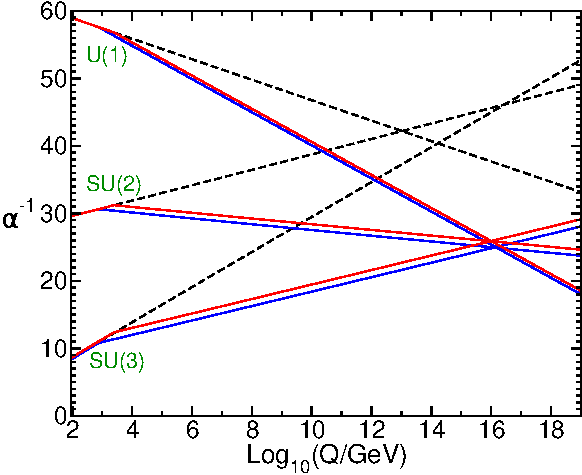
\includegraphics[width=\pairwidth]{figures/general/couplings}
 \caption{Running couplings for all three fundamental forces in case of the SM (dashed lines) and the minimal supersymmetric standard model (solid lines) for two different sparticle mass scales ($750\GeV$ and $2.5\TeV$)~\cite{SUSYPrimer}.}
 \label{fig:couplings}
\end{figure}



\section{Supersymmetry}\label{sec:SUSY}
Supersymmetry (SUSY)~\cite{SUSYOriginal,SUSYPrimer} is one of the most popular BSM theories and was developed in the 1970s~\cite{SUSYTheorem,HAAG1975257}. It is well motivated with regard to the theory, because it is the only possible extension of space time symmetry. Since then, many different SUSY models have been developed, all based on the same principle: SUSY connects fermions with bosons and the other way around by introducing supersymmetric partners for SM particles. These superpartners differ only in spin by $\pm1/2$, and all other quantum numbers are equal. With the help of generators $Q$, bosonic and fermionic states can be transformed into each other:
\begin{equation}
 Q\,\ket{fermion}=\ket{boson},~~~~~~ Q\,\ket{boson}=\ket{fermion}.
\end{equation}
Advantages of SUSY are, \eg, that multiple models directly provide candidates for dark matter particles, it realizes the unification of forces, and solves the Hierarchy Problem without fine tuning of physical parameters to match the observation.\\
The simplest model of SUSY regarding the extension of the particle content is the minimal supersymmetric standard model (MSSM), where only exactly one $Q$ exists. Within the MSSM, for each left and right-handed fermion in the SM exactly one supersymmetric scalar bosons is introduced. To differentiate between SM and SUSY particles, the names of supersymmetric partners are those of the SM particles prepended with an "s-" in case of the fermions. Thus the partners are called sfermions, and, \eg, the partner of the electron is the selectron. The names of superpartners of bosons are constructed by appending the SM name with an "-ino", making them bosinos, so the gluon's superpartner for example is called gluino. In general, superpartners are called sparticles, and are labeled the same as their SM counterparts, but with a tilde (\eg $\mu \to \widetilde{\mu}$). Also, the couplings between all sparticles are the same as of their SM partners.\\
To realize mass terms in the spontaneous symmetry breaking for all particles, including both up- and down-type fermions, the SM Higgs sector needs to be extended to two complex scalar doublets:
\begin{equation}
 H_u=  \left(
 \begin{matrix}
  H_u^+ \\
  H_u^0
 \end{matrix}
 \right),~~~~~
 H_d=  \left(
 \begin{matrix}
  H_d^0 \\
  H_d^-
 \end{matrix}
 \right).
\end{equation}
The $H_d$ gives masses to the down-type quarks and charged leptons, while the $H_u$ is responsible for the masses of up-type quarks. Four higgsinos as superpartners are introduced in the MSSM accordingly. As a consequence, there are eight degrees of freedom in the Higgs sector instead of four, related to the two Doublets, and giving rise to an expanded Higgs sector consisting of five particles: the two neutral scalars $h^0$ and $H^0$, the two charged scalars $H^{\pm}$, and the neutral pseudoscalar $A^0$. The remaining three degrees of freedom give masses to the gauge bosons as in the SM. The observed Higgs boson at the LHC can be identified as one of the two neutral scalars, where the lightest boson, the $h^0$, is chosen by convention.\\
The gauginos and higgsinos mix, similar to the mixing in the electroweak sector, to eight mass eigenstates, which are the four neutral neutralinos $\neutralinoOne,~\neutralinoTwo,~\neutralinoThree$,~and $\neutralinoFour$, and the four charged charginos $\charginoOne$ and $\charginoTwo$.\\
The total particle content of the MSSM is shown in \refFig{fig:mssm}. To include gravity, the SM is extended by the graviton $G$, and the SUSY sector is extended by its superpartner, the gravitino $\gravitino$.

\begin{figure}[tbp]
 \centering
 \includegraphics[width=0.8\textwidth]{figures/general/MSSM}
 \caption{The particle content of the MSSM extended with the graviton and gravitino. Mixings to mass eigenstates are indicates with the brackets.}
 \label{fig:mssm}
\end{figure}

In unbroken SUSY, the particles and their corresponding sparticles should have the same masses, and those SUSY particles should have been found easily in the past (considering, \eg, a selectron with a mass of $511\keV$). Therefore, SUSY must be a broken symmetry. Many different theories have been developed over time to explain different breaking scenarios. Attractive approaches are models where gravity is responsible for the SUSY breaking~\cite{SUSYPrimer}, anomaly breaking scenarios~\cite{AMSB}, and in particular gauge-mediated supersymmetry breaking, which are discussed in the next section.\\
SUSY can provide Dark Matter candidates, if the lightest supersymmetric particle (LSP) is stable, electrically neutral, and colorless.
R-parity
\begin{equation}
 R = (-1)^{3B+L+S}
\end{equation}
is therefore introduced as a new conserved quantum number, where S is the spin, $B$ the Baryon number, and $L$ the lepton number. The R-parity is $-1$ for sparticles, and $+1$ for particles, respectively.\\
It is not fundamentally necessary that the LSP is stable. In R-parity violating scenarios, decays of all SUSY particles into SM particles are allowed. Hence, the conservation of the Baryon number or the lepton number is violated. R-parity conserving scenarios however are motivated by many precision measurements, such as the life time measurement of protons~\cite{ProtonDecay}.
In this thesis, only R-parity conserving scenarios are considered. Therefore, SUSY particles can only be produced in pairs and the LSP needs to be stable.\\



\subsection{General Gauge Mediation}\label{sec:GGM}
The phenomenology of SUSY is very rich. While in many models gravity is responsible for SUSY breaking, a different approach, motivating this search, is general gauge mediation (GGM). It is based on the assumption of gauge mediated supersymmetry breaking (GMSB)~\cite{GGM}, where an additional "hidden sector" is introduced that is responsible for the breaking. This sector is mainly decoupled, and the possible interactions between the visible and the hidden sector are only achieved by messenger fields mediated by gauge interactions. In the studied GMSB models, the LSP is the gravitino $\gravitino$. This particle is assumed to be very light ($\ll1\GeV$). Therefore, the next-to-lightest supersymmetric particle (NLSP), which basically can be any sparticle, decays promptly. Since the gravitino is stable because of R-parity conservation, electrically and color neutral, it will leave the detector undetected, causing an imbalance in the measured total transverse momentum in proton-proton collisions at the LHC.\\
In all models considered throughout this thesis, the NLSP is assumed to be the lightest neutralino ($\neutralinoOne$). In general, the mixing of the NLSP can include bino, wino, and higgsino components, each enabling different decay channels.


\subsection{Signal scenarios}\label{sec:SMS}
The signal scenarios considered in this thesis are discussed in the following. In general, very different production channels for SUSY particles, such as electroweak and strong production, are possible. In case of the LHC proton-proton collisions, SUSY particles can be produced directly in the hard scattering processes of the partons, leading to cascade decays down to the decays of the NLSP to the gravitino and a SM boson. The branching fractions of the lightest neutralino to different SM bosons depends on its mixing
\begin{equation}
 \neutralinoOne = \sum_{i=1}^{N} N_{1i} \widetilde{\psi}_i^0,
\end{equation}
where $\widetilde{\psi}_i^0=(\widetilde{B},\widetilde{W},\widetilde{H}_d^0,\widetilde{H}_u^0)$~\cite{NLSPDecay}. The mass eigenvectors $N_{1i}$ are defined by four parameters, namely the bino mass $M_1$ and the wino mass $M_2$ at the messenger scale, the supersymmetric Higgs mass term $\mu$, and $\tan{\beta}$, the ratio of the up-type to down-type Higgs vacuum expectation values. In GGM, a neutralino NLSP has three possible decay branches, all involving the $\gravitino$~\cite{NLSPDecay}:
% \begin{equation}
\begin{align}
 \Gamma\left(\neutralinoOne\to\gravitino+\PGg\right) & = |N_{11}c_W+N_{12}s_W|^2 \mathcal{A}                                                                                                                       \\
 \Gamma\left(\neutralinoOne\to\gravitino+\PZ\right)  & = \left(|N_{12}c_W - N_{11}s_W|^2 +\frac{1}{2}|N_{13}c_{\beta}-N_{14}s_{\beta}|^2\right)\left(1-\frac{m_{\PZ}^2}{m_{\neutralinoOne}^2}\right)^4 \mathcal{A} \\
 \Gamma\left(\neutralinoOne\to\gravitino+h\right)    & = \frac{1}{2}|N_{13}c_{\beta}+N_{14}s_{\beta}|^2\left(1-\frac{m_{h}^{2}}{m_{\neutralinoOne}^2}\right)^4 \mathcal{A}                                         
\end{align}
% \end{equation}
Here, $c_W$, $s_W$, $c_\beta$, and $s_\beta$ are abbreviations for $\cos(\theta_{\text{W}})$, $\sin(\theta_{\text{W}})$, $\cos(\beta)$, and $\sin(\beta)$, respectively. The formulae hold in cases of on-shell $\PZ$ and $h$ production. $\mathcal{A}$ is a parameter responsible for the NLSP lifetime~\cite{NLSP1,NLSP2}:
\begin{equation}
 \mathcal{A} = \frac{m_{\neutralinoOne}^5}{16\pi F_{0}^{2}}\approx\left(\frac{m_{\neutralinoOne}}{100\GeV}\right)^5\left(\frac{100\TeV}{\sqrt{F_0}}\right)^4 \frac{1}{0.1\mm},
\end{equation}
where $F_0$ is the scale of SUSY breaking, its range is given by $10\TeV\lesssim\sqrt{F_0}\lesssim10^6\TeV$, and it is related to the gravitino mass via
\begin{equation}
 m_{\gravitino}=\frac{F_0}{\sqrt{3}M_{Planck}}.
\end{equation}
% Branching fractions for pure bino- or wino-, or higgsino-like NLSPs are shown in \refFig{fig:BRNLSP}.
Branching fractions for pure bino- or wino-like NLSPs are shown in \refFig{fig:BRNLSP}.
\begin{figure}[htb]
 \centering
 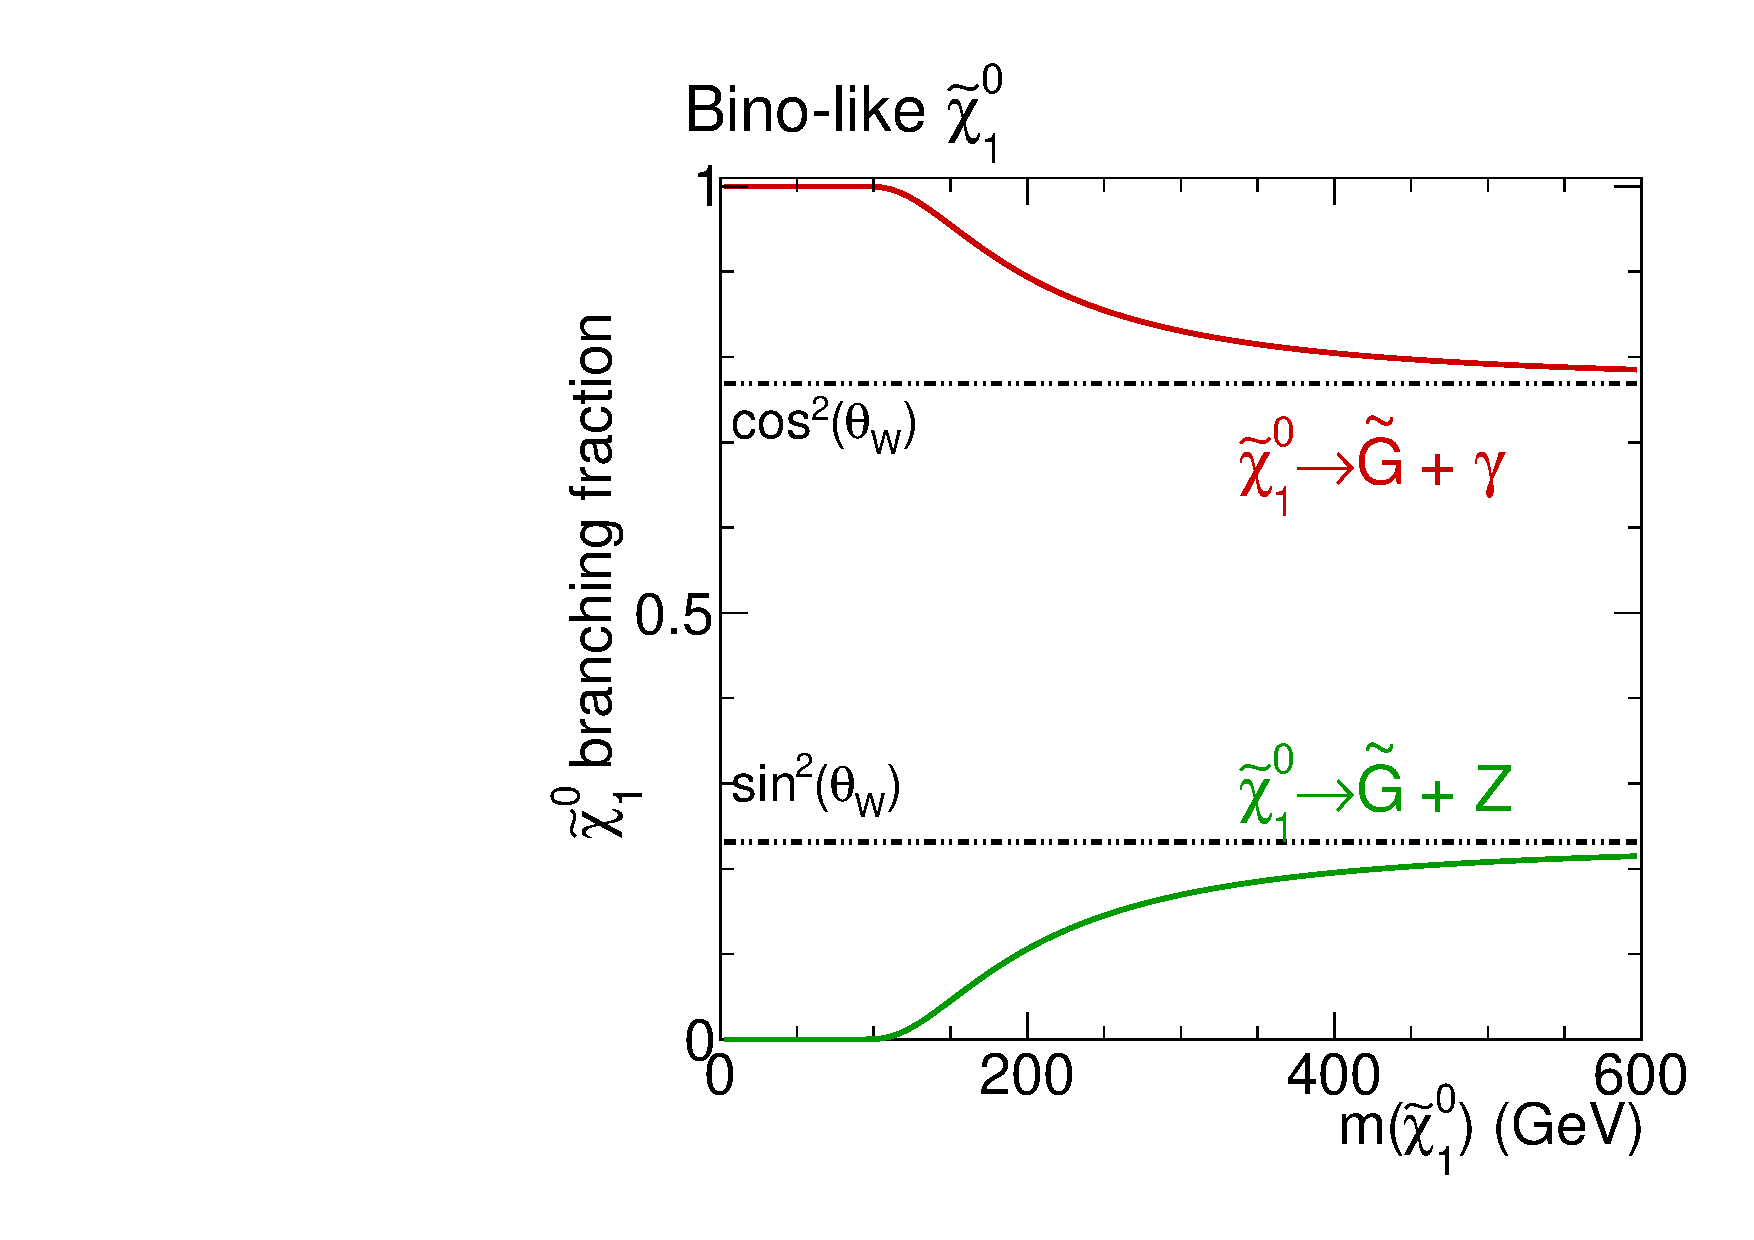
\includegraphics[width=\pairwidth]{figures/signal/binoBranching}
 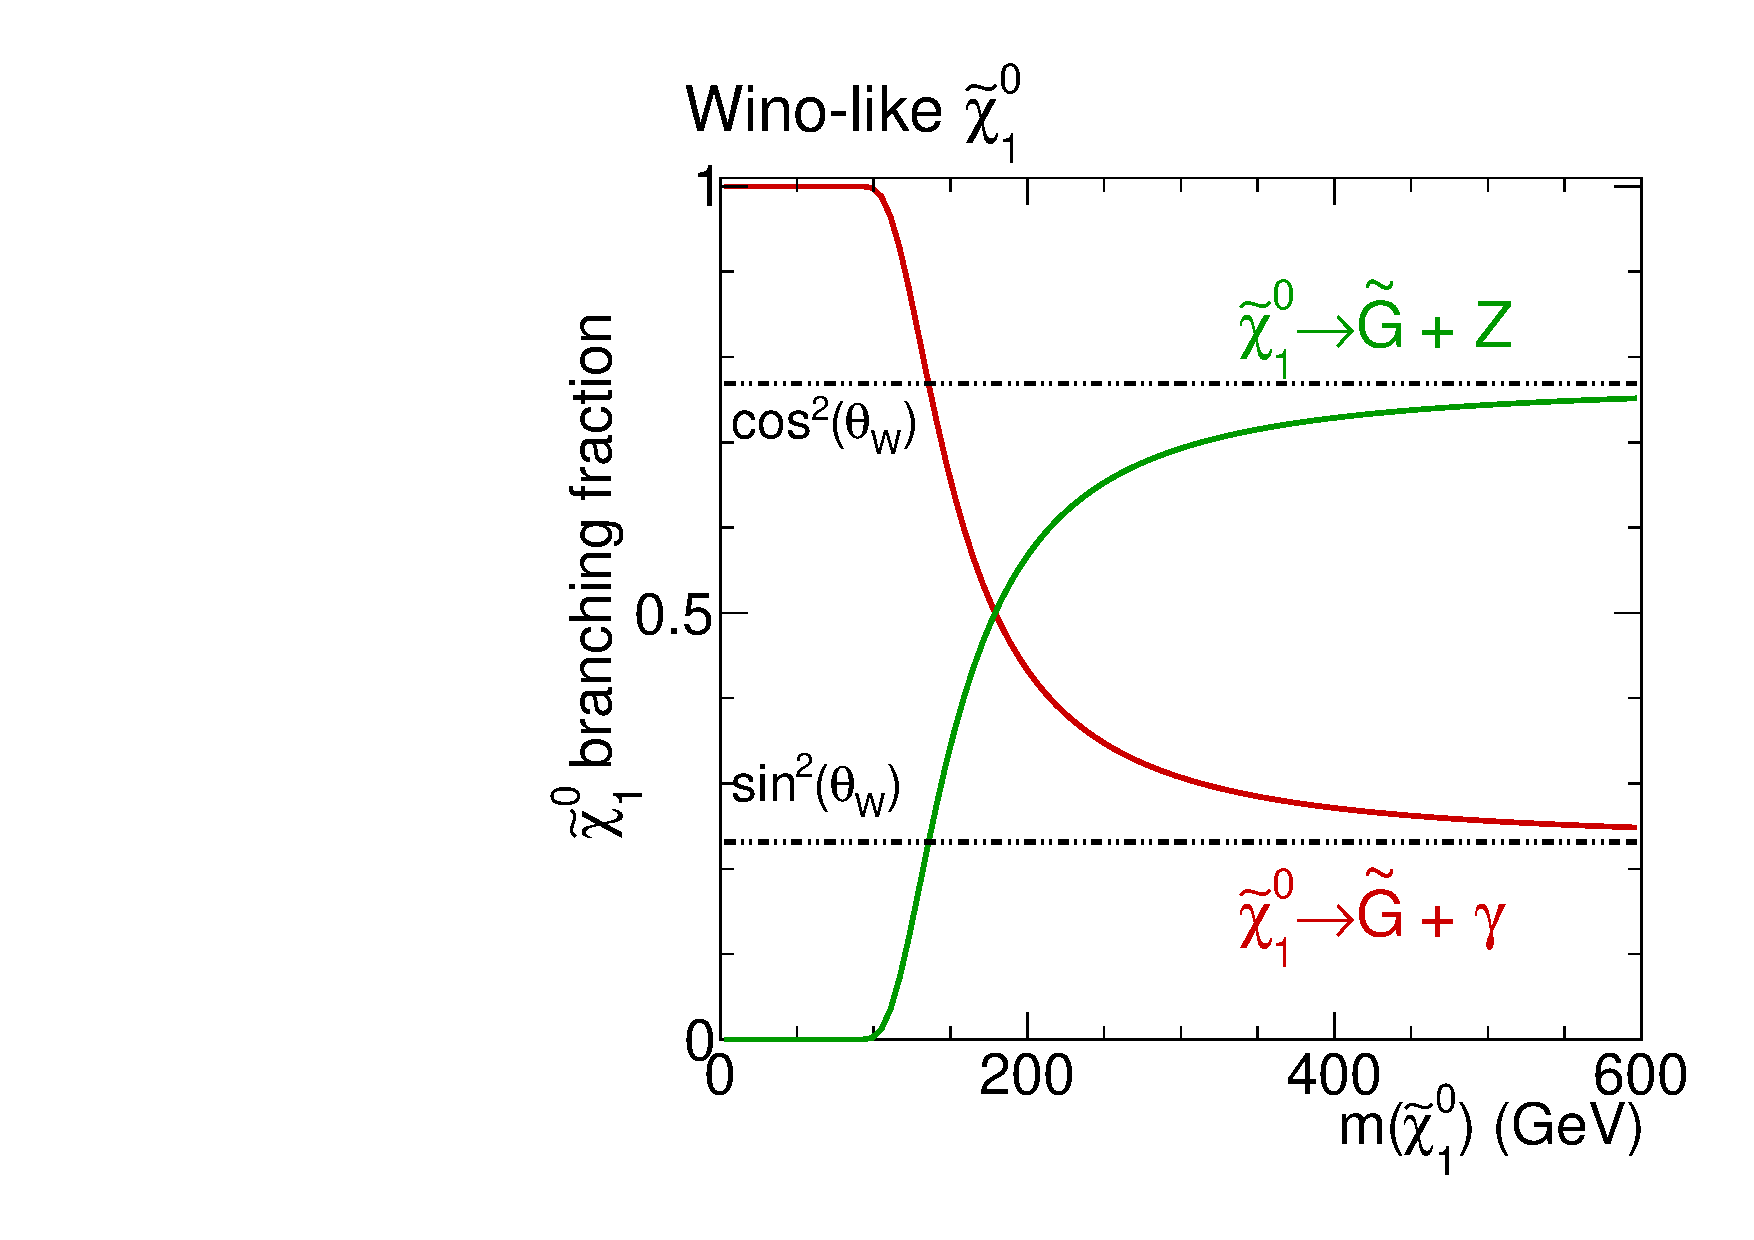
\includegraphics[width=\pairwidth]{figures/signal/winoBranching}%\\
 % 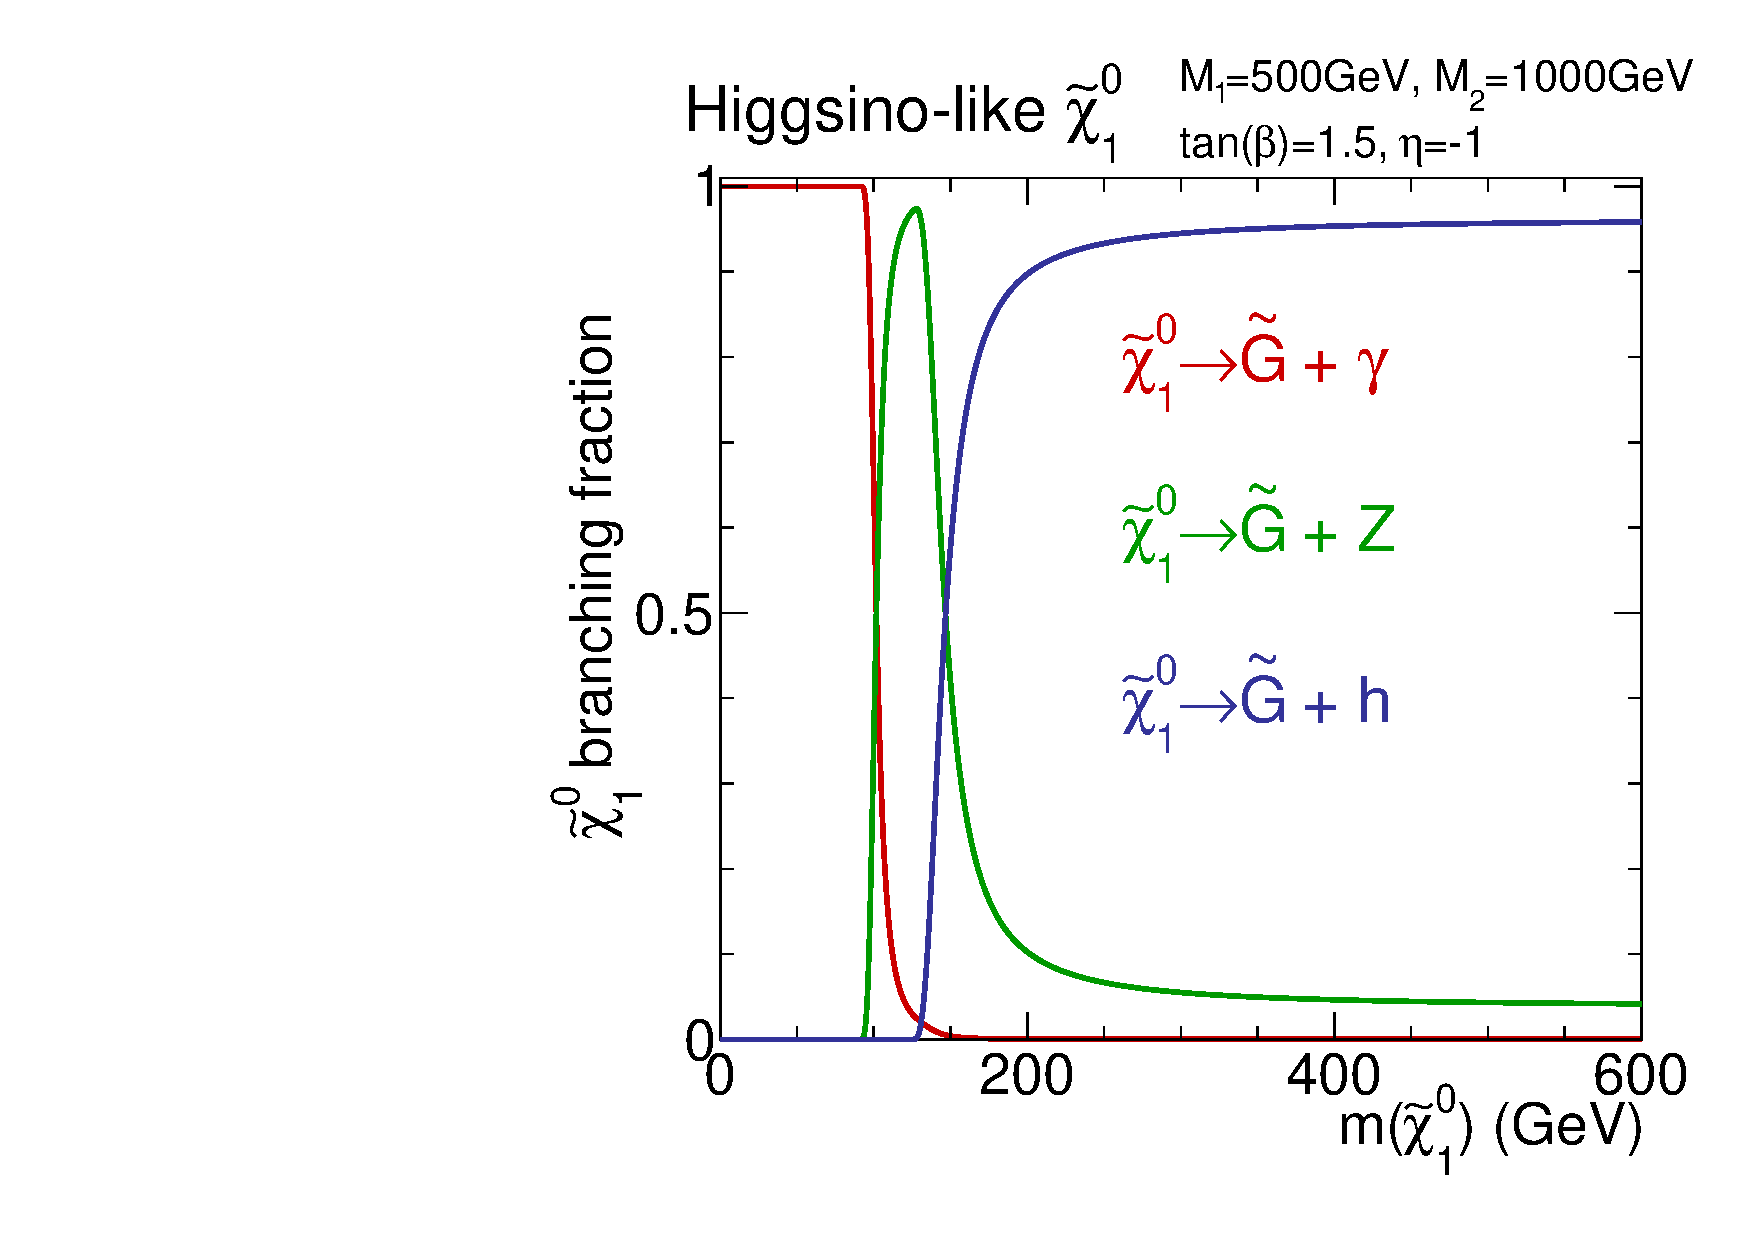
\includegraphics[width=\pairwidth]{figures/signal/higgsinoBranching1}
 % 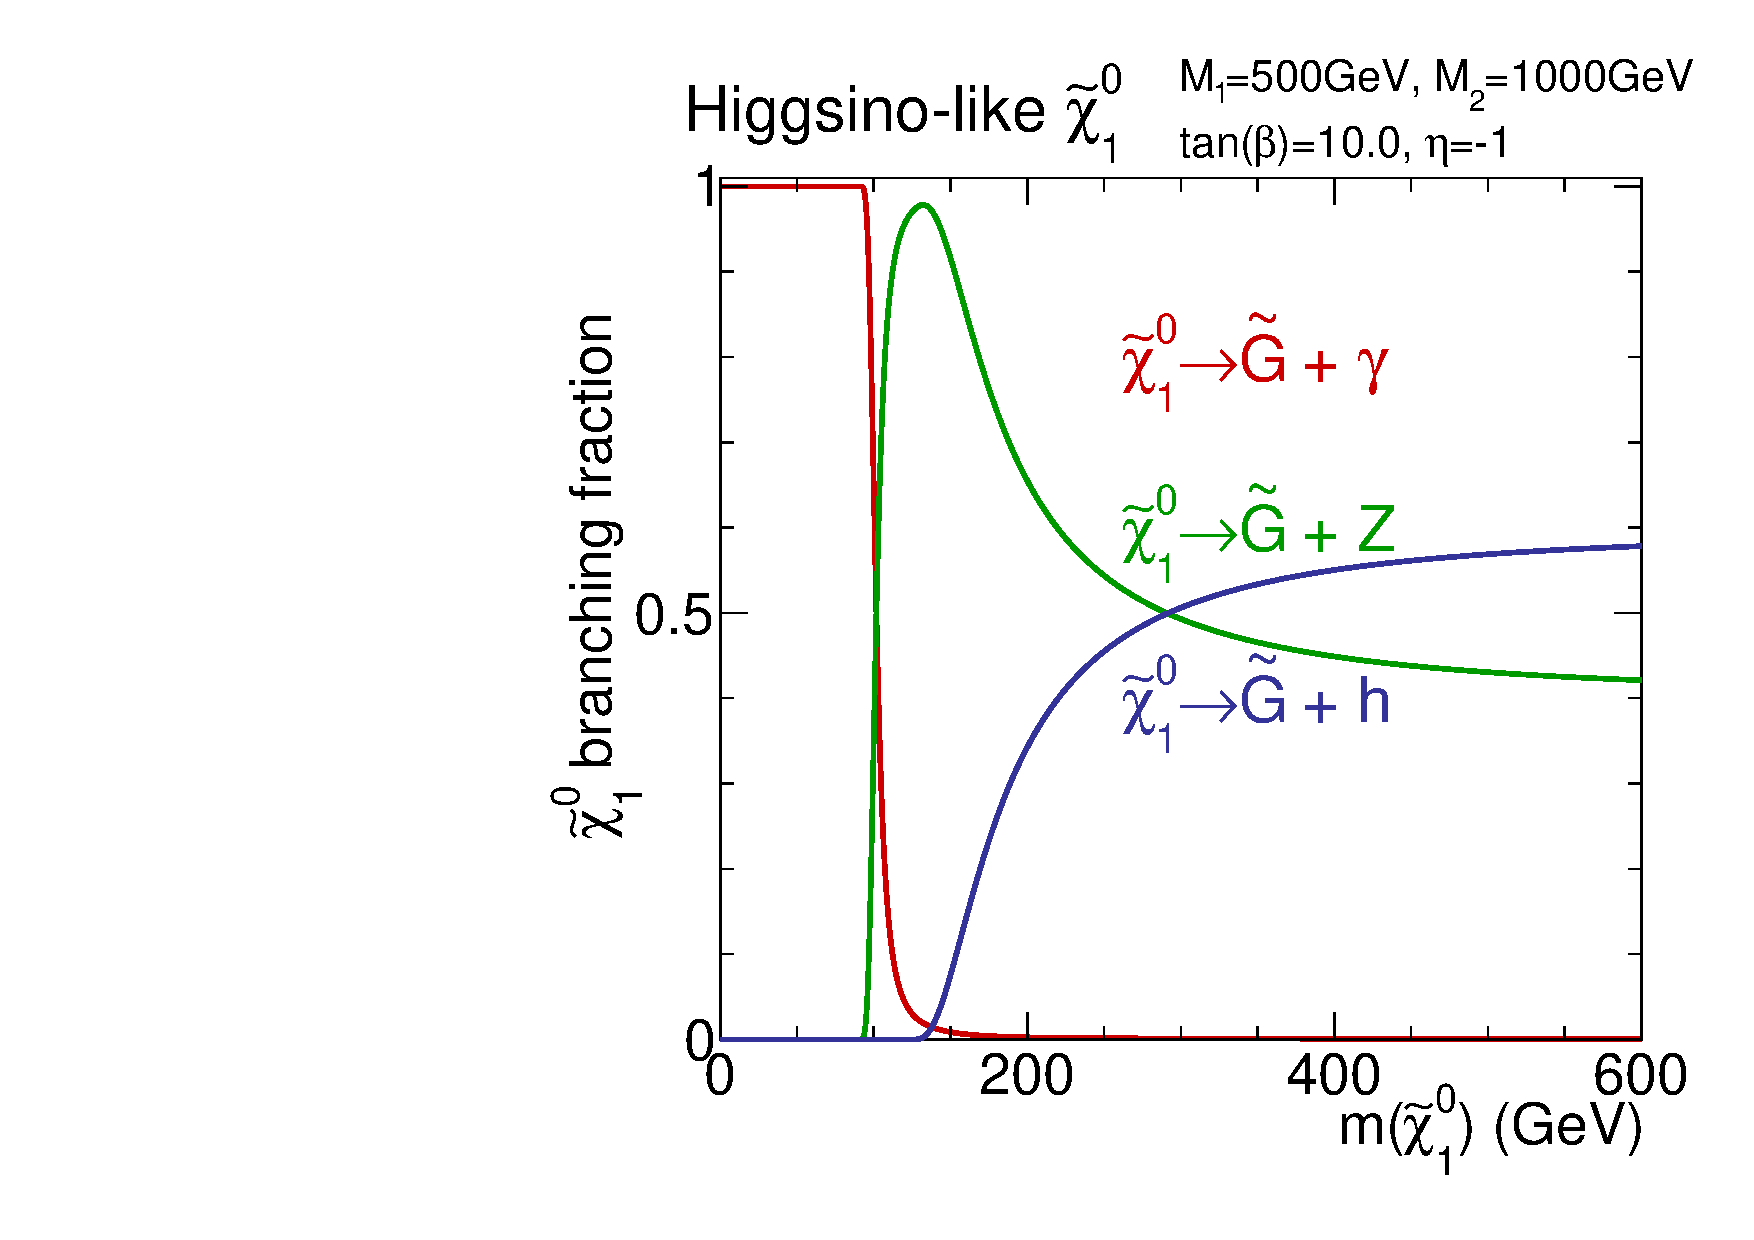
\includegraphics[width=\pairwidth]{figures/signal/higgsinoBranching2}
 % \caption{Branching fractions for pure bino (top left), wino (top right), and two higgsino-like (bottom) NLPS scenarios with different parameters. The parameter $\eta$ is defined as $\eta=sgn(\mu)$.}
 \caption{Branching fractions for pure bino (left) and wino (right) NLPS scenarios with different parameters.}
 \label{fig:BRNLSP}
\end{figure}
Since the final state investigated in this analysis consists of a $\PZ$ boson and a photon, the search is sensitive in particular to bino- and wino-like NLSP scenarios.\\\\
One scenario used in the development of this search is a consistent GGM model, where the NLSP is the $\neutralinoOne$, and it is assumed to be bino-like. The heavier neutralino $\neutralinoTwo$ and the lightest chargino $\charginoOne$ are assumed to be wino-like. Therefore, the bino mass equals the mass of the lightest neutralino, while the $\PSGcpDo$ and the $\PSGczDt$ are mass degenerate and their mass equals the wino mass. Higgsinos are decoupled, \ie, set to very high masses. Squarks and gluinos are also decoupled in this scenario, allowing only electroweak production modes. For the most dominant process a diagram is shown in \refFig{fig:ewkSMS} right. The signal cross section depends only on the wino mass, since $\neutralinoTwo\PSGcpmDo$ and $\PSGcmpDo\PSGcpmDo$ production are by far the most dominant production channels. The branching fractions of the gauginos are given by the gaugino masses and their gauge eigenstates, and behave as shown in \refFig{fig:BRNLSP}. The mass of the neutralinos and the lightest chargino directly influence the transverse momenta in the final state. As can be seen in \refFig{fig:ewkSMS}, larger mass differences between the NLSP mass and the wino mass will lead to higher momenta of the produced bosons in the cascades. The mass of the NLSP is directly responsible for the momenta of the SM bosons and the gravitino in the final state, and therefore the missing transverse momentum in an event.
\begin{figure}[tbp]
 \centering
 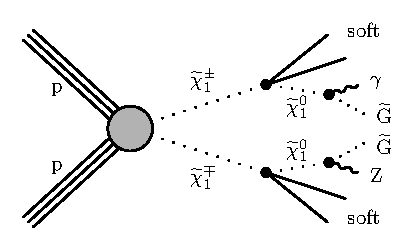
\includegraphics[width=0.49\textwidth]{figures/signal/TChiNG}
 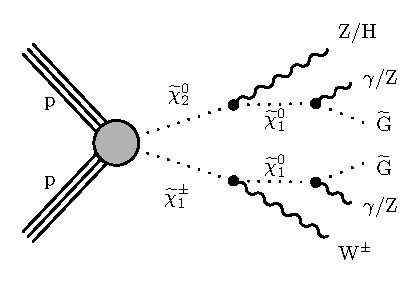
\includegraphics[width=0.49\textwidth]{figures/signal/gmsb}
 \caption{Diagram of the \texttt{TChiZG} scenario (left) with chargino pair production, where the charginos decay to neutralinos under soft emission of off-shell W bosons. Also, the chargino-neutralino production is possible. The most dominant production process with a wino-like $\PSGcpDo$ and $\PSGczDt$ of the full GMSB model (right).}
 \label{fig:ewkSMS}
\end{figure}
\\\\A very different approach in regard to the interpretation in full theoretical models are simplified models (SMS)\cite{SMS}. Here, only a limited particle content is assumed with simplified assumptions on the production and decay channels, providing a more model independent result by probing distinct final states. These results can be reinterpreted in various models~\cite{SMSReInt}. In this thesis two simplified models are considered, one with electroweak gaugino production, and the other one with a strong gaugino production channel.\\
The electroweak model is the \texttt{TChiZG} SMS, in which only neutralino-chargino and chargino-chargino production is assumed. The lightest chargino and lightest neutralino are assumed to have nearly the same mass, leading to soft emissions of off-shell W bosons in the decays of the charginos to the NLSP. The branching fractions of the lightest neutralino to a gravitino and a photon or a Z boson are fixed to $50\%$ each, \ie, $\mathcal{BR}(\PSGczDo\to\gamma\gravitino)=\mathcal{BR}(\PSGczDo\to\PZ\gravitino)=0.5$. A diagram for the process can be found in~\refFig{fig:ewkSMS} left. The squarks and gluinos are decoupled.\\
The strong model considered here is the \texttt{T5bbbbZG} SMS. A diagram is depicted in \refFig{fig:strongSMS}. In this model, gluino pair production is assumed, leading to decays to the NLSP under the emission of bottom quark pairs. The branching fractions for the $\PSGczDo$ to photons and Z bosons are again set to $50\%$ each.

\begin{figure}[tbp]
 \centering
 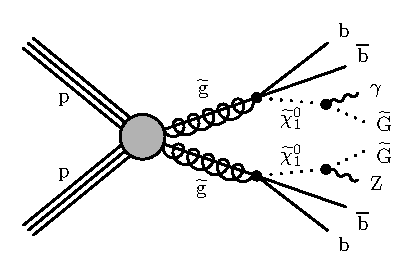
\includegraphics[width=0.49\textwidth]{figures/signal/T5bbbbZG-crop}
 \caption{The Feynman diagram for the \texttt{T5bbbbZG} scenario with pair production of gluinos in the hard process, decaying to neutralinos under the emission of b quarks.}
 \label{fig:strongSMS}
\end{figure}


\subsection{Status of SUSY searches at the Large Hadron Collider}
Searches for SUSY have been performed  at the LEP experiment~\cite{LEP}, the Tevatron collider~\cite{TEVATRON}, and using the LHC Run~I data~\cite{ChristianRunI}. Although some promising excesses with respect to the SM expectation have been observed for example in the opposite-sign dilepton channel~\cite{Edge}, no clear evidences for SUSY or other BSM theories have been confirmed. Currently SUSY is also constrained by precision measurements of the Higgs boson properties as mentioned above, and by measurements of rare decay processes, such as the $B_S^0\to\Pgmm\Pgmp$ decay observed by the CMS and LHCb collaborations~\cite{B0S}. In the SM, this decay is helicity suppressed, whereas in the MSSM or other extensions to the SM this decay may receive large enhancements.\\
Direct searches for SUSY in terms of SMS interpretations excluded gluino pair production up to gluino masses of around $2\TeV$~\cite{GluinoCMS}, squark pair production up to squark masses of roughly $1500\GeV$, and sbottom (stop) masses of approximately $1500\GeV$~\cite{sbottom} ($1200\GeV$~\cite{stop}), respectively. The production of electroweakinos (electroweak gauge bosinos) is excluded for chargino and neutralino masses up to around $1.1\TeV$~\cite{EWKinos}.
Regarding GMSB scenarios, the currently most stringent exclusion limits set by the CMS collaboration~\cite{CMS} are shown in \refFig{fig:GMSB_summary}.
\begin{figure}[tbp]
 \centering
 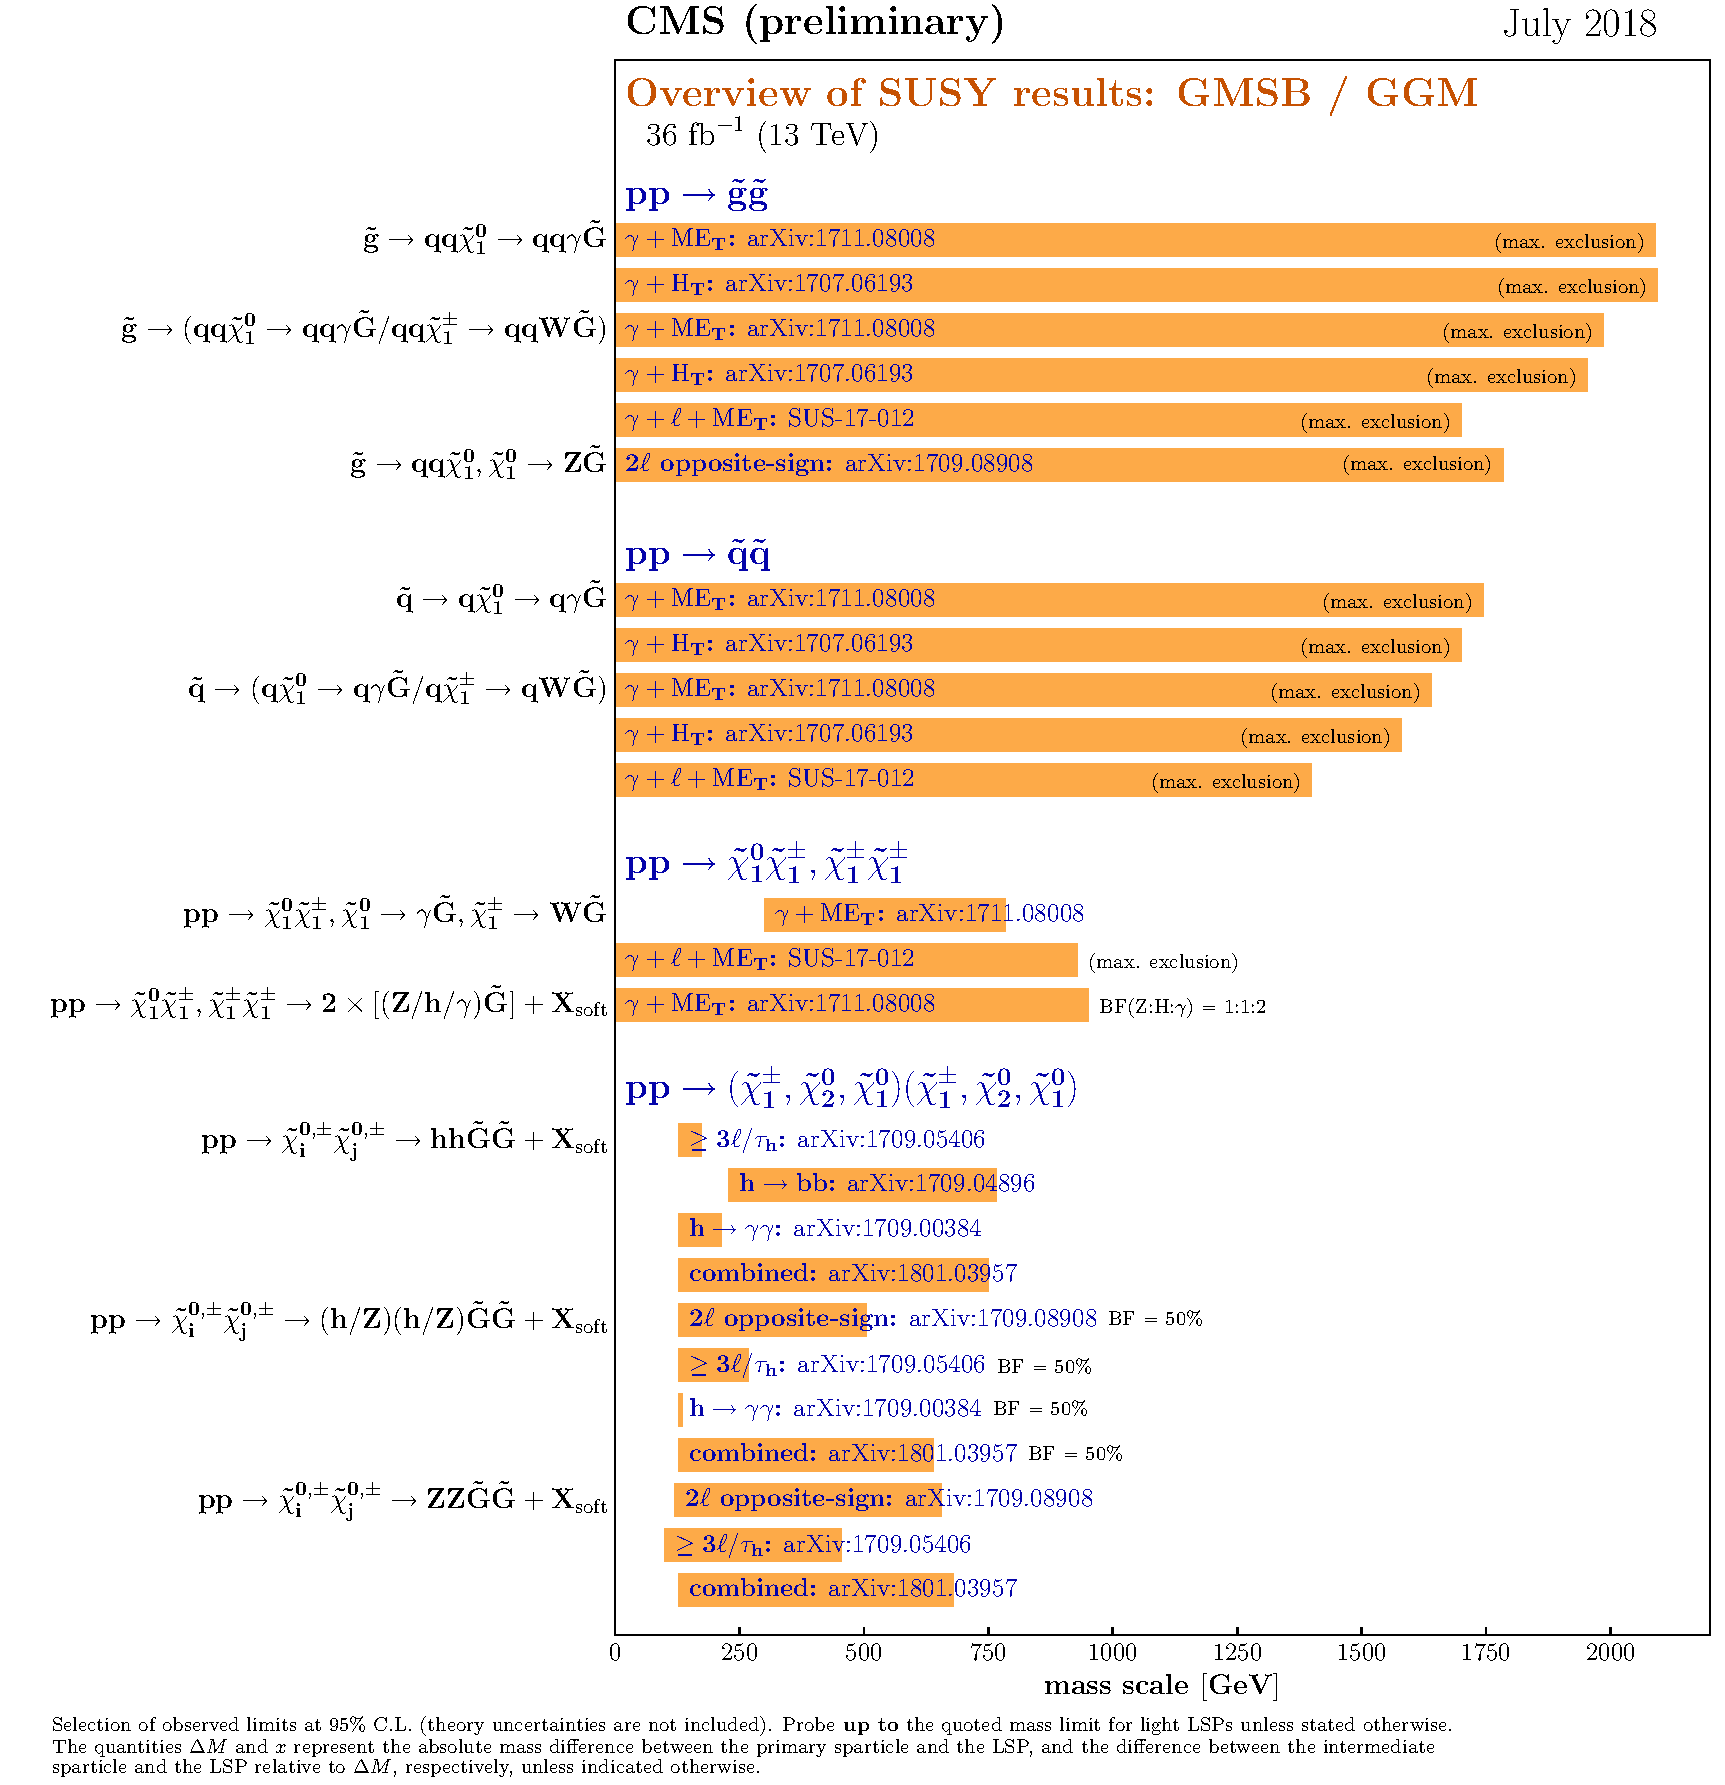
\includegraphics[width=0.99\textwidth]{figures/general/barplot_GMSB}
 \caption{Mass exclusion limits for simplified models in the context of GMSB~\cite{SUSSummaryPlot} of the CMS collaboration.}
 \label{fig:GMSB_summary}
\end{figure}
The presented results are based on the proton-proton collision data recorded with the CMS detector in 2016, corresponding to an integrated luminosity of $36\fbinv$ with a center-of-mass energy of $\sqrt{s}=13\TeV$. Searches similar to the one presented in this thesis exclude electroweakino production scenarios up to roughly $980\GeV$, when final states tagged with a high-energy photon and large missing transverse momentum are analyzed~\cite{PhotonMet}. Searches targeting the single lepton plus photon final state~\cite{PhotonLepton} have set lower limits. Strong exclusions for gluino and squark pair production scenarios are set by searches targeting events with large hadronic activity and photons~\cite{PhotonHT} and searches investigating events with photons together with high b-jet multiplicity~\cite{PhotonBJet} over the whole parameter space. They set limits up to approximately $2.2\TeV$ for gluino masses and $1.8\TeV$ for squark masses.\\
Despite the high exclusion limits set by CMS and ATLAS analyses~\cite{AtlasGMSB1,AtlasGMSB2,AtlasGMSB3} in comparable ways, large regions of phase space remain unexplored. But since there are many different SUSY models, and the phenomenology of SUSY is very rich, including scenarios with R-parity violation, compressed mass spectra, long-lived particles and displaced vertices, all described in different breaking scenarios, many studies and searches are yet to be performed. Nevertheless, although the sparticle masses are not predicted by theory, natural SUSY scenarios without great fine tuning should lead to sparticle masses in the order of $\mathcal{O}(\TeV)$, which are accessible at the LHC~\cite{SUSYNaturalStatus}.

\chapter{The Experiment}\label{chap:experiment}
In this chapter, the relevant experimental setup is explained. Starting with the description of the Large Hadron Collider (LHC), which is responsible for the acceleration of the proton beams, after that the Compact Muon Solenoid (CMS) experiment and detector with all important subdetector components is explained.
\section{The large hadron collider}\label{sec:LHC}
The Large Hadron Collider~\cite{LHC1,LHC2}, located at the European Organization of Nuclear Research (CERN) near Geneva in Switzerland, is the worlds largest hadron collider. The design center-of-mass energy for the proton-proton collisions is $\sqrt{s}=14\TeV$, while the LHC started operating in 2010 with an energy of $7\TeV$. After running also in 2011 at $7\TeV$, the energy was increased for the 2012 run period to $8\TeV$. After the end of RunI, and after the first long shutdown, the LHC started running again in 2015 with an increased center-of-mass energy of $13\TeV$. This setup was maintained trough the whole RunII until the end of 2018. In the following, the LHC will be upgraded again in the long shutdown II, so that with the beginning of 2021 it is planned to start operating with the design energy of $14\TeV$.
In addition, the LHC is capable of accelerating lead ions with an energy of $2.76\TeV$ per nucleon.\\
The LHC is a synchroton collider built in a tunnel with a circumference of $27\km$, which was already used for the Large Electron Positron collider (LEP)~\cite{LEPCollider} in the past. The proton beams are accelerated using various preacceleators, such as the Booster, Proton Synchroton (PS), and the Super Proton Synchroton (SPS), delivering an proton energy of $450\GeV$ before entering the main storage ring. Four main experiments are located at the LHC, each built around one of the four collisions points. These namely are: CMS (Compact Muon Solenoid)~\cite{CMS}, ATLAS (A Toroidal LHC Apparatus)~\cite{ATLAS}, ALICE (A Large Ion Collider Experiment)~\cite{ALICE}, and LHCb (LHC Beauty)~\cite{LHCb}. CMS and ATLAS were designed to be independent experiments looking both for BSM physics, measure precisely properties of the SM, and improve the knowledge on the Higgs sector. Besides those tasks, they also analyze lead ion collisions to gain a deeper understanding of the strong interaction. The tasks of ALICE include studies on the quark-gluon-plasma, where the confinement is abrogated, leading to asymptotically free quarks and gluons. LHCb investigates mainly mesons that include charm and bottom quarks, to perform precision measurements of the SM and indirectly look for $\mathcal{CP}$-violation and hints for new physics. The asymmetric detector design of LHCb favors such studies, since the forward region with particles flying close to the beam axis, is enriched with that kind of events. A schematic sketch of the LHC apparatus including the four big experiment locations and interaction points, and the preaccelerators, is shown in \refFig{fig:LHC}.\\
\begin{figure}[hbtp]
 \centering
 \includegraphics[width=0.89\textwidth]{figures/general/LHC}
 \caption{A sketch of the total LHC accelerator complex~\cite{LHCPicture}. The four main experiments are marked as yellow dots, and the preacceleators are also shown.}
 \label{fig:LHC}
\end{figure}
As the protons are accelerated to an energy of $450\GeV$, they are injected as bunches of approximately $N=1.1\cdot10^{10}$ particles into the two beam pipes counter rotating in intervals of $25\ns$. To achieve a center-of-mass energy of $13\TeV$, each beam has to reach an energy of $6.5\TeV$. Therefore, superconducting cavities operating at $400\MHz$ accelerate the protons, and dipole magnets force the beams on their orbital path. Higher order multipoles are needed to focus the beam and correct for different beam and magnetic effects.\\
One important quantity to characterize a collider is the instantaneous luminosity $L$, because the rate of a distinct scattering process is proportional to $L$. It can be defined as
\begin{equation}
 L = \frac{N_{b}^2 n_{b} f_{rev} \gamma} {4\pi \epsilon \beta^{*}}F,
\end{equation}
where $N_b$ is the number of particles per bunch, $n_b$ the number of bunches, $f_{rev}$ the revolution frequency, $\gamma$ the relativistic Lorentz factor, $\epsilon$ the normalized transverse emmitance of the beam, $\beta^{*}$ the beta function at the interaction point, and $F$ a geometrical factor accounting for the cross section angles of the beams. The integrated Luminosity $\Lumi$ is related to $L$ via
\begin{equation}
 \Lumi= \int L dt.
\end{equation}
And the number of events $N$ for a given process with cross section $\sigma$ is given by
\begin{equation}
 N= \Lumi \cdot \sigma.
\end{equation}

In 2016 the LHC provided a total integrated luminosity of $40.82\pbinv$, while the CMS detector recorded $37.76\pbinv$, and $35.92\pbinv$ were validated to be used for physics analysis~\cite{DataQuality}.





\section{The compact muon solenoid detector}\label{sec:CMS}
The data used in this thesis was recorded by the CMS detector~\cite{CMS,CMSTDR} in 2016. The CMS detector is a multi-purpose detector housing different subdetector components. From inside to outside these are the tracker system including a pixel and the silicon strip detector, the electromagnetic calorimeter, the hadronic calorimeter, followed by the solenoid and the muon system. A cross section picture of the, CMS detector is shown in~\refFig{fig:CMS}. In the following, each subdetector and the trigger system will be briefly explained.\\
\begin{figure}[hbtp]
 \centering
 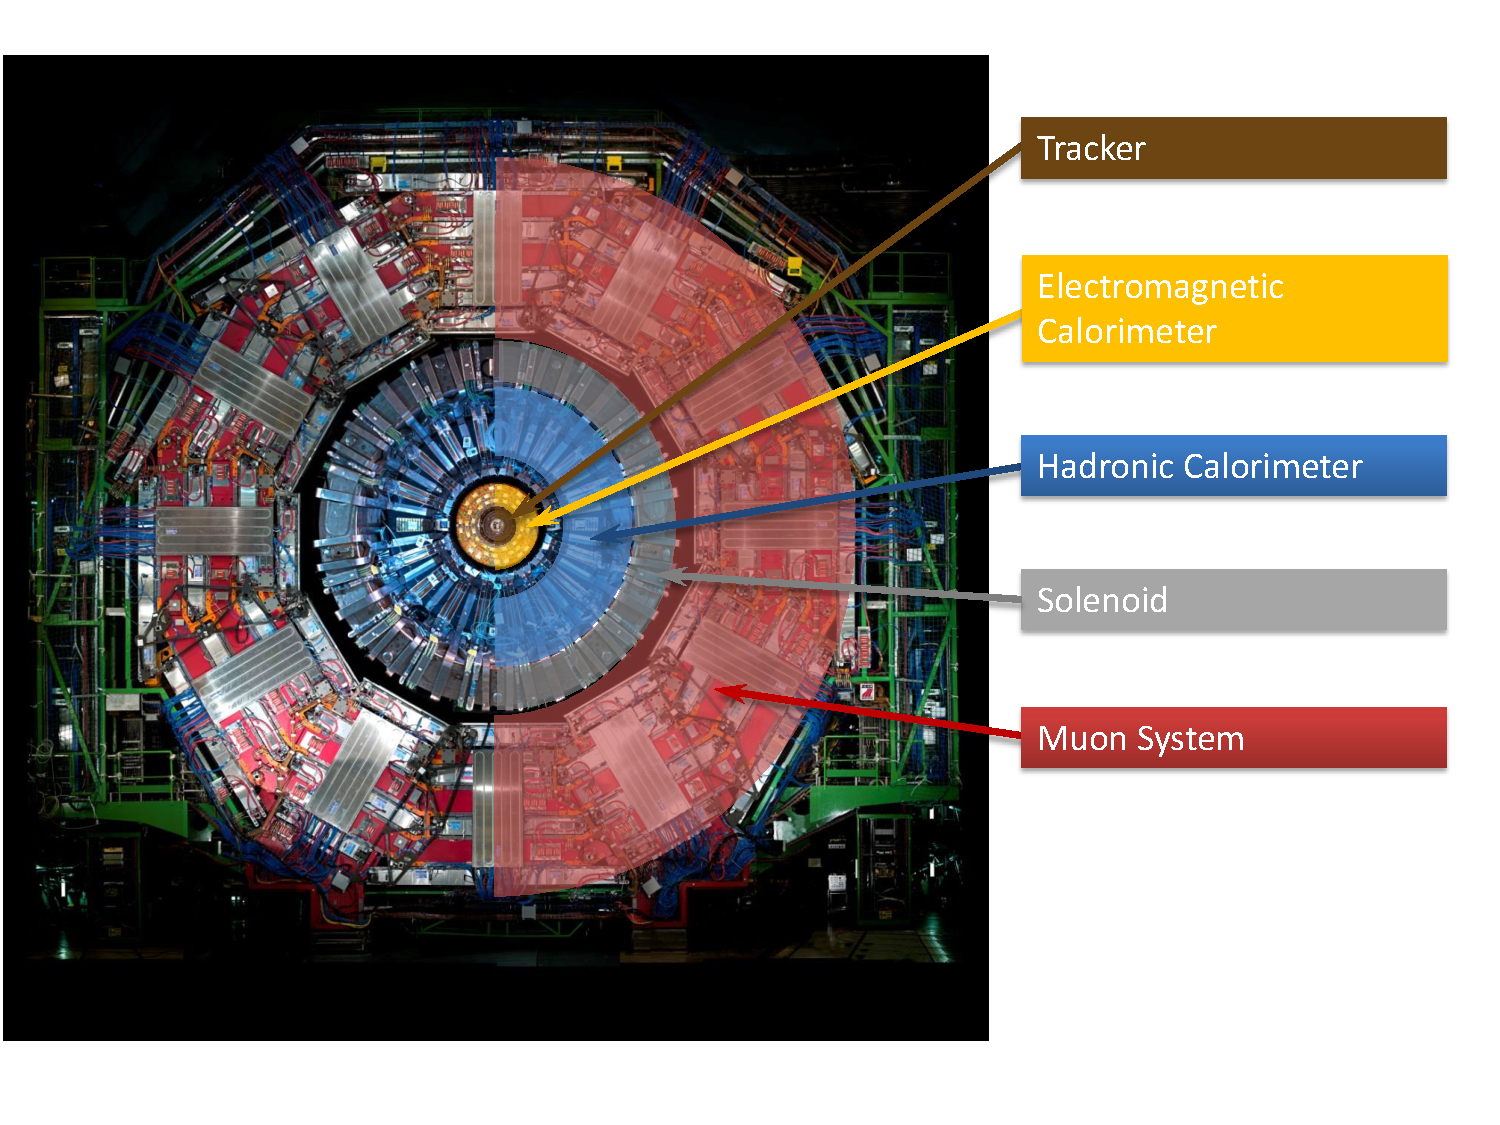
\includegraphics[width=0.99\textwidth]{figures/general/CMS}
 % 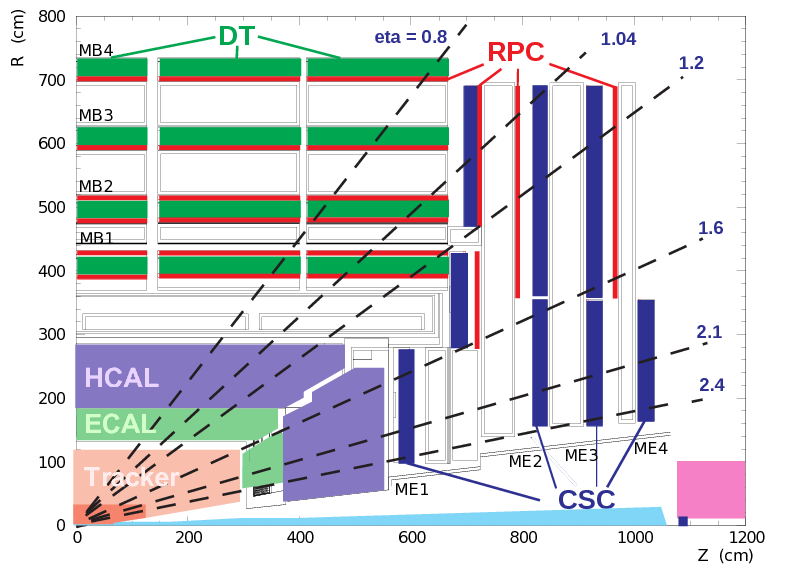
\includegraphics[width=0.49\textwidth]{figures/general/CMS_eta.png}
 \caption{A cross section picture of the open CMS detector~\cite{CMSPicture}. The important parts are labeled.\todo{Fixen oder Bild ersetzen!}}
 \label{fig:CMS}
\end{figure}
The coordinate system used to describe the detector is originated at the interaction point, and the z-axis points in the direction of the beam axis. The y-axis points upwards, while the x-axis points to the center of the LHC ring. To exploit the underlying symmetry of the detector, a transformation to an angular coordinate system is chosen. The azimuthal angle $\phi$ is measured in the x-y plane, while $\phi=0$ equals the direction of the x-axis, and $\phi$ ranges from $-\pi$ to $\pi$. The polar angle $\theta$ is measured from the positive z-axis, and the pseudorapidity $\eta$ can be introduced
\begin{equation}
 \eta=-\ln\left(\tan\left(\frac{\theta}{2}\right)\right).
\end{equation}
The advantage in using $\eta$ instead of $\theta$ is, that differences in $\theta$ are invariant under Lorentz-boosts along the beam axis.\\
In proton proton collisions, the initial total momentum of the colliding partons is unknown, since they carry only a fraction of the proton energy. But the transverse momentum in the initial state is negligible, and therefore, the transverse momentum
\begin{equation}
 \pt=|\ptvec|=|\vec{p}\cdot\sin(\theta)|
\end{equation}
is a widely used quantity.
Most of the subdetectors are divided in a low $\eta$ part (barrel), and two high $\eta$ parts (endcaps). Each of the subdetectors is designed to measure special properties of different particle types, to ensure both a good particle distinction and identification, and precise measurements of energy, momenta, and trajectories.



\subsection{Tracker system}
The most inner part of the CMS detector is the inner tracker, and it consists of two main components, a silicon pixel and a silicon strip detector\footnote{The silicon pixel detector was replaced at the end of the 2016 run. Since in this thesis only 2016 data is used, only the former detector is described.}. Both components enclose parts parallel to the beam pipe in the barrel, and parts orthogonal to the beam axis in the endcaps. They cover a length of $5.8\m$ and a diameter of $2.5\m$. A sketch of the total inner tracker is shown in \refFig{fig:tracker}. The tracker is designed to perform a precise measurement of particle trajectories and an identification of primary and secondary vertices. Therefore, a high granularity and fast response is needed. The silicon pixel subcomponent is built of three barrel layers (the closest at a radial distance of $4.4\cm$ to the beam pipe) and two endcap disks, covering a total area size of around $1\m^2$. Each of the $\approx66$ million silicon pixel cells has a size of $100\times150\micron^2$. This enables good resolution in all orientations independent of the track direction.\\
The silicon strip detector consists of four strip layers in the inner (TIB), and six layers in the outer part (TOB). In the direction of the endcaps, it is built of three inner disk layers (TID), and nine layers in the outer part (TEC).\\
The inner tracker in total covers a range of $|\eta|<2.5$ and has a size of around $200\m^2$. The performance of the tracker yields a momentum resolution for muons with a transverse momentum of $\approx100\GeV$ of $1-2\%$ in the pseudorapidity range of $|\eta|<1.6$. At higher pseudorapidities the momentum resolution decreases due to a lower granularity.

\begin{figure}[hbtp]
 \centering
 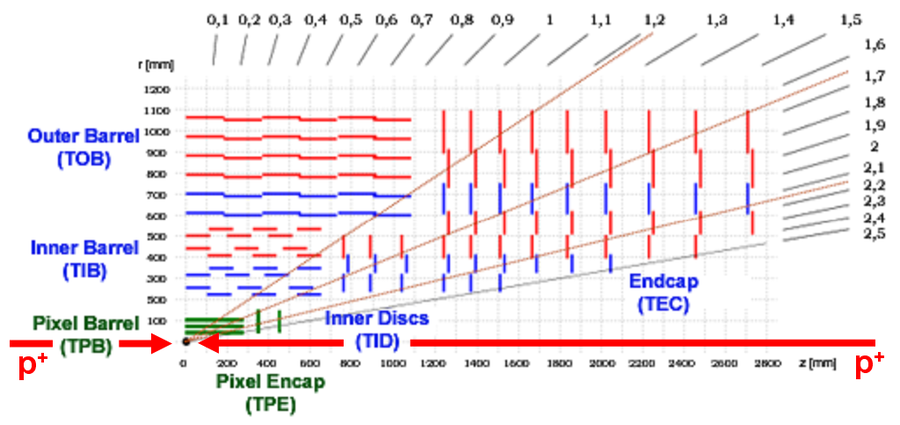
\includegraphics[width=0.69\textwidth]{figures/general/tracker.png}
 \caption{A sketch of one quadrant of the CMS inner tracker~\cite{TrackerPicture}.}
 \label{fig:tracker}
\end{figure}

\subsection{Electromagnetic calorimeter}
Around the tracker, the second subdetector of CMS is the electromagnetic calorimeter (ECAL). Its main purpose is to measure the energy of electrons and photons, which behave very similar in the detector. Together with the measurements of the tracker, a differentiation between electrons and photons can be performed. It is made homogeneously of lead-tungstate ($PbWO_4$) crystals, that emit light proportional to the deposited energy of trespassing particles in an electromagnetic shower. The emitted light, which is located in the visible spectrum, is measured by avalanche photomultipliers. The material of lead-tungstate was chosen due to its high density, short Moli\`{e}re radius of $2.2\cm$ characterizing the shower width, and short radiation length of $0.89\cm$. Another big advantage of $PbWO_4$ is she short scintillation time. In a time window of $25\ns$ most of the visible light ($\approx80\%$) is emitted, thus suiting very well the bunch spacing of $25\ns$. The crystals have a length of $23\cm$, matching $25.8$ radiation lengths. So in total both a compact format and a high granularity could be maintained.\\
The ECAL is divided into a barrel (EB: $|\eta|<1.479$) and an endcap part (EE: $1.479<|\eta|<3.0$), as can be seen in \refFig{fig:etaPlaneCMS}.
\begin{figure}[hbtp]
 \centering
 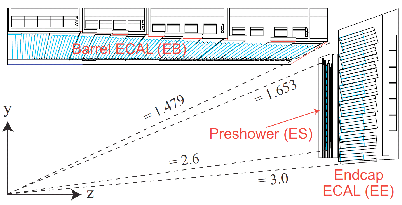
\includegraphics[width=0.49\textwidth]{figures/general/ecal}
 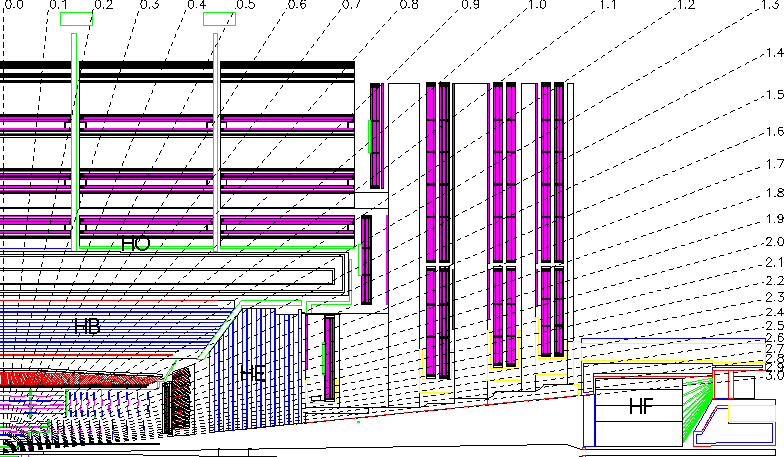
\includegraphics[width=0.49\textwidth]{figures/general/hcal}
 \caption{A sketch of one quadrant of the CMS detector for the ECAL (left)~\cite{ECALPicture}, and HCAL (right)~\cite{CMS}.}
 \label{fig:etaPlaneCMS}
\end{figure}
The total energy resolution of the ECAL is determined to be
\begin{equation}
 \left(\frac{\sigma_E}{E}\right)^2=\left(\frac{2.8\%}{\sqrt{E[\GeV]}}\right)^2 + \left(\frac{0.12}{E[GeV]}\right)^2 + (0.30\%)^2,
\end{equation}
where the first term covers stochastic effects due to the Poissonian distributed number of created scintillation photons, and the second term combines noise effects both from the electronics and multiple collisions per bunch-crossing (pile-up). The third term covers constant effects, such as intercalibration effects between the crystals and energy leakage~\cite{ECALRes}.\\
An additional preshower detector is installed in front of the ECAL endcap, to identify photons coming from meson decays.

\subsection{Hadronic calorimeter}
The hadronic calorimeter (HCAL), which is designed for the energy measurement of hadrons, consists also of a barrel (HB) and endcap parts (HE). It is placed between the ECAL at a radius of $1.77\m$ and the coil at a radius of $2.95\m$. An additional outer barrel part with lower granularity (HO) extends the HCAL outside of the solenoid, making use of its stopping power, while the hadron forward (HF) is installed to cover high pseudorapidity ranges. The barrel part covers pseudorapidities in the range of $|\eta|<1.4$, while the HCAL endcap together with the outer HCAL covers the range of $1.3<|\eta|<3$.\\
In contrast to the homogeneous ECAL, the HCAL barrel consists of alternating layers of brass and plastic scintillating material. The front and backplates are made of steel. Hence, the brass plates stop the incoming particles, and the energy deposit is measured in the form of hadronic showers creating scintillation light in the plastic layers. The outer HCAL makes use of the same principle, but uses in addition the stopping power of the solenoid. The hadron forward, covering pseudorapidity ranges of $3<|\eta|<5.2$, needs to be more radiation hard in comparison to the rest of the HCAL, since the energy deposit in the forward region is much higher. It is therefore constructed as a Cherenkov detector made of quartz fibres. A total sketch of the HCAL can be seen in \refFig{fig:etaPlaneCMS}.

\subsection{The solenoid}
To measure the momentum of the  charged particles properly, it is crucial to have bended trajectories. The resolution of the momentum measurement at very high energies is directly proportional to the particles momentum. For a sophisticated measurement of the curvature of the trajectory, a strong magnetic field is needed. Hence, this is provided by a superconducting NbTi magnet, cooled down to $4.8\K$, inducing a magnetic field of $3.8\T$.

\begin{figure}[hbtp]
 \centering
 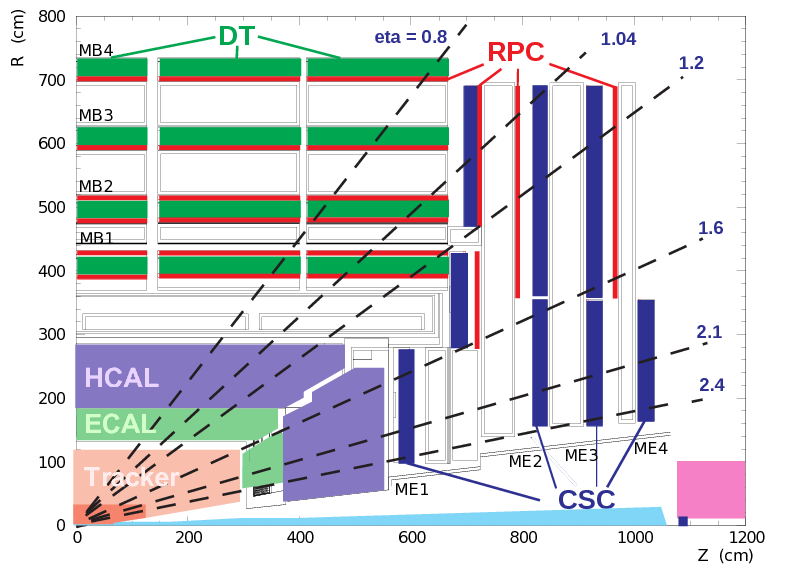
\includegraphics[width=0.65\textwidth]{figures/general/CMS_eta.png}
 \caption{A sketch of one quadrant of the CMS detector is shown with the main detector components~\cite{CMSEta}.}
 \label{fig:etaPlaneCMSTotal}
\end{figure}

\subsection{Muon system}
The most outside part of the CMS detector is the muon system. Because all other particles besides muons should be stopped in the inner layers, muons are the only particles trespassing and leaving the muon system. Three different types of detectors are used to measure and identify muons. The barrel part ($|\eta|<1.2$) is covered by four stations of drift tubes (DT). Cathode strip chambers (CSC) are covering the endcap at pseudorapidity $0.9<|\eta|<2.4$, because in this region a higher muon rate is expected, and CSCs in contrast to DTs have a faster response time and are more radiation hard. In most of the parts the muon efficiency is above $95\%$, with the misidentification is less than $1\%$. The muon momentum resolution, dependent on the $\eta$ region, varies between $1\%$ to $6\%$ for muons with a transverse momentum below $100\GeV$, and is in the order of $10\%$ for $\TeV$ muons~\cite{MuonPerformance}.\\
Additional deetctor components, namely six layers of resistive plate chambers (RPC), are installed in the pseudorapidity range of $<\eta|<1.6$. Because they show both good time resolution and fast response time, they are mainly used for triggering purposes. The structure of the muon system can be seen in \refFig{fig:etaPlaneCMSTotal}.

\subsection{Trigger system}
As collisions take place every $25\ns$, and therefore at a rate of $40\MHz$, it is not achievable to read out and store all event details. To keep only physically interesting events and reduce the rate of events to be saved, a trigger system consisting of two stages is implemented~\cite{TriggerSystem}. It is composed of the hardware based level 1 triggers (L1), and the software based high level triggers (HLT). Since the L1 trigger needs to deliver decisions in a very short time window, it uses only information provided by the calorimeters and the muon chambers. Usually first requirements on the event, such as a minimal deposited transverse energy, and  the presence of first estimates for electron and muon candidates, are imposed. The L1 trigger reduces the event to a rate of $\approx100\kHz$.\\
A more complex decision taking is performed by the HLT trigger system. It has full access to the total readout of all subdetectors, and therefore performs selections close to the offline analysis. It reduces the event rate to $\mathcal{O}(400\Hertz)$.\\
Using the decisions of the HLT, events are categorized into different subsets, based on event kinematics and the trigger objects.

\chapter{Simulation, data processing, and event reconstruction}\label{chap:reco}
The data sets, based on the proton-proton (pp) collisions and recorded with the CMS detector, are centrally provided in the \texttt{MINIAOD} format~\cite{MiniAOD}. This format contains only parts of the original event and detector information relevant for most of the physics analyzes. An analysis looking for deviations from expectations from the SM is supposed not to be biased while development. Thus, SM and signal Monte-Carlo (MC) simulations are performed and are centrally provided by the CMS collaboration. These are also provided in the \texttt{MINIAOD} format with extended generator informations.\\
All available data sets, including measured data and simulation, are further processed with the help of the CMS software framework (CMSSW\footnote{Version 8.0.26})~\cite{CMSSW}, the CMS Remote Analysis Builder (CRAB3)~\cite{CRAB}, and the ressources of the Worldwide LHC Computing Grid (WLCG)~\cite{Grid}, to obtain files with significantly reduced size. The obtained reduced information is stored in the \texttt{ROOT}~\cite{ROOT} file format, and can be used by analysists with self-developed software~\footnote{Usually composed of parts developed in \texttt{C/C++} and \texttt{Python}}.\\
\\
In this chapter, at first the used data samples are introduced. Thereafter, an overview on MC simulation is given, while the simulated samples used in this analysis are reviewed. After that, the event reconstruction performed on all data sets is explained. A more detailed view is given on the reconstruction and identification of physics objects.\\
Protons are very complicated objects composed of many different quarks and gluons. The probability to find a distinct parton of a proton in a deep-inelastic-scattering is given by Parton distribution functions (PDFs) and the underlying parton density functions~\cite{PDF}. Hence, an event measured with the CMS detector is not clean, but shows different effects. The interaction between the colliding two partons is described as the hard interaction. The products and quantities of these interactions contain the most interesting physical information. But, due to the structure of the proton, many different lower energetic particles can be produced in interactions between additional partons (multi-parton-interactions). These remnants of the scattering process, together with reconstructed remnants of the protons, are denoted as the underlying event. Interactions between protons in the same bunch crossing are referred to as pileup.

\section{Data sets}\label{sec:datasets}
This analysis uses different data sets based on the pp-collisions of the LHC with a center-of-mass energy of $13\TeV$ in 2016 and recorded with the CMS detector, corresponding to an integrated luminosity of $35.9\fbinv$. Each primary data set (PD), is a composition of events recorded with similar HLT trigger paths. The \texttt{DoubleMuon} and \texttt{DoubleEG} PDs are used in the central part of the analysis for the signal selection, since they contain events with two muons or electrons respectively. \texttt{MET} and \texttt{HT} PDs are used for trigger efficiency measurements, and the \texttt{MuonEG} PD is used to extract a selection relevant for the background prediction. For a list of used triggers see \refSec{sec:triggerEff}.\\
The different PDs are separated into several single samples for different run eras troughout 2016. The paths of the used samples with the \texttt{03Feb2017} version of reconstruction available via the CMS data set bookkeeping service (DBS)~\cite{DASBookkeeping} are listed in \refTab{tab:datasets}.
\todo{refs zu chaptern}

\begin{table}[htb]
 \centering
 \caption{Data sets used in the analysis.}
 \label{tab:datasets}
 \begin{tabular}{l|l}
  \hline
  \multirow{5}{*}{PDs}       & DoubleEG               \\
                             & DoubleMu               \\
                             & MuonEG                 \\
                             & HT                     \\
                             & MET                    \\\hline\hline
  \multirow{ 4}{*}{DBS path} & \verb|/PD/Run2016B-03Feb2017_ver2-v2/MINIAOD| \\
                             & \verb|/PD/Run2016(C-G)-03Feb2017-v1/MINIAOD| \\
                             & \verb|/PD/Run2016H-03Feb2017_ver2-v1/MINIAOD| \\
                             & \verb|/PD/Run2016H-03Feb2017_ver3-v1/MINIAOD| \\
  \hline
 \end{tabular}
\end{table}


\section{Simulation}
The simulation process for SM background and SUSY signal samples can be devided in three major steps, which are very similar for both cases. At first, for a specific process events are simulated with an event generator. The event generators used for the generation of the samples considered in this analysis are \MADGRAPH5 in leading order (LO) configuration~\cite{Madgraph1,Madgraph2,Madgraph3}, \MADGRAPH\_\MCATNLO in next-to-leading order (NLO)~\cite{Madgraph1,AMCATNLO}, \PYTHIA~\cite{Pythia} for both cases of accuracy, or \POWHEG~\cite{Powheg1,Powheg2}. Matrix elements for the contributing diagrams are computed, and via convolving with PDFs, cross sections are calculated. These cross sections later can be used to rescale the MC simulation to a given integrated luminosity. Thus, the simulation can be performed with very high statistics and can still be compared to measured data.\\
Depending on the choice of the chosen generator, a separate generator for the simulation of hadronic showers must be used. This is done with \PYTHIA. Therewith partons generated in matrtix element corresponding to the hard interaction, and partons generated with \PYTHIA in the showering for \eg initial state radiation (ISR), are not double counted, a matching with the \textsc{MLM}~\cite{Madgraph2} (LO) or \textsc{FXFX}~\cite{AMCATNLO} (NLO) matching schemes is performed. The hadronization of the partons (quarks and gluons) is simulated also with \PYTHIA, based on the confinement of color charged particles.  This, together with the underlying event and pileup, is all covered by the \textsc{CUETP8M1} generator tune~\cite{Tune}. It is based on $7\TeV$ proton-proton CMS and proton-antiproton CDF measurements. The PDFs used for the generation of the MC samples are provided by the \textsc{NNPDF} 3.0 sets~\cite{NNPDF}.\\
The big next step, which is the most time and ressource consuming part, is the simulation of the detector response. A full model of the CMS detector was contructed with the \GEANTfour~\cite{Geant} package. Hence, it allows a precise simulation of the detector response for the events generated with the procedure described above. In the \GEANTfour package, material and particle properties, detector effects, and decay structures are considered in the simulation process. Since this procedure is very time consuming, but leads to a high accuracy, a different method is chosen for processes, whose description is limited by different aspects. So for the generation of SUSY samples, where theoretical uncertainties dominate, the CMS \textsc{FASTSIM} packages is used~\cite{FastSim}. It is based on a siplified geometry and parametrizations, yielding a reduction in runtime of the factor $\approx100$. If the "FullSim" and "FastSim" performances are compared~\cite{FastSimQuality}, a agreement within $\approx10\%$ is observed.\\
\\
All MC simulated processes used in this analysis are listed in \refTab{tab:MCsamples} together with their corresponding cross sections used to rescale the samples later on. The DBS paths are given in the appendix.\todo{ref}\\

\begin{table}[htb]
 \centering
 \caption{All SM model simulated samples used in the analysis with their cross sections. For their corresponding accuracy refer to the text. Additional k-factors to obtain NNLO cross sections for the $\PZ\PZ$ samples are applied per event in dependence of the $\pt$ of the diboson system. All samples are of the \texttt{MINIAODSIM} format.}
 % \scriptsize
 \label{tab:MCsamples}
 \begin{tabular}[width=\textwidth]{ll|ll}
  \hline
  \normalsize{process}                             & \normalsize{$\sigma\,[\mathrm{pb}]$} & \normalsize{process}                         & \normalsize{$\sigma\,[\mathrm{pb}]$} \\\hline
  \scriptsize{\textbf{ttbar}}                      &                                      & \scriptsize{\textbf{diboson}}                &                                      \\
  $\ttbar\to\ell^{+}\PGn\cPqb+\ell^{-}\PAGn\cPaqb$ & $87.31$                              & $\PZ\PGg\to2\ell\PGg$ ($\pt^{\PGg}<130\GeV$) & $124.936$                            \\
  \scriptsize{\textbf{ttbarGamma}}                 &                                      & $\PZ\PGg\to2\ell\PGg$ ($\pt^{\PGg}>130\GeV$) & $0.1488$                             \\
  $\ttbar\PGg\to2\ell2\PGn2\cPqb\PGg$              & $1.679$                              & $\PW\PZ$                                     & $4.9125$                             \\
  $\ttbar\PGg\to4\PQq2\cPqb\PGg$                   & $3.482$                              & $\PZ\PZ\to2\ell2\PGn$                        & $0.5644\cdot k(\pt^{ZZ})$            \\
  $\ttbar\PGg\to\ell\PGn2\cPqb2\PQq\PGg$           & $2.509$                              & $\PZ\PZ\to2\ell2\PGn$                        & $0.5644\cdot k(\pt^{ZZ})$            \\
  \scriptsize{\textbf{DrellYan}}                   &                                      & $\PW\PW\to2\ell2\PGn$                        & $12.178$                             \\
  $\PZ/\PGg^{*}\to2\ell$                           & $5765.4$                             & $\PW\Pg\to\ell\PGn\PGg$                      & $489$                                \\
  \textbf{single top}                              &                                      & \textbf{W jets}                              &                                      \\
  $\PWp\to\cPqt\cPaqb$                             & $3.36$                               & $\PW+jets$                                   & $61526.7$                            \\
  $\cPq\cPaqb\to\cPq^{'}\cPaqt$                    & $80.95$                              & \textbf{triboson}                            &                                      \\
  $\cPq\cPqb\to\cPq^{'}\cPqt$                      & $136.02$                             & $\PW\PW\PGg$                                 & $0.2147$                             \\
  $\cPaqb\to\PWp\cPaqt$                            & $11.7$                               & $\PW\PZ\PGg$                                 & $0.04123$                            \\
  $\cPqb\to\PWm\cPqt$                              & $11.7$                               &                                              &                                      \\
  \hline
 \end{tabular}
\end{table}



The Drell-Yan (DY) $\PZ/\PGg$ process, as well as the diboson $\PZ\PGg$ and $\PW\PGg$ processes, and triboson production of $\PW\PW\PGg$ and $\PW\PZ\PGg$ are generated with \MADGRAPH\_\MCATNLO in NLO. Top pair production in association with a photon ($\ttbar\PGg$) and the production of a $\PW$ boson in association with jets are also simulated using the \MADGRAPH\_\MCATNLO generator in NLO. Top pair production with leptonic decays ($\ttbar\to 2\ell 2\PGn 2\cPqb$), diboson production of $\PW\PZ$, $\PZ\PZ$, $\PW\PW$, and all singletop production processes are generated using \POWHEG.
The diboson $\PW\PW$ and $\PW\PGg$ production, the production of $\PW+jets$, triboson $\PW\PW\PGg$ and $\PW\PZ\PGg$ production, and all singletop production channels are grouped together and denoted as "other" in the following.
Next-to-leading order and next-to-next-to-leading order (NNLO) cross sections~\cite{xsec1,xsec2,xsec3,xsec4,xsec5,xsec6,xsec7,xsec8,xsec9} are used for the normaliziation of the samples.\\
The generator used for the signal simulation production is \MADGRAPH\_\MCATNLO for the simplified models, and \PYTHIA8 for the full GGM model. The corresponding DBS paths are also listed in the appendix\todo{ref}.
The cross sections used in the signal normalization are calculated at NLO accuracy for the full GGM scenario, and at NLO+next-to-leading logarithmic (NLL) accuracy for the two simplified models~\cite{sxsec1,sxsec2,sxsec3,sxsec4,sxsec5,sxsec6,sxsec7,sxsec8,sxsec9}.
For the electroweak SMS the applied cross section is calculcated for $\charginoOne\neutralinoOne$ and $\charginoOne\charginoOneBar$ production with squarks and gluinos decoupled, and the sum of both is used. In the cross section calculation of gluino pair production for the other SMS squark decoupling is assumed. The applied cross sections for the GGM scenario are obtained using a full model, thus beeing different from the ones used for the electroweak SMS.\\
For the GGM model signal points are generated with wino masses ranging from $215\GeV$ to $1015\GeV$, and bino masses from $205\GeV$ to $m(\widetilde{W})-10\GeV$ in intervals of $25\GeV$.
In case of the \texttt{TChiZG} SMS, points are generated with NLSP masses in the range of $300-1300\GeV$ in steps of $25\GeV$. The grid of points generated for the \texttt{T5bbbbZG} strong production SMS includes gluino masses in the range of $800\GeV$ to $2500\GeV$, while the NLSP massrange is scanned from $10\GeV$ to $m(\widetilde{g}-10\GeV$ in non equidistant steps.\\
\\
As mentioned above, the true number of generated MC events $N_{Gen}$ is very high. Thus, together with the measured integrated luminosity $\Lumi$, and a given cross section $\sigma$, a global event weight of
\begin{equation}
 w = \frac{\Lumi \cdot \sigma}{N_{Gen}}
\end{equation}
is obtained.\\
Additional event weights are applied on the simulation to account for differences in the pileuip distribution. To improve on the \MADGRAPH modeling of the multiplicity of additonal jets arising from initial state radiation, SUSY SMS MC events are reweighted as a function of $N^{ISR}_{Jet}$ or the transverse momentum of the ISR system, to improve the agreement with observations in data.
The latter is based on studies of the transverse momentum of $\PZ$ events.~\cite{NISRweight}.
The differences to 1 for the reweighting factor is considered as a systematic uncertainty later on.
The \POWHEG \ttbar simulation is also reweighted as a function of the transverse momentum of the top system, based on studies in top pair production cross section measurements~\cite{topWeight1,topWeight2,topWeight3,topWeight4} to improve the agreement of the transverse momentum of the top quark with data.

\subsection{Overlap Removal}
Because samples are used for processes, such as top pair production and Drell-Yan, for the nominal process and additional photon production in the hard interaction, there exists an overlap between those simulated samples. This is the case, since the photon production in the hard interaction is physically the same, as \eg photon radiation in the initial state. Hence, this overlap needs to be removed. Therefore, events that show a signature like the one simulated in the exclusive hard photon interaction samples, are removed on generator level from the nominal MC samples. So after the apllying of the removal procedure both samples can be added, and double counting of diagram contributions is rejected.

\section{Event and particle reconstruction and identification}
To maintain both, a precise and robust particle reconstruction, and flexibility in the physical object identification, particle reconstruction and identification is divided in two major parts. At first, particles and their properties, such as momentum, energy, and trajectory, are reconstructed with the Particle Flow (PF) algorithm~\cite{ParticleFlow} by combining informations from all CMS subdetectors. After that, identification criteria determined by specialized CMS physics objects groups (POGs) are applied, dependent on the choice of the analyst regarding efficiency and misidentification rates.\\
In the following the PF algorithm is briefly introduced by explaining its main features, and more detailed definitions of the physical objects are given.

\subsection{Particle Flow}
Particles are reconstructed and categorized by PF in five classes, namely muons, electrons, photons, and both neutral and charged hadrons. The decisions are made based on two major reconstruction steps, finding and reconstructing tracks of charged particles, and separate clustering of ECAL and HCAL entries, to reconstruct the energy deposit of the particles' showers.\\
The track finding algorithm based on Kalman filtering~\cite{Kalman} iteratively generates seeds for the tracks, builds trajectories, and performs a final fit to determine the particle properties, such as direction and momentum based on information of the inner tracker.
For particles, such as muons and electrons, additional tracking algorithms are used, to determine a more accurate description of the particle's properties. For muons, additional information of the muon system is used to directly classify three types of non exclusive muon tracks. Standalone muon tracks are reconstructed using only informations of the muon system. If inner tracker tracks can be matched to entries in the muon system, they are called tracker muon track. And in cases where muon system tracks are matched to inner tracks, these are called global muon tracks.
For electrons additional fitting procedures combining tracker and ECAL informations are used to cope the characteristics of the electromagnetic showers~\cite{GSFTrack}. Therefore, superclusters are built within the ECAL by combining nearby clusters, and the seeds determined with the tracker based pproach described above, together with this ECAL based reconstructed seeds, are used in a common track fit.\\
The clustering algorithm for the ECAL and HCAL also at first determines cluster seeds based on local energy maxima, and afterwards adds cluster entries fulfilling certain energy criteria to obtain topological clusters.\\
The following combination and linking of the determined information is motivated by the main characteristics of the particle interactions:\\
Photons are neutral particles, and therefore they leave no track in the detector, but only interact electromagnetic. Thus, they are stopped in the ECAL by generating electromagnetic showers. They can also undergo electron-positron pair production, resulting also in an electromagnetic shower in the ECAL.\\
Electrons are charged particles. Hence, their tracks are reconstructable in the tracker, and the energy deposit happens also via electromagnetic shower generation due to Bremsstrahlung in the ECAL. Accordingly, electrons and photons are very similar objects in the reconstruction procedure.\\
Muons are mainly identified by the informations of the muon system, since no other particles except for very high energetic jets punching through the solenoid and outer HCAL, are capable of reaching the muon chambers. By combining the inner tracks with the entries of the muon chambers, a clear and precise muon identification is maintained.\\
Charged and neutral hadrons are reconstructed by clusters in the HCAL, and can be differitiated by corresponding matching tracks in the tracker. Part of non-promt photons, \eg coming from meson decays, are also reconstructed as neutral hadrons.\\
The order of particle reconstruction is based on the accuarcy and precision of the available information. Thus, muons are identified first, followed by electrons and prompt photons. After that, neutral and charged hadrons, and non-prompt photons are identified.\\
All these informations obtained by the PF algorithm, provide the basis for the final physical object identification applied by the analysts.

\subsection{Primary vertex}
The primary vertex is defined by the vertex with the largest sum of transverse momenta determined by vertex reconstruction algorithms~\cite{vertex}, and needs to be reconstructed within a distance of $24\cm$ in z direction, and $2\cm$ in the x-y-plane.


\subsection{Muons}
Muons are required to have a transverse momentum larger than $15\GeV$. And because the muon chambers extend only to a pseudorapidity range of $|\eta|<2.4$, muons need to be reconstructed within this region. In addition, muons have to pass a some quality requirements obtained by the muon POG, yielding a $\approx 98\%$ efficiency~\cite{MuonIDPerf}.\\
The muon needs to be reconstructed as a PF muon, and either as a global muon or a tracker muon. If it is reconstructed as a global and a tracker muon, the segment compability, which is a measure for the compability between the tracker tracks and an extrapolation to the muon system, has to be larger than $0.303$. In addition, more than $80\%$ of the inner track layers need to be used within the track fit, the normalized goodness of fit ($\chi^2/ndof$) needs to be less than $3$, the match between the standalone muon position and the tracker muon must have $\chi^2<12$, and the maximum $\chi^2$ found by a kink finding algorithm, which tries to seperate the track into two independent tracks, needs to be smaller than $20$. If the muon is reconstructed exclusivley as a tracker muon, only the segment compability needs to be greater than $0.451$, and the other requirements on the track quality are removed.\\
Besides the identification requirements, conditions on the position of the track relative to the reconstructed primary vertex are imposed. In the transversal direction ($d_{xy}$), muon tracks need to be closer than $0.05\cm$ to the vertex, and in the longitudinal direction ($d_z$), the distance needs to be smaller than $0.1\cm$. A cone dependent isolation is introduced, called "mini isolation", where the cone size in the $\phi-\eta$ plane is calculated relative to the transverse momentum of the particle as follows:
\begin{equation}
 R = max\left(0.05,min\left(0.2,\frac{10\GeV}{\pt}\right)\right).
\end{equation}
Pile up corrections are also taken into account in the mini isolation calculation.
The determined energy deposit in the cone around the muon must not exceed $10\%$ of the transverse momentum of the particle.


% \begin{table}[h!]
%  \caption{\todo{caption}}
%  \label{tab:muonID}
%  \centering
%  \begin{tabular}{ll}
%   variable                                            & requirement \\\hline
%   global muon                                         & true        \\
%   fraction of valid inner tracker hits                & $>0.8$      \\
%   normalized $\chi^2$ of global track                 & $<3$        \\
%   chi2localposition (track standalone position match) & $<12$       \\
%   kink finder                                         & $<20$       \\
%   segment compability                                 & $>0.451$
%  \end{tabular}
% \end{table}



\subsection{Electrons}
The list of requirements imposed on the electron selection is driven by a symmetric approach between the two lepton selections. The same conditions on the distance to the primary vertex, ($d_{xy}<0.05$, $d_z<0.1$), the maximum pseudorapidity ($|\eta|<2.4$), and transverse momentum ($\pt>15\GeV$) need to be fulfilled. The mini isolation criterion is relaxed to $20\%$.\\
The identification requirements determined by the EGamma POG~\cite{ElectronID} seperately for electrons reconstructed in the ECAL barrel (EB: $|\eta_{Supercluster}|<1.479$) and endcap (EE: $|\eta_{Supercluster}|>1.479$) region are listed in \refTab{tab:eleID}.
\begin{table}[h!]
 \centering
 \caption{\todo{cap}}
 \label{tab:eleID}
 \begin{tabular}{lcc}
  Variable                       & \multicolumn{2}{c}{Value}              \\\hline
                                 & EB                        & EE         \\\hline
  $\sigma_{i\eta i\eta}$         & $<0.00988$                & $<0.0298$  \\
  $\Delta\eta_{Seed}$            & $<0.00311$                & $<0.00609$ \\
  $\Delta\phi_{In}$              & $<0.00311$                & $<0.00609$ \\
  $H/E$                          & $<0.253$                  & $0.0878$   \\
  relative combined PF isolation & $<0.0695$                 & $<0.0821$  \\
  $|\frac{1}{E}-\frac{1}{p}|$    & $<0.134$                  & $<0.13$    \\
  \# missing inner hits          & $\leq1$                   & $\leq1$    \\
  Photon conversion veto         & true                      & true       \\\hline
 \end{tabular}
\end{table}
Here, $\sigma_{i\eta i\eta}$ is a quantity characterizing the width of the electromagnetic shower shape in the ECAL in the $\eta$ direction. It is calculated as a weighted variance of energy deposits in the full 5x5 pixel ECAL supercluster. Since jets emerging from hadrons have a wider shower in the ECAL than electrons, a differentiation can be achieved. Consistency between the informations of the reconstructed track at the vertex, and the supercluster is required, by setting conditions on $\Delta\eta$, $\Delta\phi$, and the supercluster energy $E$, and track momentum $p$. To further separate electrons from hadrons, more energy should be deposited in the ECAL, rather than in the HCAL ($H/E$). An isolation requirement based on the PF determined isolation, assures that prompt electrons are seperated from electrons coming from \eg jets. Contributions from photons faking electron signatures are suppressed, by imposing a requirement on the number of missing inner hits in the tracker, and an additonal veto for photon conversions to electron-positron pairs determined in an $\chi^2$ fit.

\subsection{Photons}
Photons need to have a transverse momentum larger than $20\GeV$. Because photons are produced more centrally due to the high masses and short lifetimes in the considered SUSY signal scenarios, only photons reconstructed in the ECAL barrel are considered ($|\eta<1.4442|$). Additional identification criteria determined by the EGamma POG~\cite{photonID} are listed in \refTab{tab:photonID}.
\begin{table}[h!]
 \centering
 \caption{\todo{cap}}
 \label{tab:photonID}
 \begin{tabular}{lc}
  Variable                    & Value                                                \\\hline
  $\sigma_{i\eta i\eta}$      & $<0.01031$                                           \\
  $H/E$                       & $<0.0597$                                            \\
  PF charged hadron isolation & $<1.295$                                             \\
  PF neutral hadron isolation & $<10.910 + 0.0148 \cdot \pt + 0.000017\cdot (\pt)^2$ \\
  PF photon isolation         & $<3.630+0.0047\cdot \pt$                             \\\hline
 \end{tabular}
\end{table}
Similar to the requirements on $\sigma_{i\eta i\eta}$ and $H/E$ for the electron selection, these conditions in the photon identification ensure the suppression of selecting hadrons faking the photon signature. Additional different isolation criteria lower the amount of selected photons originating from neutral and charged hadrons, and photons coming from light meson decays.\\
Requirements on the distance in the $\eta-\phi$ plane between the photon and selected lepton candidates ($\Delta R(\PGg,\ell)>0.3$) significantly reduce contributions from final state radiation (FSR) photons. By requiring that no pixel seed can be assigned to a trajectory between ECAL supercluster and interaction point, a clear differentiation between electrons and photons is achieved.

\subsection{Jets}
Jets, see \refSec{sec:SM}, are very complicated objects due to the complexity of the hadronization and fragmentation processes. Therefore, a a sophisticated clustering algorithm is needed to measure the energy of jets properly. Jets are clustered with the anti-$k_T$ algorithm~\cite{AntiKT} included in the \FASTJET package~\cite{FastJet1,FastJet2} with a distance paramater of $R=0.4$. The jet momentum is defined as the total sum of the momenta of the constituents of the jet. CHarged hadrons not emerging from the primar vertex are not considered in the clustering. The jet energy is corrected for effects originating from pile up and the detector response, tuned with the help of different data control selections and simulation~\cite{JEC}. Reconstructed jets need to pass a loose ID proposed by the Jet-Missing Transverse Energy POG~\cite{JetID}, need to have a transverse momentum larger than $30\GeV$, and the pseudorapidity must not exceed $|\eta=3|$. In addition, jets overlapping with photon and lepton candidates in a cone with radius $R=0.4$ in the $\eta-\phi$-plane, are removed from the selection to forbid double counting of objects.

\subsection{Missing transverse momentum}
The missing transverse momentum $\ptmiss$ is one of the most important observables in searches for BSM physics. In typical SUSY models, see \refSec{sec:SUSY}, a significant amount of $\ptmiss$ is expected in the events due to the LSP. In SM processes only neutrinos and mismeasurements of \eg the jet energies lead to missing transverse momentum, because before a collision the transverse momentum of the colliding protons is nearly negligible. Hence, the missing transverse momentum quantifies the imbalance of all reconstructed particles in an event and is defined as
\begin{equation}
 \ptmiss= |\ptvecmiss| = |-\sum_{PF objects}\pt_i|.
\end{equation}
Jet energy corrections are propagated to the missing transverse momentum vector to reduce a strong bias in events with large hadronic activity.

\section{Definition of observables}
Throughout this thesis different observables are used to define different phasespace regions, in particular the signal region and control and validation regions important for the background prediction. All these high level variables are defined based on low level quantities such as the $\pt$ of different objects, or are calculated by complex algorithms combining them.

\subsection*{Total hadronic activity $\HT$}
The hadronic activity $\HT$ is defined as the scalar sum of all jets transverse momenta
\begin{equation}
 \HT = \sum_{Jets} |\ptvec_i|
\end{equation}

\subsection*{The transverse mass $m_{T}$}
The transverse mass of two objects with transverse momentum $\ptvec^A$ and $\ptvec^B$ yields the transverse mass of the mother particle if both particle emerge from the saame decay. In cases of invisible decay products, the transverse mass is an estimate of the mother mass in the transverse plane, and therefore a good estimate for the total mother particle mass, because the missing momentum can only be determined in the transverse plane. It is defined as
\begin{equation}
 m_T\left(\ptvec^{A},\ptvec^B\right) = \sqrt{2|\ptvec^A||\ptvec^B|\left(1-\cos(\Delta\phi)\right)},
\end{equation}
where $\Delta\phi$ is the angle between $\ptvec^A$ and $\ptvec^B$ in the transverse plane.

\subsection*{The stransverse mass $\mtTwo$}
In case of two identical particles, decaying both to one invisible and one visible particle, the stransverse mass $\mtTwo$~\cite{Mt2_1,Mt2_2} is a useful generaliziaton of $m_T$. In this analysis it is calculated to estimate the mass of the NLSP, which decays to an invisible object, the gravitino, and one visible particle, a Z boson or a photon. It is defined as
\begin{equation}
 \mtTwo = min_{\ptvec^{\Pgn_1}+\ptvec^{\Pgn_2}=\ptvecmiss}\left(max\left[m_T(\ptvec^{\PZ},\ptvec^{\Pgn_1}),m_T(\ptvec^{\PGg},\ptvec^{\PGn_2})\right]\right),
\end{equation}
where the final value is determined via minimization as indicated by $min$ in the equation. Descriptively, the algorithm tries to estimate the transverse mass of the mother particle under the assumption, that the $\ptmiss$ is composited of exactly two identical particles each from one decay branch.\\
For decays of the NLSP in all signal models, the $\mtTwo$ distribution has a cut-off at the mass of the lightest neutralino, while for all SM backgrounds $\mtTwo$ yields much lower values in comparison to the high SUSY massses.
\todo{Plot einfuegen zur verdeutlichung}
\section{Lepton pair selection and quality requirements}{sec:lepPair}
In the analysis different datasets triggered with different dilepton triggers are combined, see \refSec{sec:datasets}. Therefore it is possible, that an event is contained in more than one dataset. Hence, it is assured with the following procedure, that no event is doublecounted. At first, all leptons per event are sorted by their transverse momenta. Thus, the leading and subleading lepton\footnote{called trailing from now on}, are identified. Their flavor combination then determines the classification of the event as "dielectron", "dimuon", or "electron-muon". For instance, an dielectron event is classified as such, if there a at least two electrons in the event, the event originates from the \texttt{DoubleEG} sample, both the leading and the trailing lepton are electrons, and it is triggered by at least one of the dielectron triggers. This set of conditions ensures the exclusivity of the three selections.\\
In addition, there are some requirements imposed on the dilepton system. The trailing and leading lepton need to be seperated at least by a distance of $\Delta R=0.1$ in the transvse plane, and the invariant dilepton mass $m_{\ell\ell}$ should be larger than $50\GeV$. The first requirement provides a cleaning between the lepton collections, and ensures, that no lepton is counted twice, while the latter threshold is introduced, because the simulation of the Drell-Yan simulation does not include events with lower dilepton masses~\footnote{Events with lower invariant dilepton masses are not of interest for this analysis, since in the following only leptons originating from a Z boson decay are selected, resulting in an invariant dilepton mass around the Z boson mass of $\approx91\GeV$.}.\\
Hereafter, the dielectron and dimuon seelctions are combined to a dilepton selection to increase the statistics in the validation, and especially in the signal region.\\
\\
Also, several event quality filters are applied to reject contaminated events. The list of applied filters is recommended by the POGs~\cite{MetFilter}. It reads:
\begin{itemize}
 \item \texttt{HBHE noise filter}
 \item \texttt{HBHE noise iso filter}
 \item \texttt{ECAL TP filter}
 \item \texttt{eeBadSCFilter}
 \item \texttt{bad PF muon filter}
 \item \texttt{bad charged hadron filter}
 \item \texttt{bad muon filter}
 \item \texttt{beam halo filter}
\end{itemize}
The rejected events consist mainly of events with faulty detector signals, cosmic muons, or muons produced in scattering processes with the beam halo.


\section{Used triggers and trigger efficiency measurement}\label{sec:triggerEff}
As already pointed out in \refSec{sec:datasets}, the events are recorded with various dilepton triggers. For each dilepton combination ($\Pe\Pe,\Pgm\Pgm,\Pe\Pgm$) multiple triggers are used because of the changing instantaneous luminosity over the 2016 run period different triggers were active at different times. The main trigger pathts are isolated dilepton triggers, while non isolated trigger paths are added to increase the efficiency at boosted topologies of the dilepton system. A list of all used HLT trigger paths is given in the appendix in \refTab{tab:}. While the same flavor dilepton triggers ($\Pe\Pe,\Pgm\Pgm$) are used as signal triggers, the different flavor triggers ($\Pe\Pgm$) are used to select events needed for the background prediction of the top pair production ($\ttbar(\PGg)$) background. This will be explained more in detail in \refSec{sec:ttbar}. The dilepton triggers alltogether have transverse momentum thresholds for the dileptons of around $17-33\GeV$ for the leading lepton, and $8-33\GeV$ for the trailing one. Additional triggers with hadronic activity ($\HT$) or $\ptmiss$ thresholds are relevant for the trigger effiency measurement, which will be presented in the following.
\subsection{Trigger efficiency measurement}
A trigger efficiency curve is characterized by a inefficient part, a more or less sharp transition ("Turn On") to the efficient part ideally located at the nominal threshold of the trigger path, and a flat efficient part called plateau.\\
Hence, measuring the trigger efficiency is essential to obtain appropriate transverse momentum requirements for the dilepton system. Furthermore, in the signal MC simulation ussing the \FASTSIM package no trigger simulation is performed like for the SM background samples. Therefore, the efficiency needs to be measured also on simulation, such that the signal simulation can be scaled accordingly. In addition, the SM simulation samples will be weighted with a further event factor, correcting differences in the effiency between data and simulation.\\
As indicated, not a single signal trigger or a single trigger for the control region selection is used, but a logical \texttt{OR} combination of all dilepton triggers with same flavor requirements is used. Thus, for an event only one of the used triggers has to be fired to be selected for the key analysis. Because the total number of produced events, including triggered and non triggered events, in CMS is not available apparantly, for data\footnote{For simulation these informations are available. This is used for further checks to validate the procedure of effiency measurement.}, the combined trigger effiency $\varepsilon$ is measured using a baseline trigger. Thus, it is defined as the number of events passing baseline and signal trigger, divided be the number of events passing only the baseline trigger:
\begin{equation}
 \varepsilon=\frac{\#(baseline \wedge signal)}{baseline}
\end{equation}
As a consequence, the contribution of the baseline trigger cancels, and the pure signal trigger effiency is maintained. As baseline triggers, as mentioned above, a combination of various triggers with $\HT$ thresholds is used. These thresholds range from $200-800\GeV$. Therefore, the measurement is not performed on the dilepton data streams, but on the $\HT$ datasets. The event selection consists basically of the lepton pair selection introduced in \refSec{sec:lepPair} with an additional $\HT>200\GeV$ requirement to ensure, that the baseline triggers are fully efficient. An additional matching between the selected leptons and the trigger objects responsible for the firing of the trigger is performed. Resulting efficiency curves for all three dilepton combinations measured both on data and simulation are shown in \refFig{fig:triggEff} against the $\pt$ of the trailing lepton. The statistical uncertainties of the individual bins are calculated using $95\%$ confidence level (CL) Clopper-Peason intervals~\cite{ClopperPearson}. The measurements suffer mainly from statistics on data, while the statistics of the simulation is very high as expected. The electron-muon channel is affected the most by this effect. However, the efficiency curves show the structure of multiple Turn Ons, as it is expected from a combination of triggers with very different ranges of thresholds. As indicated by the dotted lines in the plots, the lepton $\pt$ cut was determined to be $20\GeV$ for the trailing lepton, and $25\GeV$ for the leading one. Although the dielectron and electron-muon triggers are not yet fully efficient at this threshold as it is the case for the dimuon trigger, this requirement is imposed also on the other to selections in order to obtain a symmetric lepton selection. The mean plateau efficiencies are shown as a gray band with its statistical uncertainty in the plots. The mean efficiency is also measured on simulation, and all values are given in \refTab{tab:triggEff}.
\begin{figure}[htb]
 \centering
 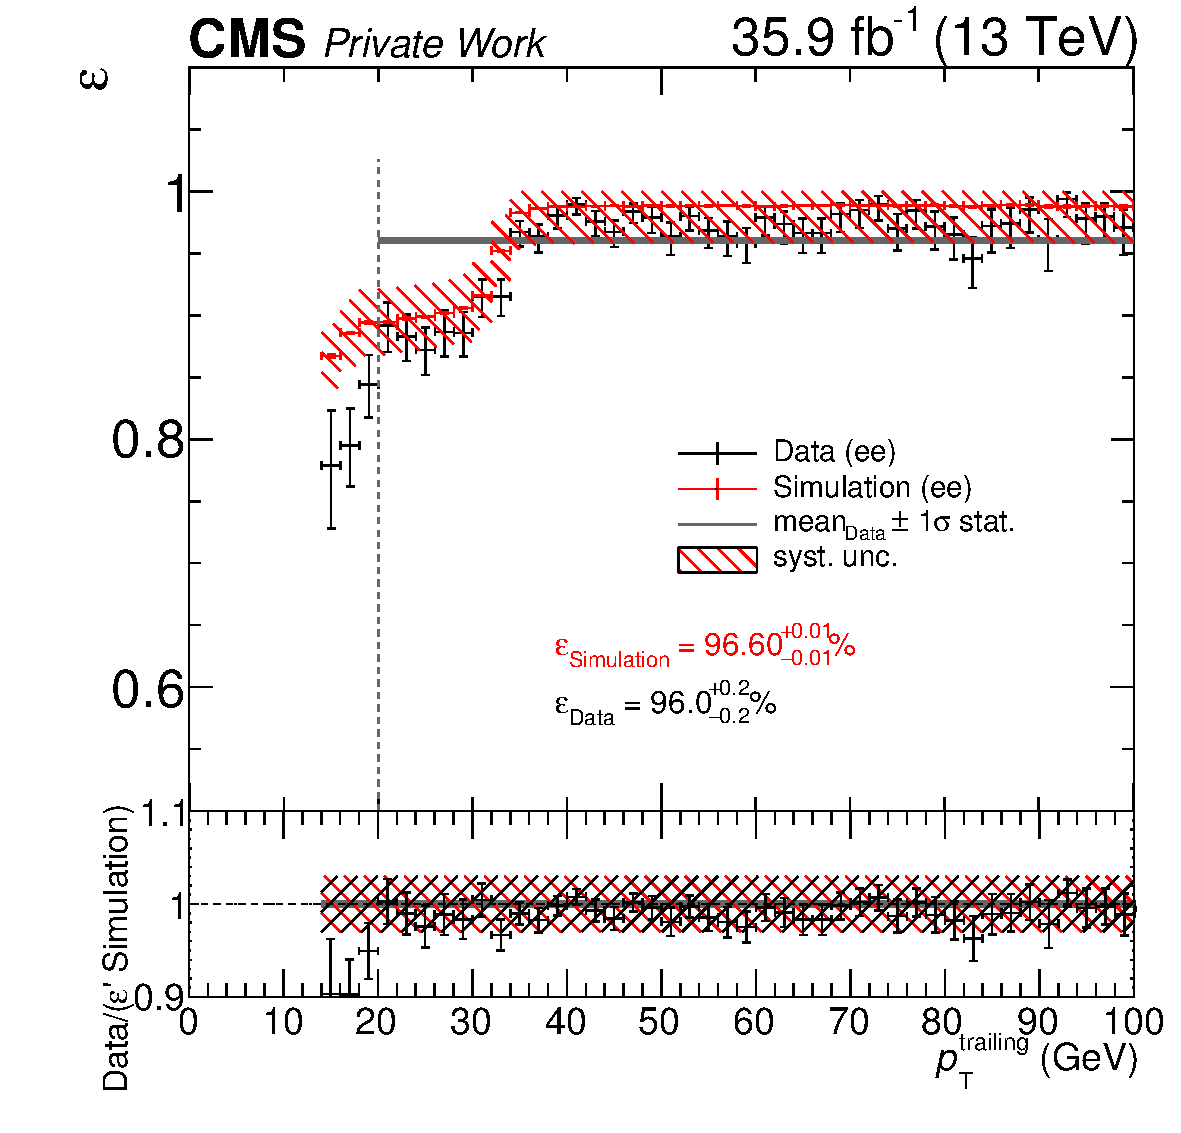
\includegraphics[width=\pairwidth]{figures/triggerStudies/efficiency_dataHT_trigDilep_EE_pt2}
 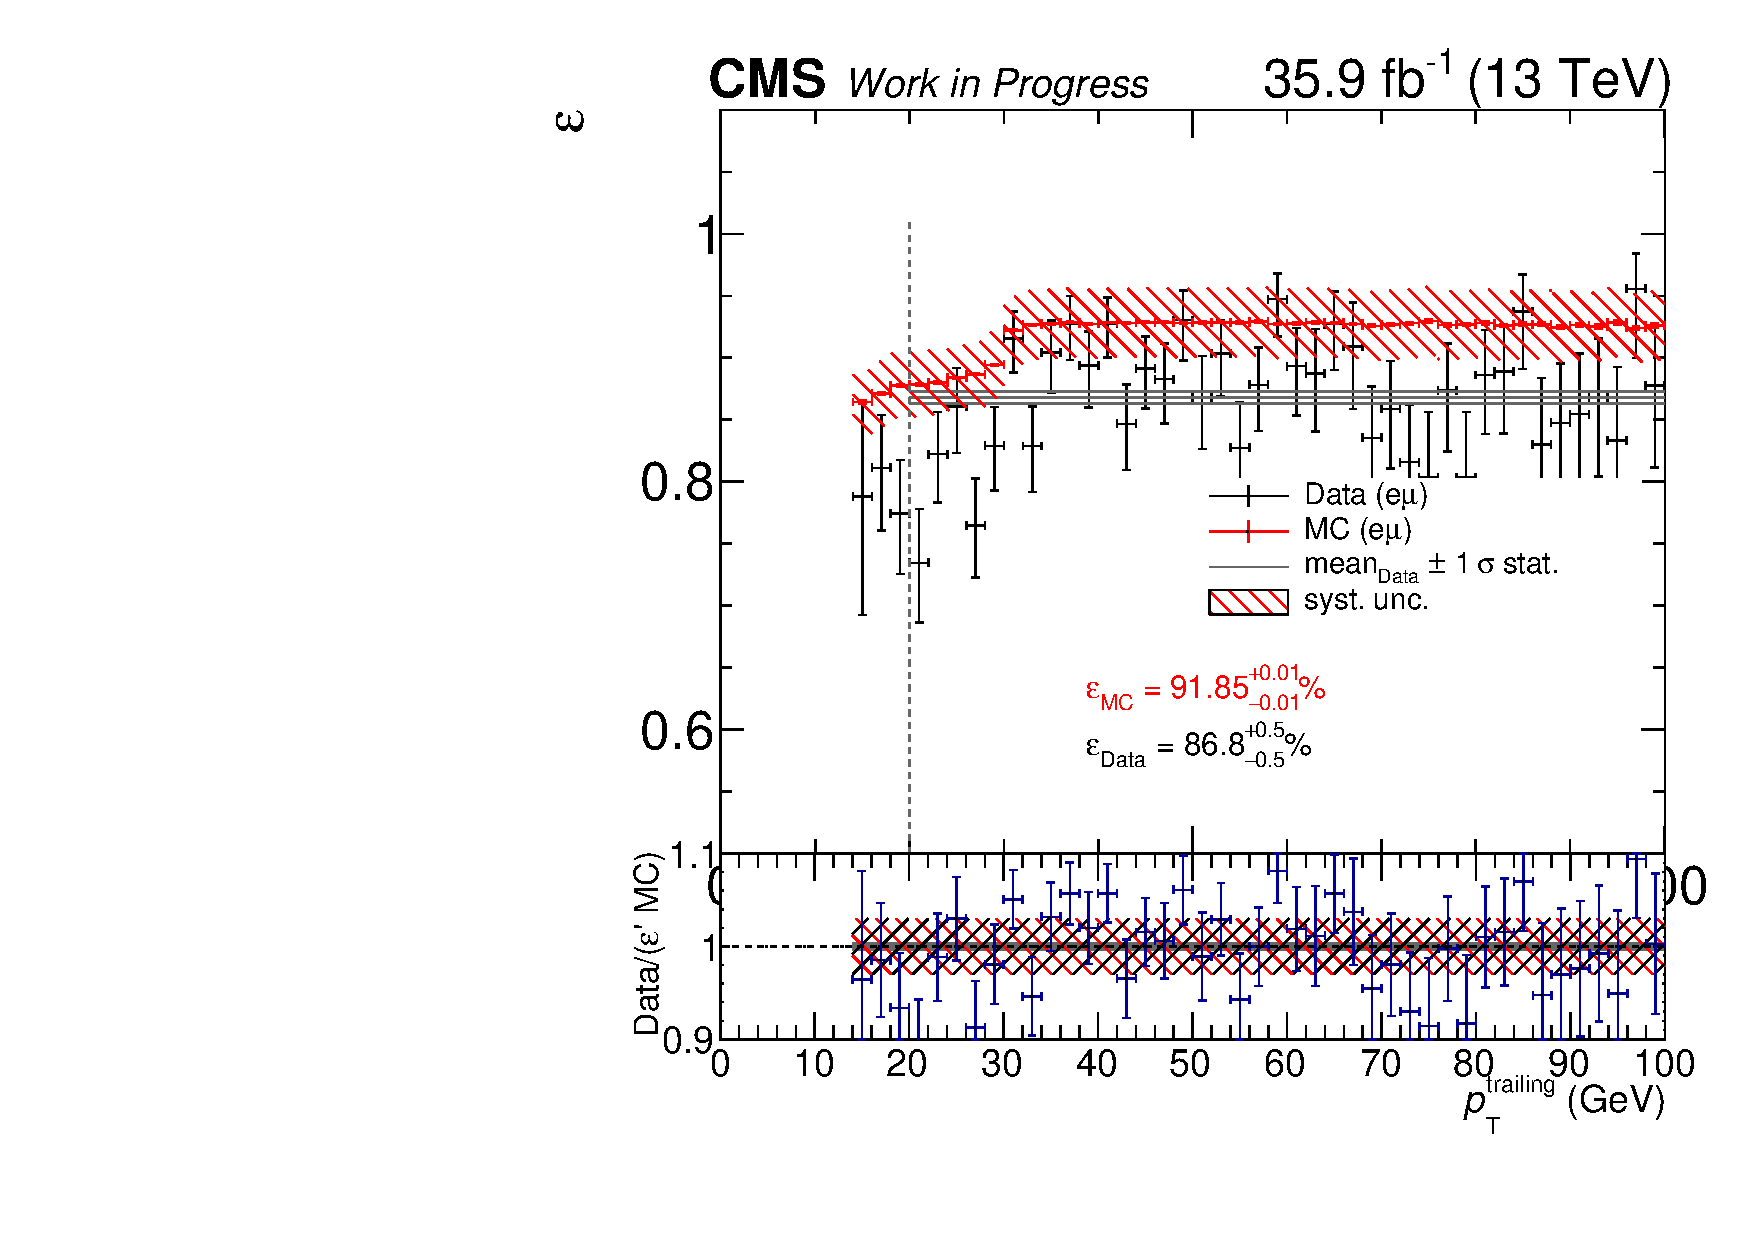
\includegraphics[width=\pairwidth]{figures/triggerStudies/efficiency_dataHT_trigDilep_EM_pt2}
 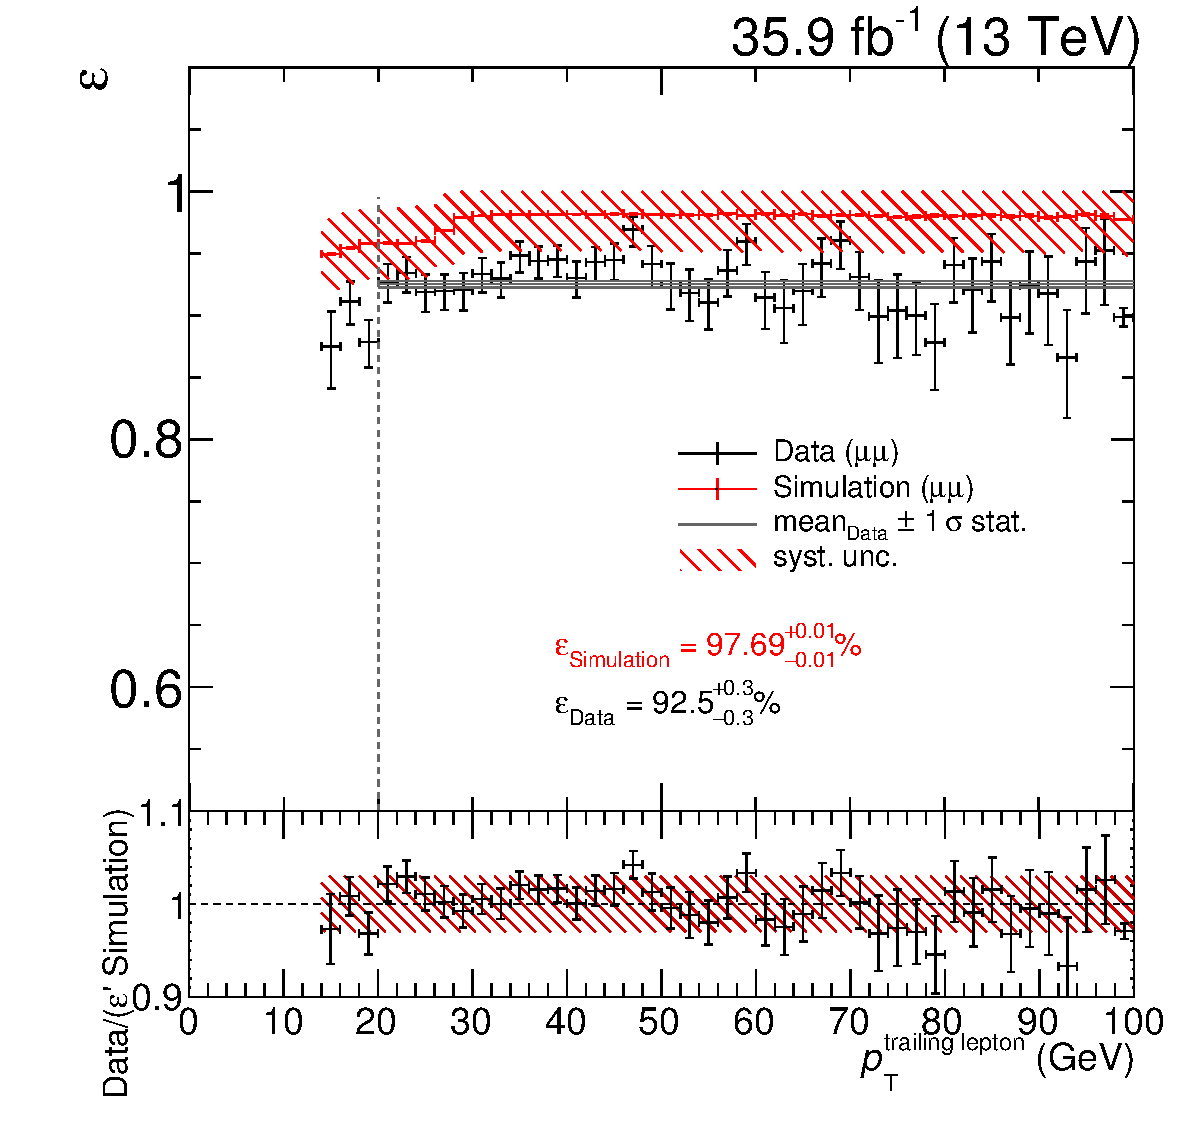
\includegraphics[width=\pairwidth]{figures/triggerStudies/efficiency_dataHT_trigDilep_MM_pt2}
 \caption{\todo{cap}cap}
 \label{fig:triggEff}
\end{figure}


\begin{table}[htb]
 \centering
 \caption{My caption}
 \label{tab:triggEff}
 \begin{tabular}{lllll}
                   & \multicolumn{2}{c}{Data} & \multicolumn{2}{c}{Simulation}                                   \\\hline
  baseline trigger & $\HT$                       & $\ptmiss$                            & $\HT$                        & $\ptmiss$ \\\hline
  $\Pe\Pe$         & $96.0^{+0.2}_{-0.2}\%$   & $93.7^{+0.3}_{-0.3}\%$         & $96.60^{+0.01}_{-0.01}\%$ & $96.79^{+0.02}_{-0.02}\%$   \\
  $\Pe\Pgm$        & $86.6^{+0.5}_{-0.5}\%$   & $86.7^{+0.3}_{-0.3}\%$         & $91.85^{+0.01}_{-0.01}\%$ & $91.34^{+0.05}_{-0.05}\%$   \\
  $\Pgm\Pgm$       & $92.5^{+0.3}_{-0.3}\%$   & $93.9^{+0.3}_{-0.3}\%$         & $91.85^{+0.01}_{-0.01}\%$ & $97.62^{+0.02}_{-0.02}\%$   \\\hline
 \end{tabular}
\end{table}


In addition, in the ratio plots beneath the efficiency curves, the agreement between rescaled simulation with the factor $\varepsilon'=\varepsilon_{Data}/\varepsilon_{MC}$ and data is shown. It can be concluded, that the efficiency measurement works fine for both data and simulation, and the efficiencies agree within the systematic uncertainties, which is determined to be $3\%$ to account for the differences between simulation and data. This is also shown as the red uncertainty band in the plots.\\
As an additional independent check, the whole trigger efficiency measurement was performed on $\ptmiss$ datasets with $\ptmiss$ baseline triggers with thresholds of $110-600\GeV$. This selected phasespace region should be more or less orthogonal the the $\HT$ selection, and is much closer to the final signal region, since the signal regeion selection will contain a $\ptmiss$ threshold, see \refSec{sec:SRSelection}. As can be read from \refTab{tab:triggEff}, the values obtained from this method are also in agreement with the efficiencies measured using the $\HT$ selection.

%
\chapter{Analysis strategy and background estimation}\label{chap:analysis}
\minitoc
Processes producing SUSY particles have significantly smaller cross sections than most SM processes. Therefore, a sophisticated understanding of the relevant production and decay scenarios is needed in order to separate the potential interesting events from the huge amount of SM background. Since this search is targeting SUSY scenarios with bino- and wino-like NLSPs, final states with photons and Z bosons are expected. Choosing the dileptonic decay of the Z boson, there are not many SM background processes leading to the investigated final state. Especially the additional requirement of a photon and $\ptmiss$ in the events reduces most of the background, such that, \eg, the QCD background becomes negligible. Left over are processes producing two same-flavor opposite-charge (SFOC) leptons, one photon and missing transverse momentum. The most important ones are $\ttbar(\PGg)$ production, the combination of Drell-Yan $\PZ/\PGg^{*}$ and $\PZ\PGg$ production, called Drell-Yan/$\PZ(\PGg)$ from now on, $\PZ\PZ$, and $\PW\PZ$ diboson production. This will be discussed in more detail in \refSec{sec:BKG}.\\
The key strategy of this analysis is to impose as little requirements as necessary, to obtain an event selection, so that many model scenarios can be investigated. Hence, only the existence of all expected final state particles is required, where the Z boson is reconstructed from the two selected leptons. Therefore, loose requirements on the lepton and photon energies can be imposed. Not many additional requirements are needed in the following to obtain a sensitive signal region selection.
% \\
% In the final selection a counting experiment is performed, where predicted and observed data yields are compared, and the result is interpreted in different signal models.

\section{Event Selection}
In this section, the event selection is discussed, including region definitions important for the background prediction, which is based on simulation. In those control regions, each enriched with a specific type of background events and suppressed signal contribution, the simulation is tuned to match the measured data. In an additional validation region, the background prediction will be examined, and finally a two bin counting experiment is performed in the signal region.
\subsection{Preselection}
The preselection acts as a first rough definition of the phase space that is of interest, and rejects inefficient parts of the used triggers. The preselection imposed on the dilepton triggered events is defined as follows:
\begin{itemize}
 \item exactly one SFOC lepton pair ($\Pe\Pe$ or $\PGm\PGm$) as defined in \refSec{sec:reco},
 \item $\pt>25\GeV$ for the leading lepton,
 \item $\pt>20\GeV$ for the trailing lepton,
 \item at least one photon,
 \item $\Delta R(\ell_1,\PGg)>0.3$ and $\Delta R(\ell_2,\PGg)>0.3$,
 \item $81\GeV<m_{\ell\ell}<101\GeV$.
\end{itemize}
The first four conditions imply the existence of the final state particles, including the definition of the physics objects and lepton pair selection explained above, and the $\pt$ requirements determined in the trigger efficiency measurement. The fifth requirement reduces contributions of FSR photons. The invariant dilepton mass requirement ensures that only lepton pairs are selected, that originate from an on-shell Z boson decay, and reduces different contributions of SM backgrounds.
\subsection{Signal region}\label{sec:SRSelection}
The signal region (SR) selection is optimized to maintain high sensitivity for various SUSY scenarios both with electroweak and strong production.
It is defined by the following criteria:
\begin{itemize}
 \item $\ptmiss>150\GeV$,
 \item $\mtTwo>100\GeV$.
\end{itemize}
In the considered models, see \refSec{sec:SMS}, the NLSP can decay to a Z boson or a photon in combination with gravitinos $\gravitino$, which are undetectable and create missing transverse momentum in the event. Therefore, requiring $\ptmiss$ to be larger in the selected events than in most of the SM background processes enables a good separation between SM background and SUSY signal. The $\ptmiss$ threshold is not supposed to be too high, in order to maintain sensitivity to low neutralino masses as well.
Additional high separation power is given by the stransverse mass $\mtTwo$, because it yields a good estimate of the NLSP mass, which is larger than the mass of SM particles. Also, there is no known SM particle which can decay into photons or a Z boson accompanied with neutrinos creating an momentum imbalance in the detector. Therefore, $\mtTwo$ on average is much larger for SUSY processes than for SM processes. Both the $\mtTwo$ and $\ptmiss$ distributions of events fulfilling the preselection are shown in \refFig{fig:SRvariables} for the total background and signal points of each model.
\begin{figure}[tbp]
 \centering
 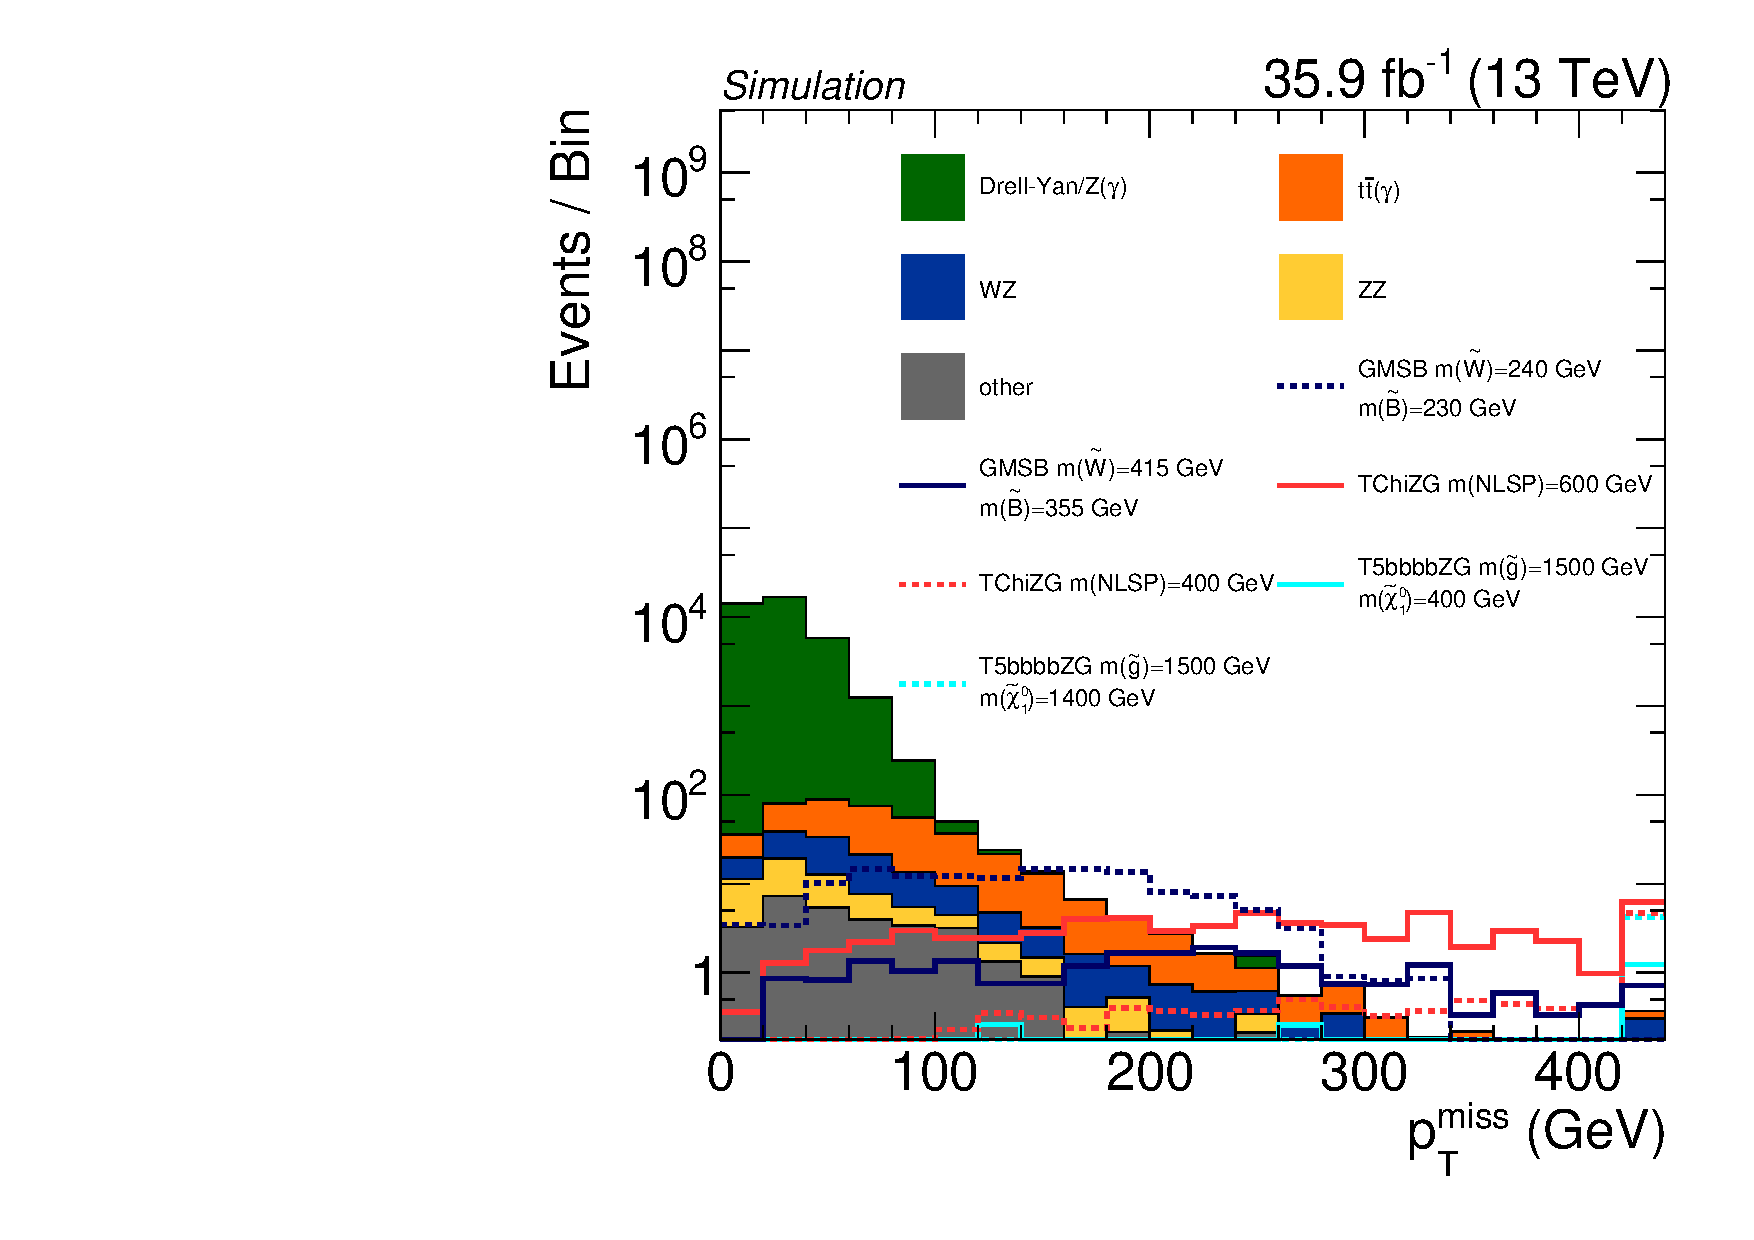
\includegraphics[width=\pairwidth]{figures/plots/onZ_LL_met_log}
 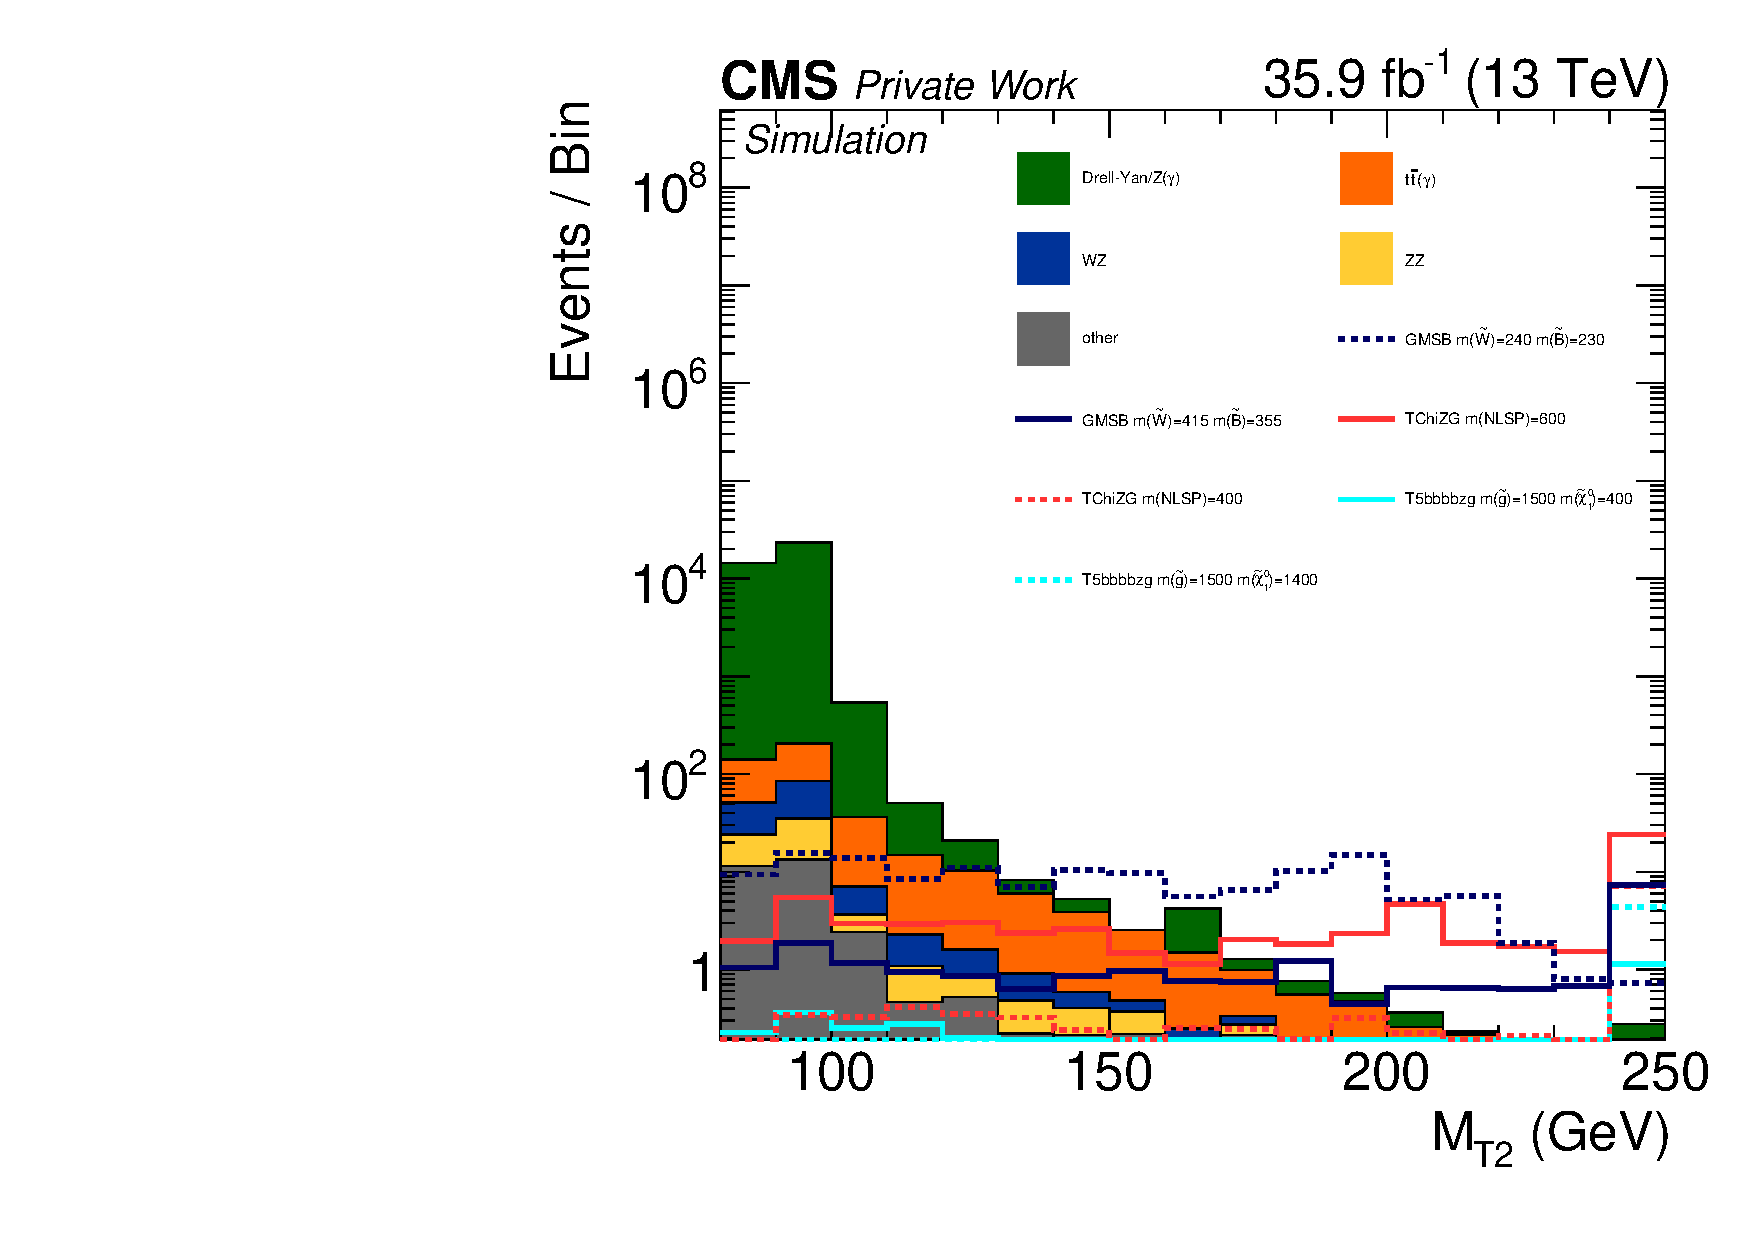
\includegraphics[width=\pairwidth]{figures/plots/onZ_LL_mt2_log}
 \caption{Stacked background events and events for different signal points against $\ptmiss$ (left) and $\mtTwo$ (right). Both are obtained from simulation. For each signal model two different signal points are shown. For their mass parameters refer to the legend in the plots.}
 \label{fig:SRvariables}
\end{figure}
The final SR is divided in two search bins in the $\ptmiss$ distribution, one ranging from $150$ to $200\GeV$, and the second one ranging from $200\GeV$ to infinity, see \refSec{sec:results}.

\subsection{Control regions}\label{sec:CR}
Different control regions (CRs) are defined for the four main background processes, in order to develop a background prediction for each background process. These CRs are built such that they are fully orthogonal to the signal region and among each other and include a large amount of events for precise studies and high purity. The main groups of backgrounds are $\ttbar(\PGg)$, DY/$\PZ(\PGg)$, $\PW\PZ$, and $\PZ\PZ$ production.

\subsubsection*{$\ttbar(\PGg)$ - control region}
To obtain a CR for the $\ttbar(\PGg)$ background, the flavor symmetry of the process is exploited. The two W bosons of the top quark decays can decay independently with the same probability to an electron or a muon, resulting in a similar number of same-flavor and different-flavor final state events. The different-flavor triggers are needed to guarantee a basis data set containing a sufficient number of events. In addition, the background can be studied in the same high $\ptmiss$ and $\mtTwo$ regions as the SR. The preselection criteria need to be adjusted accordingly, resulting in a CR definition of
\begin{itemize}
 \item exactly one different-flavor opposite-charge (DFOC) lepton pair ($\Pe\Pgm$),
 \item at least one photon,
 \item $\Delta R(\ell_1,\PGg)>0.3$ and $\Delta R(\ell_2,\PGg)>0.3$.
\end{itemize}
The invariant dilepton mass window requirement is removed from the preselection, since the reconstructed dilepton mass is not in coincidence with the Z boson mass. In contrast, it shows a broad distribution because the leptons are not originating from the same mother particle. The requirement being responsible for the orthogonality to the SR is the different dilepton flavor requirement.
\subsubsection*{Drell-Yan/$\PZ(\PGg)$ - control region}
The Drell-Yan/$\PZ(\PGg)$ background has nearly the same phenomenological topology as the SUSY signal, except for lower missing transverse momentum on average, since it mainly originates from mismeasurements of jets. The final control region definition additionally to the preselection is
\begin{itemize}
 \item $\ptmiss<100\GeV$.
\end{itemize}
This region is orthogonal to the SR due to the inverted $\ptmiss$ requirement.
\subsubsection*{$\PW\PZ$ - control region}
In order to obtain a high purity $\PW\PZ$ control region, the SFOC dilepton criteria are adjusted such that the fully leptonic decay of the diboson system is studied. As in the preselection, a SFOC lepton pair is required, but the additional lepton veto is inverted. Hence, the existence of a third lepton is required. Since the leptonic W boson decays are selected, with the help of additional $\ptmiss$ and $m_{T}$ requirements the purity of the selection of $\PW\PZ$ diboson production events is enhanced. The transverse mass $m_{T}$ is calculated using the third lepton and the missing transverse momentum, and is therefore an estimate for the $\PW$ boson mass. In the identification of the lepton pair belonging to the $\PZ$ boson, all combinations fulfilling flavor and charge requirements are tested. In case of multiple valid combinations, the combination with the invariant dilepton mass closest to the Z boson mass is chosen. To ensure a selection with a suitable amount of data, since the cross section for diboson production is rather low, the requirement of the existence of at least one photon from the preselection is removed. The final region selection is
\begin{itemize}
 \item exactly one SFOC lepton pair ($\Pe\Pe$ or $\PGm\PGm$),
 \item exactly one additional third lepton ($\Pe$ or $\Pgm$),
 \item $\Delta R(\ell_1,\PGg)>0.3$ and $\Delta R(\ell_2,\PGg)>0.3$,
 \item $81\GeV<m_{\ell\ell}<101\GeV$ (for the SFOC lepton pair),
 \item $\ptmiss>70\GeV$,
 \item $m_{T}(\ptvecmiss,\ptvec(\ell_3))>50\GeV$.
\end{itemize}
\subsubsection*{$\PZ\PZ$ - control region}\label{sec:VR}
The strategy to achieve a pure $\PZ\PZ$ diboson selection that does not overlap with the SR selection is very similar to the $\PW\PZ$ CR selection described above. By selecting events, where both $\PZ$ bosons decay leptonically to charged leptons ($\Pe\Pe$ or $\PGm\PGm$), per definition an exclusive control region is obtained. As in the $\PW\PZ$ CR selection, flavor and charge requirements are considered to construct $\Z$ boson candidates from the four selected leptons. In cases, where multiple valid solutions for the reconstruction of two $\PZ$ bosons exist, the possibility with the first Z boson candidate mass closest to the nominal Z boson mass is chosen. The second Z boson candidate has to fulfill a looser mass agreement compared to the first one. Also, the existence of a photon in the event is not required. In total, the selection criteria are
\begin{itemize}
 \item exactly two SFOC lepton pairs ($\Pe\Pe$ or $\PGm\PGm$),
 \item $\Delta R(\ell_1,\PGg)>0.3$ and $\Delta R(\ell_2,\PGg)>0.3$ for the first pair,
 \item $76\GeV<m_{\ell\ell}<106\GeV$ for the mass of the first Z boson candidate,
 \item $50\GeV<m_{\ell\ell}<130\GeV$ for the mass of the second Z boson candidate.
\end{itemize}
\subsubsection{Validation region}
An additional validation region (VR) is constructed, where the developed background predictions are verified by performing data-to-background prediction comparisons. Therefore, it is convenient to choose a VR close in phase space to the SR. This is achieved by applying the same selection requirements as for the SR, but demanding either the $\ptmiss$ or the $\mtTwo$ requirement to be inverted. The VR must also not overlap with the DY/$\PZ(\PGg)$ CR, thus a minimal $\ptmiss$ requirement needs to be imposed. The selection requirements for the VR in addition to the preselection are the following:
\begin{itemize}
 \item $\ptmiss>100\GeV$,
 \item either $\ptmiss<150\GeV$ or $\mtTwo>100\GeV$.
\end{itemize}
A visualization of the signal, validation, and DY/$\PZ(\PGg)$ control region definitions in the $\mtTwo$ - $\ptmiss$ plane can be found in \refFig{fig:Regions}. Two dimensional histograms for the number of expected events motivating the region definitions are shown in \refFig{fig:Regions2} for all background processes, together with distributions of different benchmark signal points for all three considered signal models.
\begin{figure}[tbp]
 \centering
 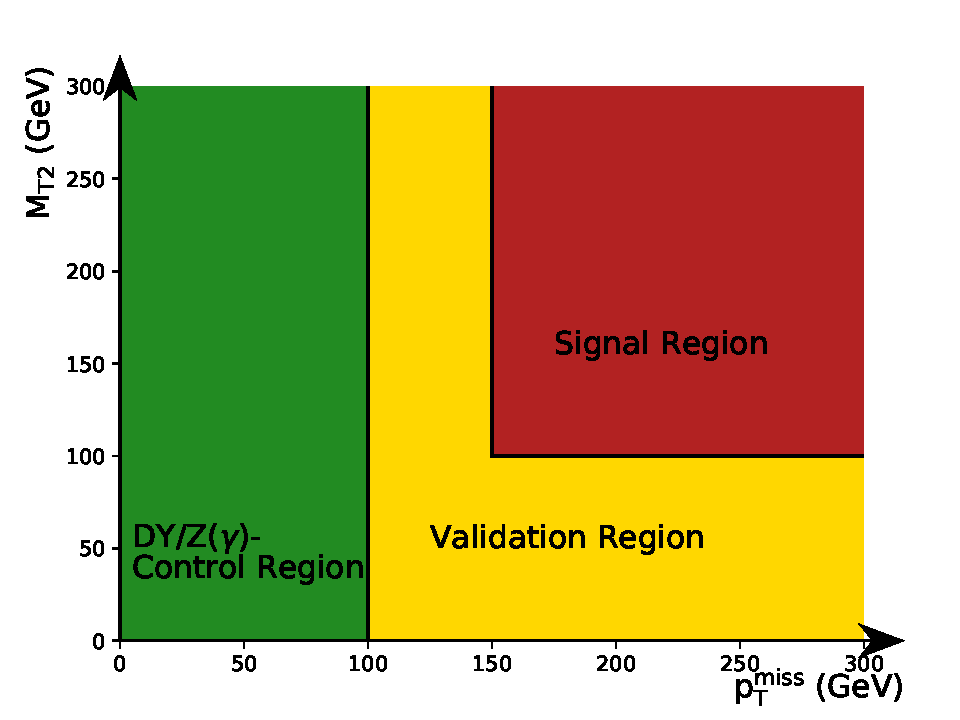
\includegraphics[width=\pairwidth]{figures/figures/regions}
 \caption{Visualization of the definition of the signal, validation, and DY/$\PZ(\PGg)$ control region in the $\mtTwo$ - $\ptmiss$ plane.}
 \label{fig:Regions}
\end{figure}
These distributions show also specific features of the considered signal models regarding important kinematic observables. Because the \texttt{TChiZG} model is a one parameter scan, and the only free parameter is the NLSP mass, together with the momentum of the NLSP it directly determines the maximum amount of transverse momentum for the decay products and thus directly the Z boson $\pt$ and the $\ptmiss$ originating from the gravitinos. Also, the endpoint of the $\mtTwo$ distribution is of the same order and coincide with the NLSP mass. Hence, $\ptmiss$ and $\mtTwo$ calculated from the bosons and $\ptmiss$ are strongly correlated.\\
In case of the strong SMS, it is not directly the case. Since this is a two dimensional parameter scan, the event kinematics also depend on the mass difference of the gluino and the NLSP mass, as discussed in \refSec{sec:SMS}. In cases where the mass difference is small, the kinematics evolve similar as for the EWK SMS, while for larger mass differences, as shown in \refFig{fig:Regions2}, the correlation between $\mtTwo$ and $\ptmiss$ is much weaker and the distributions are much broader. The distributions of the GMSB model behave similar to the electroweak SMS, depending on the wino and bino masses.\\
The signal events mainly populate the SR for all models, with small contributions in the CRs and the VR, while the majority of the background events contribute to the DY/$\PZ(\PGg)$ CR and a minor part to the VR. Only a minority of the background events are expected in the SR. Hence, in total a good separation between background and signal is achieved.

\begin{figure}[tbp]
 \centering
 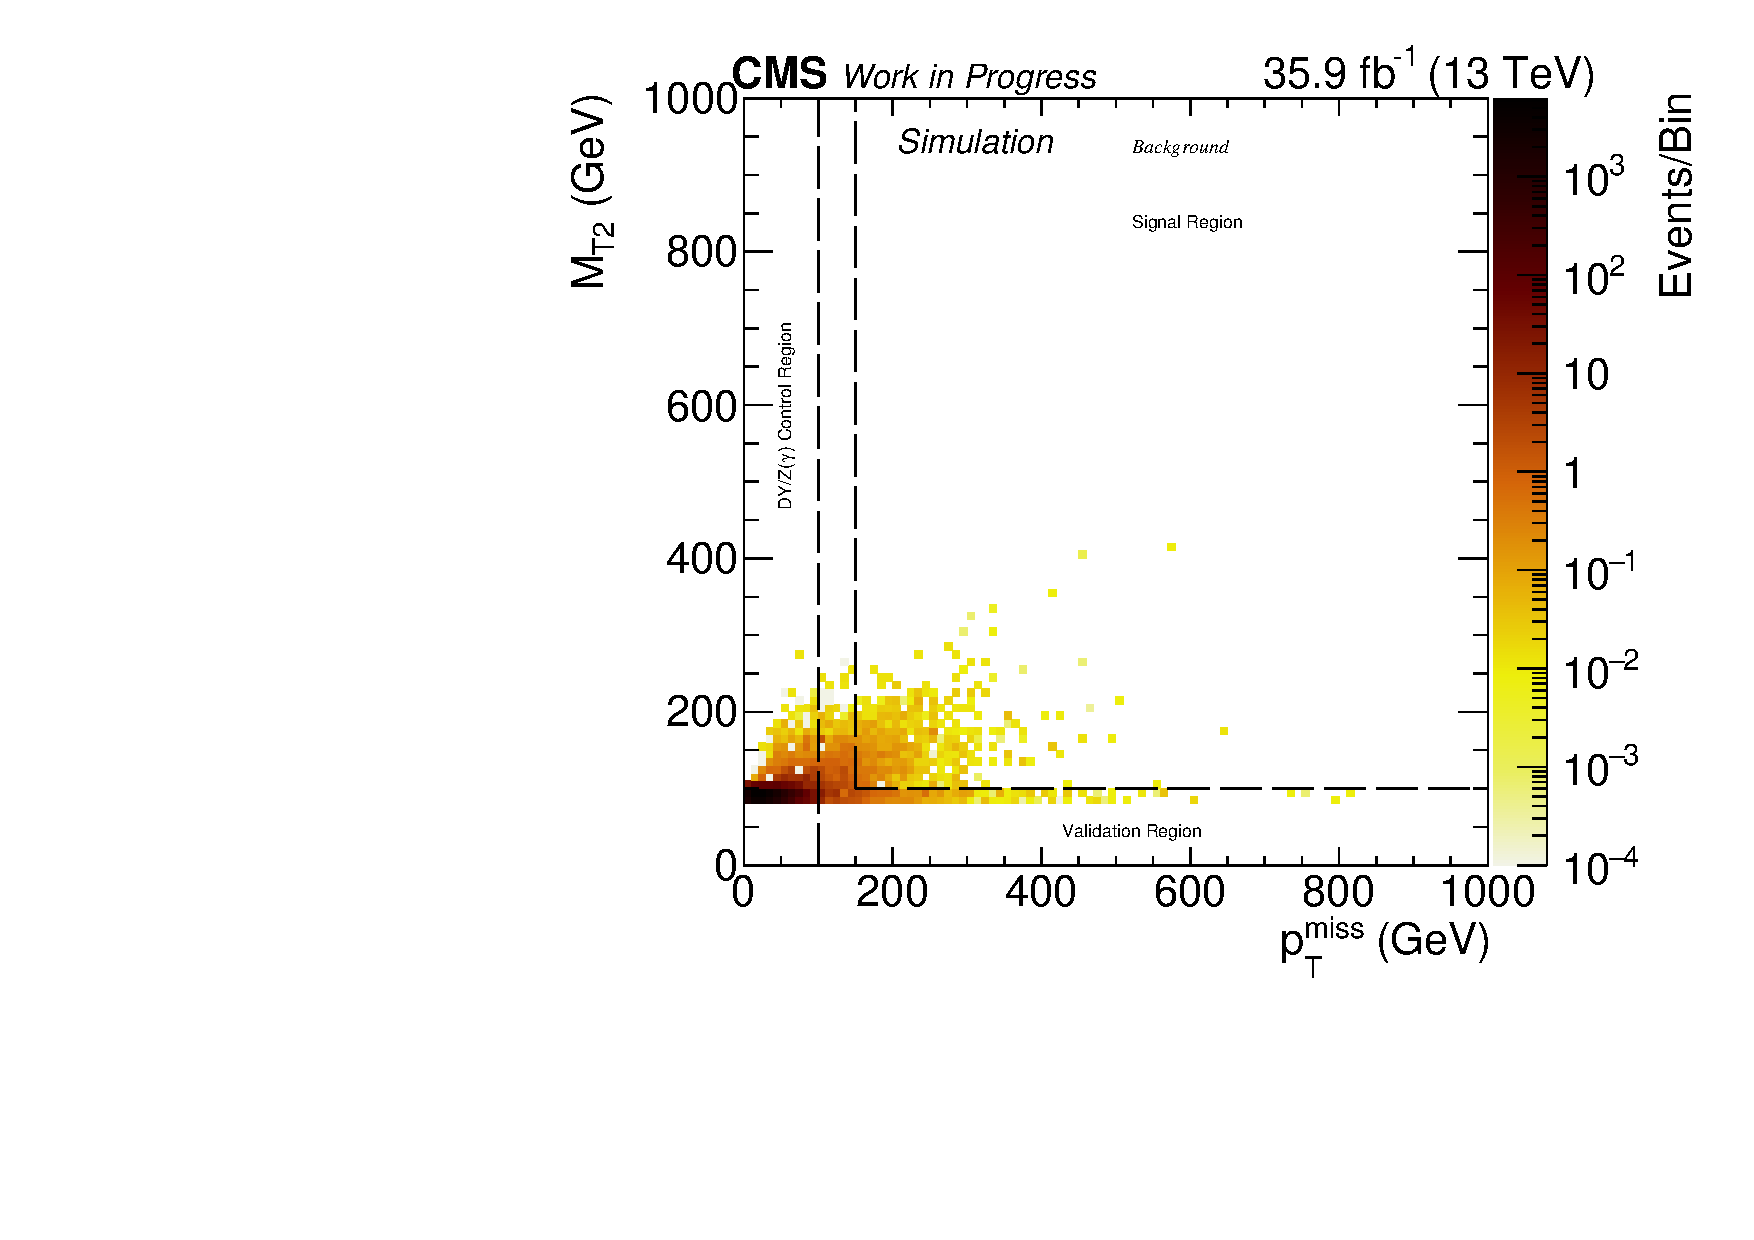
\includegraphics[width=\pairwidth]{figures/plots_2d/DataMC_sameHistograms_LL+signal_onZ__LL__MetMt2_bkg_}
 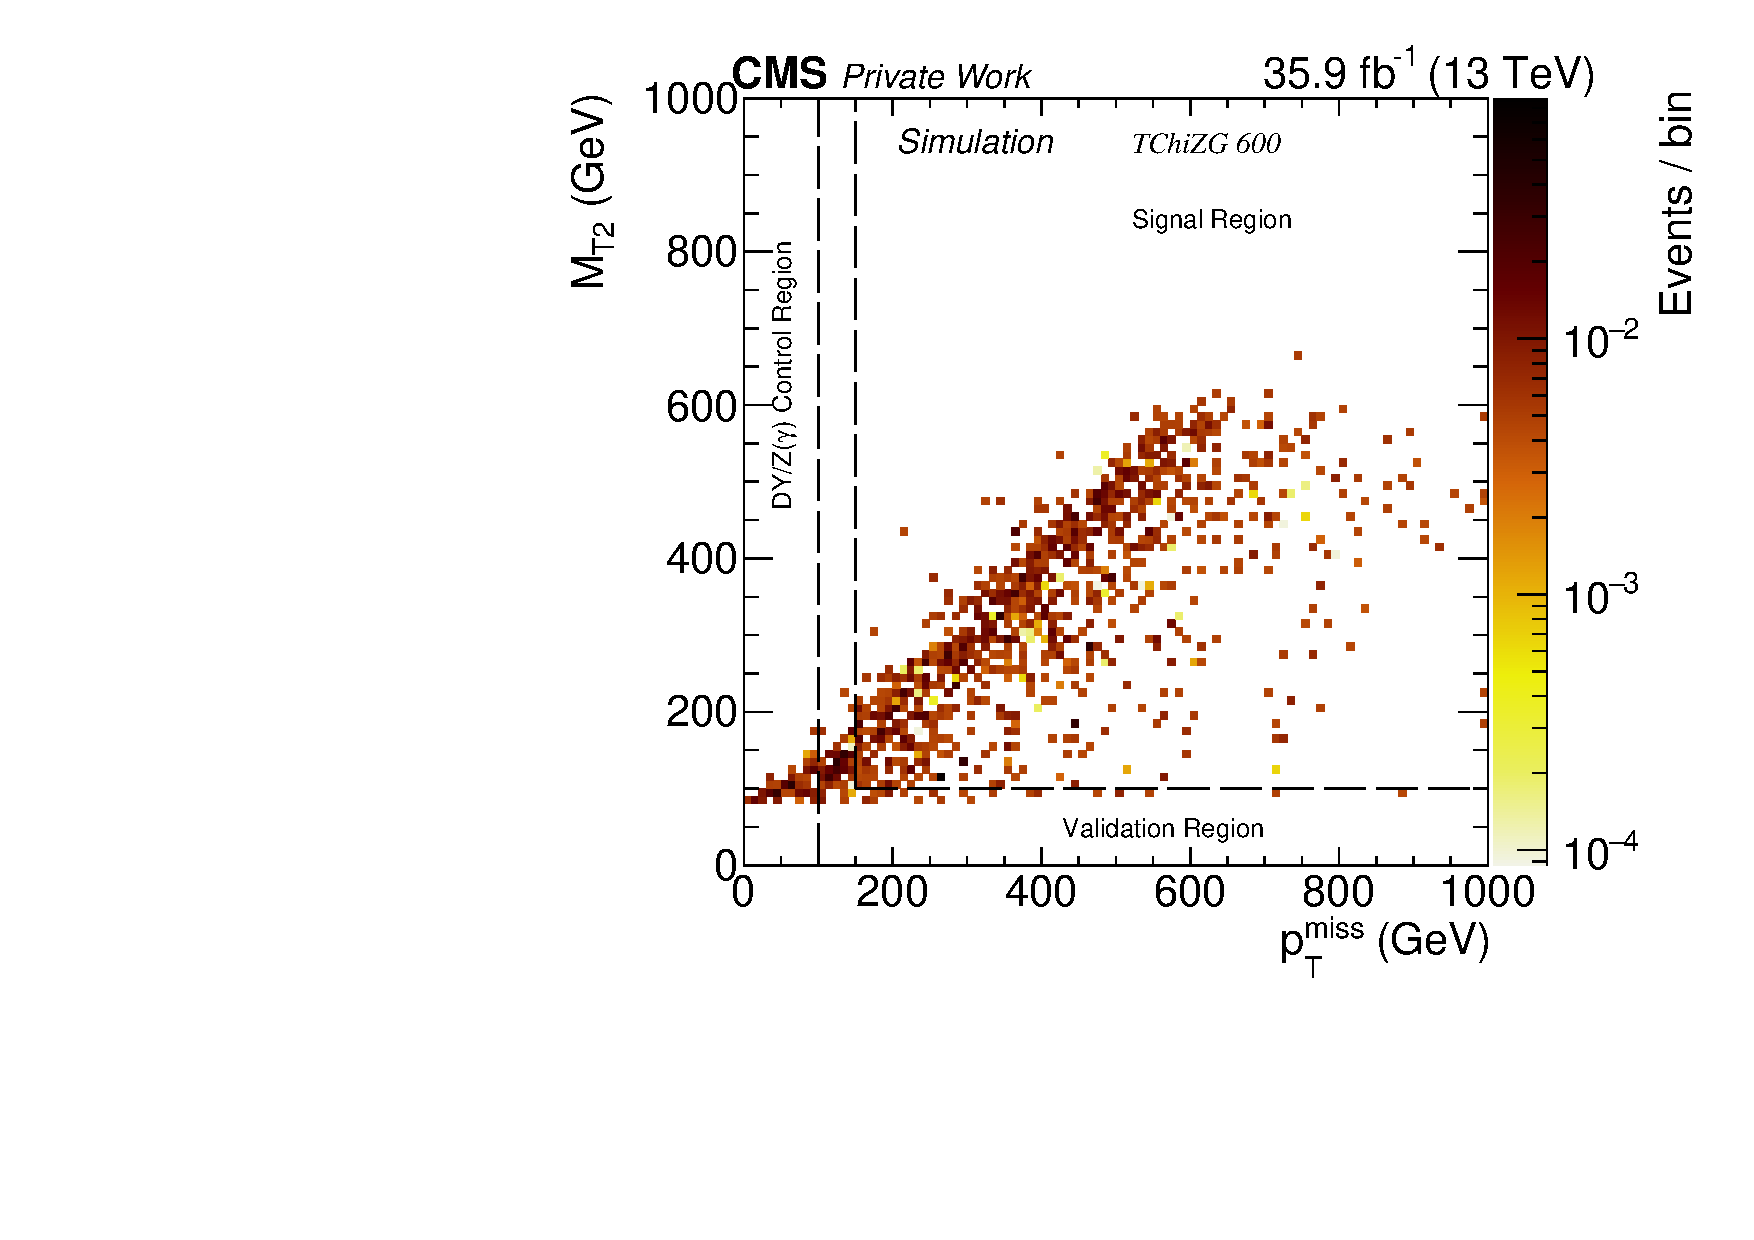
\includegraphics[width=\pairwidth]{figures/plots_2d/DataMC_sameHistograms_LL+signal_onZ__LL__MetMt2_SIG_tching600_}\\
 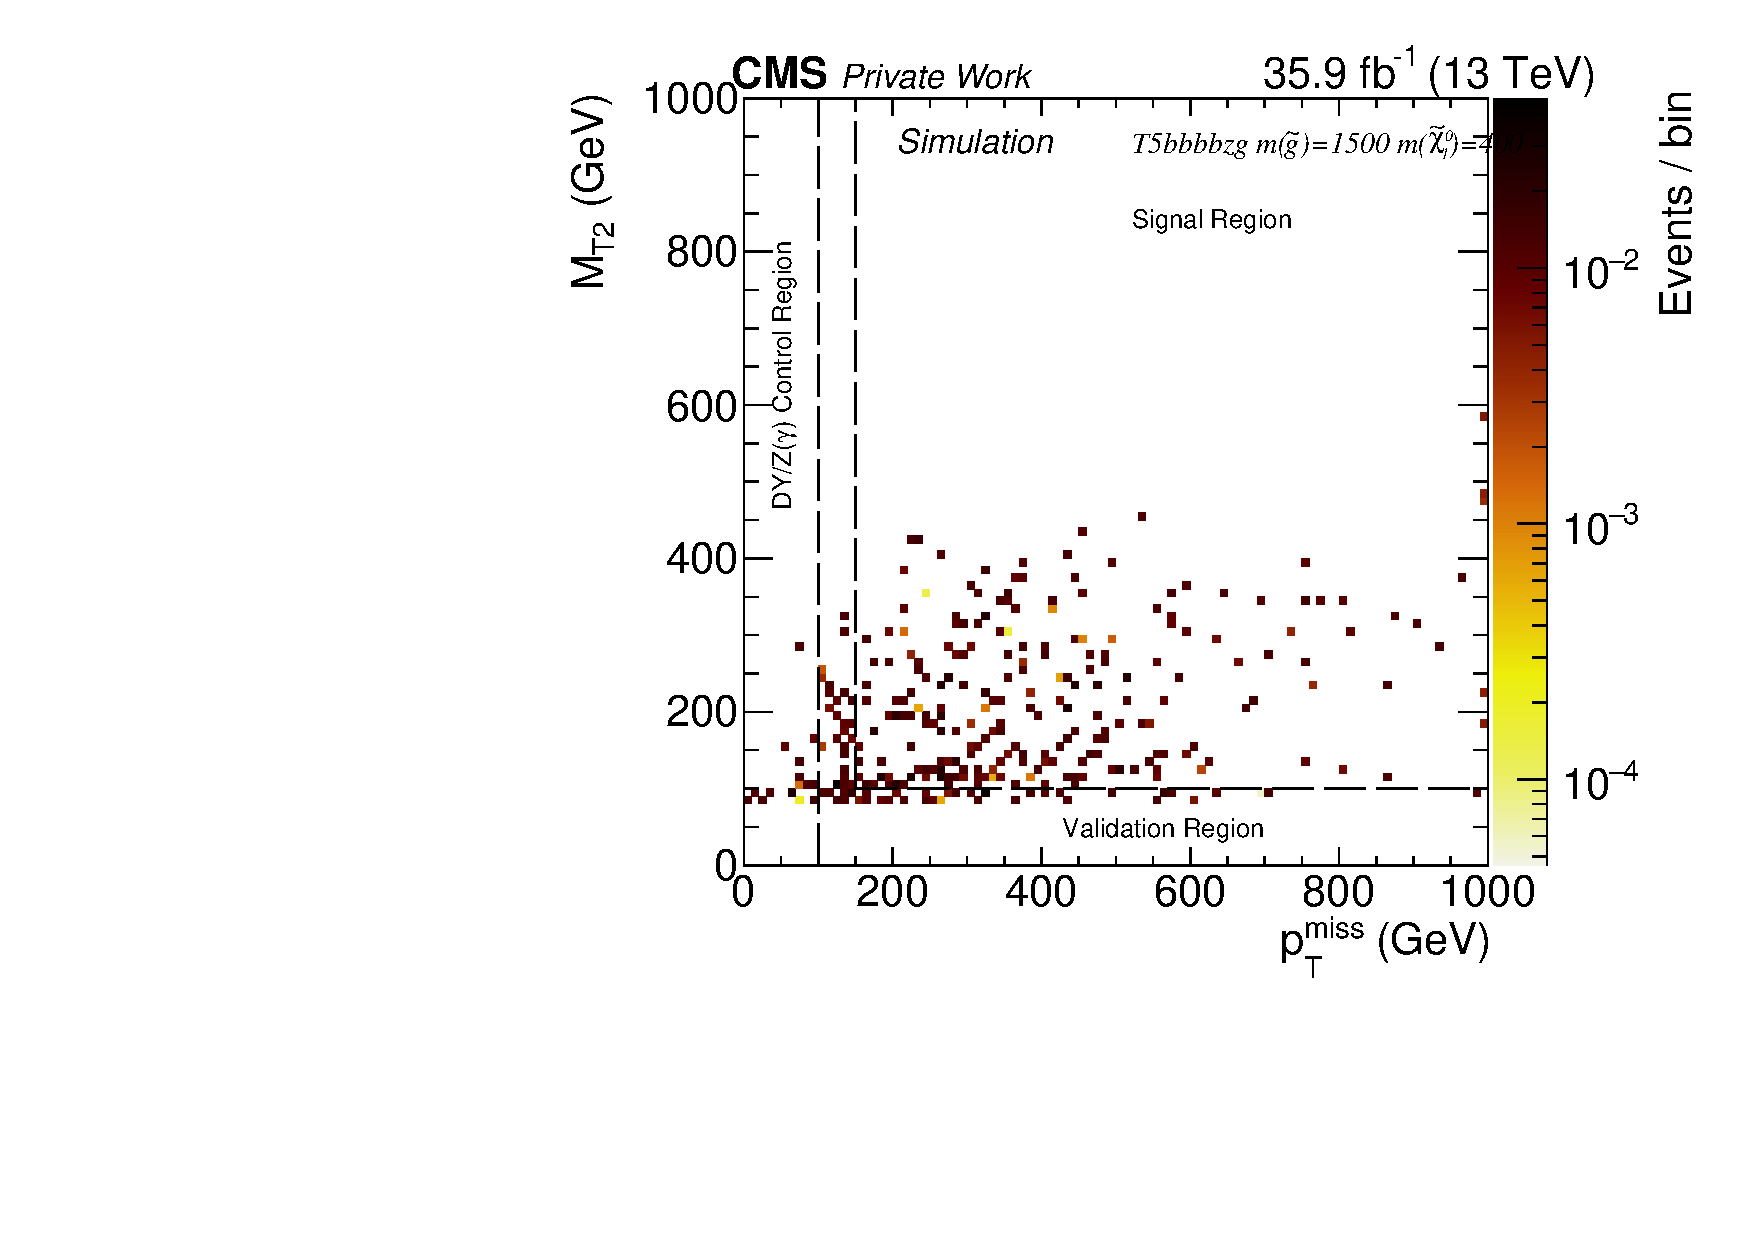
\includegraphics[width=\pairwidth]{figures/plots_2d/DataMC_sameHistograms_LL+signal_onZ__LL__MetMt2_SIG_t5bbbbzg_1500_400_}
 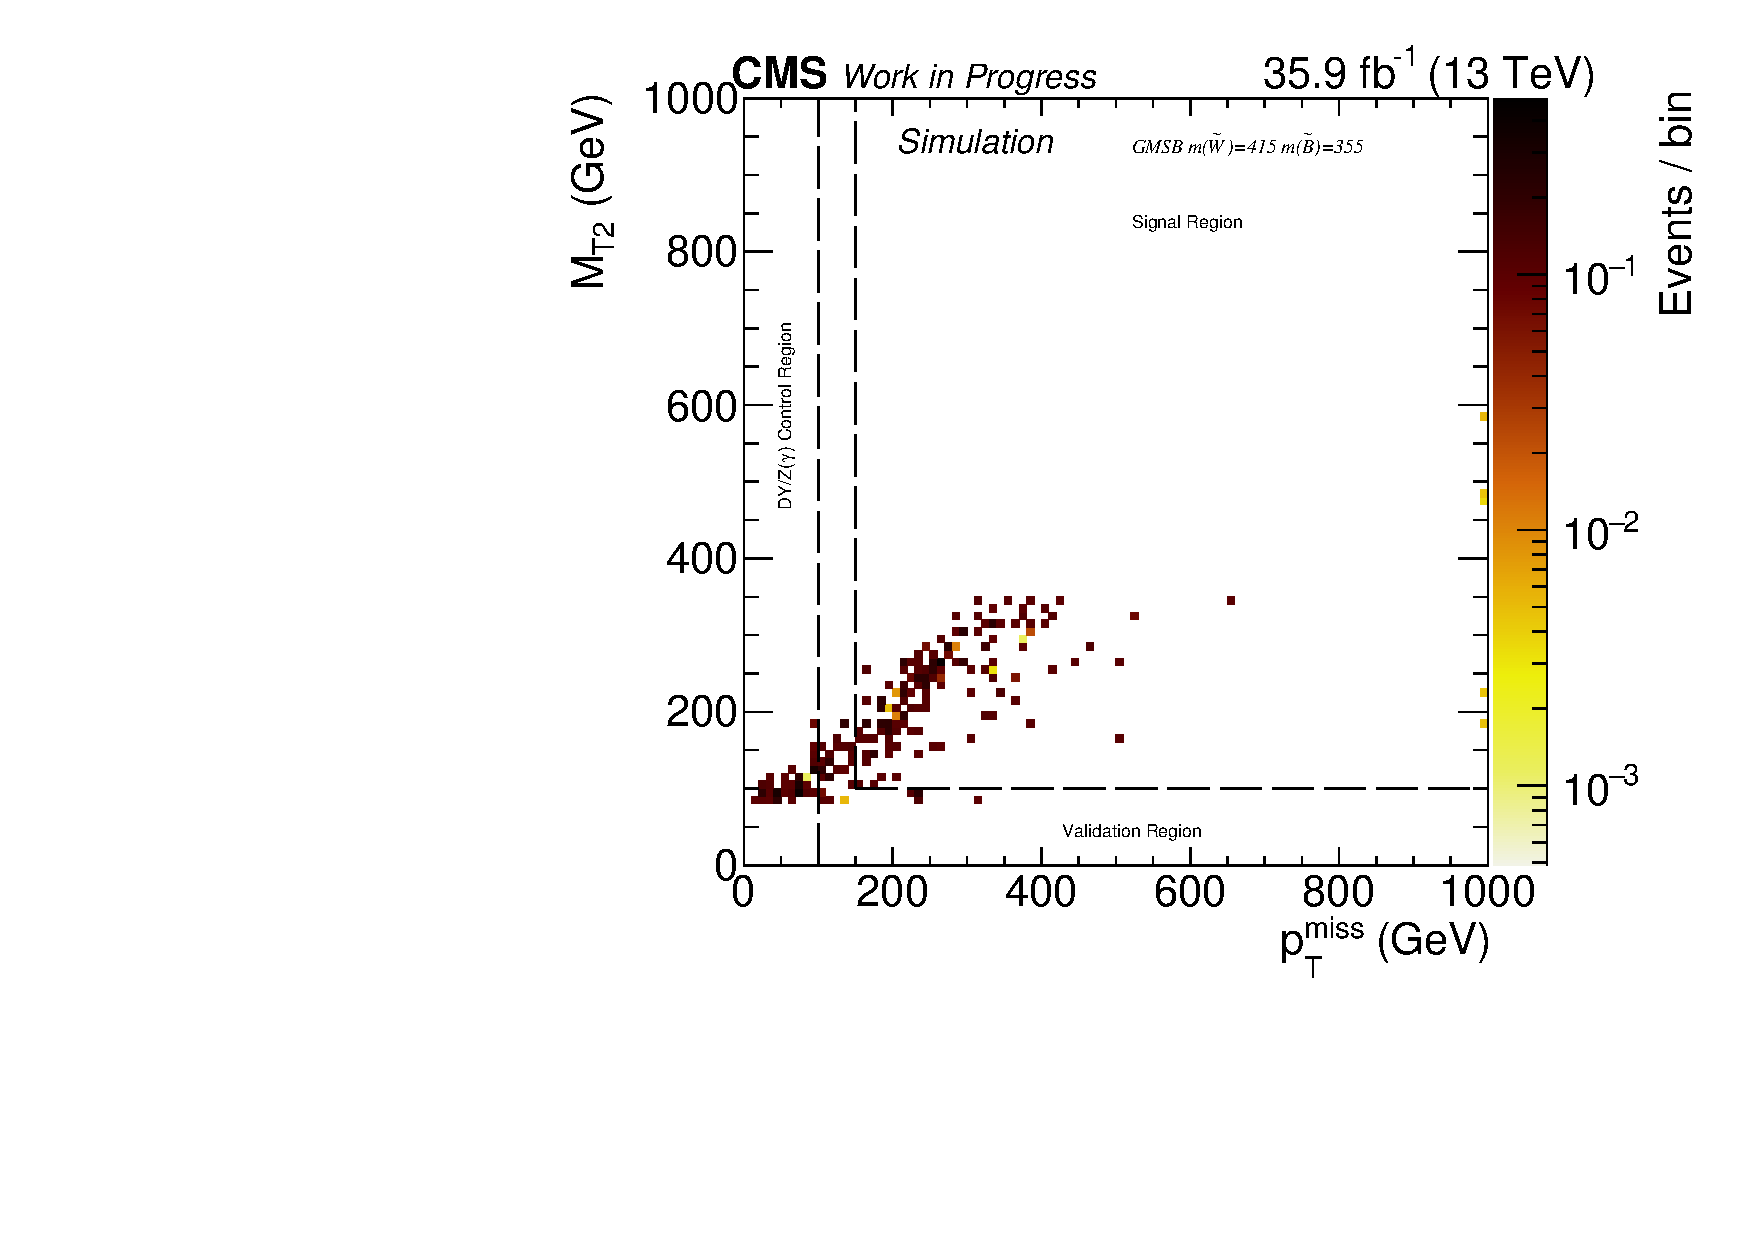
\includegraphics[width=\pairwidth]{figures/plots_2d/DataMC_sameHistograms_LL+signal_onZ__LL__MetMt2_SIG_gmsb_415_355_}
 \caption{Distribution of the total number of expected background events in the $\mtTwo$ - $\ptmiss$ plane (upper left). Distributions for the number of expected signal events for the \texttt{TChiZG} SMS with an NLSP mass of $600\GeV$ (upper right), the \texttt{T5bbbbZG} SMS with a gluino mass of $1.5\TeV$ and a neutralino mass of $400\GeV$ (bottom left), and the GMSB model with $m(\widetilde{W})=455\GeV$ and $m(\widetilde{B})=355\GeV$ (bottom right).}
 \label{fig:Regions2}
\end{figure}



\section{Background estimation}\label{sec:BKG}
In this section, the used background estimation methods are discussed, including the study of systematic effects. The total background is composed of $\ttbar(\PGg)$ production, Drell-Yan and $\PZ(\PGg)$ events, $\PW\PZ$ and $\PZ\PZ$ diboson production, and a remaining group of backgrounds ("other"), composed of, \eg, single top and triboson production (See \refSec{sec:Simulation} and \refSec{sec:CR}). The relative contributions for all background processes in the two SR bins are depicted in \refFig{fig:PieCharts}. The most dominant background is $\ttbar(\PGg)$, followed by $\PW\PZ$, $\PZ\PZ$, and Drell-Yan/$\PZ(\PGg)$.\\
The leptonic decays of the top pairs generated in association with a photon significantly contribute to the SR, because the final state signatures appear very similar to those of the SUSY models and the production cross section is very high. If both $\PW$ bosons decay leptonically, a SFOC lepton pair in connection with neutrinos can be produced, creating a large amount of $\ptmiss$ in the detector. Prompt photons can be produced in the hard interaction, or can be radiated off in the initial or the final state by participating charged particles. Since the two selected leptons of the $\ttbar$ system decay originate from different mother particles, the reconstructed invariant mass distribution shows is broad and shows no resonance. Due to the high cross section of the $\ttbar(\PGg)$ production, see \refTab{tab:MCsamples}, there is a sufficient probability to measure an invariant dilepton mass close to the Z boson mass although the two leptons do not emerge from it.\\
In the Drell-Yan process and in $\PZ\PGg$ production, an on-shell Z boson is produced, thus the $\m_{\ell\ell}$ requirement for the dileptons in the SR is fulfilled. Although a photon can be produced additionally, this background does not contribute significantly to the SR, because only nongenuine $\ptmiss$ is generated in the process due to mismeasurements and therefore the $\ptmiss$ distribution is steeply falling.\\
$\PW\PZ$ production is also an important background for this search, since the $\PW$ boson can decay leptonically and therefore creates a sufficient amount of genuine $\ptmiss$ to pass the SR requirements, but is also suppressed by the $\mtTwo$ requirement. While a photon can be generated in all possible radiation processes, an additional electron or jet originating from the $\PW$ boson can fake a photon signature in the detector. In cases of appearance of photons, events can contribute, where the additional lepton does not pass the acceptance, reconstruction, and identification criteria.\\
Lastly, the $\PZ\PZ$ event signature can be very similar to the one expected from the considered SUSY signals. One boson can decay to a pair of charged leptons, while the other decays to neutrinos leading to a large amount of $\ptmiss$ in the event. Together with FSR or ISR of a photon, $\PZ\PZ$ background events show a signature very similar to the signal topology.\\
If the different background processes are compared, the diboson processes have more similar event kinematics than the $\ttbar(\PGg)$ process compared to the signal processes, but due to the lower diboson production cross sections the $\ttbar(\PGg)$ background dominates the other contributions.
\begin{figure}[tbp]
 \centering
 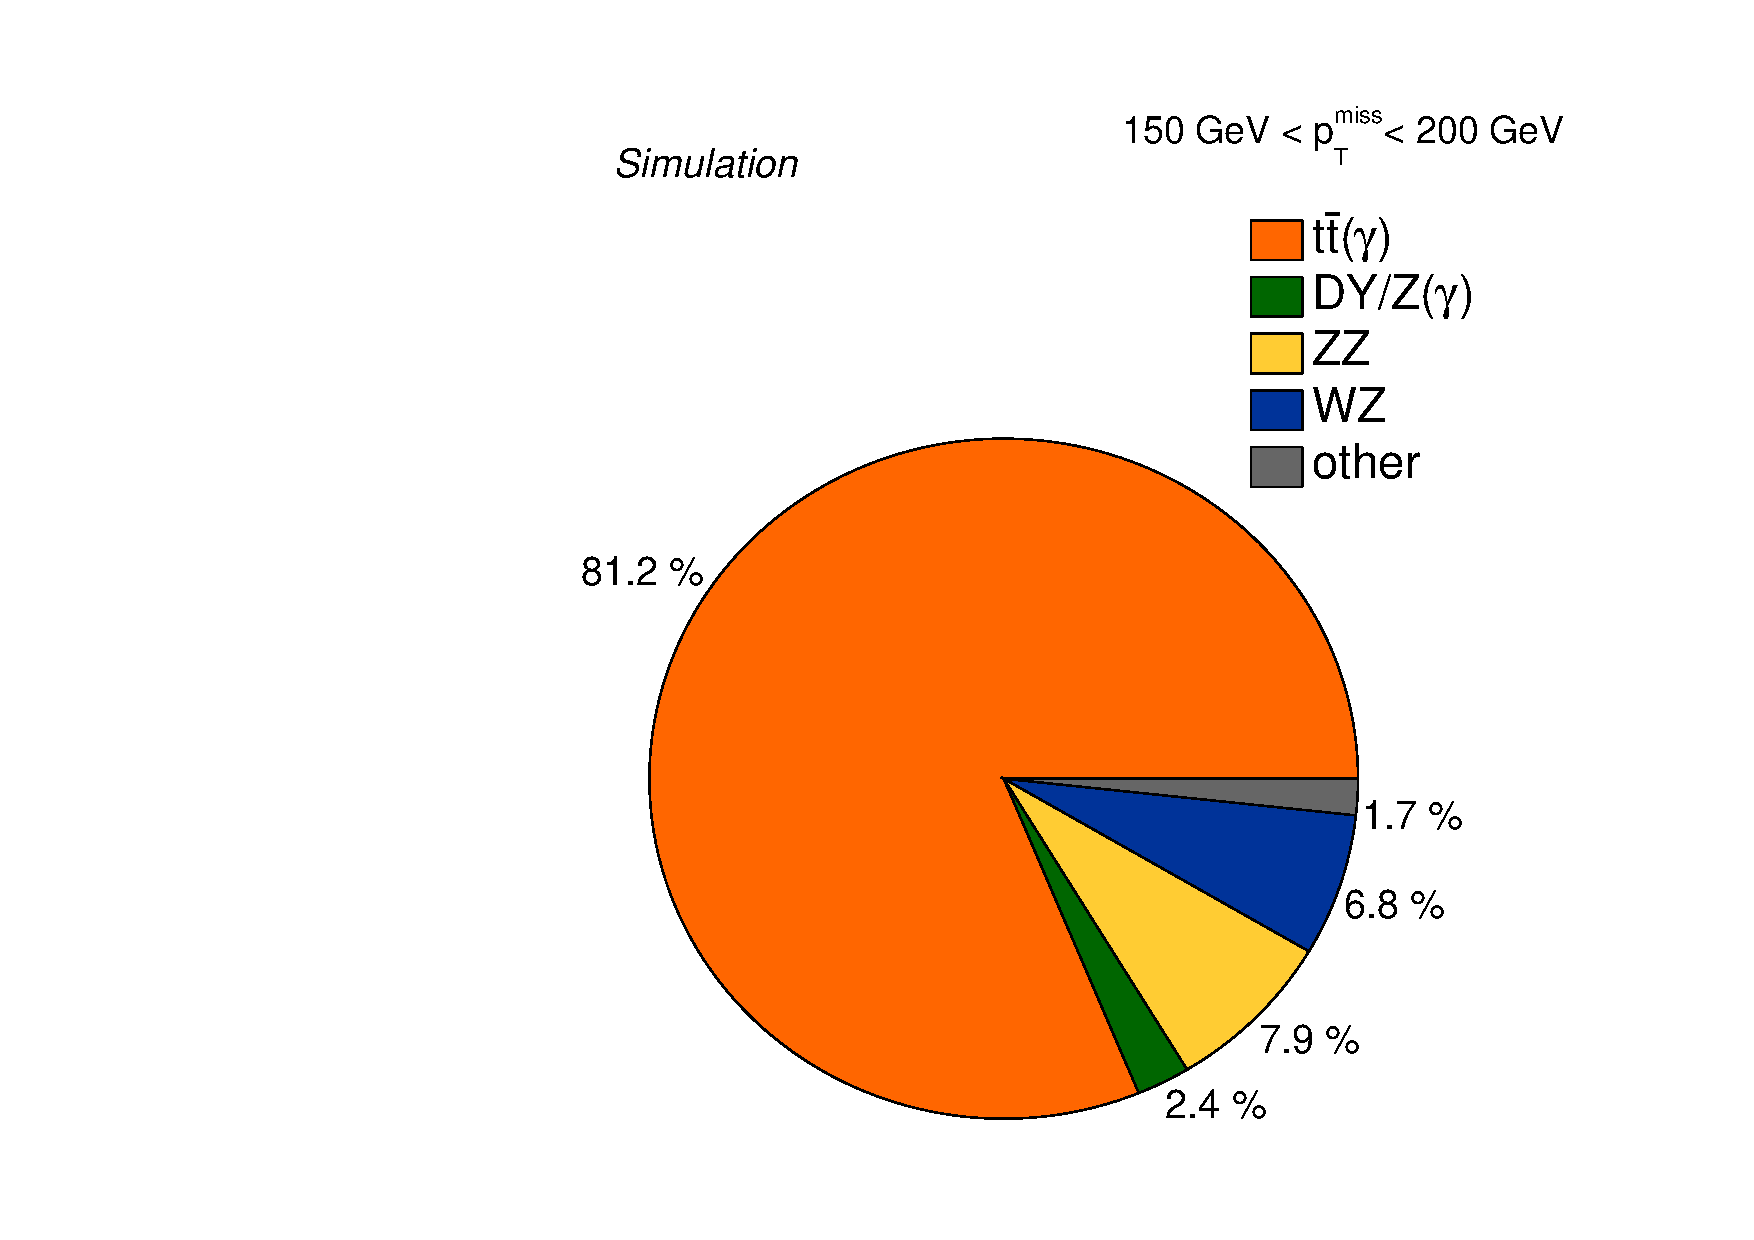
\includegraphics[width=\pairwidth]{figures/figures/pie1}
 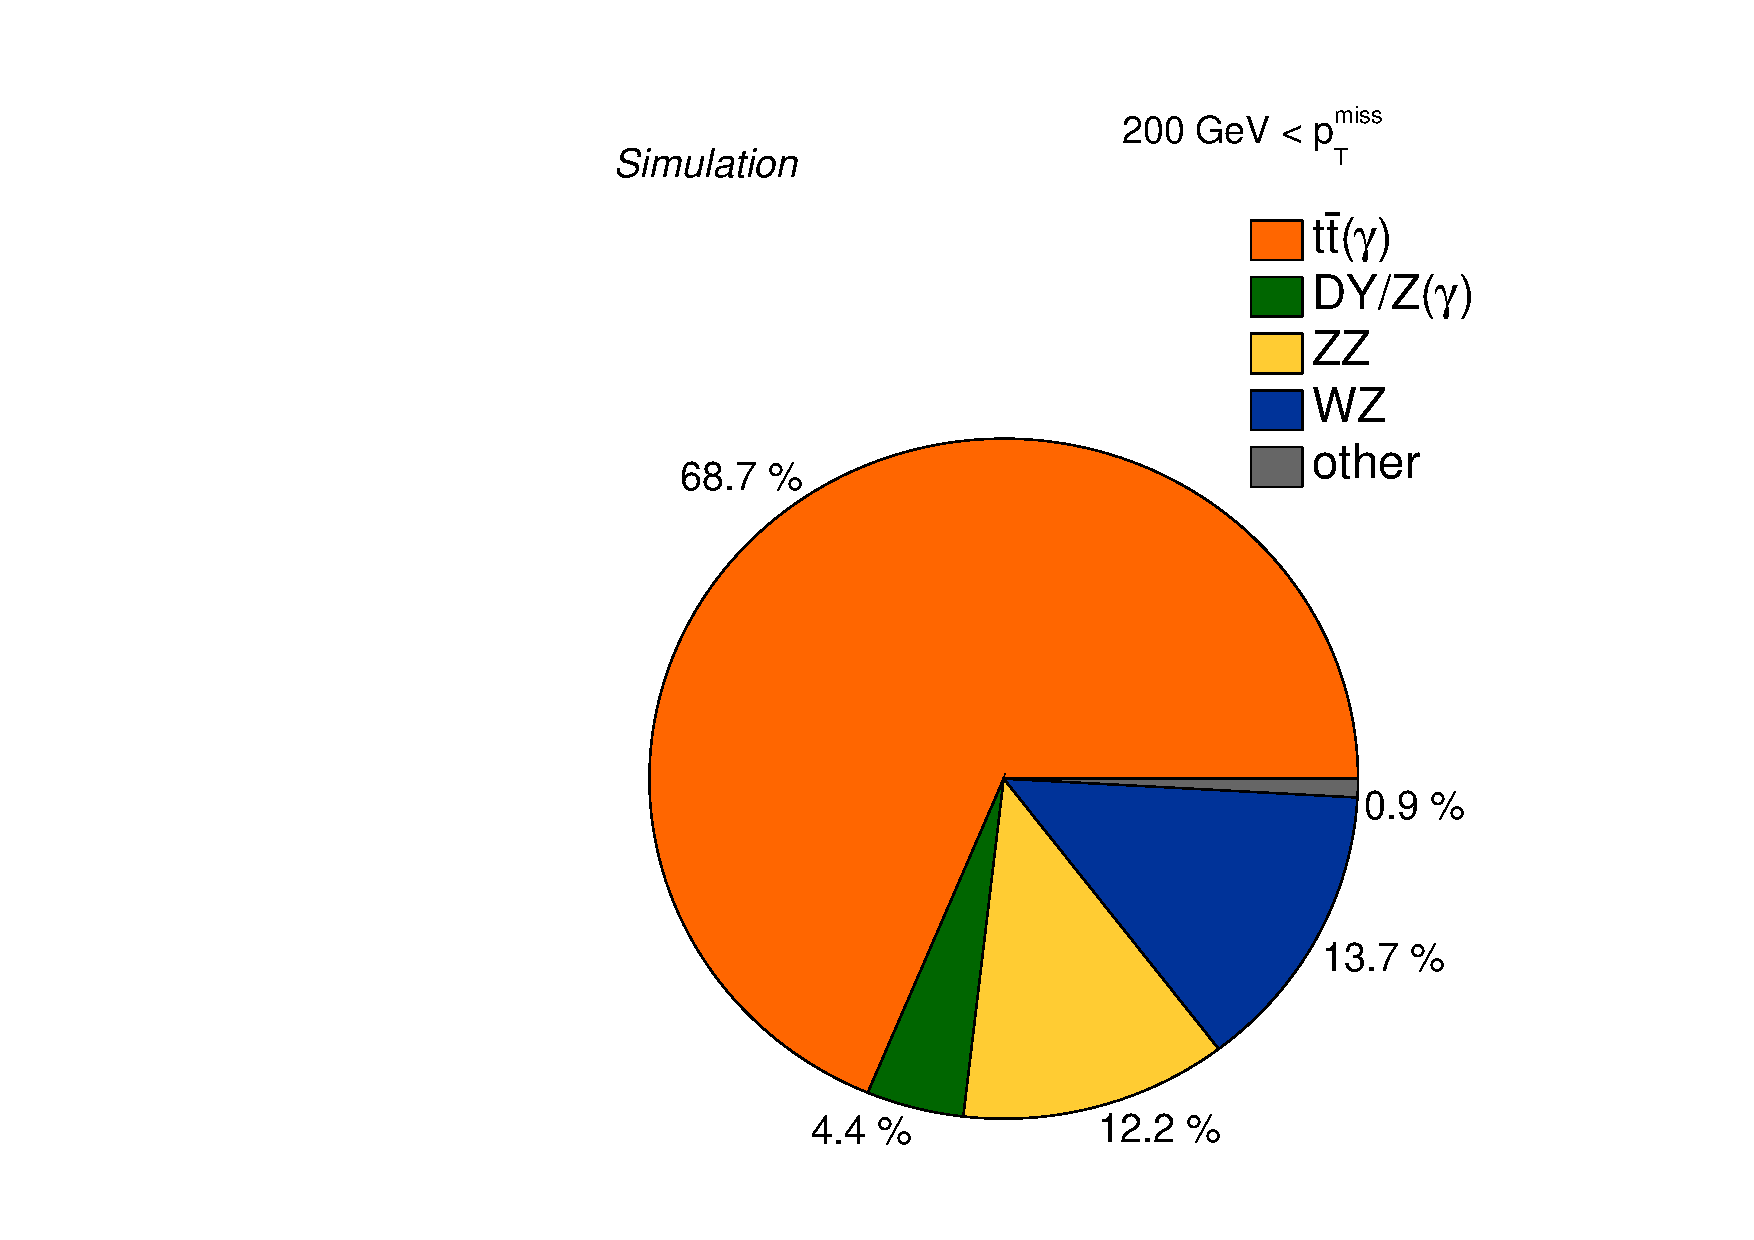
\includegraphics[width=\pairwidth]{figures/figures/pie2}
 \caption{Relative amounts for all groups of considered backgrounds for the two search bins in the SR.}
 \label{fig:PieCharts}
\end{figure}
The background prediction is based on simulation for all backgrounds. As mentioned in \refSec{sec:CR}, different CRs are developed, that are enriched with corresponding background events. In those CRs, scale factors (SF) $\alpha_i$ are calculated by scaling the simulation to the measured data yield. Contributions of other backgrounds in the CR are considered in the calculation by fixing their contribution. The SFs are calculated via the following formula:
\begin{align}
 1                        & = \frac{D}{F+\alpha_i\cdot B} \\
 \Longrightarrow \alpha_i & = \frac{D-F}{B},              
\end{align}
where $B$ is the number of background events that are to be scaled, $F$ the number of fixed background events, and $D$ the number of measured data events.
Due to the used method, which is performed similarly in each CR, possible uncertainties on the normalization of the predicted distributions cancel, and only uncertainties in the shape need to be considered, see~\refSec{sec:Syst}. The uncertainty arising from the SF calculation is purely of statistical origin, and is calculated via error propagation
\begin{equation}
 \sigma_{\alpha_i}^2 = \sigma_{D}^2 \cdot \left(\frac{D}{B}\right)^2 + \sigma_{F}^2 \cdot \left(\frac{F}{B}\right)^2 + \sigma_{B}^2 \cdot \left(\frac{D-F}{B^2}\right)^2,
\end{equation}
where $\sigma_i$ are the corresponding statistical uncertainties to $D$, $F$, and $B$. These are assumed to be uncorrelated Poissonian uncertainties, and can be calculated via $\sigma_i=\sqrt{N_i}$, where $N$ is the associated integral of events in the selection. In the case of simulation, for the calculation of the SF the normalized event yield is used, whereas in the error calculation the pure MC event count is considered to reflect the underlying statistical precision of the simulation. This method is referred to as the "integral method" in the following.\\
In each CR, all other background contributions have an influence, since their contributions are not negligible. Therefore, the order of SF determination can introduce a bias. To minimize this effect, the SFs are calculated in descending order of the purity of the background sample. At first, the $\PZ\PZ$ SF is determined, followed by DY/$\PZ(\PGg)$, $\ttbar(\PGg)$, and $\PW\PZ$. However, the background estimations are discussed in a different order, starting with the most important background, $\ttbar(\PGg)$. The systematic uncertainty arising from the choice of order is discussed in \refSec{sec:Syst}.\\
To strengthen the confidence in the outcome, Kolmogorov-Smirnov (KS)~\cite{KS} tests are performed to study the agreement of measured and predicted shape, which are based on the largest deviation between the two compared distributions. Resulting KS-values from the tests results are quoted on the corresponding plots for each individual distribution in the related sections. KS-values $\ll1$ indicate disagreement between the input distributions, otherwise the distributions are considered to match.\\\\
In order to study a possible bias of observables not well modeled within the simulation, additional cross checks are performed. Similar to the SF calculation in the integral method, SFs are determined via $\chi^2$-minimization in the same CRs. Albeit this method is somewhat correlated to the method explained above, it enables the possibility to study influences of different distributions in different binnings. Therefore, for the final SF determination the integral method is preferred over the $\chi^2$-method, since it is independent of the choice of any observable or binning and the resulting values for $\alpha_i$ agree between both methods. Thus, the $\chi^2$-fits serve only as additional cross-checks. In order to obtain the SF via $\chi^2$-minimization, the $\alpha_{i}$ is varied in a range in small steps for each binning and distribution, and for every iteration the simulation is scaled and the $\chi^2$ is calculated, which is defined as:
\begin{equation}
 \chi^2=\sum_i^{N_{bins}} \frac{\left(N_{i}^{obs}-N_{i}^{pred}\right)^2}{N_{i}^{pred}}.
\end{equation}
The best fit value is determined to be at the minimum of the $\chi^2$-distribution, which is obtained by fitting a polynomial of fourth grade to the $\chi^2$-distribution. Ideally the measured $\chi^2$-distribution would be described by a parobola, but in order to account for asymmetries in the determined distribution, a higher order polynomial is chosen as the fit function. In addition, the fits do not have a statistical influence, but are only needed to extract the best fit value and its uncertainty, which is also of statistical origin. It is calculated by taking the difference between the best fit value and the values, corresponding to $\chi^2=\chi^2_{BestFit}+1$. An example fit in the $\ptmiss$ distribution is shown in \refSec{sec:ttbar} in the discussion of the $\ttbar(\PGg)$ background estimation. The number of degrees of freedom ($ndf$) is given by the number of bins used to obtain the $\chi^2$-distribution reduced by the number of parameters that are being optimized. The only free parameter is $\alpha_{i}$, so $ndf$ equals the number of bins subtracted by unity.\\
After determining all SFs, the background prediction is tested in the VR. Therefore, the simulated backgrounds in the VR are scaled accordingly, and the result is investigated, see \refSec{sec:Validation}.



\subsection{Top pair production}\label{sec:ttbar}
As shown in \refFig{fig:PieCharts}, the main background contribution is $\ttbar(\PGg)$, which is composed of standard top pair production with and without photon radiation, and top-pair production in association with a photon, while the latter dominates. Both compositions are determined together by rescaling the simulation, such that the integral of events of the simulation in the CR matches the integral of events in data as explained in \refSec{sec:BKG}. The overall purity of the selection is of the order of $85\%$.
% For the scaled event yields, only weights to account for the trigger efficiency correction and a global weight as mentioned in \refSec{sec:Simulation} to normalize the simulation to the physical expectation are made use of.
% \begin{table}[tbp]
%  \centering
%  \caption{Yields in the $\ttbar(\PGg)$ CR for the pure simulation and measured data.}
%  \label{tab:CRTT}
%  \begin{tabular}{llll}
%
%   process      & raw simulation & simulation & data                  \\\hline
%   $\ttbar$     & 12077          & 416.93     &                       \\
%   $\ttbar\PGg$ & 128396         & 1420.19    &                       \\\hline\hline
%   sum          & 140473         & 1837.12    & \multirow{2}{*}{1750} \\
%   other        & 14631          & 275.25     &
%  \end{tabular}
% \end{table}
With the integral method applied, the SF is obtained and given by
\begin{equation}\label{eq:AlphaTT}
 \alpha_{\ttbar(\PGg)}=0.80 \pm 0.03 (stat.) [\hat{=}4.0\%].
\end{equation}
After application of $\alpha_{\ttbar(\PGg)}$, the numbers of events in data and simulation match per definition.\\
Since the analyzed final state in this CR is very sensitive to higher order effects such as jet and photon radiation, and complex matrix elements are needed to describe the hard interaction, a SF differing from unity meets the expectation. NNLO electroweak effects can cause negative corrections for example due to destructive terms in higher order corrections.
The uncertainty of the order of $4\%$ indicates, that a sufficient number of events is present in the corresponding CR.\\
The resulting prediction shows a good agreement with data, as can be seen from the $\ptmiss$ and $\mtTwo$ distributions in the CR after rescaling in \refFig{fig:CRTT}. The uncertainty of the fit method is of statistical origin, and is treated as a systematic uncertainty in the following. The agreement of additional important observables, such as the transverse momentum of the photon and both leptons, is also investigated, and no systematic deviation was found.
\begin{figure}[tbp]
 \centering
 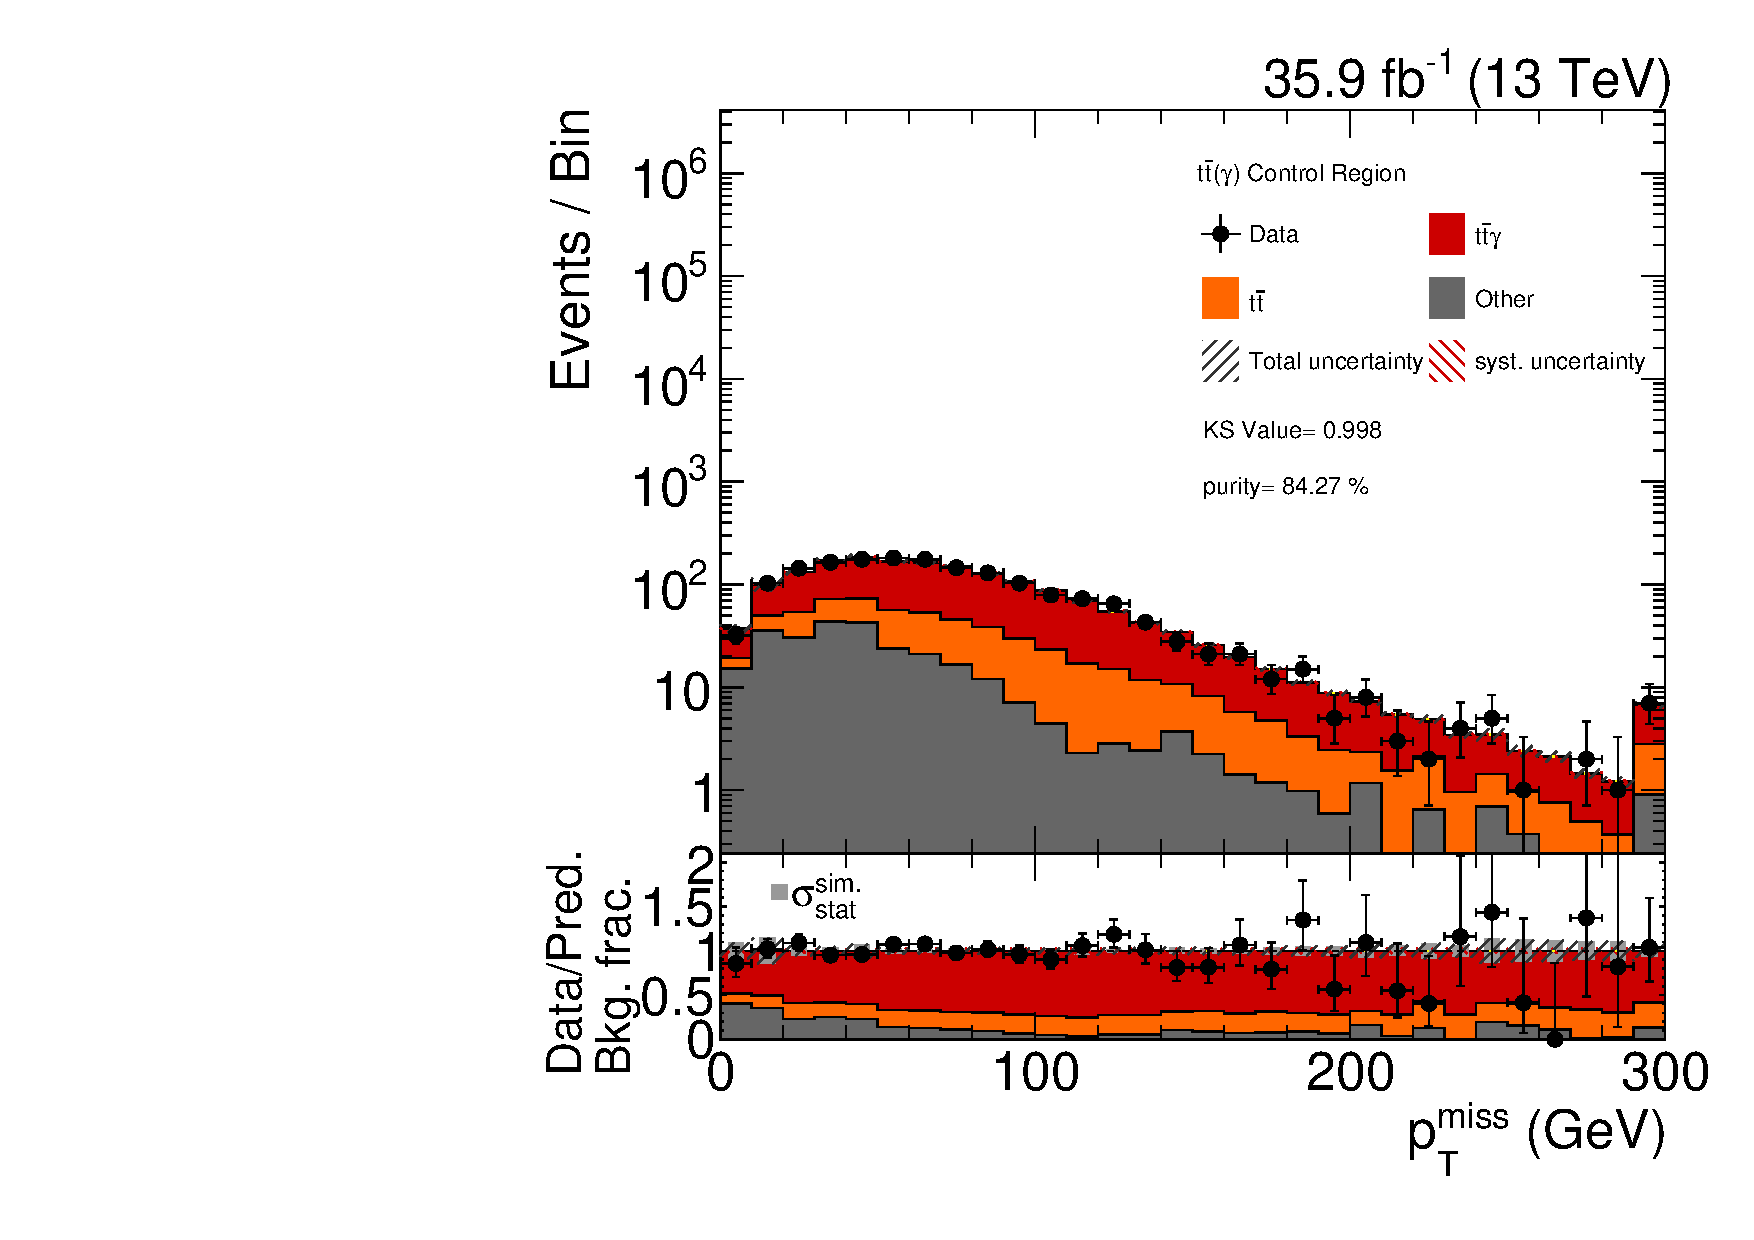
\includegraphics[width=\pairwidth]{figures/plots_CR_tt/CRTT_EM_nom_met_log}
 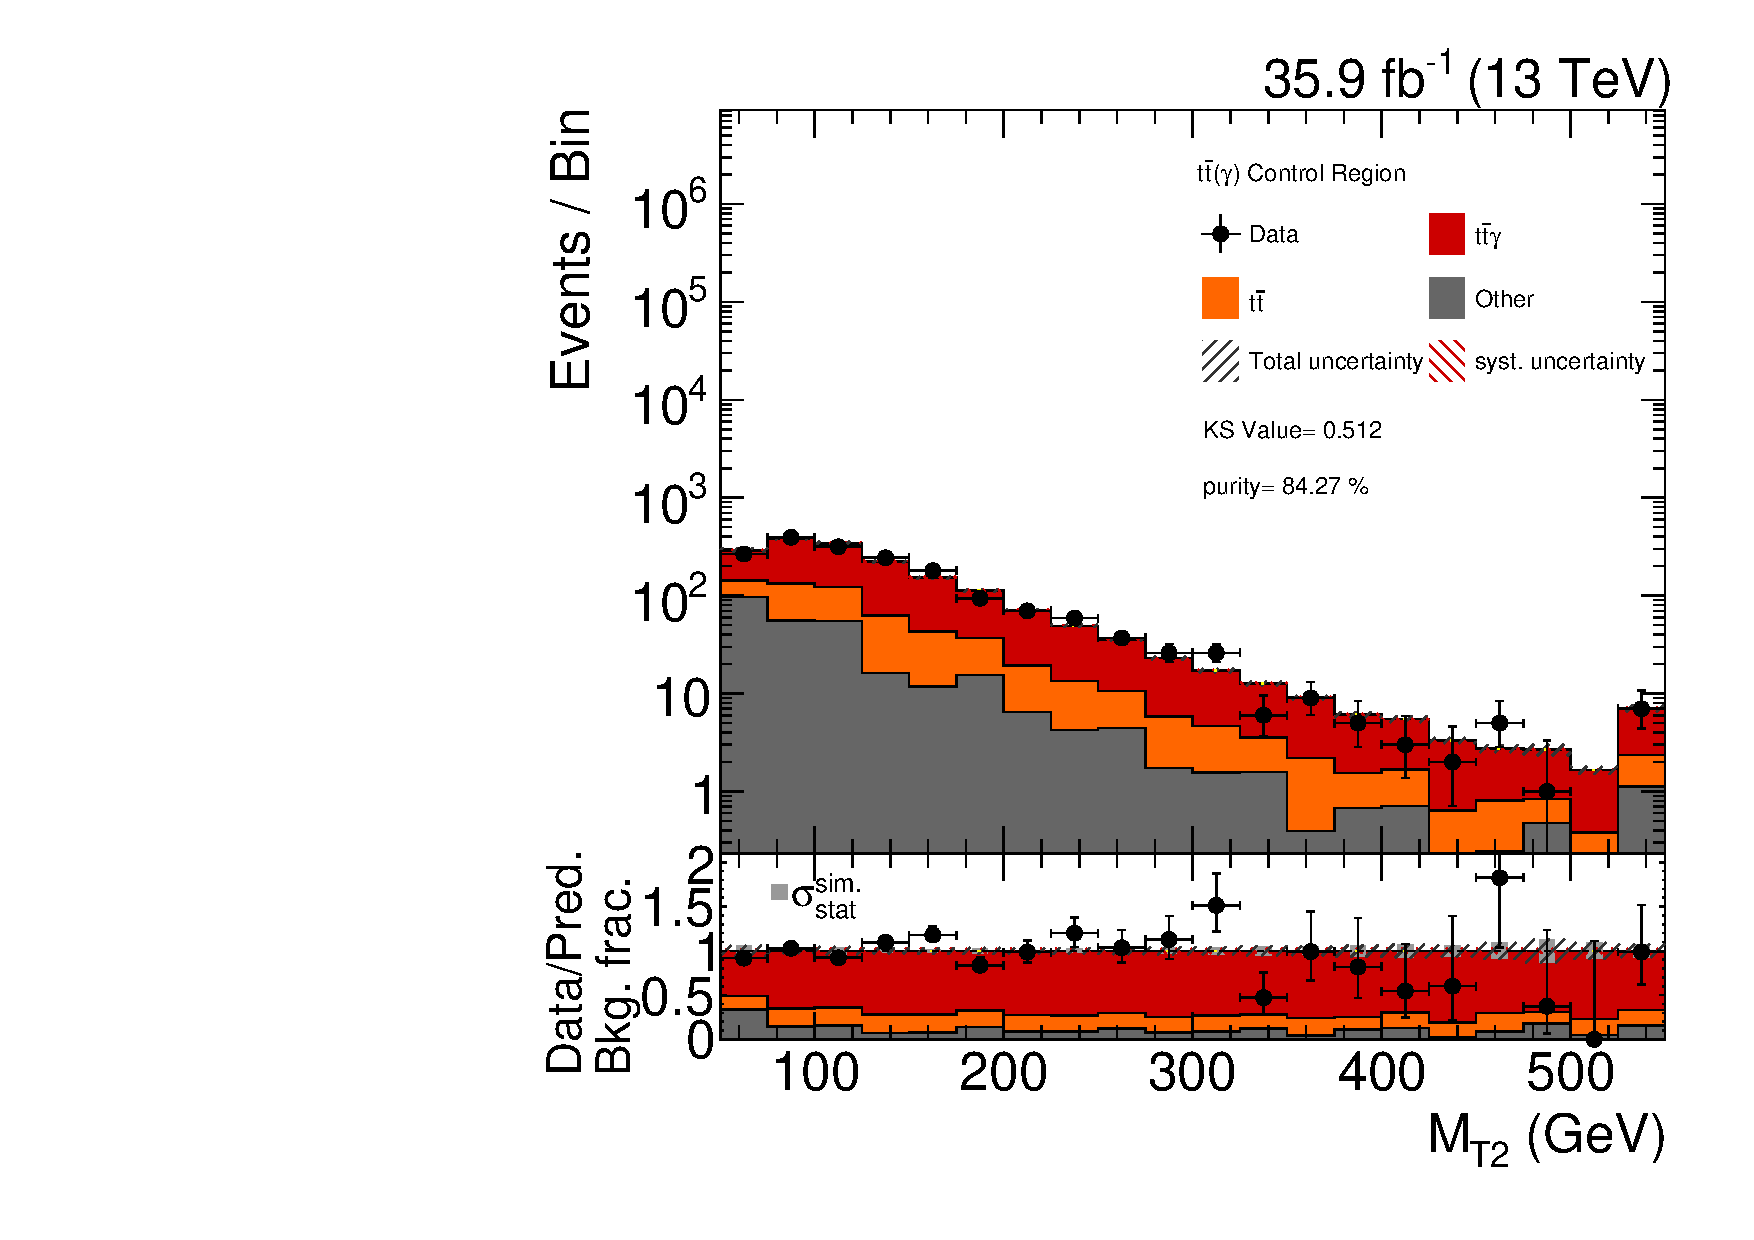
\includegraphics[width=\pairwidth]{figures/plots_CR_tt/CRTT_EM_nom_mt2_log}
 \caption{Comparisons between data and rescaled simulation in the $\ttbar(\PGg)$ CR in the $\ptmiss$ and $\mtTwo$ distribution. Below each plot, a ratio between data and prediction is shown. The uncertainty bands correspond to the systematic (red) and total uncertainty (gray). In addition, in the ratio plot the relative composition of the backgrounds is visualized. KS-values for the performed Kolmogorov-Smirnov test and the selection purity are also quoted.}
 \label{fig:CRTT}
\end{figure}
Additional statistical checks, such as Kolmogorov-Smirnov tests and $\chi^2$-fits, as explained above are also performed. The resulting KS-values of the Kolmogorov-Smirnov tests quoted in each plot indicate a good shape agreement.\\
The resulting curves of the $\chi^2$-fit distributions, see \refFig{fig:chiTT} left for an example fit in the $\ptmiss$ distribution, are smooth, indicating a proper performance of the fit. A comparison of all obtained SFs for the different setups and the SF obtained by the integral method is shown in \refFig{fig:chiTT} right. No significant deviation is observed, and all SFs are in agreement with each other. Hence, the scaling of the $\ttbar(\PGg)$ background seems stable and well described in the CR.
\begin{figure}[tbp]
 \centering
 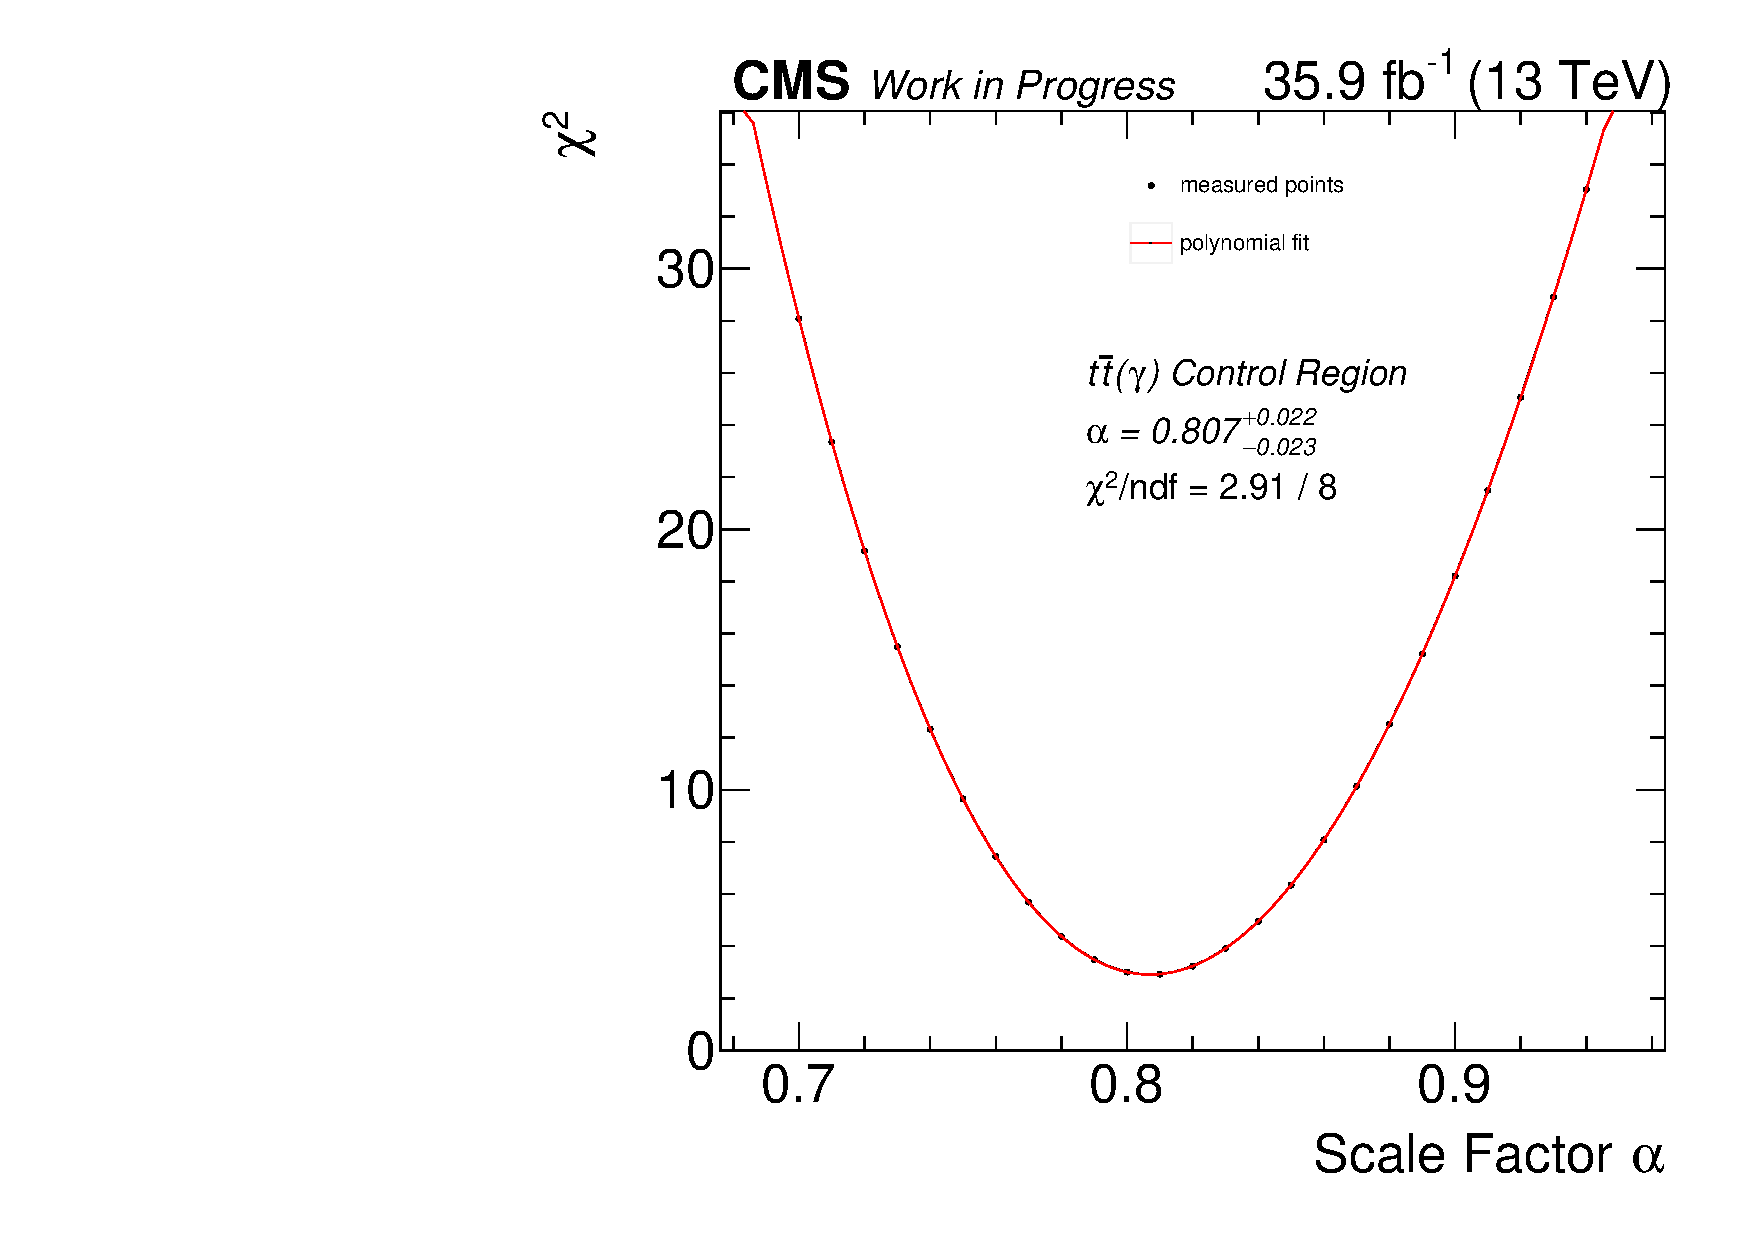
\includegraphics[width=\pairwidth]{figures/plots_CR/chi/TT_met}
 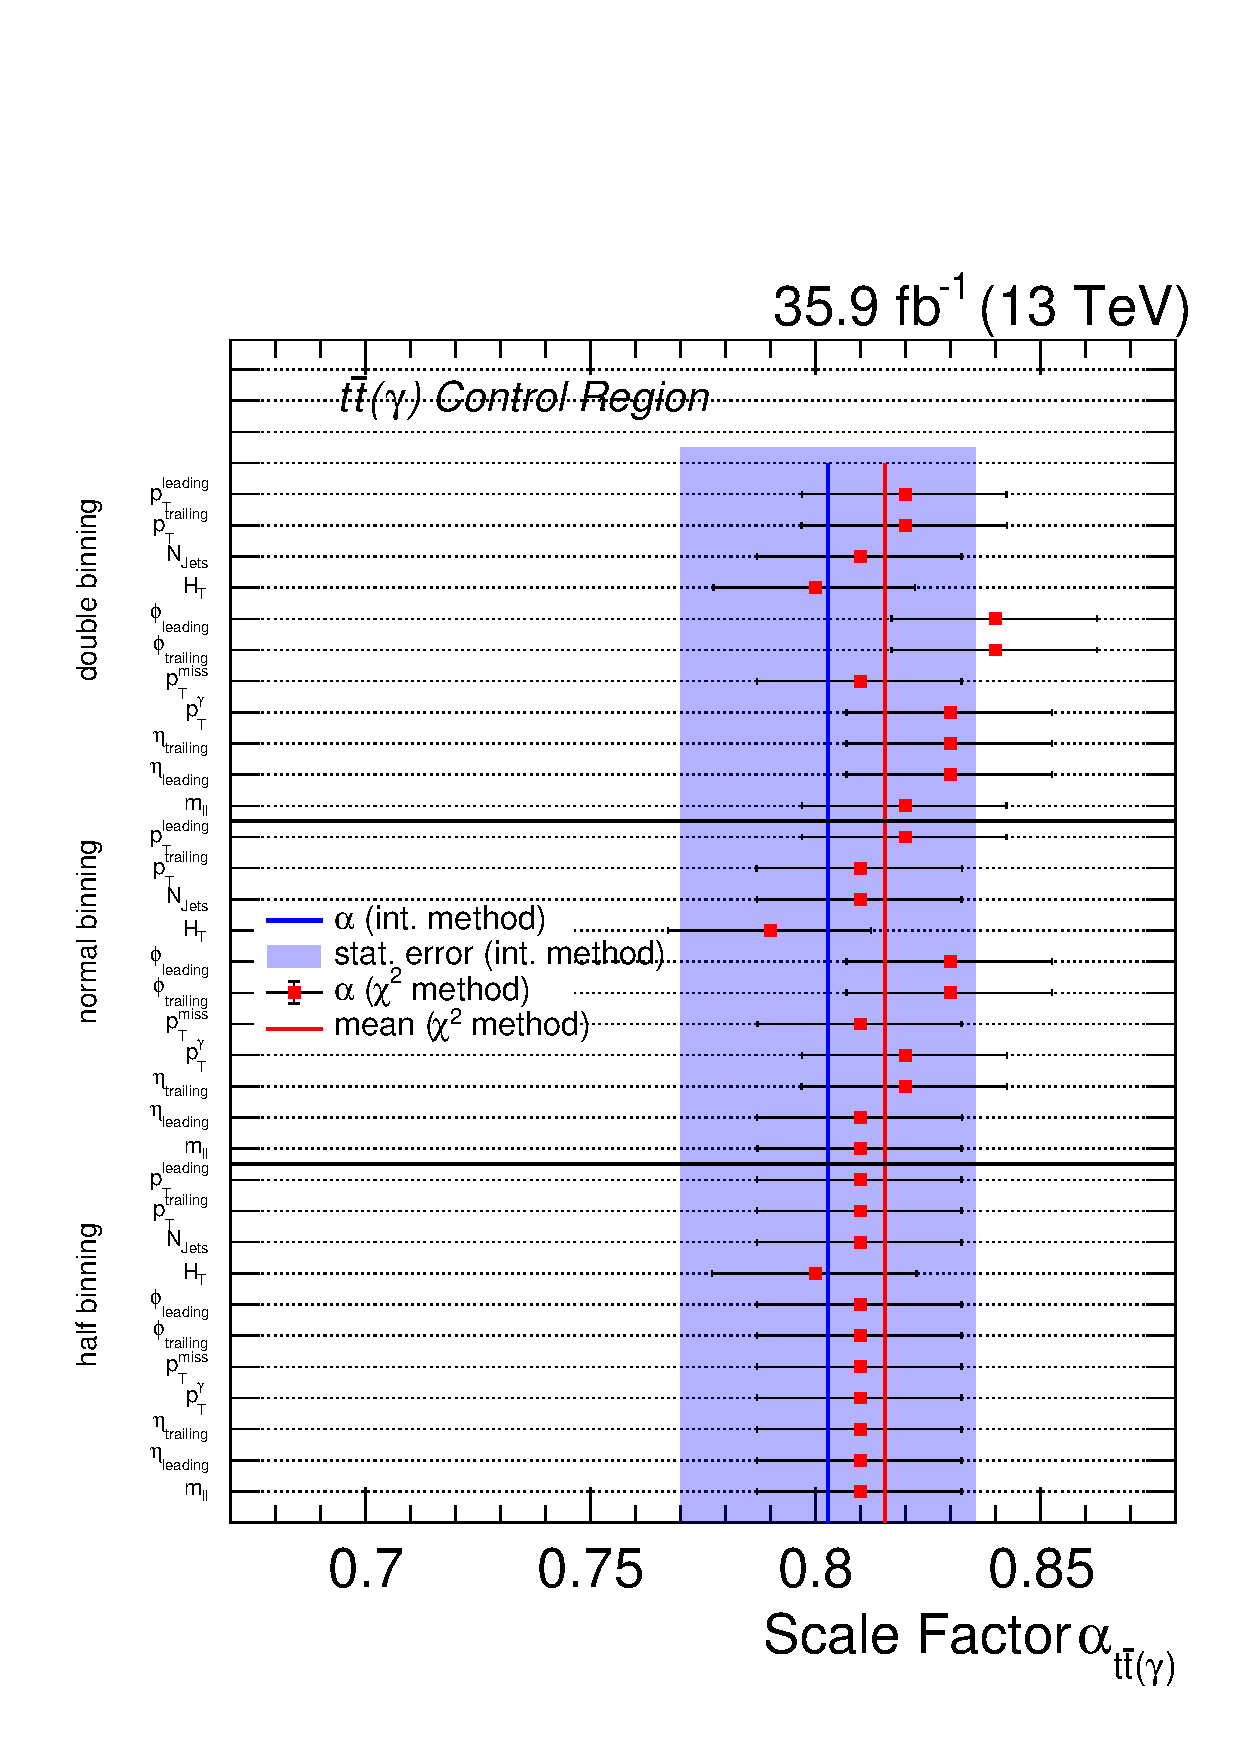
\includegraphics[width=\pairwidth]{figures/plots_CR/chi/TT_Compare}
 \caption{Example $\chi^2$-fit in the $\ttbar(\PGg)$ CR in the $\ptmiss$ distribution (left) with the polynomial fit. All fit results compared with the SF obtained from the integral method in different binnings and variables (right).}
 \label{fig:chiTT}
\end{figure}

\subsubsection*{Further studies}
Since the $\ttbar(\PGg)$ background is the most dominating one, further studies are performed in which the underlying MC simulation samples and their combination are examined. Different overlap removal procedures, see \refSec{sec:overlap}, and different available cross sections are used, while the fit procedure itself is varied. In addition, available corrections to improve the modeling of jet radiation in the initial state, and corrections to enhance the description of the top quark $\pt$ distribution, that are used both to correct the LO samples and the samples that are generated with \POWHEG (see~\refSec{sec:Simulation}), are applied in different combinations. The used fit methods include a $\chi^2$-template fit, where the ratio between the fractions of the $\ttbar$ and $\ttbar\PGg$ simulation is left free as an additional parameter, and a fit where only the $\ttbar\PGg$ simulation is made use of. The additional corrections to improve the modeling of the top quark $\pt$ distribution and the initial state jet radiation are observed to be unnecessary, because the modeling of the related distributions, \ie the jet multiplicity and the lepton $\pt$ distributions, is already in agreement with data in the standalone simulation. Using only the $\ttbar\PGg$ simulation yields the best agreement between simulated and observed shape, but is unphysical due to the missing $\ttbar$ process. For this reason, also the template fit method gives rise to similar results, since in the fit the $\ttbar\PGg$ sample has the highest impact due to the good shape agreement. Therefore, this approach is discarded, too. Eventually, no substantial differences are observed, and the best performance and stability is provided by the approach explained above.

\subsection{$\PW\PZ$ diboson production}
The diboson production of $\PW\PZ$ pairs is the second important background contribution for this analysis. It is also tuned to agree with the measurement in the $\PW\PZ$ CR, while the SF $\alpha_{\PW\PZ}$ is calculated with the integral method. The expected purity of selected $\PW\PZ$ events in this CR is about $84\%$.
% \begin{table}[tbp]
%  \centering
%  \caption{Yields in the $\PW\PZ$ CR for the pure simulation and measured data.}
%  \label{tab:CRWZ}
%  \begin{tabular}{llll}
%   process  & raw simulation & simulation & data                  \\\hline
%   $\PW\PZ$ & 113744         & 895.74     &                       \\\hline\hline
%   sum      & 113744         & 895.74     & \multirow{2}{*}{1193} \\
%   other    & 93914          & 173.47     &
%  \end{tabular}
% \end{table}
% The agreement beforehand is also very good, considering this background is a higher order process and is therefore simulated at NLO, see \refSec{sec:Simulation}, which includes several complicated effects the event generator needs to handle properly.
The SF $\alpha_{\PW\PZ}$ is determined to be
\begin{equation}\label{eq:AlphaWZ}
 \alpha_{\PW\PZ}=1.14 \pm 0.04 (stat.) [\hat{=}3.2\%].
\end{equation}
Higher order effects can lead to larger cross sections as calculated within the NLO simulation, thus it is not unexpected to obtain a SF varying $\approx12\%$ from unity. Resulting distributions of the description of the $\ptmiss$ and $\mtTwo$ variables are shown in \refFig{fig:CRWZ}. As can be seen, the predicted shape is in consistency over the whole range with the observed data, also in the high $\ptmiss$ and $\mtTwo$ regime. This is further confirmed by the additional cross checks, that are also realized in the $\ttbar(\PGg)$ CR described above. The KS-values close to one strengthen the trust in the background estimation method.
% The comparison plots for other distributions can be found in the appendix in \refFig{fig:app_}.
\begin{figure}[tbp]
 \centering
 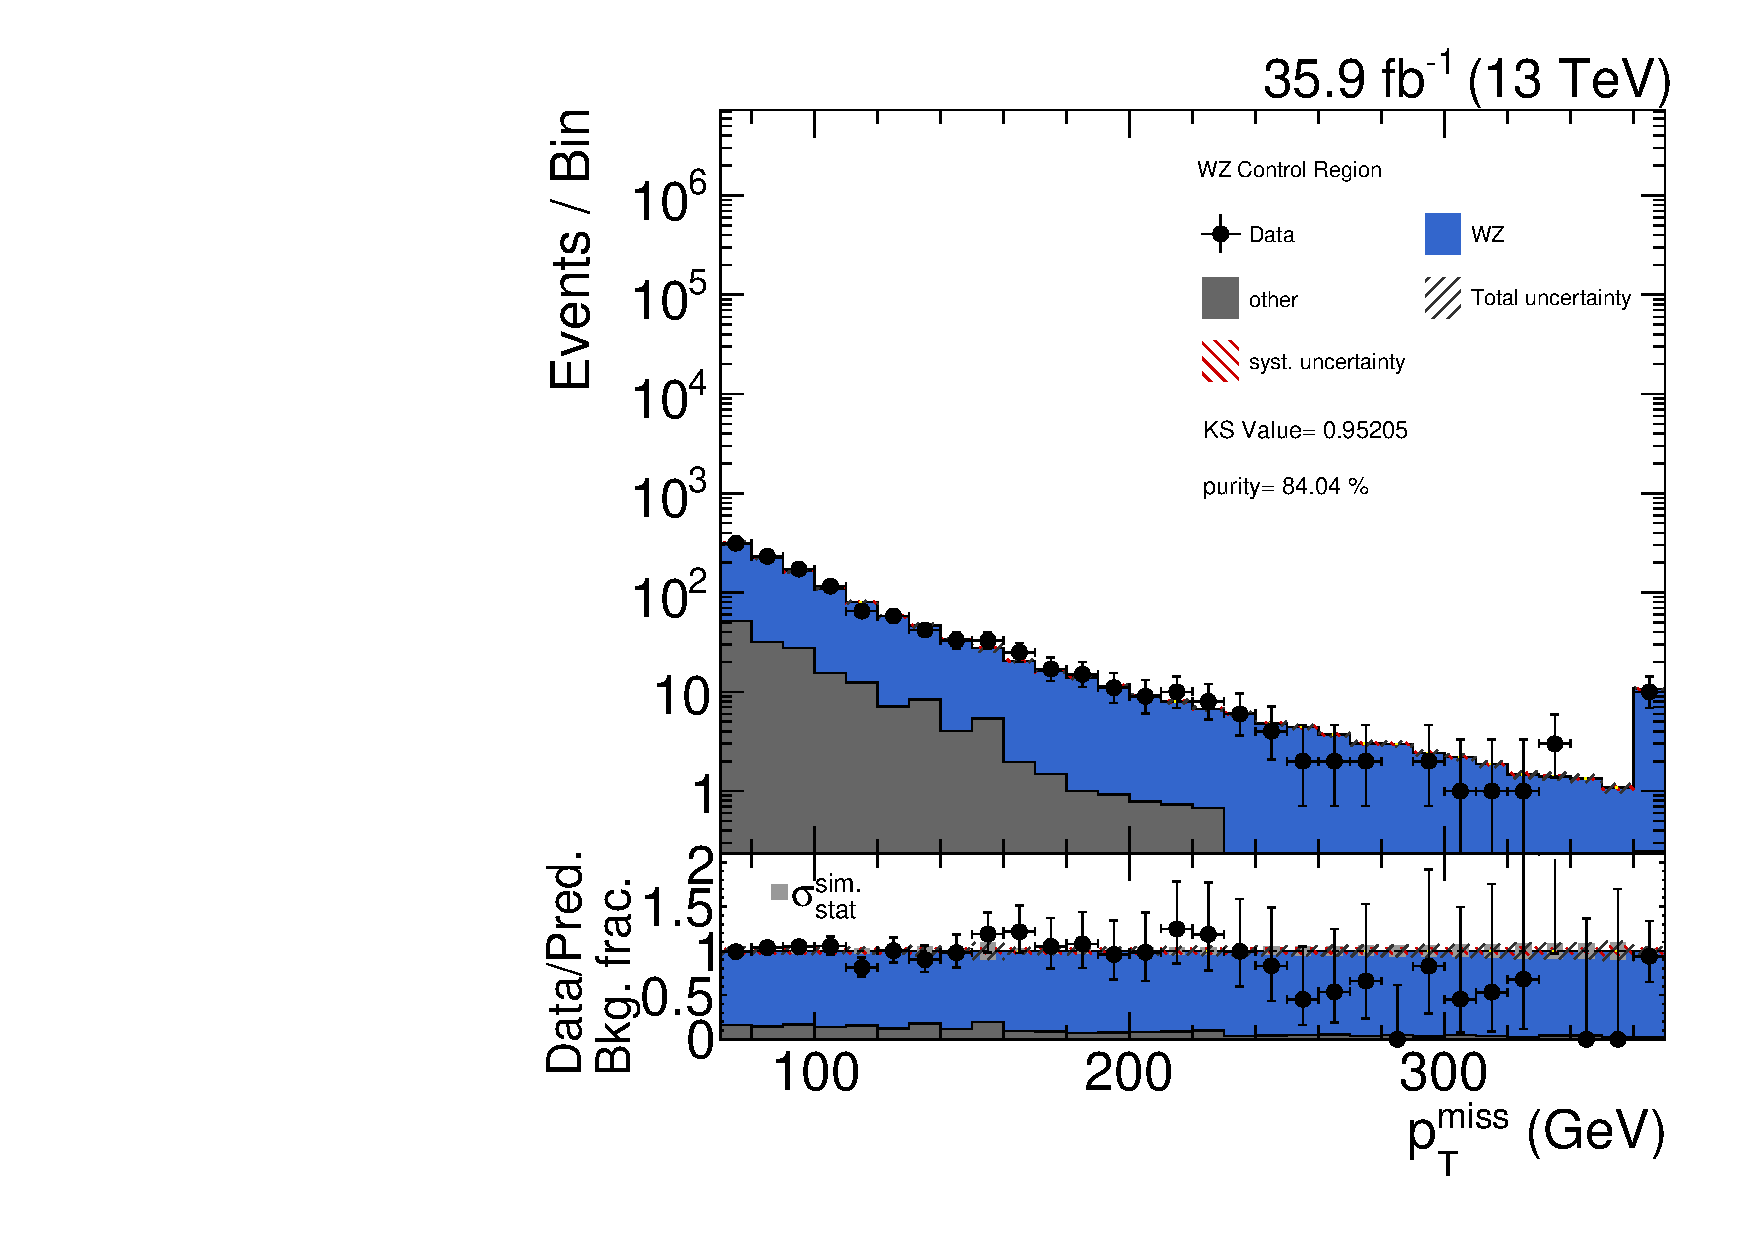
\includegraphics[width=\pairwidth]{figures/plots_CR_wz/CRWZ_LL_nom_met_log}
 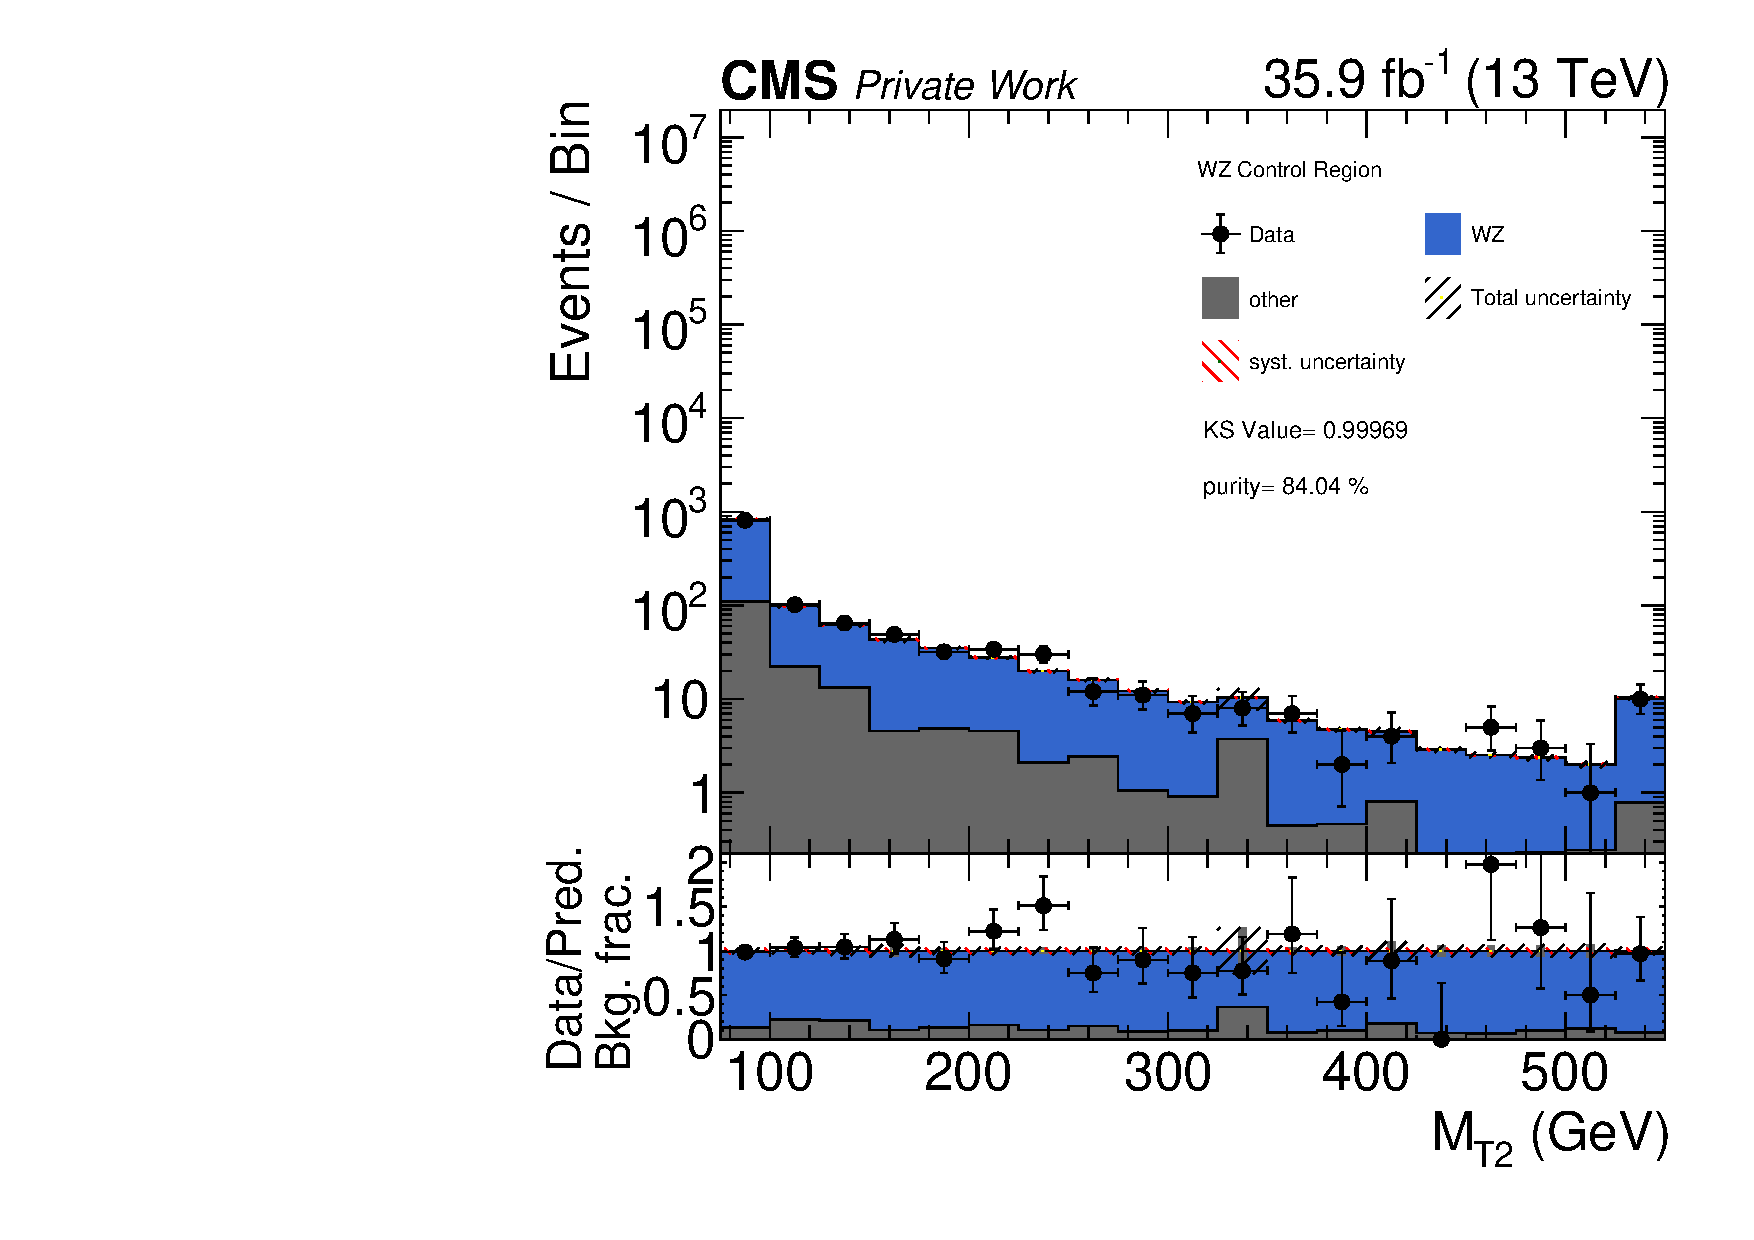
\includegraphics[width=\pairwidth]{figures/plots_CR_wz/CRWZ_LL_nom_mt2_log}
 \caption{Comparisons between data and rescaled simulation in the $\PW\PZ$ CR in the $\ptmiss$ and $\mtTwo$ distribution. Below each plot, a ratio between data and prediction is shown. The uncertainty bands correspond to the systematic (rand) and total uncertainty (gray). In addition, in the ratio plot the relative composition of the backgrounds is visualized. KS-values for the performed Kolmogorov-Smirnov test and the selection purity are also quoted.}
 \label{fig:CRWZ}
\end{figure}
The $\chi^2$-fit studies lead to the same outcome as can be seen in \refFig{fig:chiWZ}.
% The $\chi^2$-fit studies lead to the same outcome as can be seen in \refFig{fig:chiWZ} right. Each individual $\chi^2$-fit seems to behave properly, see \refFig{fig:chiWZ} (left) for an example in the $\ptmiss$ distribution.

\begin{figure}[tbp]
 \centering
 % 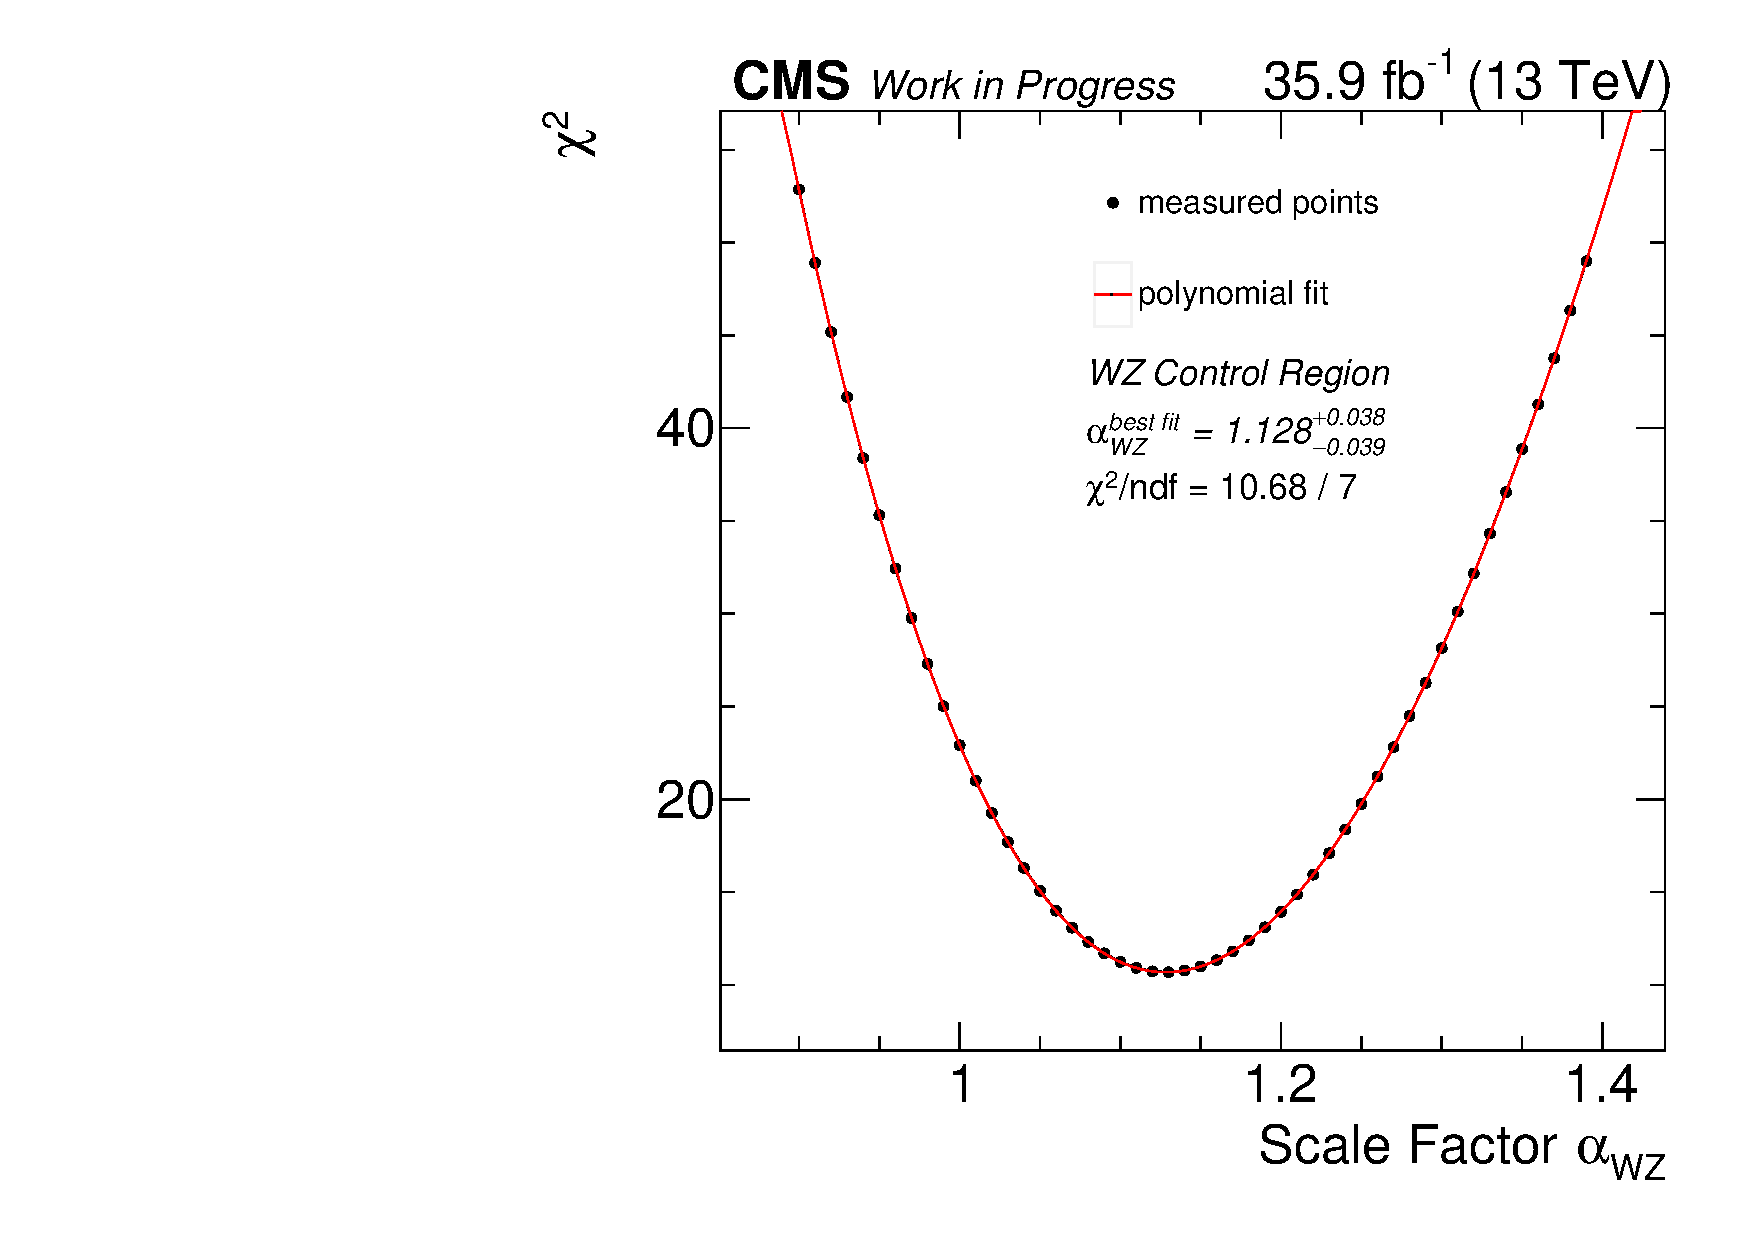
\includegraphics[width=\pairwidth]{figures/plots_CR/chi/WZ_met}
 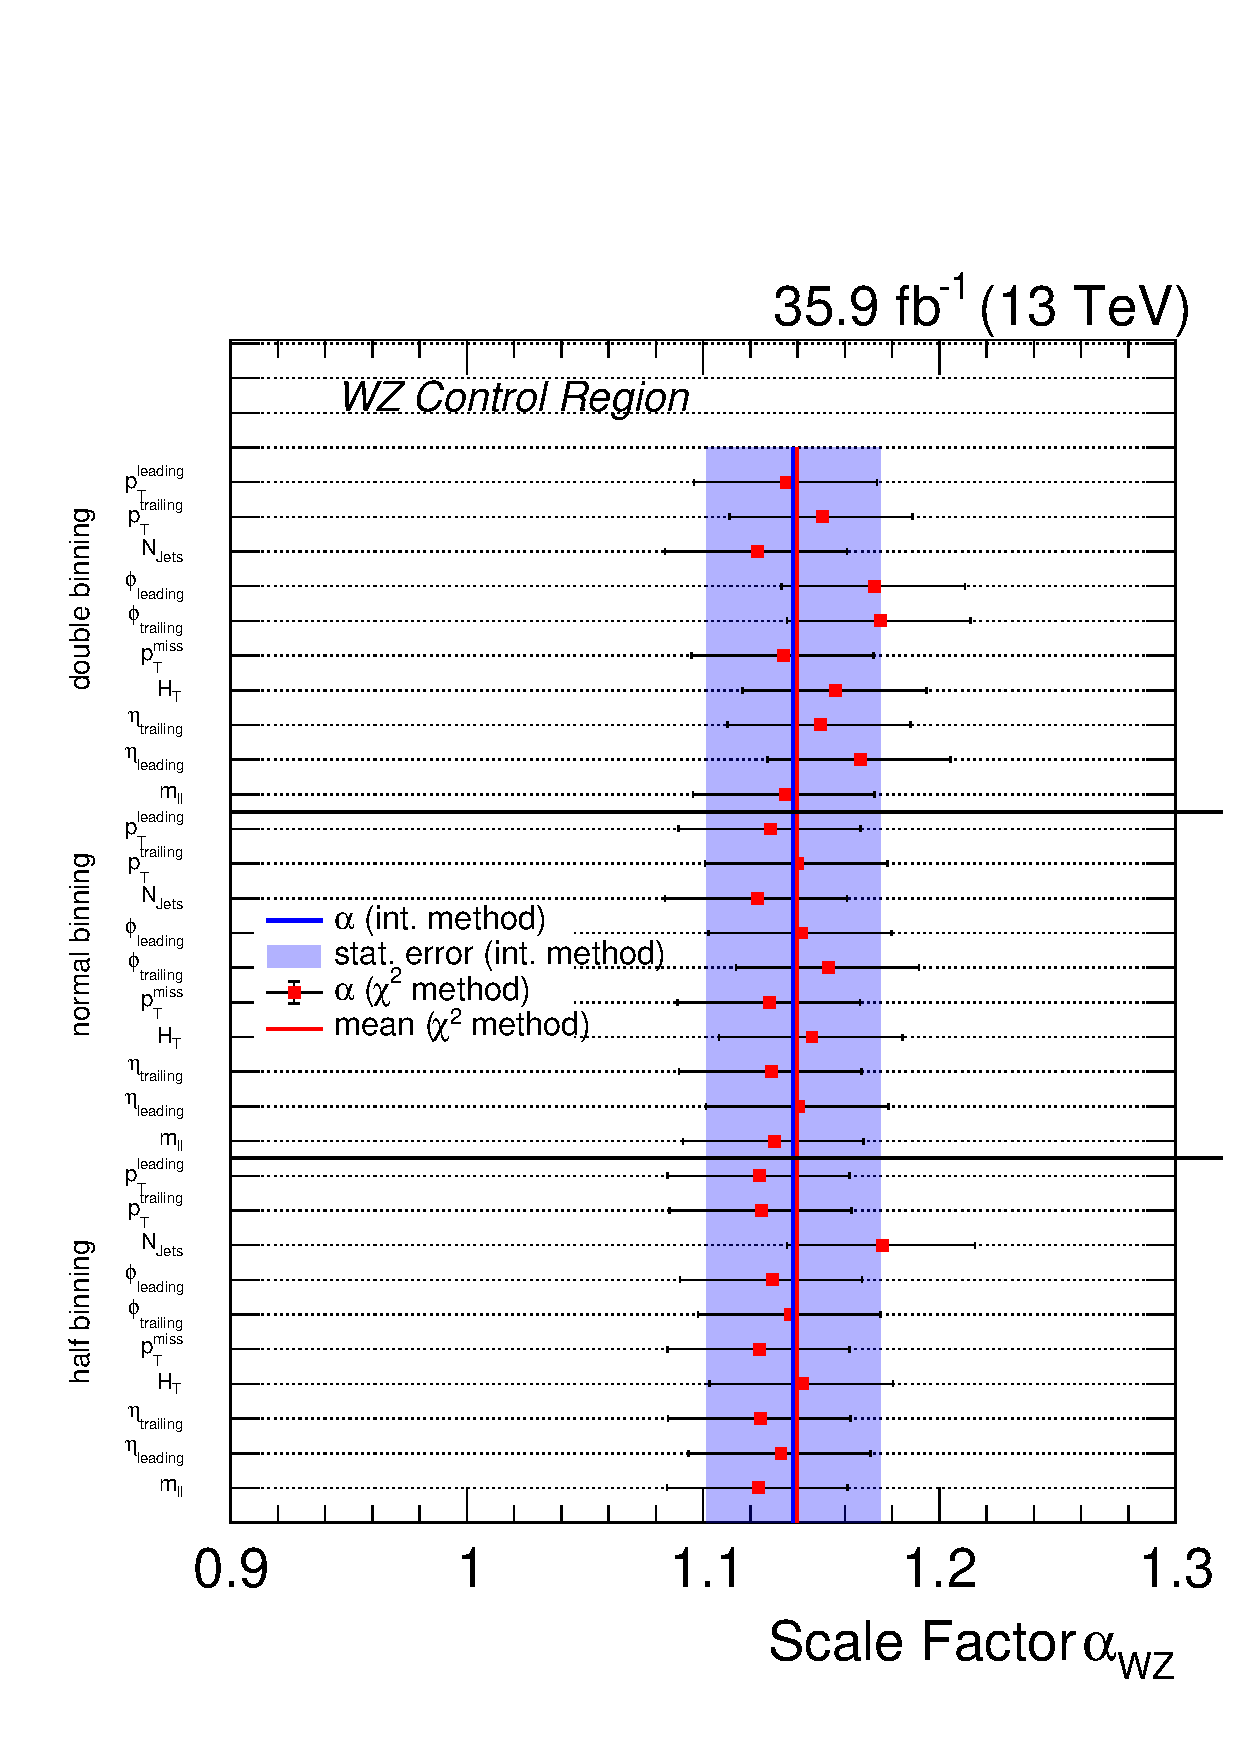
\includegraphics[width=\pairwidth]{figures/plots_CR/chi/WZ_Compare}
 \caption{All $\chi^2$-fit results compared with the SF obtained from the integral method in different binnings and variables.}
 % \caption{Example $\chi^2$-fit in the $\PW\PZ$ CR in the $\ptmiss$ distribution (left) with the polynomial fit. All fit results compared with the SF obtained from the integral method in different binnings and variables (right).}
 \label{fig:chiWZ}
\end{figure}




\subsection{$\PZ\PZ$ diboson production}
The third biggest background contribution is $\PZ\PZ$ diboson production, where both Z bosons decay leptonically, one to charged leptons such as electrons or muons, and the other one to neutrinos. To simplify the construction of a dedicated CR, as explained in \refSec{sec:CR}, the simulation procedure is exploitet. Since the simulation of the events is the same for both charged leptons and neutrinos for the Z boson decays due to the identical generator, only the detector response differs. Therefore, $\PZ\PZ$ can be well estimated in a four lepton CR. A pure selection of $\PZ\PZ$ events can be established, although the statistics in data is quite low due to small cross section and the low branching fraction for the $\Z\to\ell\ell$ decay. The selection purity is nearly $100\%$.
% Event counts are quoted in \refTab{tab:CRZZ}, with a selection purity of nearly $100\%$.
% \begin{table}[tbp]
%  \centering
%  \caption{Yields in the $\PZ\PZ$ CR for the pure simulation and measured data.}
%  \label{tab:CRZZ}
%  \begin{tabular}{llll}
%
%   process                 & raw simulation & simulation & data                 \\\hline
%   $\PZ\PZ(\to2\ell2\Pgn)$ & 5              & 0.0005     &                      \\
%   $\PZ\PZ(\to4\ell)$      & 459221         & 226.94     &                      \\\hline\hline
%   sum                     & 459226         & 226.94     & \multirow{2}{*}{251} \\
%   other                   & 74             & 1.48       &
%  \end{tabular}
% \end{table}
With the integral method applied, the SF $\alpha_{\PZ\PZ}$ is given by
\begin{equation}\label{eq:AlphaZZ}
 \alpha_{\PZ\PZ}=1.109 \pm 0.064 (stat.) [\hat{=}5.74\%].
\end{equation}
Post-fit distributions in the $\ptmiss$ distribution and invariant dilepton mass distribution of the second Z boson can be found in \refFig{fig:CRZZ}. As mentioned, the precision is limited by the low statistics of the selected sample, but nevertheless is sufficient enough to establish a stable background prediction. The shapes agree well, as it is additionally indicated by the KS-values printed on the plots. The properties of the $\PZ\PZ\to4\ell$ process does not allow to study the prediction in the high $\ptmiss$ regime, since only nongenuine $\ptmiss$ is produced. However, based on the agreement of distributions of the third and fourth leptons, such as $m_{\ell_3\ell_4}$, and the agreement of the description of nongenuine $\ptmiss$, the agreement of $\ptmiss$ in the $\PZ\PZ\to2\ell2\PGn$ background can be assumed.
\begin{figure}[tbp]
 \centering
 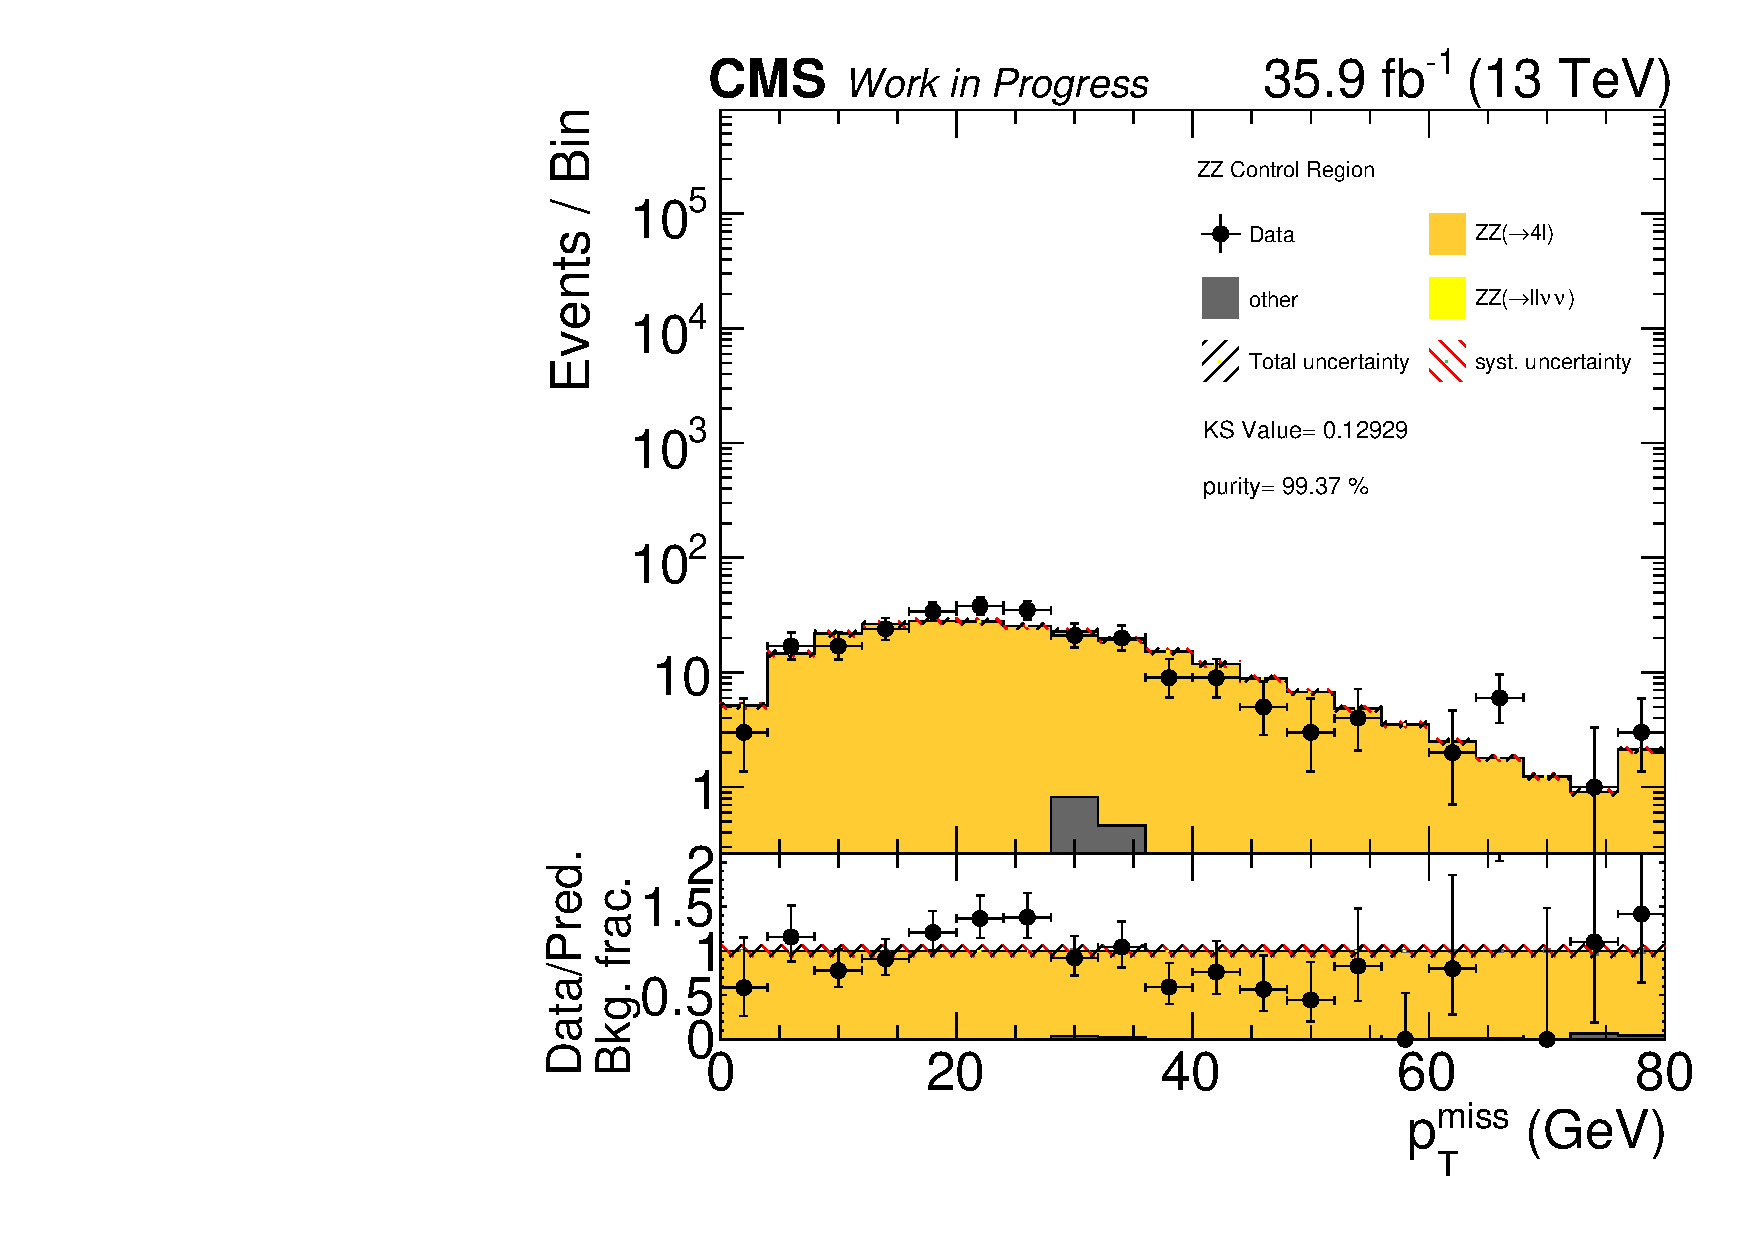
\includegraphics[width=\pairwidth]{figures/plots_CR_zz/CRZZ_LL_nom_met_log}
 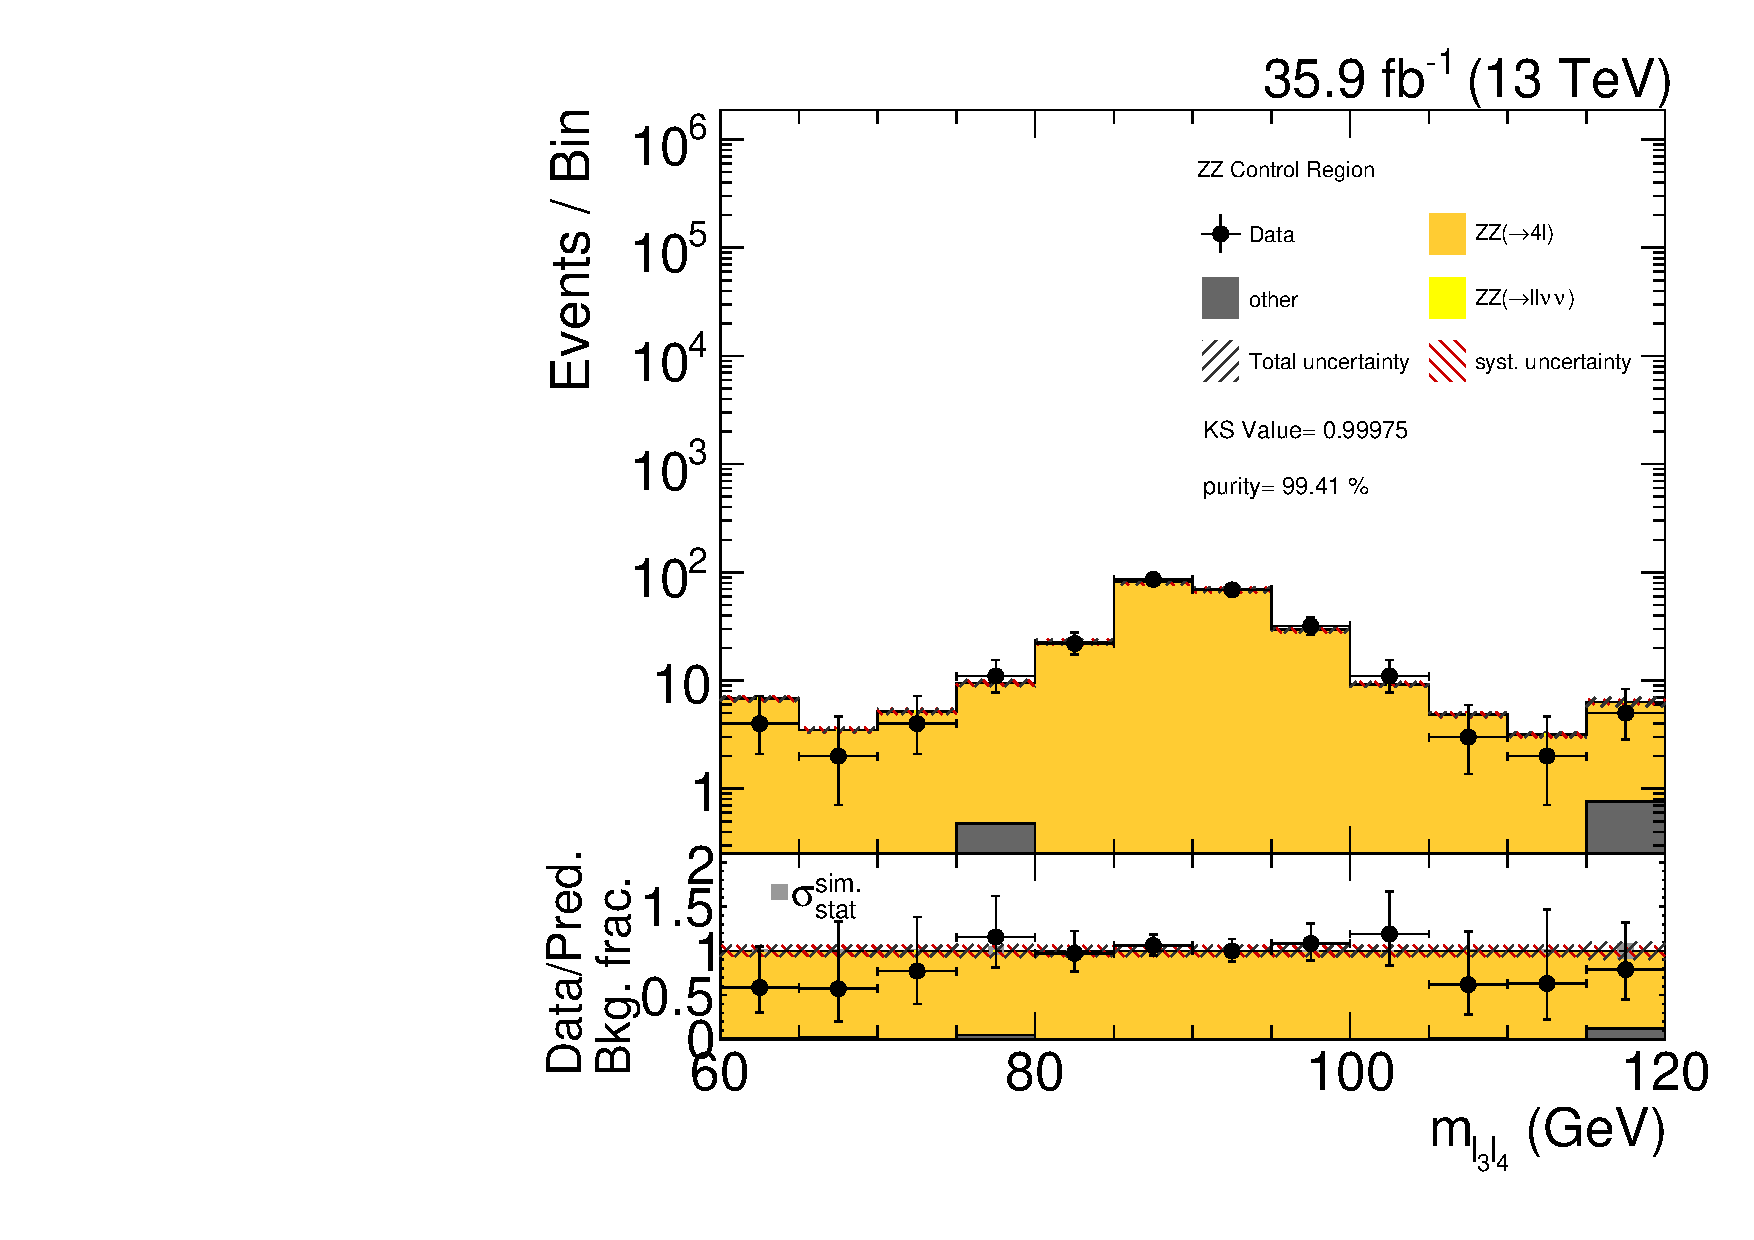
\includegraphics[width=\pairwidth]{figures/plots_CR_zz/CRZZ_LL_nom_m_ll2_log}
 \caption{Comparisons between data and rescaled simulation in the $\PZ\PZ$ CR in the $\ptmiss$ and $m_{\ell_3\ell_4}$ distribution. Below each plot, a ratio between data and prediction is shown. The uncertainty bands correspond to the systematic (red) and total uncertainty (gray). In addition, in the ratio plot the relative composition of the backgrounds is visualized. KS-values for the performed Kolmogorov-Smirnov test and the selection purity are also quoted.}
 \label{fig:CRZZ}
\end{figure}
The $\chi^2$-fit studies, see \refFig{fig:chiZZ}, are performed as for the other three background estimations discussed above, and yield the same conclusion, although some fluctuations in the choice of the variable or binning are present due to the lower total event count in the observed data. All in all also this background estimation method is stable.
\begin{figure}[tbp]
 \centering
 % 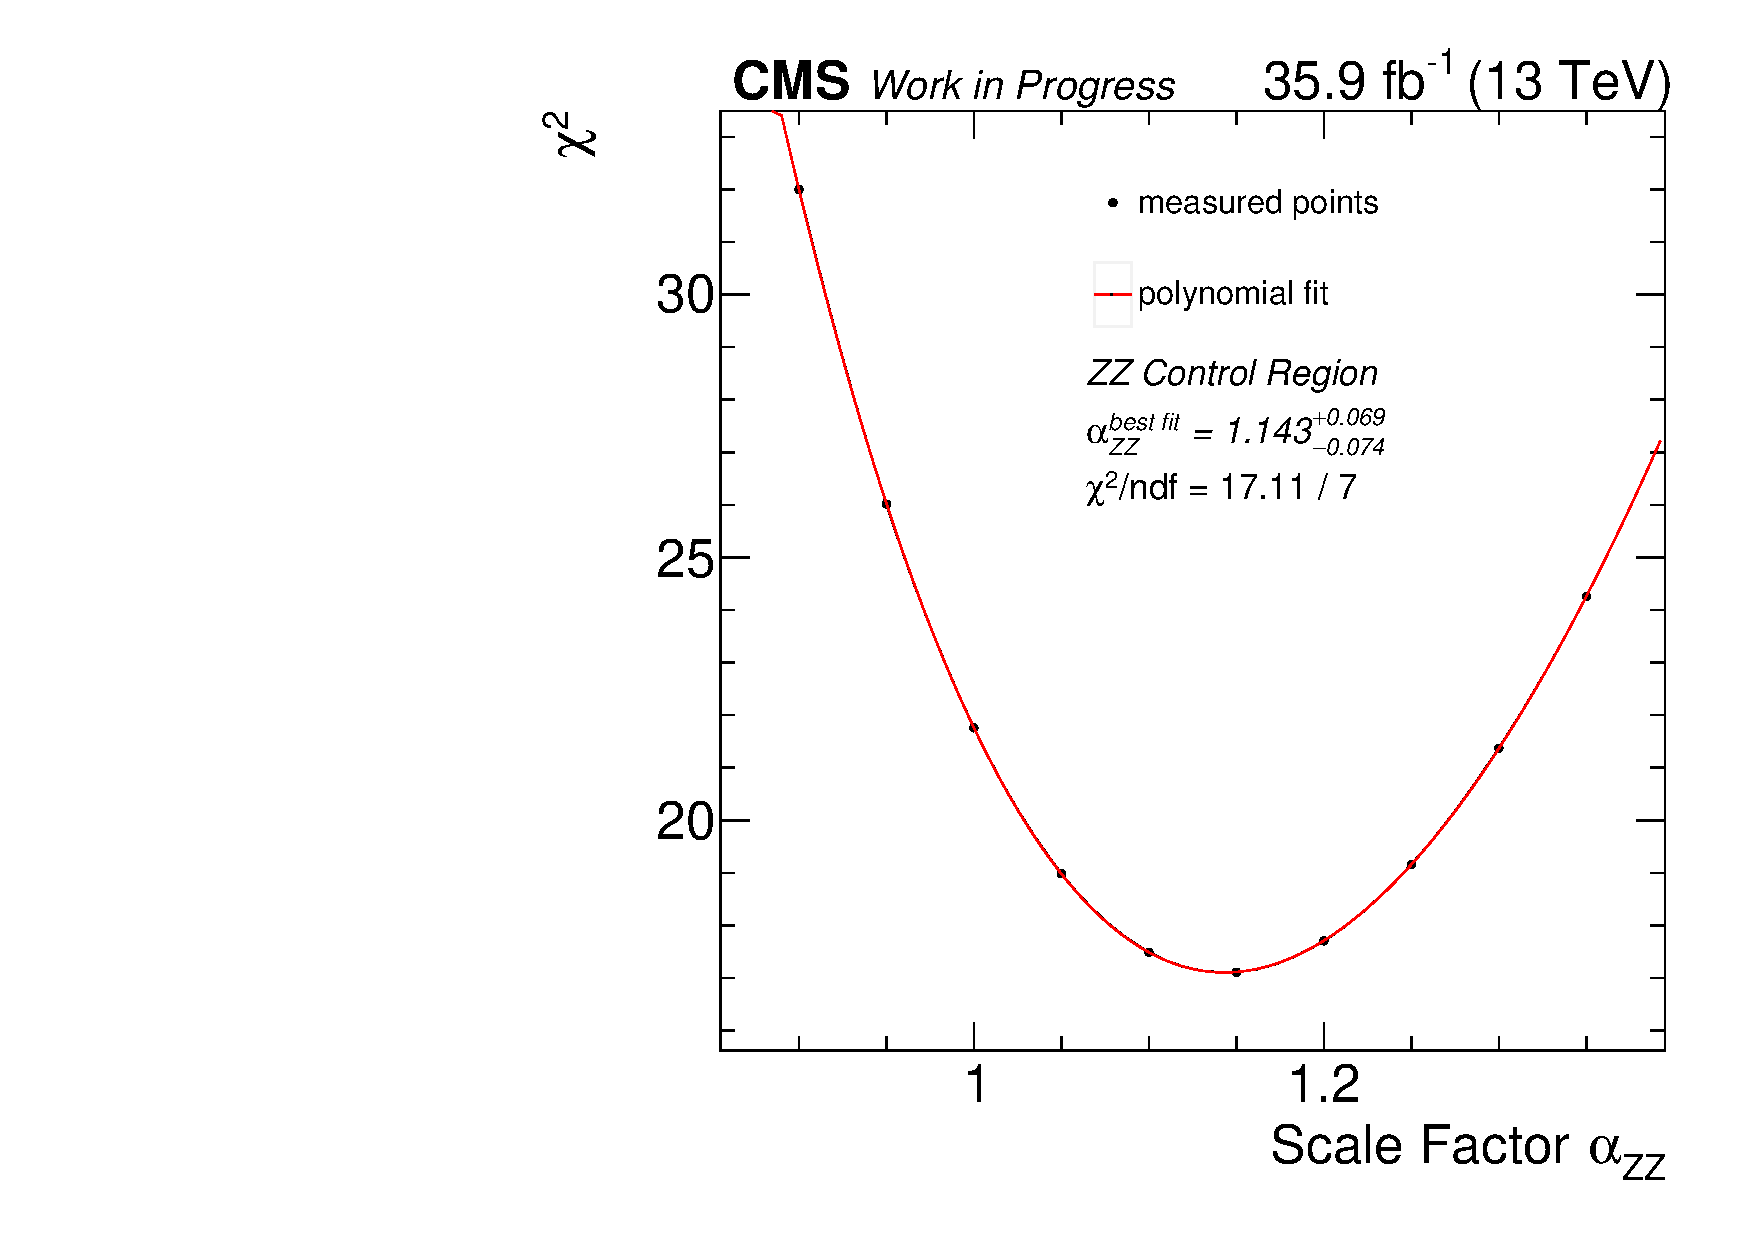
\includegraphics[width=\pairwidth]{figures/plots_CR/chi/ZZ_met}
 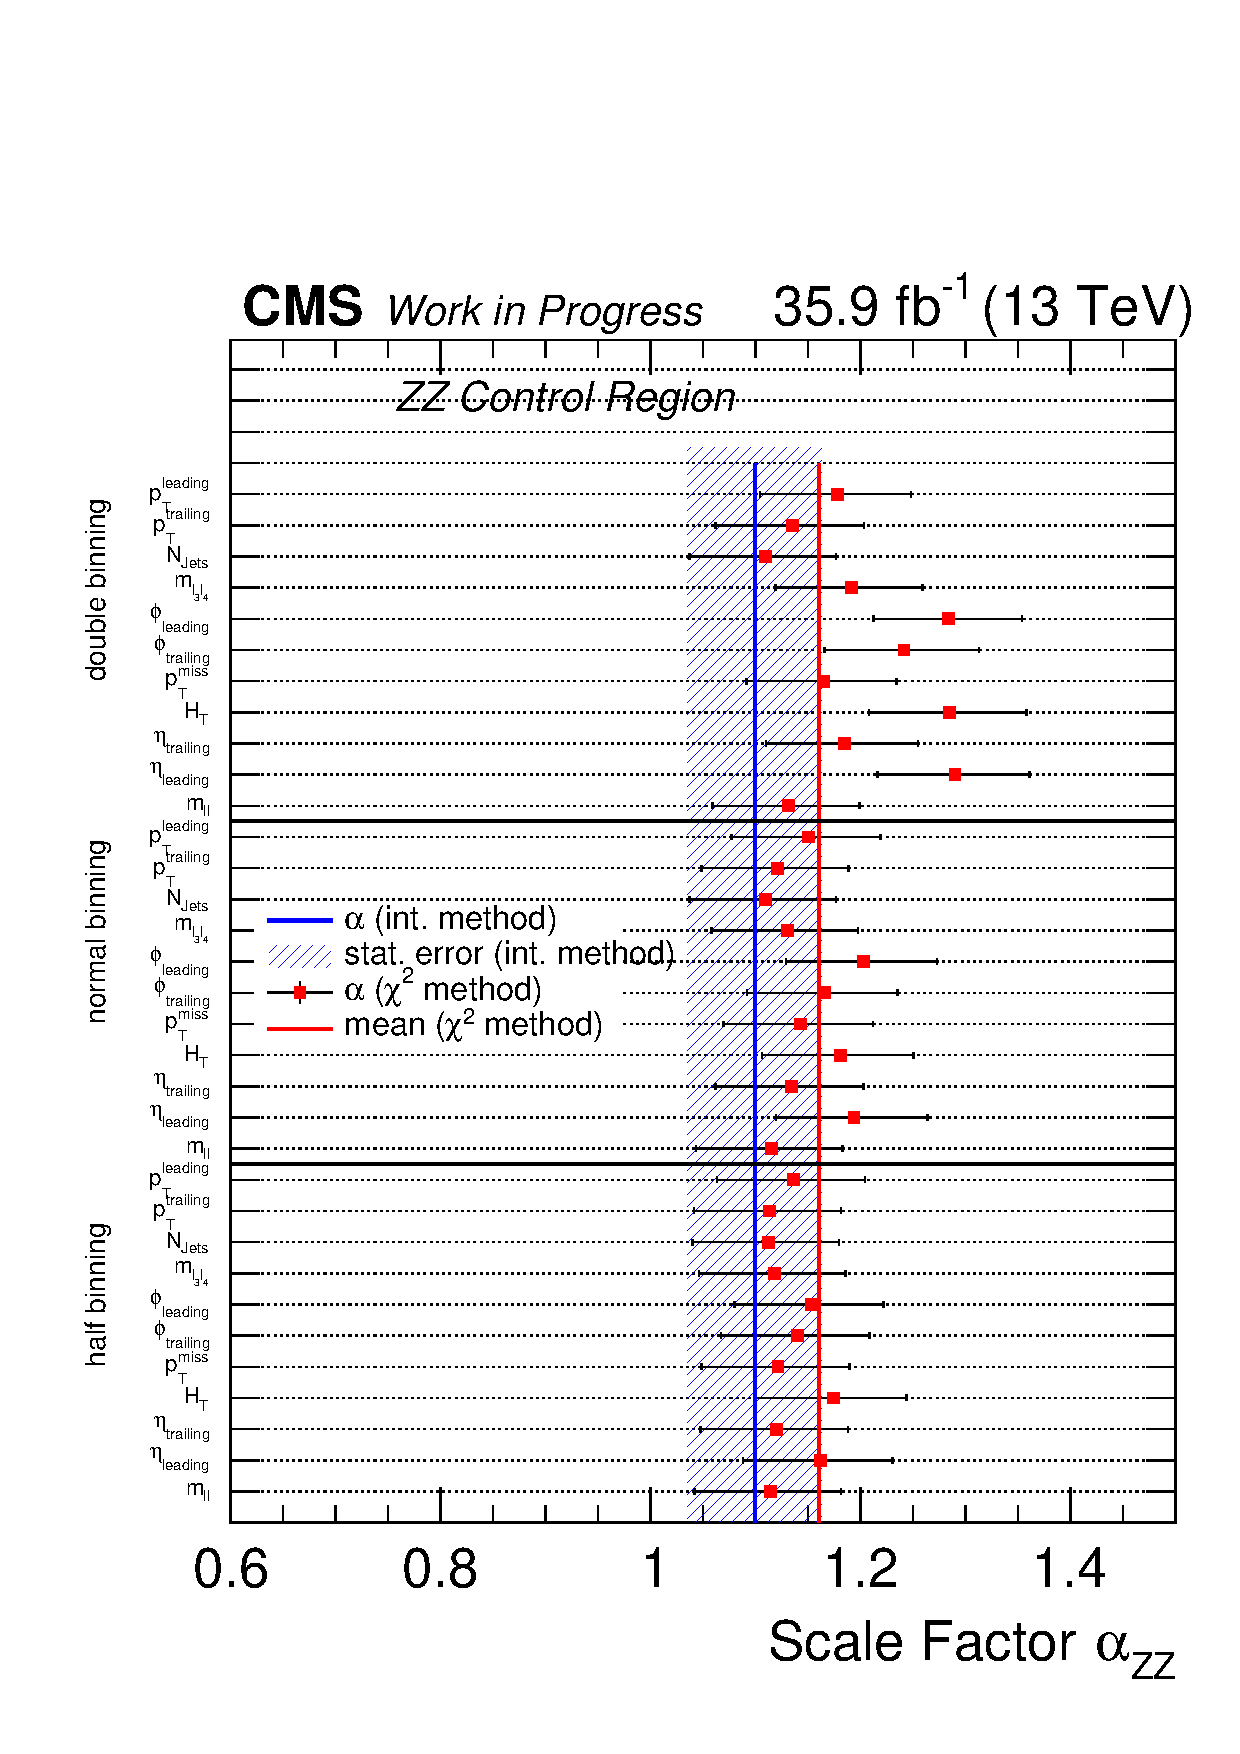
\includegraphics[width=\pairwidth]{figures/plots_CR/chi/ZZ_Compare}
 \caption{All $\chi^2$-fit results compared with the SF obtained from the integral method in different binnings and variables.}
 % \caption{Example $\chi^2$-fit in the $\PZ\PZ$ CR in the $\ptmiss$ distribution (left) with the polynomial fit. All fit results compared with the SF obtained from the integral method in different binnings and variables (right).}
 \label{fig:chiZZ}
\end{figure}

\subsection{Drell-Yan and $\PZ\PGg$ production}
Although contribution from the Drell-Yan and $\PZ\PGg$ backgrounds is small in the two SR bins, its contribution is the fourth largest. As in the case of the $\ttbar(\PGg)$ background, it is composed of two major parts, the Drell-Yan process, where quarks annihilate to off-shell photons or Z bosons and generate leptons in their decays, and the diboson production of $\PZ\PGg$. The integral method as explained above is used to determine the SF $\alpha_{DY/\PZ(\PGg)}$ in the dedicated CR defined in \refSec{sec:CR}.
% The relevant event yields are quoted in \refTab{tab:CRDY}, and t
The resulting SF is stated in \refEq{eq:AlphaDY}. With a purity of about $99\%$, and a large total event count, a precise SF determination is feasible, as can be concluded also from the small statistical uncertainty of around $1\%$. The agreement between simulation and data is very good even before application of $\alpha_{DY/\PZ(\PGg)}$, since the SF equals nearly unity. The post-scaling distributions of $\ptmiss$ and $\mtTwo$ are shown in \refFig{fig:CRDY}. They show overall a good agreement, only in the high $\mtTwo$ region there are some fluctuations due to the limited statistics being present both in data and simulation.
% Further distributions are investigated, that can be found in the appendix in \refFig{fig_app}.
Most of the KS-values indicate a very good matching between predicted and observed shape, albeit the Kolmogorov-Smirnov test provides a very small KS value for the consistency between the $\ptmiss$ distributions. This is mainly due to the high statistics in data and therefore a higher absolute discrepancy, in contradiction to the lower statistics in simulation, leading to larger fluctuations. These discrepancy is also visible in the ratio in the bottom panel of the plot, but is consistent with the shown total uncertainty.\\
% \begin{table}[tbp]
%  \centering
%  \caption{Yields in the DY/$\PZ(\PGg)$ CR for the pure simulation and measured data.}
%  \label{tab:CRDY}
%  \begin{tabular}{llll}
%
%   process   & raw simulation & simulation & data                   \\\hline
%   Drell-Yan & 11710          & 13008.53   &                        \\
%   $\PZ\PGg$ & 170161         & 22692.88   &                        \\\hline\hline
%   sum       & 181871         & 35701.41   & \multirow{2}{*}{38419} \\
%   other     & 87337          & 377.02     &
%  \end{tabular}
% \end{table}
\begin{equation}\label{eq:AlphaDY}
 \alpha_{DY/\PZ(\PGg)}=1.066 \pm 0.001 (stat.) [\hat{=}0.87\%].
\end{equation}

\begin{figure}[tbp]
 \centering
 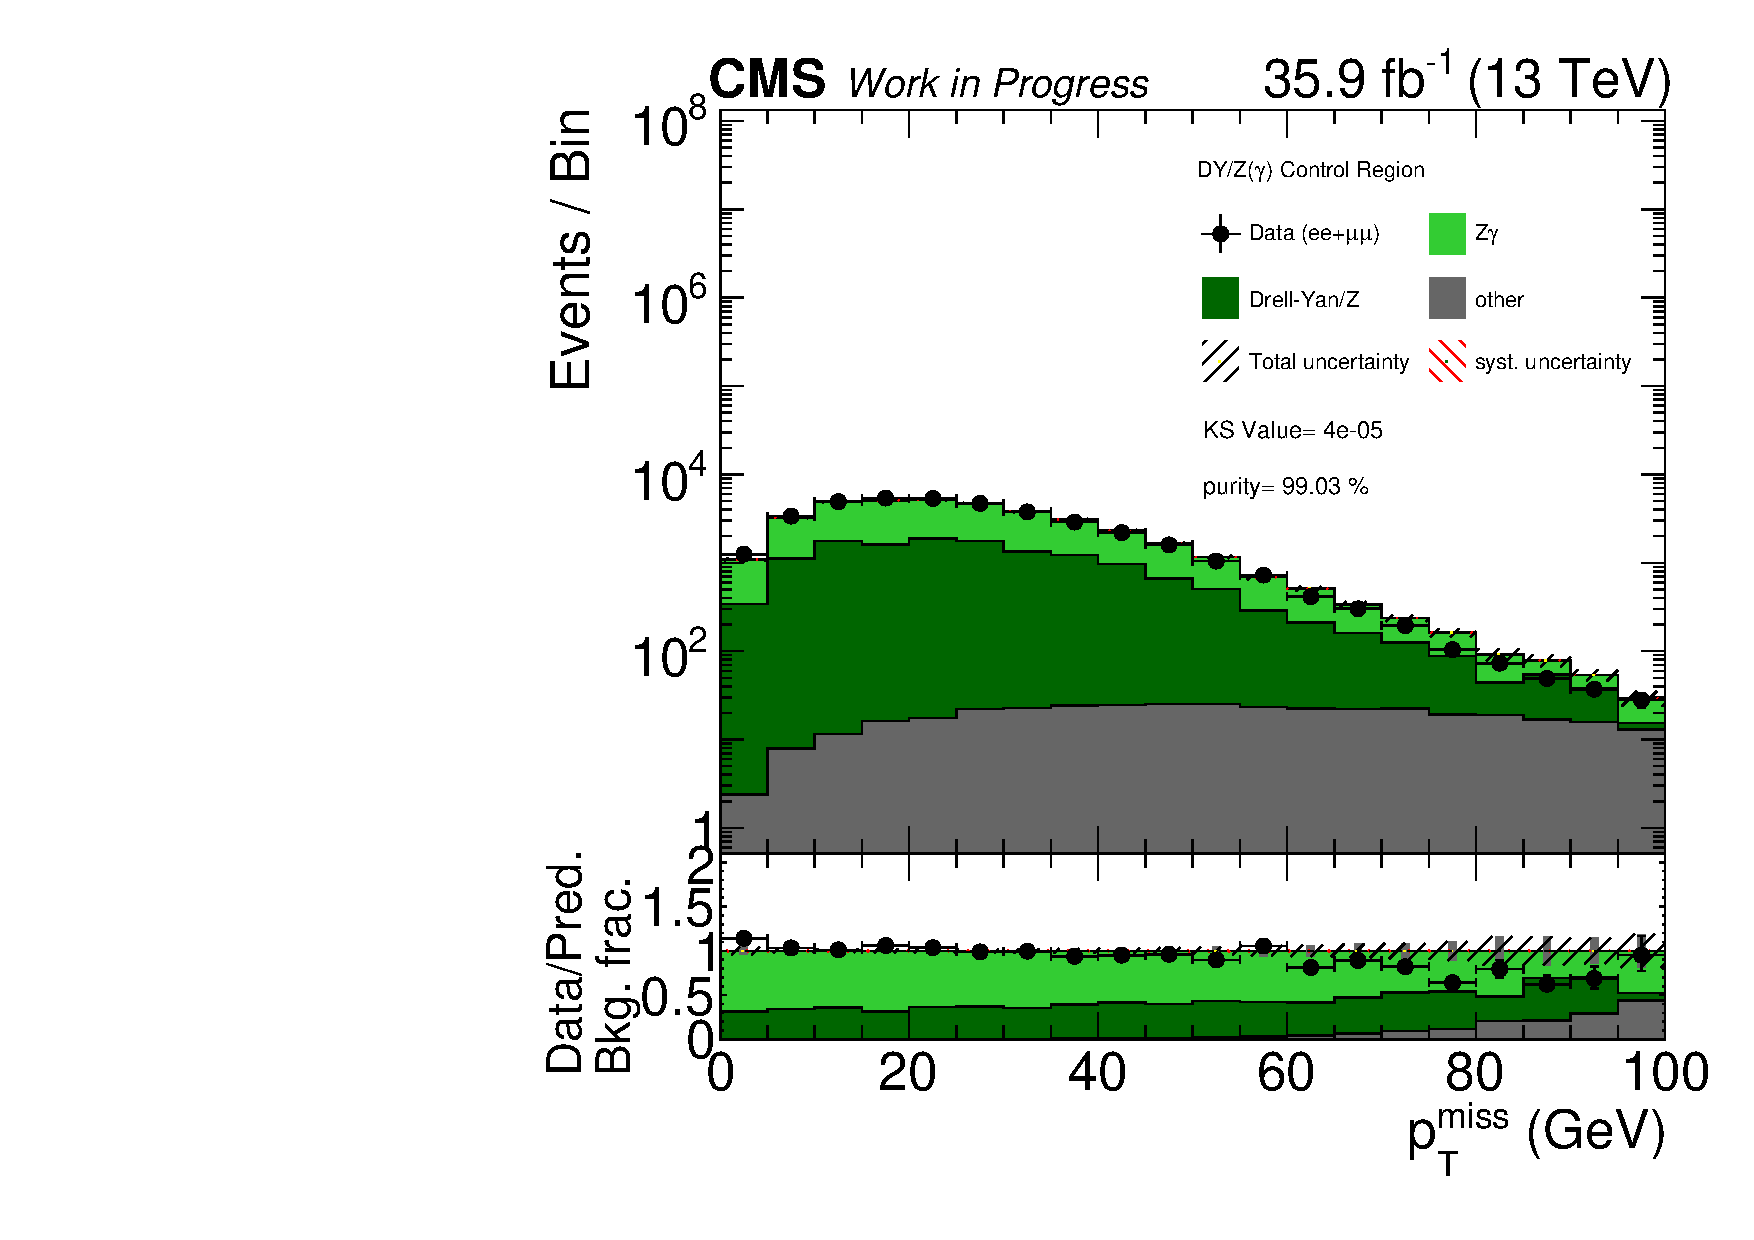
\includegraphics[width=\pairwidth]{figures/plots_CR_dy/CRDY_LL_nom_met_log}
 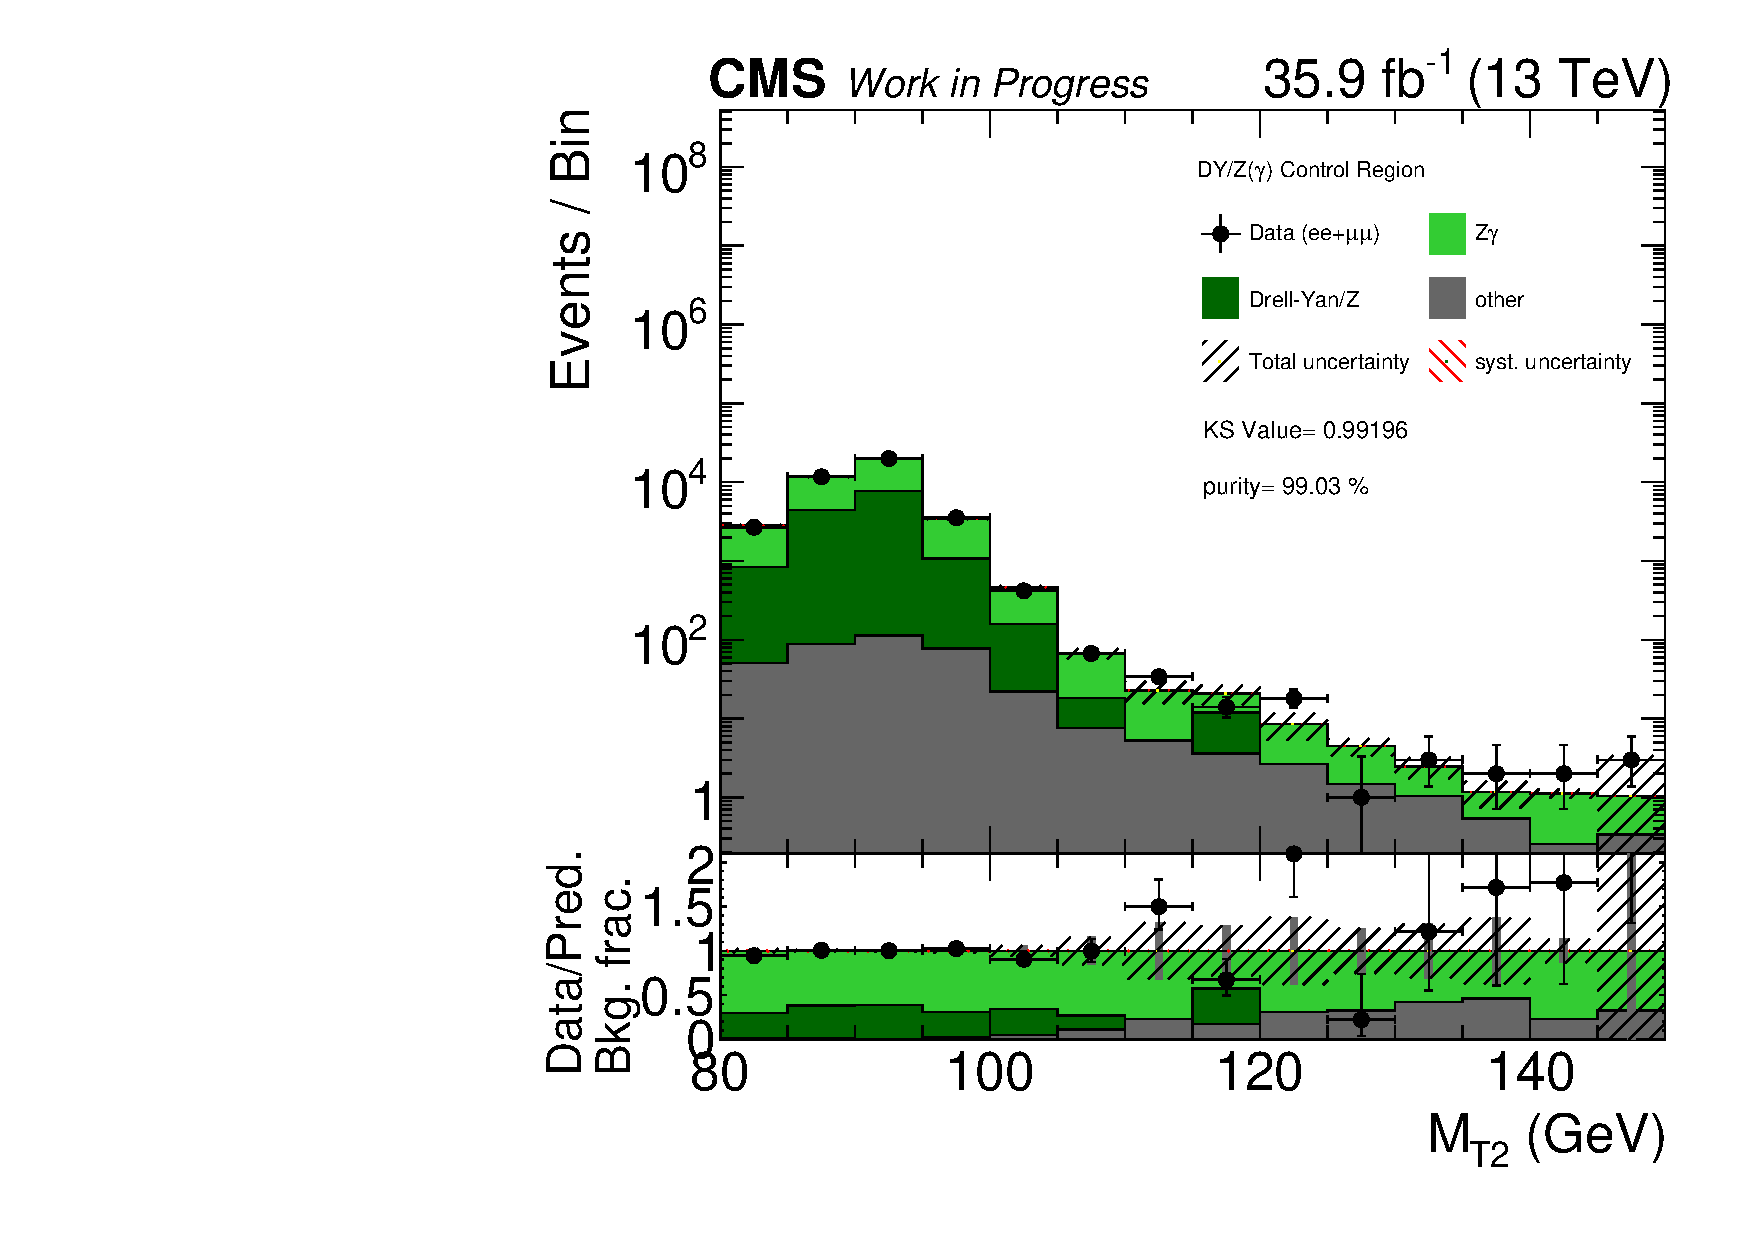
\includegraphics[width=\pairwidth]{figures/plots_CR_dy/CRDY_LL_nom_mt2_log}
 \caption{Comparisons between data and rescaled simulation in the DY/$\PZ(\PGg)$ CR in the $\ptmiss$ and $\mtTwo$ distribution. Below each plot, a ratio between data and prediction is shown. The uncertainty bands correspond to the systematic (red) and total uncertainty (gray). In addition, in the ratio plot the relative composition of the backgrounds is visualized. KS-values for the performed Kolmogorov-Smirnov test and the selection purity are also quoted.}
 \label{fig:CRDY}
\end{figure}
The $\chi^2$-fit studies, shown in \refFig{fig:chiDY} show good agreement over all variations.
% The $\chi^2$-fit studies, shown in \refFig{fig:chiDY} together with an example fit in the $\ptmiss$ distribution, show good agreement over all variations.

\begin{figure}[tbp]
 \centering
 % 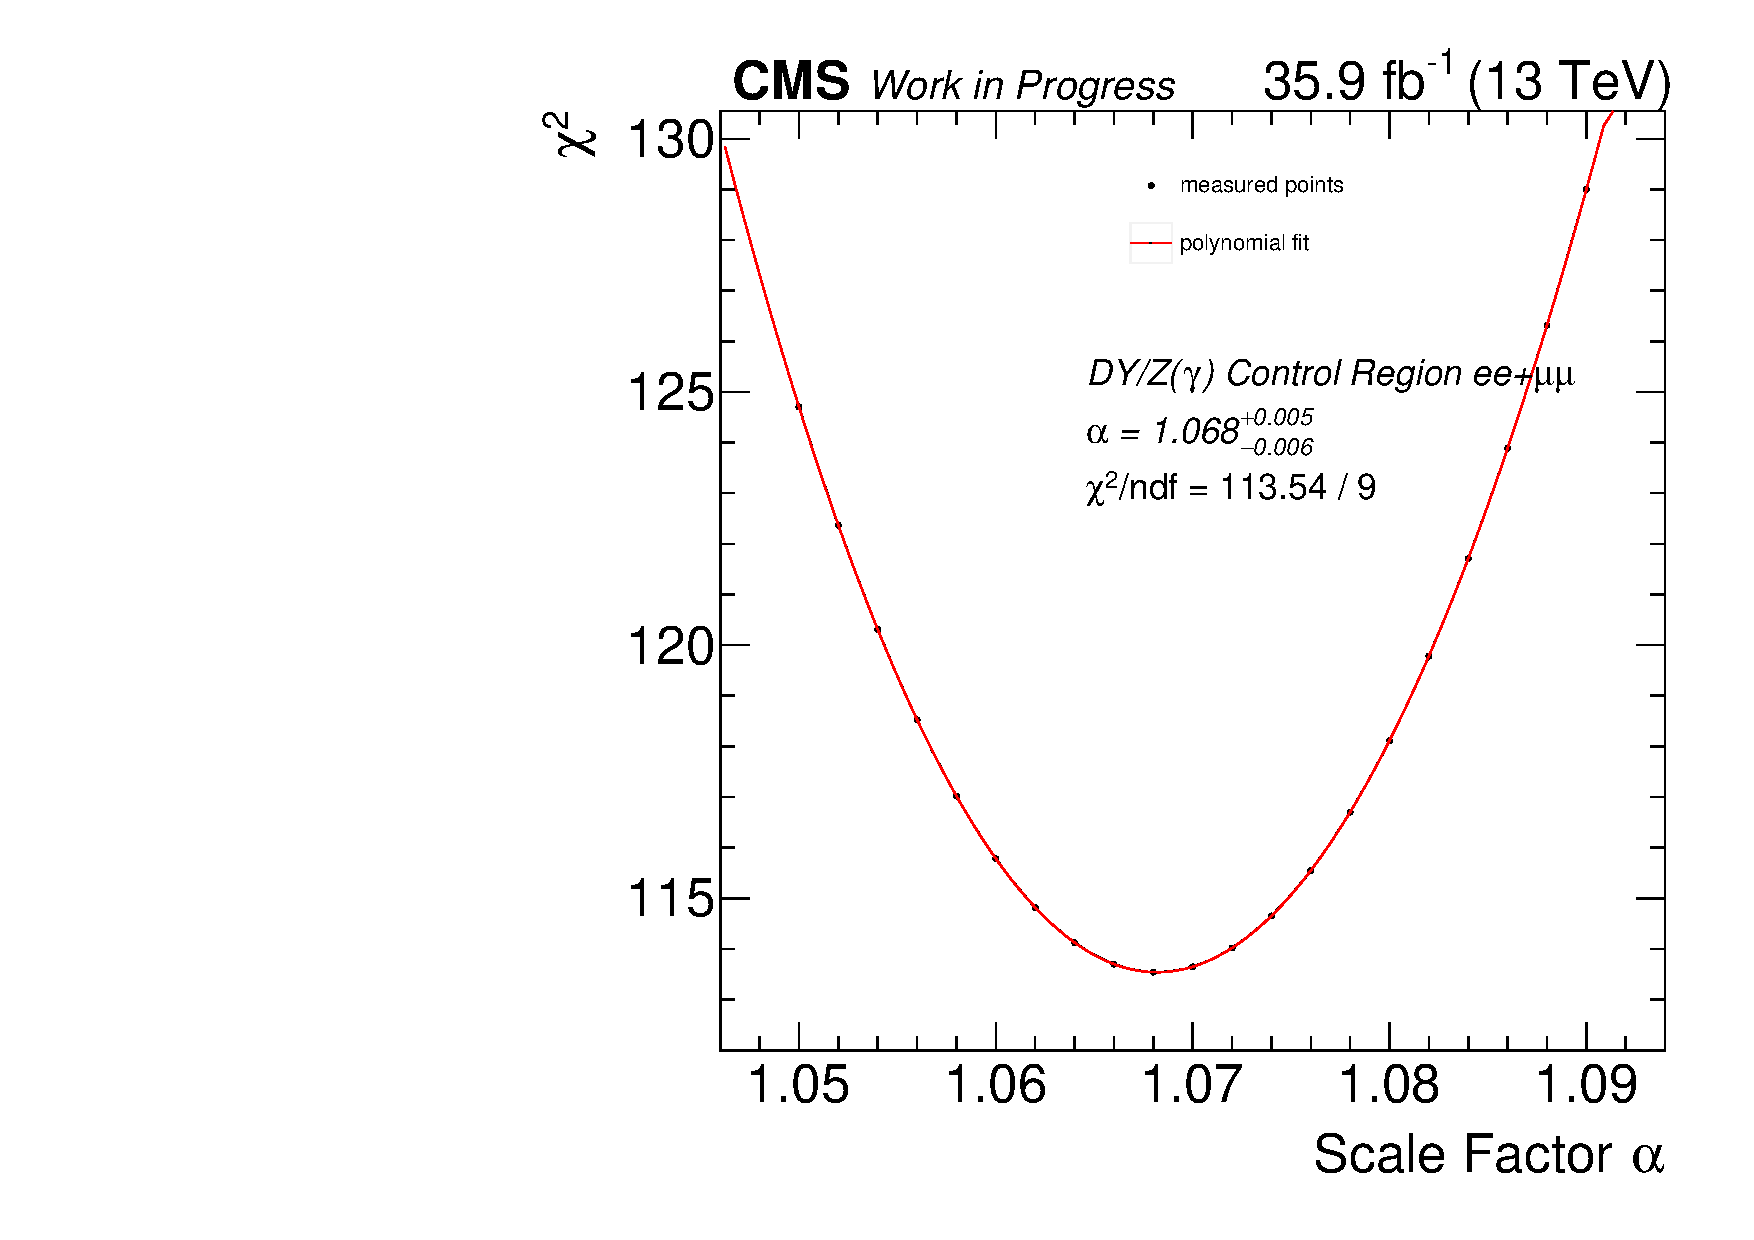
\includegraphics[width=\pairwidth]{figures/plots_CR/chi/DY_LL_met}
 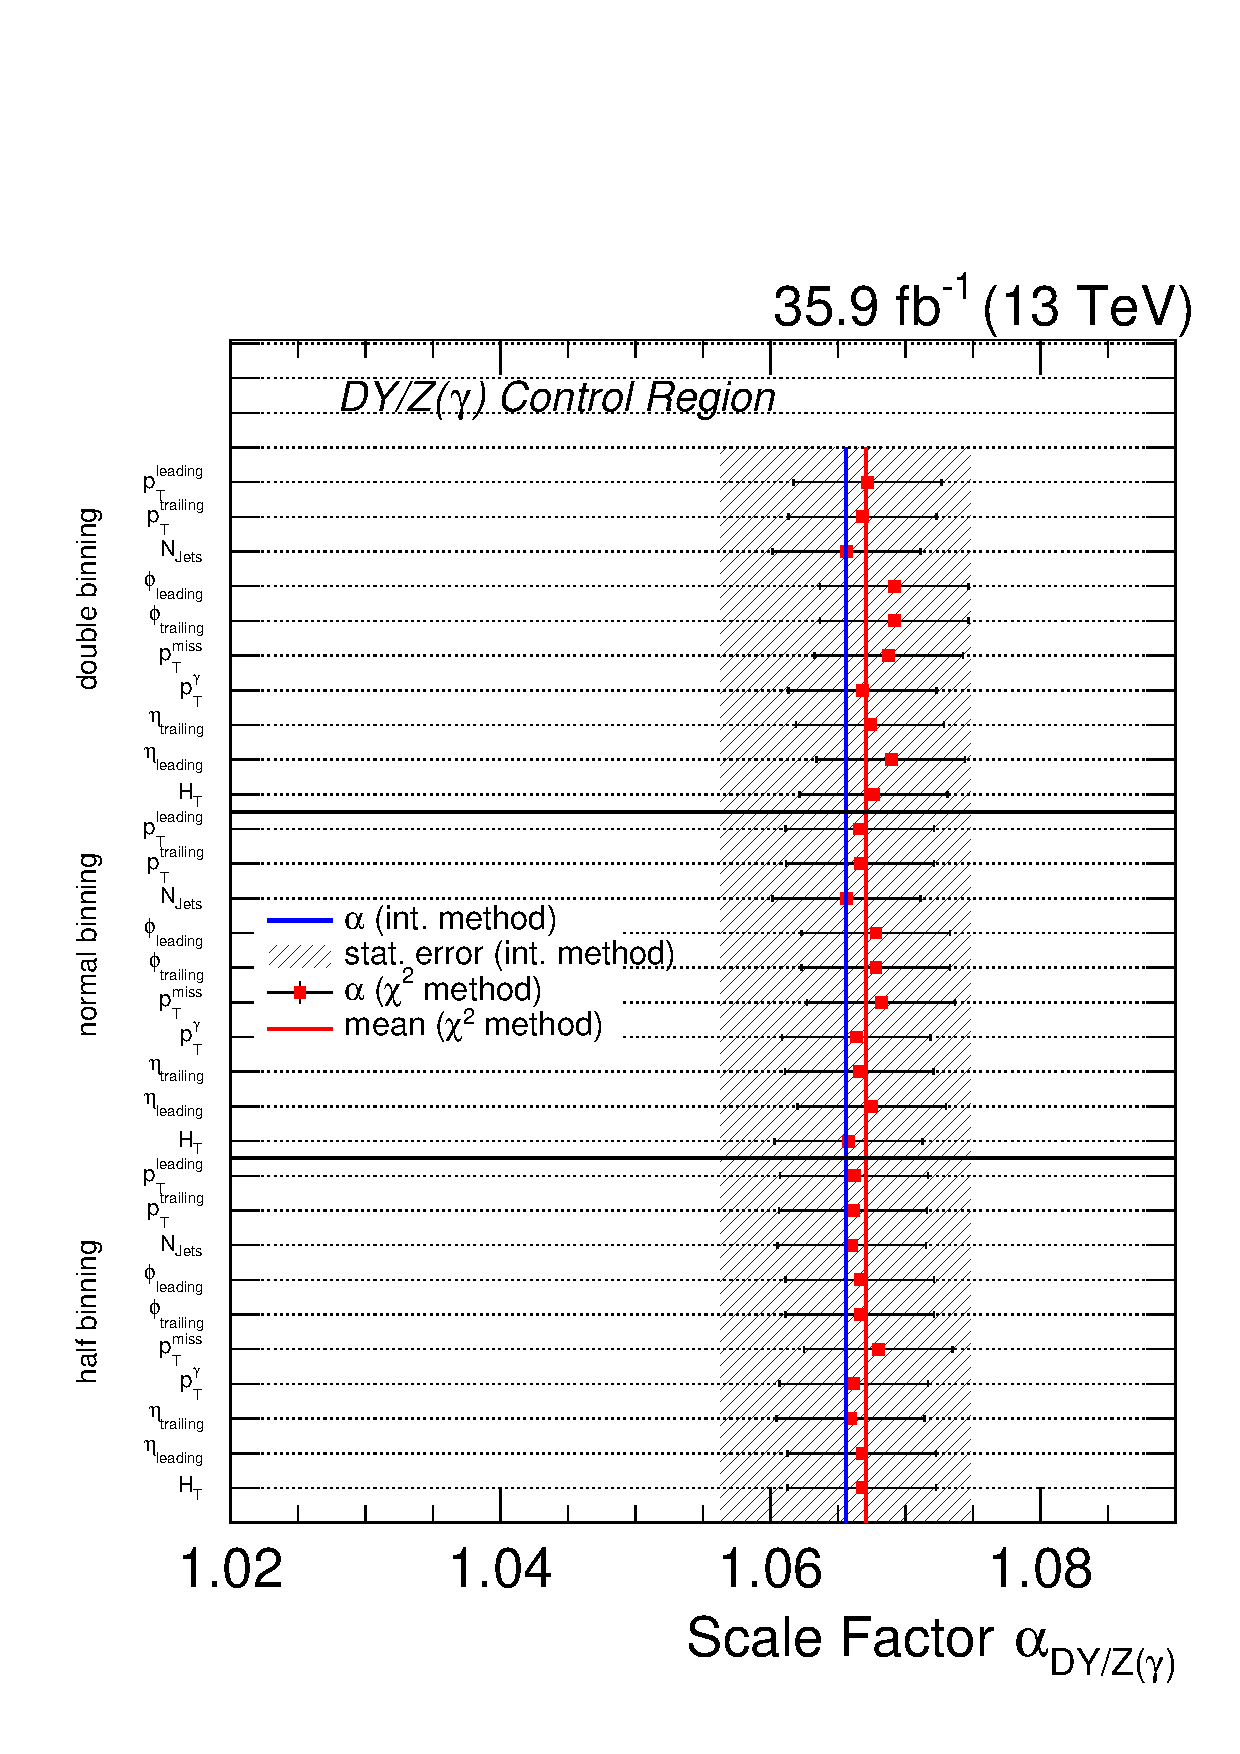
\includegraphics[width=\pairwidth]{figures/plots_CR/chi/DY_CompareLL}
 % \caption{Example $\chi^2$-fit in the DY/$\PZ(\PGg)$ CR in the $\ptmiss$ distribution (left) with the polynomial fit. All fit results compared with the SF obtained from the integral method in different binnings and variables (right).}
 \caption{All $\chi^2$-fit results compared with the SF obtained from the integral method in different binnings and variables.}
 \label{fig:chiDY}
\end{figure}



\subsection{Other standard model backgrounds}
Additional minor backgrounds, such as $\PW\PZ\PGg$, $\PW\PW\PGg$, $\PW\PW$, and $\PW\PGg$ production, the production of $\PW$ bosons in association with jets, and single top processes as listed in \refTab{tab:MCsamples}, are taken from plain simulation after reweighting them as described in \refSec{sec:Simulation} to the measured luminosity and NLO and NNLO cross sections.

\FloatBarrier
\subsection{Validation of the background estimation}\label{sec:Validation}
After all main backgrounds are estimated using the corresponding CRs where the SFs are determined, the background prediction is validated in the VR defined in \refSec{sec:VR}. The VR is orthogonal to the SR while being not signal sensitive and kinematically similiar to the SR. Therefore, the VR is ideal to study the obtained background prediction.\\
Resulting comparisons between prediction and observed data in different distributions are shown in \refFig{fig:VR1} for the most important variables, such as $\ptmiss$ and $\mtTwo$, together with $\pt$ distributions of the leading and trailing lepton. Comparisons for the photon $\pt$ and the invariant dilepton mass $m_{\ell\ell}$ distributions are shown in \refFig{fig:VR2}.\\
Overall, the agreement is good in all distributions, although being limited by the low statistics in some kinematic regions. The largest deviation is observable in the $\ptmiss$ distribution, but is consistent with the measured data within the statistical uncertainty in all bins. Statistical fluctuations of the DY/$\PZ(\PGg)$ backround are present, leading to such discrepancies. Although this background has an influence in the VR, its contribution in the SR is very small. Hence, the background prediction in the SR is not affected. In addition, Kolmogorov-Smirnov tests are performed to gain more trust in the background prediction. As can be read from the resulting KS-values, each quoted on the corresponding plot, the predicted and observed shapes agree well considering statistical uncertainties and systematic uncertainties, also in the $\ptmiss$ distribution. Here, the shown systematic uncertainty originates merely from the statistical ones from the integral method. With $97$ data events measured and $93.9$ predicted, als the total number of events match between prediction and data.\\
Therefore, the background are assumed to be well predicted in the SR due to the similar kinematics in the VR based on the design as a kinematic sideband in $\ptmiss$ and $\mtTwo$.
\begin{figure}[tbp]
 \centering
 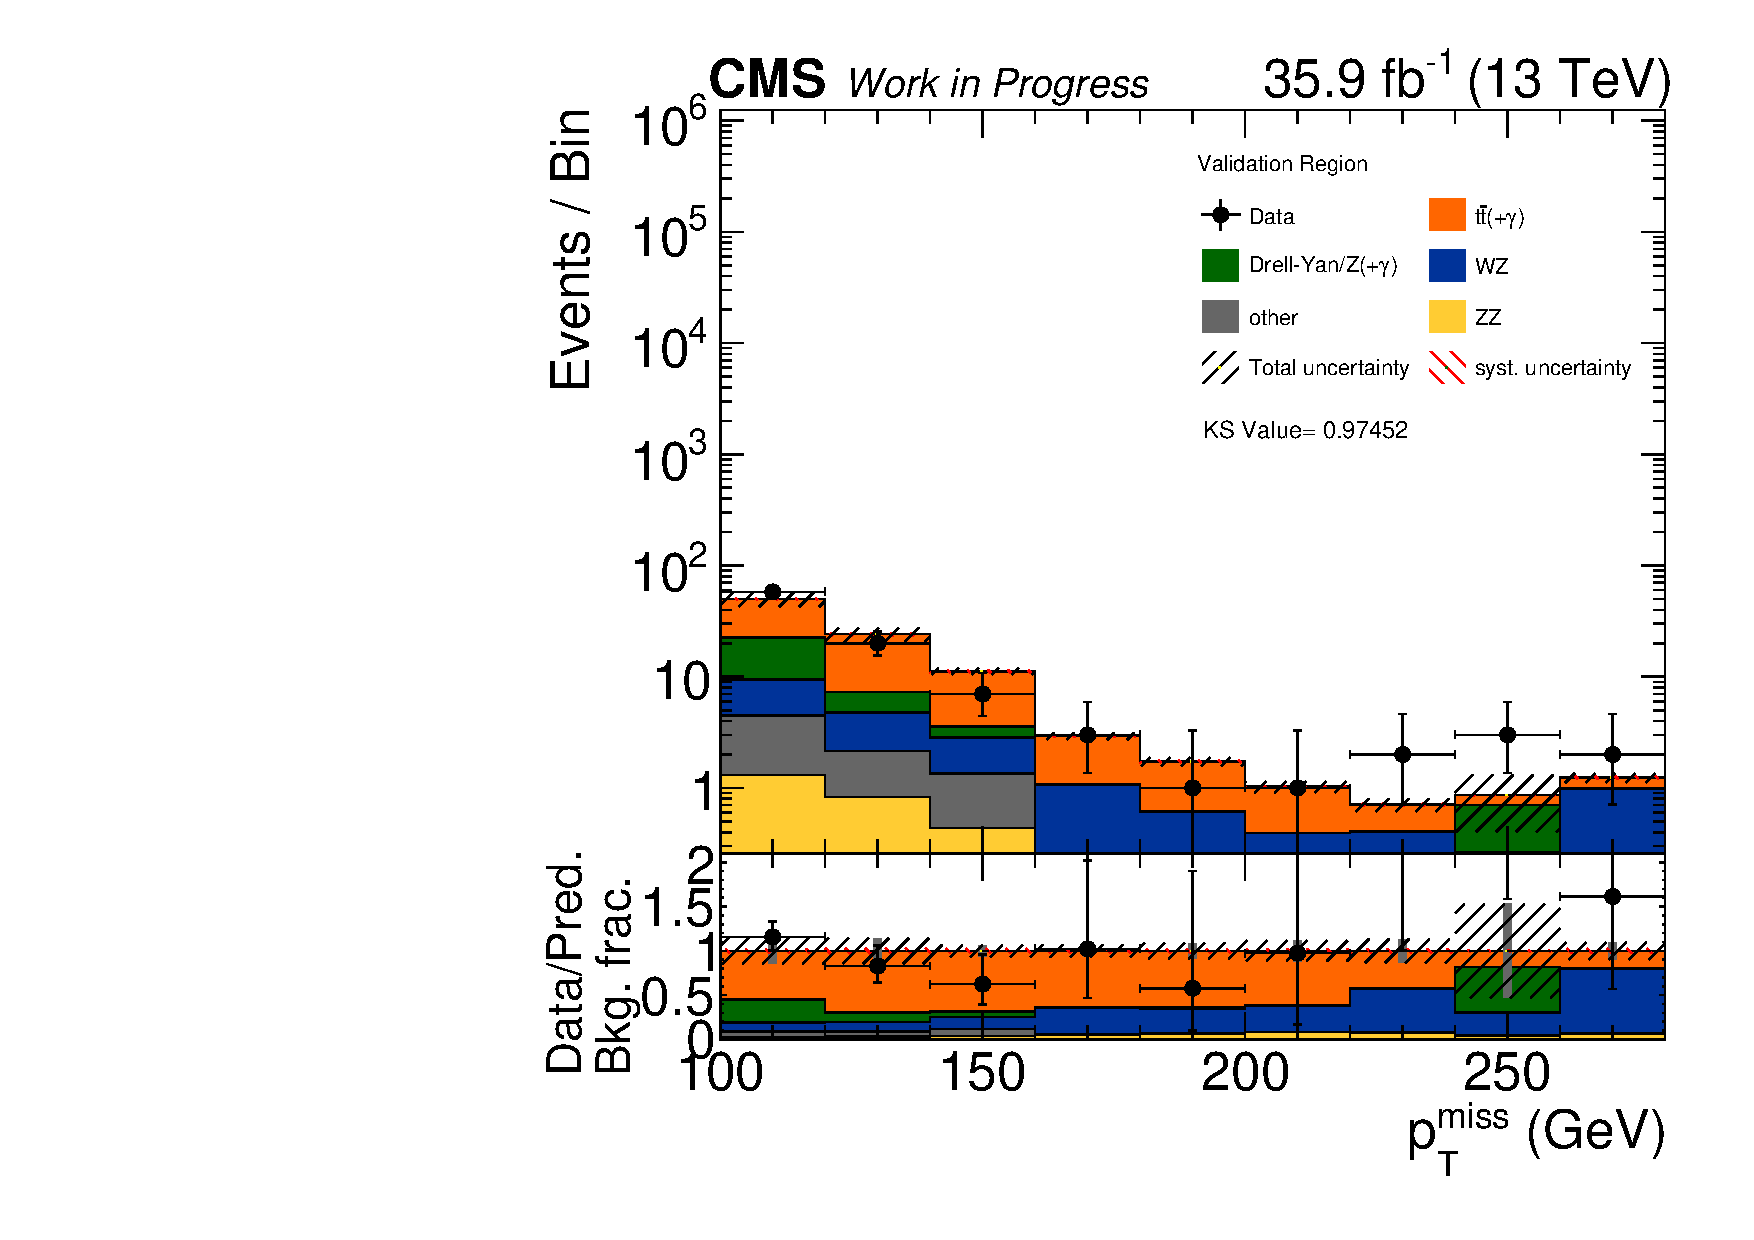
\includegraphics[width=\pairwidth]{figures/plots_VR/VR_LL_met_log}
 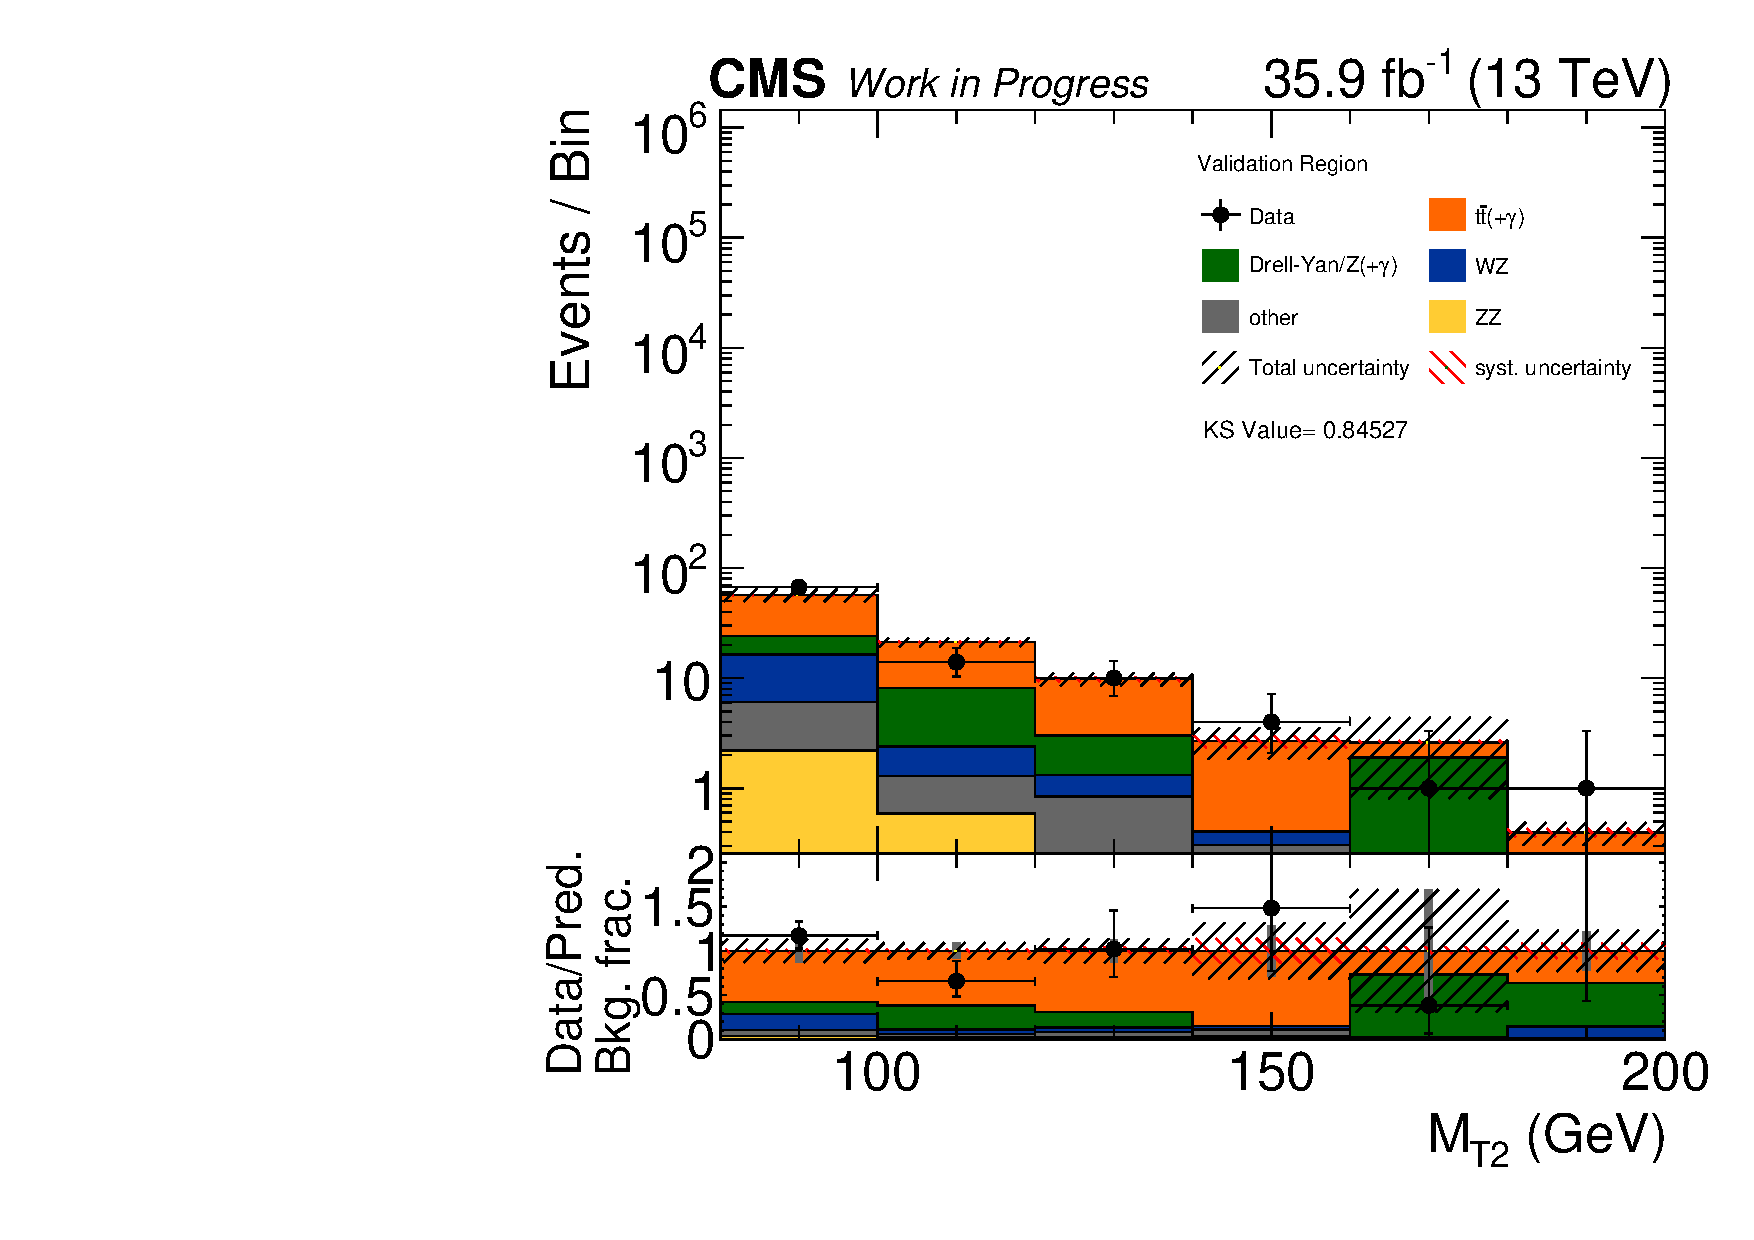
\includegraphics[width=\pairwidth]{figures/plots_VR/VR_LL_mt2_log}\\
 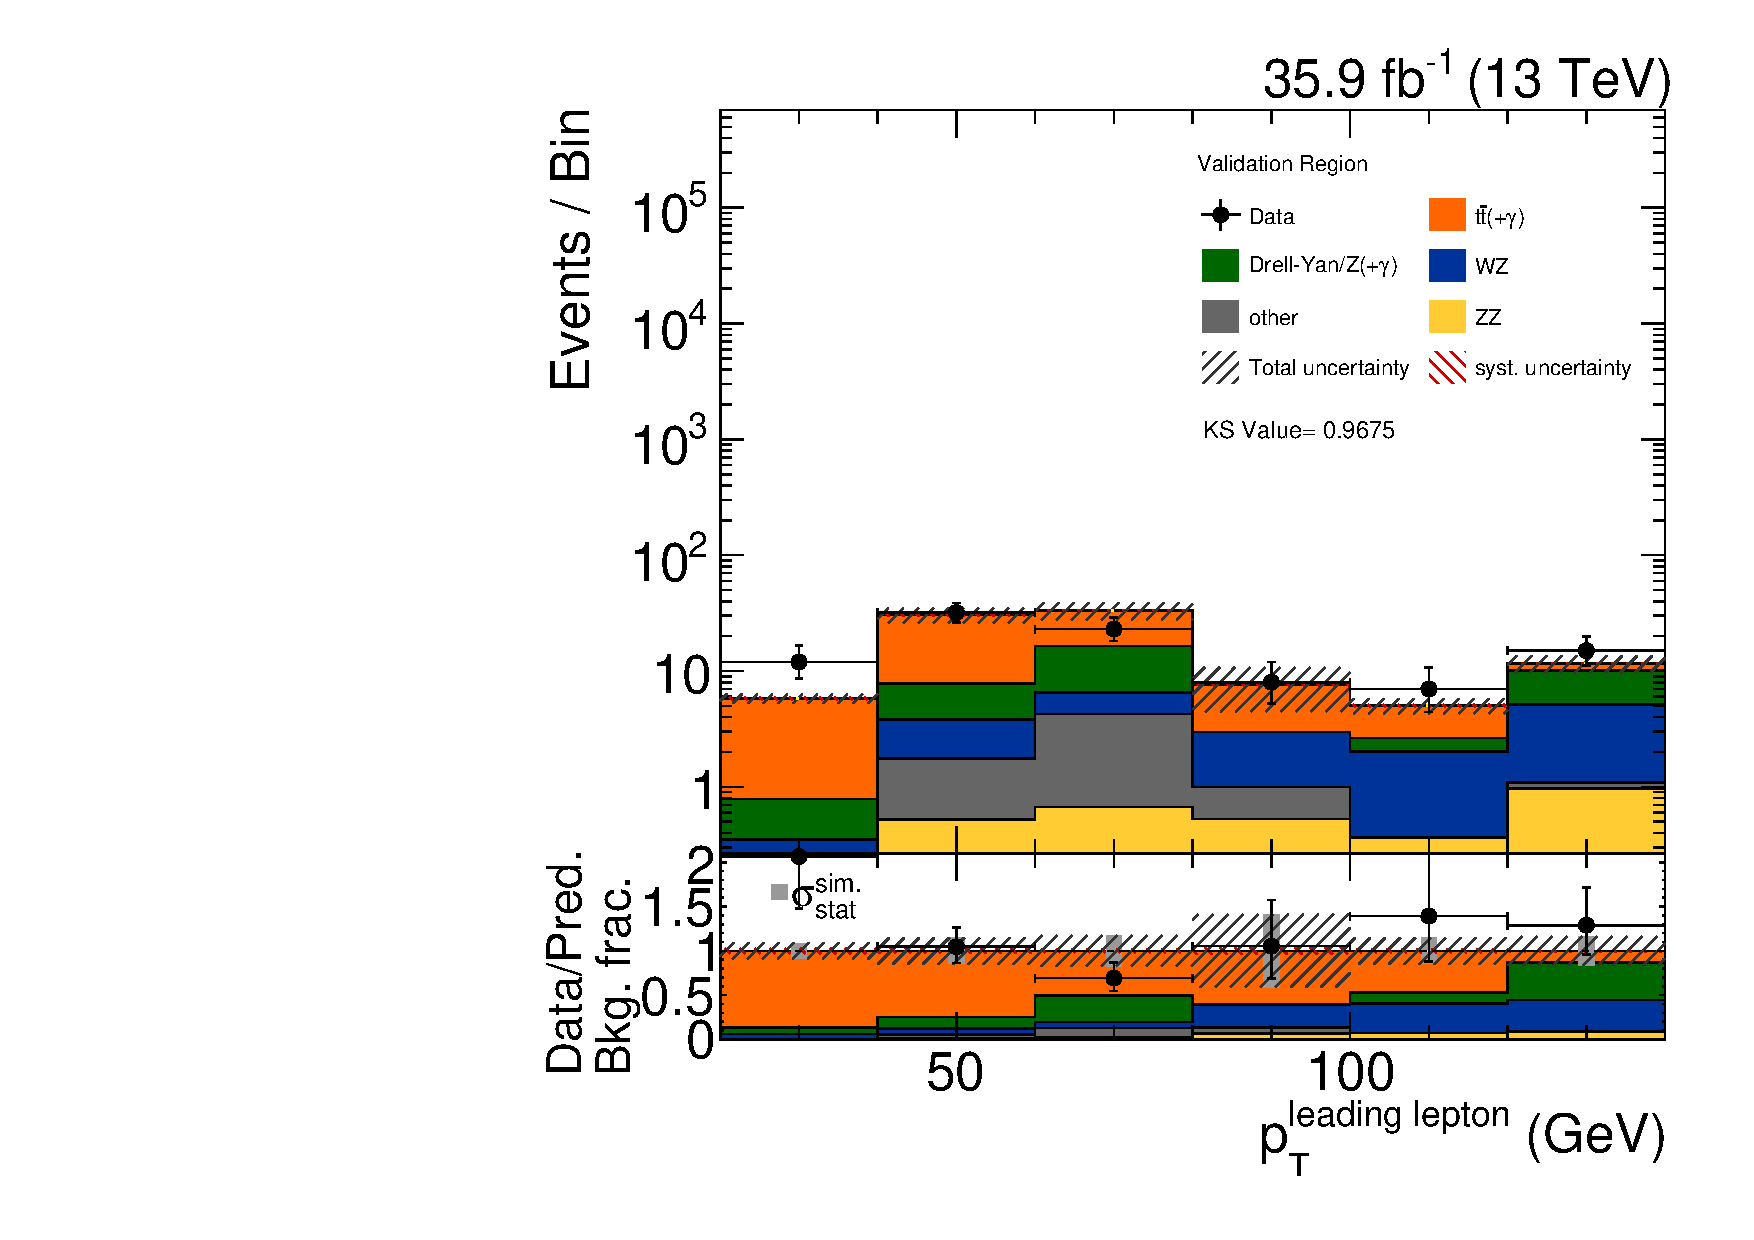
\includegraphics[width=\pairwidth]{figures/plots_VR/VR_LL_pt1_log}
 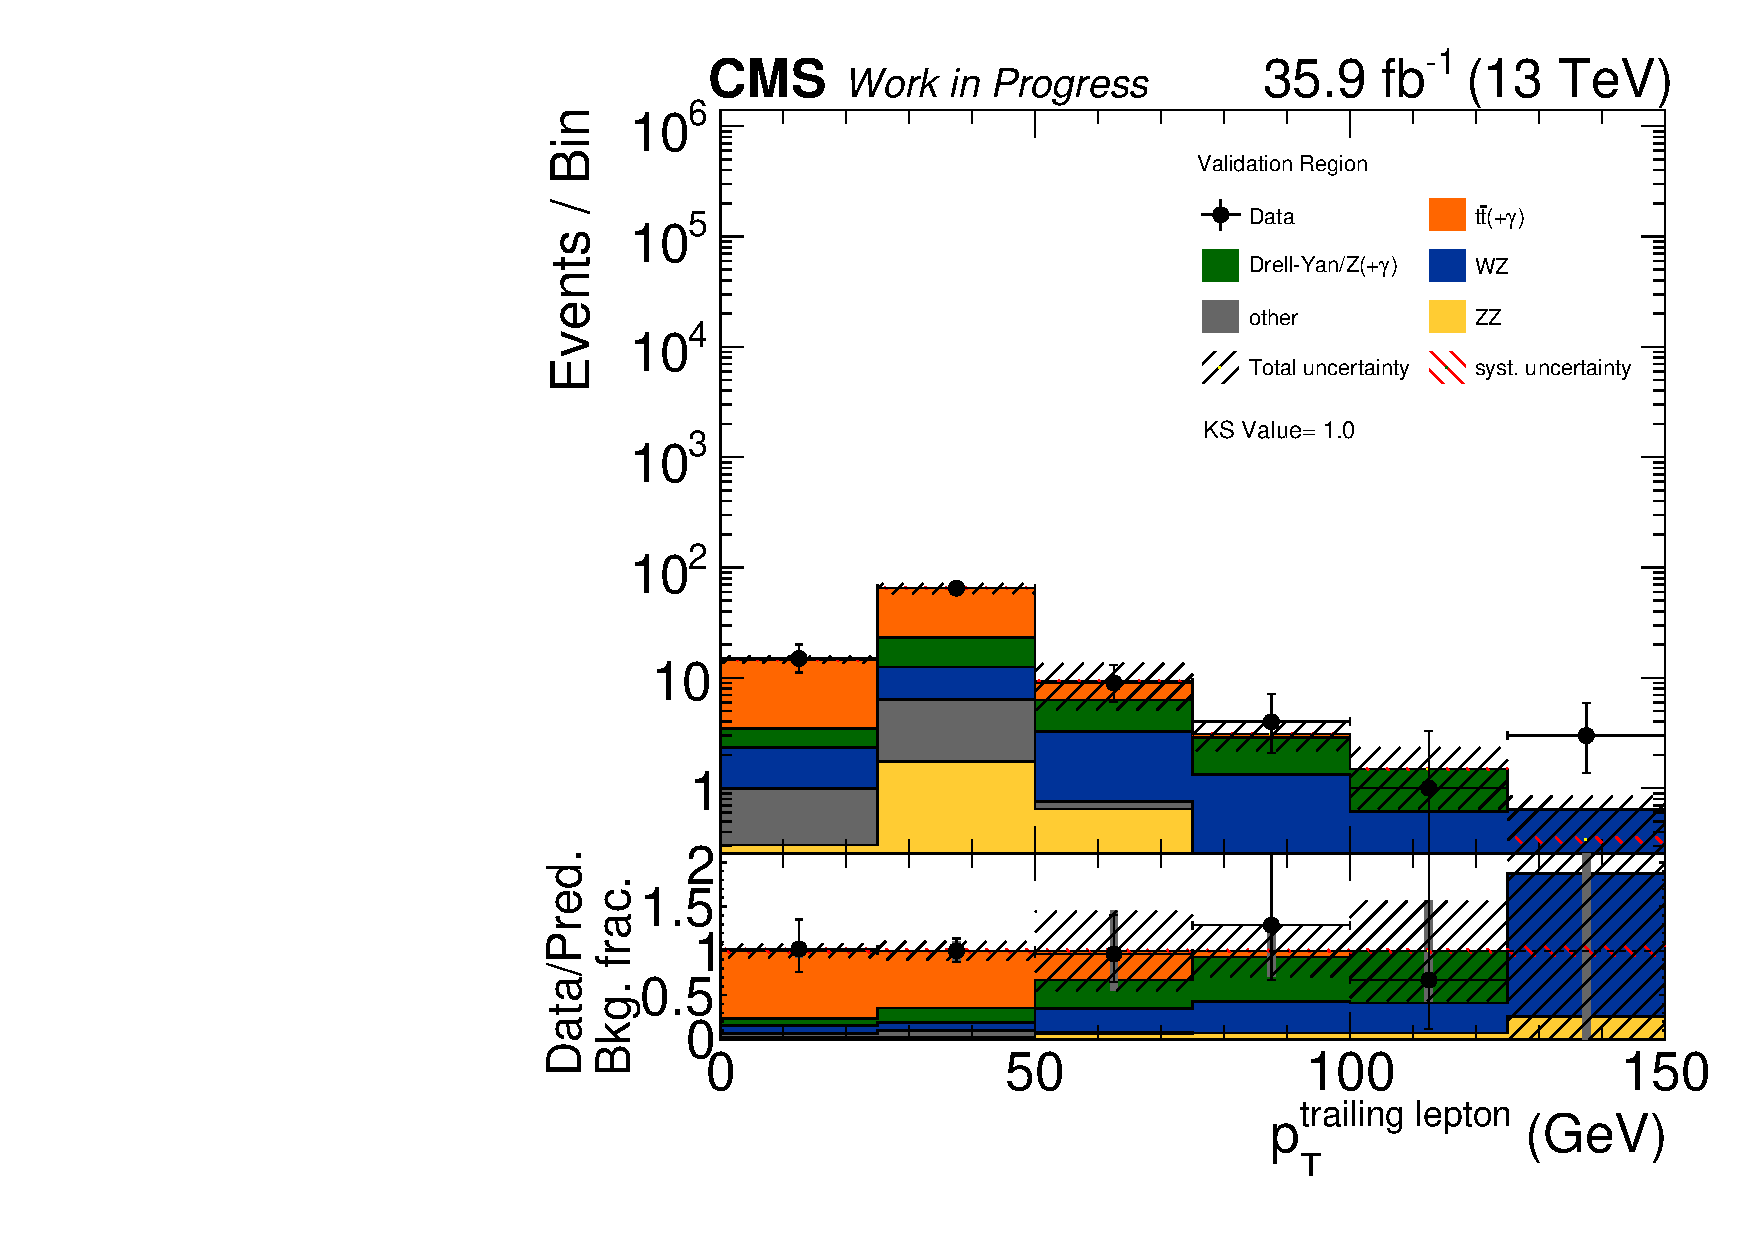
\includegraphics[width=\pairwidth]{figures/plots_VR/VR_LL_pt2_log}
 \caption{Comparisons between data and rescaled simulation in the VR in the $\ptmiss$, $\mtTwo$, and lepton $\pt$ distributions. Below each distribution, a ratio between data and prediction is shown. The uncertainty bands correspond to the systematic (red) and total uncertainty (gray). In addition, in the ratio plot the relative composition of the backgrounds is visualized. KS-values for the performed Kolmogorov-Smirnov test and the selection purity are also quoted.}
 \label{fig:VR1}
\end{figure}


\begin{figure}[tbp]
 \centering
 \includegraphics[width=\pairwidth]{figures/plots_VR/VR_LL_pt_g1_log}
 \includegraphics[width=\pairwidth]{figures/plots_VR/VR_LL_m_ll_log}
 \caption{Comparisons between data and rescaled simulation in the VR in the photon $\pt$ and invariant dilepton mass distribution. Below each distribution, a ratio between data and prediction is shown. The uncertainty bands correspond to the systematic (red) and total uncertainty (gray). In addition, in the ratio plot the relative composition of the backgrounds is visualized. KS-values for the performed Kolmogorov-Smirnov test are also quoted.}
 \label{fig:VR2}
\end{figure}


\subsection{Signal contamination}\label{sec:signalCont}
If SUSY was realized in nature, it would not only produce events in the SR, but also some of them may appear in the CRs that are used to determine a proper background prediction. To account for this effect, the so-called signal contamination of the background CRs is not considered in the background estimation itself, but is translated into a reduction of the predicted signal yield in the SR. Hence, the signal contamination needs to be measured for each signal point of all samples individually in all CRs.\\
Therefore, the fraction of expected signal events relative to the total number of background events in each CR is measured.
Examplary, the signal contamination for GMSB model in the DY/$\PZ(\PGg)$ CR and $\PW\PZ$ CR are shown in \refFig{fig:signalCont}, because they are the largest ones observed due to the variety of decay topologies in this model. As can be seen, the contributions of signal events are mainly negligible, although the signal contamination reaches around $3\%$ for very low bino and wino masses.\\
% Examplary, the contamination of the \texttt{TChiZG} SMS in the DY/$\PZ(\PGg)$ CR and the GMSB model in the $\PW\PZ$ CR are shown in \refFig{fig:signalCont}, because they are the largest ones observed. As can be seen, the contributions of signal events are mainly negligible, although the signal contamination reaches around $3\%$ for very low bino and wino masses in the GMSB model.\\
To account for those effects, these relative fractions are used to lower the signal expectation in each SR bin individually. If $\rho$ is the fraction of signal events in the CR, in each SR bin the absolute signal event yield reduced with the following formula
\begin{equation}
 \#signal_{after} = \#signal_{before} - \rho\cdot\#background,
\end{equation}
where $\#signal_{before}$ and $\#signal_{after}$ are the total number of signal events per bin before and after the correction, and $\#background$ is the number of predicted background events in this bin.

\begin{figure}
 % \includegraphics[width=\pairwidth]{figures/contamination/tching_DY}
 \includegraphics[width=\pairwidth]{figures/contamination/gmsb_tt}
 \includegraphics[width=\pairwidth]{figures/contamination/gmsb_WZ}
 \caption{Signal fraction compared to the total background event yield for different signal points of the \texttt{TChiZG} in the DY/$\PZ(\PGg)$ CR (left) and the GMSB model in the $\PW\PZ$ CR (right).}
 \label{fig:signalCont}
\end{figure}
In total, the influence of signal contamination to the final result is rather negligible, because for most of the signal points the contributions to all CRs are very low. In cases where they exceed the level of a few percent, their influence will not matter in the final interpretation, since for those low SUSY mass signal points, the expectation for the signal yield in the SR is sufficiently high.


\section{Study of systematic uncertainties}\label{sec:Syst}
In addition to the statistical uncertainties arising from the background prediction method itself, various systematic effects and their impact on the final prediction need to be evaluated.

\subsection{Background uncertainties}
Systematic uncertainties arise from the data pileup distribution, which is used to rescale the simulated samples as explained in \refSec{sec:Simulation}, the measurement of the total integrated luminosity, the measurement of the jet energy scale (JES) and the jet energy resolution (JER), the measured trigger efficiencies as discussed in \refSec{sec:triggEff}, corrections for a different photon and lepton reconstruction efficiency in simulation and data, the PDF sets used in the simulation process, and choice of the factorization scale and renormalization scale.\\
These measurements and underlying effects all contribute systematic uncertainties on the final background prediction. Cross section, trigger, and luminosity uncertainties cancel for the four main background contributions due to the integral method, but are relevant for the other minor contributions. For these a cross section uncertainty of $50\%$ is assigned to the final yield to account for differences between cross section measurement and theoretical prediction, and to consider the circumstance, that only a special phase space region is investitaged in the analysis.\\
The uncertainty on the luminosity measurement with $2.5\%$~\cite{LumiUncert} and the uncertainty on the trigger efficiency, that is estimated to be $3\%$ (see \refSec{sec:triggEff}), propagate directly to the final prediction.\\
All other uncertainties are uncertainties in the shapes of the predicted spectra, and need to be determined in another way. In order to estimate the impact of the JES and JER, the pileup reweighting, and the lepton and photon identification and reconstruction corrections, the background prediction is performed again with the underlying quantities shifted one standard deviation up and down. Hence, two additional predictions for each SR bin are obtained, and half of the difference between those, relative to the nominal prediction, is taken as the corresponding systematic uncertainty.\\
The uncertainty arising from the JES (JER) is observed to be around $1-6.5\%$ ($0.2-16.1\%$) for the four main backgrounds, while uncertainty arising from the lepton (photon) identification and reconstruction is $1.8-3.2$ ($0.7-1.5\%$). The uncertainty due to pileup reweighting varies between $0.2\%$ and $5\%$ for these four backgrounds. For the other backgrounds the uncertainties are higher, but the absolute effect is negligible compared to the other background controbutions due to the low predicted event yields.
To estimate the effect on the choice of the renormalization scale $\mu_R$ and factorization scale $\mu_F$, these two are varied in combinations of the factors $0.5$, $1$, and $2$, and eight new background predictions are obtained. The half of the difference between the two outliers, relative to the nominal prediction, is chosen as the systematic uncertainty. It varies between $21.-22.5\%$ for all backgrounds over all bins.\\
To determine the systematic uncertainty arising from the used PDF sets, one hundred different PDF variations are studied, and for each the background prediction method is performed again, thus one hundred different predictions for the SR are obtained. From this distribution of predicted yields, the standard deviation and the mean can be calculated. The standard deviation with respect to the mean is considered as the systematic uncertainty, and varies between $0.8\%$ and $3.3\%$ for all backgrounds and bins.\\
The uncertainty arising from the choice of order regarding the four SFs determined in the CRs, is estimated by testing all $4!=24$ possibilities, and calculating the largest deviation from the nominal SFs. This envelope is considered as a systematic uncertainty on the SFs on top of the statistical uncertainty. Both uncertainties are added quadratically, such that one final uncertainty for each SF is obtained.
\refTab{tab:systuncBKG} lists ranges for all final systematic uncertainties for all backgrounds individually.
\begin{table}[tbp]
 \centering
 \caption{Systematic uncertainty ranges for all background predictions in the signal region.}
 \small
 \label{tab:systuncBKG}
 \begin{tabular}[width=\textwidth]{llllll}
                            & $tt(\PGg)$  & DY/Z$(\PGg)$  & $\PW\PZ$    & $\PZ\PZ$    & Other       \\\hline
  PDF                       & $0.8-1.5\%$ & $2.6-3.3\%$   & $0.5-0.7\%$ & $2.2-2.4\%$ & $1.1-1.2\%$ \\
  Renorm. and fact. scale   & $3.3-7.1\%$ & $18.2-22.5\%$ & $4-6\%$     & $3.7-4.1\%$ & $2.1-9.3\%$ \\
  Jet energy scale          & $4.6-6.5\%$ & $4.4-5\%$     & $2.8-4.8\%$ & $1-1.9\%$   & $0-50.7\%$  \\
  Jet energy resolution     & $1.6-3.1\%$ & $0.7-16.1\%$  & $1-1.8\%$   & $0.2-1.4\%$ & $0-50.7\%$  \\
  Lepton ID and reco.       & $2.8-2.9\%$ & $2.2-3.4\%$   & $3.3\%$     & $1.8\%$     & $4.2\%$     \\
  Photon ID and reco.       & $0.7-0.8\%$ & $1.4-1.5\%$   & $1-1.1\%$   & $0.9\%$     & $0.7-1.9\%$ \\
  Luminosity                & -           & -             & -           & -           & $2.5\%$     \\
  Pileup                    & $1.2-2\%$   & $1-5\%$       & $0.2-2.5\%$ & $1.5-1.7\%$ & $0.1-10\%$  \\
  Trigger efficiency        & -           & -             & -           & -           & $3\%$       \\
  Scale factor $\alpha_{i}$ & $4.1\%$     & $0.9\%$       & $3.9\%$     & $5.7\%$     & -           \\
  Cross section             & -           & -             & -           & -           & $50\%$      \\
  \hline
 \end{tabular}
 \vspace{\baselineskip}
\end{table}
Besides uncertainties for some backgrounds, such as DY/$\PZ(\PGg)$ and the other composed backgrounds, exceed the level of $10\%$, where statistical fluctuations based on changes of different quantities play an important role, all other systematic uncertainties are of the order of a few percent. This reflects the stability and robustness, that was observed in the scale factor determination itself.


\subsection{Signal uncertainties}
Signal uncertainties need to be studied in order to interpret the results statistically in each SUSY model.
Most of the signal uncertainty determination methods behave the same as for the backgrounds, but some additional effects need to be considered. Some calculations change, since the detector response in the signal MC simulation was performed using the \FASTSIM package.\\
For the determination of the pileup uncertainty, a different method is applied. The pileup distribution is split into a low PU ($N_{vertices}<20$) and a high PU ($N_{vertices}>20$) region, and the difference in the total signal acceptance is determined. Half of this difference is treated as the systematic uncertainty.\\
Because the modeling of the $\ptmiss$ distribution is very complicated, and in the \FASTSIM package only a simplified detector response is parameterized, the difference between generated $\ptmiss$ and reconstructed $\ptmiss$ is investigated. Thus, the whole analysis is reperformed for the signal, where the reconstructed $\ptmiss$ is replaced with the generated $\ptmiss$ for each event, and the difference in the acceptance is examined. Half of the deviation is taken as the systematic uncertainty.\\
For the signal simulation, no PDF uncertainties are available. The initial state radiation dependent reweightings mentioned in \refSec{sec:Simulation} introduce systematic effects on the signal yield expectation. Therefore, the same method as mentioned above for the identification and reconstruction uncertainties on the background prediction is performed.\\
Ranges for all signal uncertainties including the statistical one are given in \refTab{tab:systuncSignal} altogether for all signal models considered in the analysis split into electroweak and strong production scenarios.\\
All other systematic effects, except for the luminosity uncertainty and the uncertainty arising from the trigger efficiency measurement are correlated with the statistical uncertainty.
Hence, large ranges are observable due to the limited statistics that is available for each signal point. This is due to time and resource saving reasons, since a large number of different signal points is being generated. In addition, the low available number of signal events becomes much lower, as only leptonic decay branches of the Z boson are considered and its branching fraction ($\mathcal{BR}(\PZ\to\ell^+\ell^-)\approx3.36\%$~\cite{PDG}) is very low. Nevertheless, in most of the relevant signal points the uncertainties do not exceed the level of a few percent.
\begin{table}[tbp]
 \centering
 \caption{Ranges for all the systematic uncertainties for all signal models.}
 \normalsize
 \label{tab:systuncSignal}
 \begin{tabular}[width=\textwidth]{lrr}
                                & \multicolumn{2}{c}{Range $[\%]$}                     \\
  Uncertainty                   & Electroweak production           & Strong production \\\hline
  Statistical                   & $3.9-71$                         & $2.5-100$         \\
  Luminosity                    & $2.6$                            & $2.6$             \\
  Pileup                        & $<0.1-93$                        & $<0.1-193$        \\
  Jet energy scale              & $<0.1-32$                        & $<0.1-62$         \\
  Jet energy resolution         & $<0.1-26$                        & $<0.1-64$         \\
  Trigger Efficiency            & $3$                              & $3$               \\
  Lepton ID and reconstruction  & $<1-5.6$                         & $0.8-2.1$         \\
  Photon ID and reconstruction  & $1.4-1.5$                        & $1.4-1.5$         \\
  \FASTSIM uncert. in $\ptmiss$ & $<0.1-97$                        & $<0.1-294$        \\
  ISR reweighting               & $2.6-3.9$                        & $5.9-11$          \\
  Renorm. and fact. scale       & $<0.1-1.6$                       & $<0.1-11$         \\
  \hline
 \end{tabular}
 \vspace{\baselineskip}
\end{table}
% \begin{table}[tbp]
%  \centering
%  \caption{Ranges for all the systematic uncertainties for all signal models.}
%  \normalsize
%  \label{tab:systuncSignal}
%  \begin{tabular}[width=\textwidth]{ll}
%   Uncertainty                   & Range $[\%]$ \\\hline
%   Statistical                   & $3.2-85$     \\
%   Luminosity                    & $2.6$        \\
%   Pileup                        & $<0.1-143$   \\
%   Jet energy scale              & $<0.1-62$    \\
%   Jet energy resolution         & $<0.1-63$    \\
%   Trigger Efficiency            & $3$          \\
%   Lepton ID and reconstruction  & $<0.1-5.6$   \\
%   Photon ID and reconstruction  & $1.4-1.5$    \\
%   \FASTSIM uncert. in $\ptmiss$ & $<0.1-293$   \\
%   ISR reweighting               & $<0.1-11$    \\
%   Renorm. and fact. scale       & $0.1-11$     \\
%   \hline
%  \end{tabular}
% \end{table}

\chapter{Results and interpretation}\label{chap:results}
\minitoc
Now that all backgrounds are well estimated, the background prediction is reliable in the validation region, and all uncertainties are determined, the background prediction methods can be applied to the SR, $\ptmiss>150\GeV$ and $\mtTwo>100\GeV$, and predicted and observed event counts can be compared. An excess of events or other significant deviations from the prediction could be indicators for BSM physics.
\section{Results}\label{sec:results}
\subsection*{Signal region binning}
In order to perform the counting experiment, a distinct binning in one or multiple variables needs to be applied to the SR. This binning can be optimized considering different criteria, \eg, observation and exclusion power. Since the most sensitive variables are $\ptmiss$ and $\mtTwo$, different one dimensional and two dimensional binnings are possible.
% For signal benchmark points of all three signal models, simplified significances $\frac{s}{\sqrt{s+b}}$, where s is the number of signal events and b the number of background events per bin, the binnings are varied.
Because the total predicted event count in the SR is approximately $13$ events, special care has to be taken regarding this low data yield. Albeit many sensitive bins with lower SM prediction and high signal expectation would push expected exclusion limits, this would make reinterpretations and observations difficult due to the high statistical uncertainties of the measured data. Considering that the $\ptmiss$ and $\mtTwo$ distributions are exponentially decreasing for the predicted backgrounds, the maximum number of bins is limited. Therefore, a binning consisting of two bins is chosen. It consists of two bins in the $\ptmiss$ distribution, as already introduced in \refSec{sec:SRSelection}. The first bin starts at $150\GeV$ and ends at $200\GeV$, while the second one gathers all events with $\ptmiss>200\GeV$ in the SR. This choice yields good exclusion power while containing a sufficient number of events in each bin, so that the reinterpretation is not restricted by statistical uncertainties. For the same reasons, higher dimensional binnings are discarded, too. The $\ptmiss$ distribution is preferred over the $\mtTwo$ distribution, because it is more model independent given the many decay possibilities in full theoretical models. In the calculation of $\mtTwo$, both bosons are assumed to be generated in an NLSP decay together with an gravitino, but the relevant final state particles ($\PZ$ and $\PGg$) can be produced in several decay branches of different particles considering consistent models. In contrast, $\ptmiss$ is a general measure of the energy carried by the gravitinos, thus being more independent and universal.
% This binning yields good exclusion power, because the $\ptmiss$ distribution is observed to be more sensitive than the $\mtTwo$ distribution, and includes an amount of events large enough in each bin, so that the reinterpretation is not restricted by statistical uncertainties. For the same reasons, higher dimensional binnings are discarded.
\subsubsection*{Possible influence of signal to the validation region}
The SR and the VR are very close to each other in phase space due to the chosen sideband structure of the VR. Thus, some signal events, especially for low SUSY masses, are expected to populate also the VR. The distribution most sensitive to this effect is the $\pt^{\PGg}$ distribution of the selected photon, as shown in \refFig{fig:signalContVR}, where the $\pt^{\PGg}$ and $\ptmiss$ distributions are compared.
\begin{figure}[tbp]
 \centering
 \includegraphics[width=\pairwidth]{figures/VR_signal_study/VR_LL_met_log}
 \includegraphics[width=\pairwidth]{figures/VR_signal_study/VR_LL_pt_g1_log}
 \caption{The $\ptmiss$ (left) and transverse momentum distribution of the photon in the VR (right). Signal benchmark points are also added to show the possible sensitivity in the high $\pt^{\PGg}$ regime.}
 \label{fig:signalContVR}
\end{figure}
For $\pt^{\PGg} >80\GeV$, a considerable amount of signal events is measurable in the VR, because in the considered SUSY processes the photons produced in the NLSP decay gain high momenta due to the high NLSP masses. Since the predicted background and observed data are already compared in the VR, and no background prediction is performed here, there is no need to account for this effect like in the other CR in terms of signal contamination.\\
Hence, the subtraction of this region from the VR, and the addition to the SR as a third search bin would increase the total sensitivity. The number of expected signal events in the two SR bins is already high enough for the relevant signal points to be excluded with a high significance. Thus, this strategy does not show any improvement in the overall sensitivity, that is large enough to justify the deterioration in the simplicity of the analysis.


\subsection*{Signal acceptances}
The acceptance of the event selection is defined as the fraction of events being selected in the SR to all events in a distinct SUSY signal scenario being produced before passing the reconstruction, identification, and selection. Because several effects are considered in the definition, such as detector acceptance and trigger efficiencies, it is often referred to as acceptance times efficiency. In \refTab{tab:cutflow}, exemplary the events yields for three different signal points after several analysis steps are given. In addition, the relevance of each SR bin with regard to the final sensitivity is indicated by comparing the expected number of signal events in each bin.\\
For all three considered signal scenarios, the acceptance after the preselection is already of the order of $\mathcal{O}(1\%)$. Due to the low branching fraction of the $\PZ$ boson decaying to either an electron or a muon pair (each approximately $3.36\%$), low acceptances are expected considering the inefficiencies of the reconstruction, the trigger, and the particle identification. In addition, the probability for the NLSP to decay to a Z boson is only $50\%$ in the SMS, and even lower for the GMSB model, see \refSec{sec:SMS}. Therefore, the total acceptance is further decreased. The SR selection requirements, namely the $\ptmiss$ and $\mtTwo$ requirements, reduce the signal yield only insignificantly, while decreasing the background contributions. Signal acceptances for all signal points are given in \refSec{sec:app_signal} in the appendix. Comparing the acceptances for all points, they are all of the same order, slightly depending on the sparticle masses.

\begin{table}[h!]
 \centering
 \caption{Number of events for three signal points after several selection steps. The signal points correspond to the \texttt{TChiZG} model with $m(\mathrm{NLSP})=600\GeV$, the GMSB model with $m(\widetilde{W})=415\GeV$ $m(\widetilde{B})=355\GeV$ , and the \texttt{T5bbbbZG} model with $m(\tilde{g})=1500\GeV$ $m(\mathrm{NLSP})=1400\GeV$.}
 \normalsize
 \label{tab:cutflow}
 \begin{tabular}{lllllll}
                            & \multicolumn{6}{c}{Number of Events (Rel. fraction)}                                                                                                      \\\hline
  Selection                 & \multicolumn{2}{c}{\texttt{TChiZG}}                  & \multicolumn{2}{c}{GMSB} & \multicolumn{2}{c}{\texttt{T5bbbbZG}}                                   \\\hline
  Before Selection          & $1063$                                               & ($100\%$)                & $5285$                                & ($100\%$)  & $509$ & ($100\%$)  \\
  Preselection              & $11.3$                                               & ($1.06\% $)              & $21.5$                                & ($0.40\%$) & $5.1$ & ($1.00\%$) \\
  $\mtTwo>100\GeV$          & $10.8$                                               & ($1.02\%$)               & $18.5$                                & ($0.35\%$) & $5.0$ & ($0.99\%$) \\
  $\ptmiss>150\GeV$         & $9.8$                                                & ($0.92\%$)               & $14.2$                                & ($0.27\%$) & $4.9$ & ($0.96\%$) \\\hline
  $150\GeV<\ptmiss<200\GeV$ & $0.7$                                                & ($0.06\%$)               & $3.2$                                 & ($0.06\%$) & $0.1$ & ($0.02\%$) \\
  $\ptmiss>200\GeV$         & $9.1$                                                & ($0.86\%$)               & $11.0$                                & ($0.21\%$) & $4.8$ & ($0.94\%$) 
 \end{tabular}
 \vspace{\baselineskip}
\end{table}


\subsection*{Event yields}
The final background prediction together with the observed event yield is shown in \refFig{fig:result}.
The total background uncertainties are obtained by adding the individual uncertainties quadratically. The statistical uncertainties in the measurement are calculated using $68\%$ confidence intervals of the Poisson distribution with the mean set to the observed yield.
To show the effect of a possible signal in the counting experiment, contributions of two example signal points are drawn for comparison.\\
The number of background and observed events together with their total uncertainties are given also in \refTab{tab:results}. The measured data yields are in good agreement with the predicted background events, thus no evidence for BSM physics is found. The measured excess corresponds to a significance of $1.3$ standard deviations calculated with the discovery significance based on a profile-likelihood ratio test and Asimov approximation~\cite{Significance2}
\begin{equation}
 Z_A = \left[ 2\left( n\ln{\left[\frac{n(b+\sigma_{b}^2)}{b^2+n\sigma_{b}^2}\right]} -\frac{b^2}{\sigma_{b}^2} \ln \left[1+\frac{\sigma_b ^2 (n-b)}{b(b+\sigma_b ^2)} \right]  \right)    \right]^{1/2},
\end{equation}
where $n$ is the observed yield, $b$ the predicted background, and $\sigma_{b}$ the total uncertainty on the prediction, combining the statistical and systematic uncertainty on the background prediction.\\
Albeit other approaches to calculate the observed significance, like $\frac{n-b}{\sqrt{b}}$ and $\frac{n-b}{\sqrt{b+\sigma_b^2}}$, overestimate the significance for small $b$, the Asimov significance yields a more confident estimate of the true significance of the observation~\cite{Significance}.
\begin{figure}[bpt]
 \centering
 \includegraphics[width=0.7\textwidth]{figures/EndorsementPlots/final_MC_log}
 \caption{Comparison between final prediction and observation with statistical and systematic uncertainties in the signal region. Two signal expectations for the \texttt{TChiZG} model with $m(\text{NLSP})=600\GeV$ and the GMSB model with $m(\tilde{W})=290\GeV$ and $m(\tilde{B})=205\GeV$ are also shown.}
 \label{fig:result}
\end{figure}
\begin{table}[bpt]
 \centering
 \caption{Observed yields and final predicted background yields with the statistical and systematic uncertainties for each bin and background.}
 \normalsize
 \label{tab:results}
 \begin{tabular}{lllllll}
  $\ptmiss$      & \multicolumn{3}{l}{$150-200\GeV$} & \multicolumn{3}{l}{$200\GeV-\infty$}                                                               \\\hline
                 & yield                             & $\sigma_{stat}$                      & $\sigma_{syst}$ & yield & $\sigma_{stat}$ & $\sigma_{syst}$ \\\hline
  $\ttbar(\PGg)$ & 7.16                              & 0.32                                 & 0.60            & 3.31  & 0.23            & 0.37            \\
  DY/$\PZ(\PGg)$ & 0.15                              & 0.06                                 & 0.04            & 0.04  & 0.02            & 0.01            \\
  $\PW\PZ$       & 0.69                              & 0.08                                 & 0.06            & 0.59  & 0.08            & 0.05            \\
  $\PZ\PZ$       & 0.60                              & 0.02                                 & 0.05            & 0.67  & 0.02            & 0.06            \\
  Other          & 0.22                              & 0.22                                 & 0.19            & 0.21  & 0.21            & 0.11            \\\hline
  Total          & 8.82                              & 0.40                                 & 0.63            & 4.82  & 0.32            & 0.40            \\\hline
  Data           & 9                                 &                                      &                 & 8     &                 &                 \\\hline
 \end{tabular}
 \vspace{\baselineskip}
\end{table}


\section{Statistical interpretation}
No evidence for BSM physics is found, but the results can be interpreted in various SUSY models in terms of the exclusion of model parameter space.
\subsection{Limit calculation}
Upper cross section limits are calculated for signal points in the parameter space of simplified models with both electroweak and strong production, and for a consistent GMSB model, as introduced in \refSec{sec:SMS}. All limits are calculated using the modified frequentist $CL_s$ approach~\cite{CLS1,CLS2,CLS3} with likelihood test statistics and asymptotic formulae~\cite{AsymptoticFormulae,AsymptoticFormulae2} at a confidence level (CL) of $95\%$. The compatibility of the background only ($b$) and signal plus background ($s+b$) hypotheses with the results is tested. Therefore, the signal strength modifier $\mu$ is introduced, in order to express both hypotheses in a uniform way $\mu s+b$, where $\mu=0$ yields the background only hypotheses, and $\mu>0$ corresponds to a $s+b$ hypothesis.\\
To account for systematic uncertainties, for each signal or background uncertainty a nuisance parameter $\theta$ is introduced, and signal and background yields are rewritten as functions of $\theta$: $s(\theta)$ and $b(\theta)$. Different probability density functions (pdf) $p(\tilde{\theta}|\theta)$ are also implemented in the likelihood, to reflect the degree of belief in the true value of the nuisance parameter $\theta$, where $\tilde{\theta}$ is the default value of the nuisance parameter. Different pdfs are used to describe the uncertainties, such as the log-normal or log-uniform distributions. The total likelihood function $\mathcal{L}(data|\mu,\theta)$ reads
\begin{equation}
 \mathcal{L}(data|\mu,\theta)= Poisson(data|\mu\cdot(\theta+b(\theta))\cdot p(\tilde{\theta}|\theta)).
\end{equation}
Here, $data$ represents the actual experimental observation, and $Poisson(data|\mu\cdot(\theta+b(\theta))$ stands for the probability to observe $n_i$ events in bin $i$:
\begin{equation}
 \mathrm{Poisson}(data|\mu s+b)=\prod_i \frac{(\mu s_i+b_i)^{n_i}}{n_i!}e^{-\mu s_i - b_i}.
\end{equation}
A test statistic $\tilde{q}_\mu$ is introduced as a likelihood ratio, because according to the Neyman-Pearson Lemma~\cite{NeymanPearson}, this is the discriminator suited best for the testing of two alternative statistical hypotheses while minimizing the rate of wrongly rejected true hypotheses and accepted false hypotheses:
\begin{equation}
 \tilde{q}_{\mu}= -2 \ln \frac{\mathcal{L}(data|\mu,\hat{\theta}_{\mu})}{\mathcal{L}(data|\hat{\mu},\hat{\theta})}, \,\mathrm{with}\,0\leq\hat{\mu}\leq\mu.
\end{equation}
Here, $\hat{\theta}_{\mu}$ refers to the conditional maximum likelihood estimators of $\theta$, given the signal strength $\mu$ and the data observation. The parameters $\hat{\theta}$ and $\hat{\mu}$ correspond to the global maximum of the likelihood. The constraints on $\hat{\mu}$ ensure, that only positive signal rates are considered, and a one sided confidence interval is guaranteed.\\
The probability to obtain values of $\hat{\theta}_{\mu}$ larger than observed in data ($\hat{\theta}_{\mu}^{obs}$) is given by $CL_b$ for the background only hypothesis and $CL_{s+b}$ for the signal plus background hypothesis. Now, the ratio $CL_s$ can be calculated by
\begin{equation}
 CL_s=\frac{CL_{s+b}}{CL_b}.
\end{equation}
The $(1-\alpha)=95\%$ CL upper limit is found by varying $\mu$ until $CL_s = \alpha=0.05$ is reached.\\
The limits on $\mu$ can be translated into signal cross section upper limits by multiplying it with the cross section that was used to determine the expected signal yield.\\
The calculation is performed using the Higgs Combine tool~\cite{CLS3}, while all systematic uncertainties are treated as fully correlated over all bins and background, except for the statistical uncertainties.
Additional expected upper limits are calculated using pseudo-data, that are useful to show the expected sensitivity of the analysis, since statistical fluctuations are not considered.

\newpage
\subsection{Exclusion limits}
Three different SUSY models are used to interpret the results of the counting experiment discussed above individually for each masspoint. If the given theoretical cross section exceeds the calculated limit, the points are considered as excluded. In cases of two dimensional parameter scans, exclusion contours can be determined.


\subsubsection*{Limits on electroweak production of charginos and neutralinos}
Two different models are used to interpret the results for EWK SUSY production. For the \texttt{TChiZG} SMS, expected (dashed line) and observed (solid line) upper limits are shown in \refFig{fig:limitEWK} (left) as a function of the NLSP mass parameter. The theoretical cross section together with the uncertainty band is plotted as the blue curve.
The error band of the expected limit reflects all uncertainties of the analysis.\\
This analysis is capable of excluding NLSP masses below $600\GeV$ in this scenario. Due to the excess of data in the second SR bin, which is the most sensitive one for all signal points of this parameter scan, the observed limit is approximately one standard deviation weaker than the expected limit of $675\GeV$.\\
Upper cross section limits for the two dimensional GMSB model are shown in \refFig{fig:limitEWK} (right) together with the expected limit contour (red) and the observed limit contour (black). The uncertainty band of the expected limit represents all analysis specific uncertainties, while the uncertainty band of the observed limit reflects theoretical cross section uncertainties. The limits are shown in the wino-bino mass plane, where the wino mass corresponds to the $\charginoOne$ and $\neutralinoTwo$ mass, and the bino mass corresponds to the NLSP $\neutralinoOne$ mass, as discussed in \refSec{sec:SMS}. The analysis has the highest sensitivity in cases where the bino and wino mass differ by around $90\GeV$, so that Z boson production in the decays of the wino is enhanced, as can be seen by the off-diagonal structure in the cross section limit plane. The sensitivity weakens for lower and higher wino masses, since the available energy is split between all decay products. For degenerate bino and wino masses, the sensitivity increases again, because nearly all energy is transferred into the final decay products, the gravitinos and the selected bosons. Due to the cross section decrease for larger wino masses, the sensitivity loses there. In total, the analysis excludes bino and wino masses in a range up to $400-560\GeV$ depending on the wino and bino mass.\\
The exclusion contours show the same behavior as for the one-dimensional exclusion discussed above due to the overfluctuation in data in the second SR bin. Therefore, the observed limit is weaker than the expected limit.
\begin{figure}[btp]
 \centering
 \includegraphics[width=\pairwidth]{figures/EndorsementPlots/TChiNG_limit2}
 \includegraphics[width=\pairwidth]{figures/EndorsementPlots/GMSB_limits_XSEC2}
 \caption{Expected and observed upper limits for the \texttt{TChiZG} electroweak SMS (left) and the full GMSB model (right).}
 \label{fig:limitEWK}
\end{figure}

\subsubsection*{Limits on strong production of gluinos}
In addition to the limits on EWK SUSY production, the results are interpreted in a SMS with gluino pair production. The cross section upper limits are shown in \refFig{fig:limitStrong} in the gluino-NLSP mass plane.\\
The analysis can exclude gluino masses up to $1.4\TeV$, depending on the mass of the NLSP, and thus the mass splitting between them. For NLSP masses lower than $150\GeV$, the sensitivity drops because of the applied $\mtTwo$ threshold of $100\GeV$. Because $\mtTwo$ yields an estimate of the NLSP mass, but the $\mtTwo$ distribution shows an endpoint at the NLSP mass and is broad due to the difficulty in the interpretation of $\ptmiss$ in the calculation, signal points with NLSP masses above $100\GeV$ are also affected by this requirement. With increased $\neutralinoOne$ masses the sensitivity rises, since the final state products carry more energy. Again, the same effect between expected and observed limit contour is observable as for the electroweak models.\\
In addition, comparing the cross section limits over the parameter space, statistical fluctuations are present because of the limited number of events being simulated in the SMS. This reflects also the large fluctuation which was observed in the variation of all systematic ucnertainties. Moreover, the small differecences in the cross section limit indicates, that the sensitivity is almost similar for varying NLSP masses, and the exclusion contour is mainly given by the production cross section and the small branching fraction of the $\PZ$ boson to leptons.

\begin{figure}[tbp]
 \centering
 \includegraphics[width=\pairwidth]{figures/EndorsementPlots/T5bbbbZg_limits_XSEC2}
 \caption{Expected and observed upper limits for the \texttt{T5bbbbZG} SMS with strong production.}
 \label{fig:limitStrong}
\end{figure}

\chapter{Summary \& Conclusion}\label{chap:conclusion}

A search for supersymmetry (SUSY) in final states with missing transverse momentum $\ptmiss$, a Z boson decaying to charged leptons ($\PZ\to\Pe\Pe/\Pgm\PGm$), and photons based on a data set of proton-proton collisions with a center-of-mass energy of $13\TeV$ recorded with CMS in 2016 has been presented. The data set corresponds to an integrated luminosity of $35.9\fbinv$, and the relevant events are selected using same flavor dilepton triggers.\\\\
Events with photons, Z bosons, and $\ptmiss$ are expected in gauge-mediated supersymmetry breaking (GMSB) scenarios, where the next-to-lightest supersymmetric particle (NLSP) is bino- or wino-like, and the NLSP decays to these standard model (SM) bosons and the lightest supersymmetric particle (LSP), which is the gravitino $\gravitino$. The gravitino is predicted to be stable in R-parity conserving SUSY scenarios and leaves the detector undetected, thus giving rise to a significant amount of $\ptmiss$ in the event.\\\\
The search was developed such, that is complementary to other CMS GMSB SUSY searches targeting different scenarios including photons. Therefore, this is the first CMS SUSY analysis investigating explicitly $\PZ(\to\ell\ell)+\PGg$ events. In addition, the analysis is designed to be sensitive to different production channels of gauginos, including strong and electroweak production channels. By restricting the search to events including three final state particles and $\ptmiss$, the requirements on the final states momenta can be low, this can be achieved. The usage of the stransverse mass $\mtTwo$ reconstructed from the Z boson candidate, the photon, and the missing transverse momentum, enables good discrimination between background and SUSY signals by estimating the NLSP mass.\\\\
The main background contributions for the search are $\ttbar(\PGg)$, DY/$\PZ(\PGg)$, $\PW\PZ$, and $\PZ\PZ$ production, while $\ttbar(\PGg)$ is by far the most important background, making up $70-80\%$ of the total SM background in the signal region. Each of those backgrounds is estimated with an approach based on Monte-Carlo simulation, where each background is normalized to the observation in a dedicated control region. The agreement between data and prediction in each control region is good, and further studies such as $\chi^2$-fits are performed to investigate the modeling of different observables within the simulation.\\
The final background prediction is validated in a validation region, which is constructed as a sideband region to the signal region, by requiring the events to fail one of the two additional signal region requirements. The agreement between data and prediction in the validation region is also good, indicating that the background estimations is stable.\\\\
In the signal region a counting experiment is performed comparing predicted and observed event yields in each of the bins of the $\ptmiss$ distribution. No significant deviation is observed.\\
Upper cross section and exclusion limits are calculated at $95\%$ confidence level for three different signal models. The results are interpreted within an electroweak model based on the General Gauge Mediation framework, excluding bino and wino masses up to $400-560\GeV$. Additional simplified models are used for interpretation, excluding NLSP masses up to $600\GeV$ in case of electroweak gaugino production. In cases of gluino pair production, gluino masses lower than $1.4\TeV$ are excluded for low mass differences between the gluino and the NLSP, decreasing for larger mass differences.\\\\
The results presented throughout this thesis are documented in~\cite{MyAN}. The exclusion limits are comparative to different CMS SUSY searches~\cite{PhotonMet} in the low bino and wino mass regions of the GMSB model, but are not as sensitive as other analyses for the simplified models discussed above due to the low $\PZ\to\ell\ell$ branching fraction. Since the analysis investigates a new final state with respect to all other CMS GMSB SUSY searches~\cite{PhotonMet,PhotonHT,PhotonBJet}, it can be useful for a future statistical combination of analyses, which is under development~\cite{Danilo} at the time of writing. With the full Run II data recorded at CMS in the years 2015-2018, a reperformance of this search on the much larger data set would be interesting, as the larger data set enables possibilities to optimize the background prediction, especially the search region definitions, and thus compensates the small branching fraction of the leptonic Z boson decays.



\cleardoublepage
\phantomsection\addcontentsline{toc}{chapter}{\bibname}
\interlinepenalty 10000
\bibliography{BibTex/literature}

\appendix
\chapter{Appendix}

\begin{table}[htb]
 \centering
 \caption{All SM MC samples used in the analysis with their cross section. In the case k-factors are applied, they are given separately. \texttt{\{..\}} stands for \texttt{RunIISummer16MiniAODv2-PUMoriond17\_80X\_mcRun2\_asymptotic\_2016\_TrancheIV\_v6} in abbreviation. All samples are of the \texttt{MINIAODSIM} format.}
 \scriptsize
 \label{tab:app_MCsets}
 \begin{tabular}[width=\textwidth]{lll}
  \hline
  \normalsize{process}                             & \normalsize{data set}   & \normalsize{$\sigma\cdot k[\mathrm{pb}]$} \\\hline
  \scriptsize{\textbf{ttbar}}                      &                         &                                           \\
  $\ttbar\to\ell^{+}\PGn\cPqb+\ell^{-}\PAGn\cPaqb$ & \verb|/TTTo2L2Nu_Tune*_ttHtranche3_13TeV-powheg-pythia8/{..}-v1|  & $87.31$                                   \\
  \scriptsize{\textbf{ttbarGamma}}                 &                         &                                           \\
  $\ttbar\PGg$                                     & \verb|/TTGamma_Dilept_Tune*_13TeV-amcatnlo-pythia8/{..}-v2|  & \textcolor{red}{$1.679$}                  \\
                                                   & \verb|/TTGamma_Hadronic_Tune*_13TeV-amcatnlo-pythia8/{..}-v2|  & $3.482$                                   \\
                                                   & \verb|/TTGamma_SingleLeptFromT_Tune*_13TeV-amcatnlo-pythia8/{..}-v2|  & $2.509$                                   \\
                                                   & \verb|/TTGamma_SingleLeptFromTbar_Tune*_13TeV-amcatnlo-pythia8/{..}-v2|  & $2.509$                                   \\
  \scriptsize{\textbf{DrellYan}}                   &                         &                                           \\
  $\PZ/\PGg^{*}\to2\ell$                           & \verb|/DYJetsToLL_M-50_TuneCUETP8M1_13TeV-amcatnloFXFX-pythia8/{..}_ext2-v1|  & $5765.4$                                  \\
  \scriptsize{\textbf{diboson}}                    &                         &                                           \\
  $\PZ\PGg\to2\ell\PGg$                            & \verb|/ZGTo2LG_Tune*_13TeV-amcatnloFXFX-pythia8/{..}_ext1-v1|  & $117.864\cdot1.06$                        \\
                                                   & \verb|/ZGTo2LG_Tune*_13TeV-amcatnloFXFX-pythia8/{..}-v1|  & $117.864\cdot1.06$                        \\
                                                   & \verb|/ZGTo2LG_PtG-130_Tune*_13TeV-amcatnloFXFX-pythia8/{..}-v1|  & $0.1404\cdot1.06$                         \\
  $\PW\PZ$                                         & \verb|/WZTo3LNu_Tune*_13TeV-powheg-pythia8/{..}-v1| & $4.42965\cdot1.109$                       \\
                                                   & \verb|/WZTo3LNu_Tune*_13TeV-powheg-pythia8/{..}_ext1-v3| & $4.42965\cdot1.109$                       \\
  $\PZ\PZ\to2\ell2\PGn$                            & \verb|/ZZTo2L2Nu_13TeV_powheg_pythia8_ext1/{..}-v1| & $0.5644\cdot k$                           \\
                                                   & \verb|/ZZTo2L2Nu_13TeV_powheg_pythia8/{..}-v1| & $0.5644\cdot k$                           \\
  $\PZ\PZ\to4\ell$                                 & \verb|/ZZTo4L_13TeV_powheg_pythia8/{..}-v1| & $1.212\cdot k$                            \\
                                                   & \verb|/ZZTo4L_13TeV_powheg_pythia8_ext1/{..}-v1| & $1.212\cdot k$                            \\
  $\PW\PW\to2\ell2\PGn$                            & \verb|/WWTo2L2Nu_13TeV-powheg/{..}-v1| & $12.178$                                  \\
  $\PW\Pg\to\ell\PGn\Pg$                           & \verb|/WGToLNuG_Tune*_13TeV-amcatnloFXFX-pythia8/{..}_ext3-v1| & $489$                                     \\
  \textbf{W jets}                                  &                         &                                           \\
  $\PW+jets$                                       & \verb|/WJetsToLNu_Tune*_13TeV-amcatnloFXFX-pythia8/{..}_ext2-v2| & $61526.7$                                 \\
                                                   & \verb|/WJetsToLNu_Tune*_13TeV-amcatnloFXFX-pythia8/{..}-v1| & $61526.7$                                 \\
  \textbf{triboson}                                &                         &                                           \\
  $\PW\PW\Pg$                                      & \verb|/WWG_Tune*_13TeV-amcatnlo-pythia8/{..}_ext1-v1| & $0.2147$                                  \\
  $\PW\PZ\Pg$                                      & \verb|/WZG_Tune*_13TeV-amcatnlo-pythia8/{..}-v1| & $0.04123$                                 \\
  \textbf{single top}                              &                         &                                           \\
  $\PWp\to\cPqt\cPaqb$                             & \verb|/ST_s-channel_4f_leptonDecays_13TeV-amcatnlo-pythia8_*/{..}-v1| & $3.36$                                    \\
  $\cPq\cPaqb\to\cPq^{'}\cPaqt$                    & \verb|/ST_t-channel_antitop_4f_incl*Decays_13TeV-powhegV2-*-pythia8_*/{..}-v1| & $80.95$                                   \\
  $\cPq\cPqb\to\cPq^{'}\cPqt$                      & \verb|/ST_t-channel_top_4f_incl*Decays_13TeV-powhegV2-*-pythia8_*/{..}-v1| & $136.02$                                  \\
  $\cPaqb\to\PWp\cPaqt$                            & \verb|/ST_tW_antitop_5f_NoFullyHadronicDecays_13TeV-powheg_*/{..}_ext1-v1| & $11.7$                                    \\
  $\cPqb\to\PWm\cPqt$                              & \verb|/ST_tW_top_5f_NoFullyHadronicDecays_13TeV-powheg_*/{..}_ext1-v1| & $11.7$                                    \\
  \hline
 \end{tabular}
\end{table}


\begin{table}[htb]
 \centering
 \caption{All SUSY MC samples used in the analysis. \texttt{\{..\}} stands for \texttt{80X\_mcRun2\_asymptotic\_2016} in abbreviation. All samples are of the \texttt{MINIAODSIM} format.}
 \scriptsize
 \label{tab:app_signalsets}
 \begin{tabular}[width=\textwidth]{ll}
  \hline
  \normalsize{signal}                     & \normalsize{data set}   \\\hline
  \scriptsize{\textbf{electroweak}}       &                         \\
  TChiNG                                  & \verb|/SMS-TChiNG_BF50N50G_*/RunIISpring16MiniAODv2-PUSpring16Fast_{..}_miniAODv2_v0-v1| \\
  GMSB model                              & \verb|/GMSB_GravitinoLSP_N1decays_*/RunIISummer16MiniAODv2-PUSummer16Fast_{..}_TrancheIV_v6-v1| \\
  \scriptsize{\textbf{strong production}} &                         \\
  T5bbbbZG                                & \verb|/SMS-T5bbbbZg_*/RunIISummer16MiniAODv2-PUSummer16Fast_{..}_TrancheIV_v6-v2| \\
  \hline
 \end{tabular}
\end{table}



\begin{table}[htb]
 % \begin{table*}[htb]
 \centering
 \caption{Trigger paths used in the analysis.}
 \normalsize
 \label{tab:app_trigger}
 \begin{tabular}[width=\textwidth]{l}
  \hline
  \normalsize{trigger path}                   \\\hline
  \normalsize{\textbf{dielectron trigger}}    \\
  \verb|HLT_Ele17_Ele12_CaloIdL_TrackIdL_IsoVL_DZ_v*|                     \\
  \verb|HLT_Ele23_Ele12_CaloIdL_TrackIdL_IsoVL_DZ_v*|                     \\
  \verb|HLT_DoubleEle33_CaloIdL_GsfTrkIdVL_v*|                     \\
  \verb|HLT_DoubleEle33_CaloIdL_GsfTrkIdVL_MW_v*|                     \\
  \normalsize{\textbf{dimuon trigger}}        \\
  \verb|HLT_Mu17_TrkIsoVVL_Mu8_TrkIsoVVL_v*|                     \\
  \verb|HLT_Mu17_TrkIsoVVL_TkMu8_TrkIsoVVL_v*|                     \\
  \verb|HLT_Mu17_TrkIsoVVL_Mu8_TrkIsoVVL_DZ_v*|                     \\
  \verb|HLT_Mu17_TrkIsoVVL_TkMu8_TrkIsoVVL_DZ_v*|                     \\
  \verb|HLT_TkMu17_TrkIsoVVL_TkMu8_TrkIsoVVL_DZ_v*|                     \\
  \verb|HLT_Mu27_TkMu8_v*|                     \\
  \verb|HLT_Mu30_TkMu11_v*|                     \\
  \normalsize{\textbf{electron-muon trigger}} \\
  \verb|HLT_Mu17_TrkIsoVVL_Ele12_CaloIdL_TrackIdL_IsoVL_v*|                     \\
  \verb|HLT_Mu23_TrkIsoVVL_Ele8_CaloIdL_TrackIdL_IsoVL_v*|                     \\
  \verb|HLT_Mu23_TrkIsoVVL_Ele8_CaloIdL_TrackIdL_IsoVL_DZ_v*|                     \\
  \verb|HLT_Mu23_TrkIsoVVL_Ele12_CaloIdL_TrackIdL_IsoVL_v*|                     \\
  \verb|HLT_Mu23_TrkIsoVVL_Ele12_CaloIdL_TrackIdL_IsoVL_DZ_v*|                     \\
  \verb|HLT_Mu8_TrkIsoVVL_Ele17_CaloIdL_TrackIdL_IsoVL_v*|                     \\
  \verb|HLT_Mu8_TrkIsoVVL_Ele23_CaloIdL_TrackIdL_IsoVL_v*|                     \\
  \verb|HLT_Mu8_TrkIsoVVL_Ele23_CaloIdL_TrackIdL_IsoVL_DZ_v*|                     \\
  \verb|HLT_Mu12_TrkIsoVVL_Ele23_CaloIdL_TrackIdL_IsoVL_v*|                     \\
  \verb|HLT_Mu12_TrkIsoVVL_Ele23_CaloIdL_TrackIdL_IsoVL_DZ_v*|                     \\
  \verb|HLT_Mu30_Ele30_CaloIdL_GsfTrkIdVL_v*|                     \\
  \verb|HLT_Mu33_Ele33_CaloIdL_GsfTrkIdVL_v*|                     \\
  \normalsize{\textbf{HT trigger}}            \\
  \verb|HLT_PFHT200_v*|                     \\
  \verb|HLT_PFHT250_v*|                     \\
  \verb|HLT_PFHT300_v*|                     \\
  \verb|HLT_PFHT350_v*|                     \\
  \verb|HLT_PFHT400_v*|                     \\
  \verb|HLT_PFHT475_v*|                     \\
  \verb|HLT_PFHT600_v*|                     \\
  \verb|HLT_PFHT650_v*|                     \\
  \verb|HLT_PFHT800_v*|                     \\
  \normalsize{\textbf{MET trigger}}           \\
  \verb|HLT_PFMET110_PFMHT110_IDTight_v*|                     \\
  \verb|HLT_PFMET120_PFMHT120_IDTight_v*|                     \\
  \verb|HLT_PFMET170_NoiseCleaned_v   *|                     \\
  \verb|HLT_PFMET170_HBHECleaned_v*|                     \\
  \verb|HLT_PFMET170_JetIdCleaned_v*|                     \\
  \verb|HLT_PFMET170_NotCleaned_v*|                     \\
  \verb|HLT_PFMET300_v*|                     \\
  \verb|HLT_PFMET400_v*|                     \\
  \verb|HLT_PFMET500_v*|                     \\
  \verb|HLT_PFMET600_v*|                     \\
  \hline
 \end{tabular}
\end{table}

\cleardoublepage
\includepdf{versicherung}
% \todos

\end{document}
